\documentclass[letterpaper,11pt]{book}
\usepackage[left=2.8cm, right=2.8cm, top=3cm, bottom=3cm]{geometry}
\usepackage[pdftex]{color,graphicx}
\usepackage{fancyvrb}
\usepackage{relsize}
\usepackage{tabulary}
\usepackage{amsmath}
\usepackage[stable]{footmisc}
\usepackage{bookman} % alternative to times font
\usepackage{xcolor}
\usepackage{setspace}
\usepackage{dirtree}
\usepackage{float}
\usepackage{enumitem}  
\usepackage{calc}  
\usepackage{mdwlist}
\usepackage{pdflscape}
\usepackage{multicol}
\usepackage[toc,page]{appendix}
\usepackage{tikz}
\usepackage{datetime}
\usepackage{pdflscape}
\thispagestyle{empty}
\usetikzlibrary{patterns}
\usetikzlibrary{decorations.pathmorphing}
\usetikzlibrary{decorations.markings}
\tikzstyle{wavy}[1]=[decorate,decoration={snake,amplitude=#1}]
\tikzstyle{straight}[1]=[decorate]
\tikzstyle{loopy}[1]=[decorate,decoration={coil,aspect=1,amplitude=1.5mm}]%,aspect=1.3,amplitude=3
\tikzset{>=stealth}
\newcommand{\f}{\frac}
\newcommand{\ds}{\displaystyle}
\newcommand{\ra}{\rightarrow}
\newcommand{\rtc}[1]{\sqrt[c]{#1}} % Cholesky root

%TODO: style consistency. Pick Project $\to$ Configure instead of \texttt{Project} ....
%TODO: replace Constrained with Weighted in reference to POS records, update docs and gui accordingly

% Tweak to ensure TOC chapter numbers have enough space for double-digit chapter numbers
\usepackage{etoolbox}
\makeatletter
\patchcmd{\l@chapter}{1.5em}{2em}{}{}
\makeatother
% and sections, subsections....
% http://tex.stackexchange.com/questions/110253/what-the-first-argument-for-lsubsection-actually-is
% \@dottedtocline{<level>}{<indent>}{<numwidth>}{<title>}{<page>}
\makeatletter
\renewcommand{\l@section}{\@dottedtocline{1}{1.5em}{3em}}
\renewcommand{\l@subsection}{\@dottedtocline{2}{3.5em}{3.5em}}
\renewcommand{\l@subsubsection}{\@dottedtocline{3}{7.4em}{4.5em}}
\makeatother

\usepackage[hidelinks]{hyperref} % This ensures that the page numbers printed match the actual page number as displayed in PDV viewers.
\hypersetup{bookmarksnumbered} % turns on chapter/section numbering in bookmarks

\graphicspath{{./}{figures/}}
\bibliographystyle{ieeetr}

\title{The Surveyor's Applications for Least Squares Adjustment (SALSA) User's Manual}
\author{Survey and Precise Positioning Team \\ Space and Geophysics Laboratory \\ Applied Research Laboratories, The University of Texas at Austin}
\date{\monthname[\the\month]{} \the\year{}} % e.g., "January 2019"

\parindent   0.mm			% indent paragraph by this much
\parskip     3.mm			% space between paragraphs

\VerbatimFootnotes

% The following lines define custom environments based on the fancyverb package.
% Consult the reference http://www.ctan.org/tex-archive/macros/latex/contrib/fancyvrb/fancyvrb.pdf
\DefineVerbatimEnvironment{Snippet}{Verbatim}{frame=single,framesep=2mm,fontsize=\relsize{-1}}
\DefineVerbatimEnvironment{SnippetNoBox}{Verbatim}{fontsize=\relsize{-1}}

\renewcommand{\tabcolsep}{0.6 cm}
\renewcommand{\arraystretch}{1.5}

% These allow us to reference the title, author, and date
\makeatletter
\let\inserttitle\@title
\let\insertauthor\@author
\let\insertdate\@date
\makeatother

% This section is to get the public release footer
\usepackage{fancyhdr}
\pagestyle{fancy}
\fancyhead{}
\fancyhead[LO]{\textit{\rightmark}}
\fancyhead[RE]{\textit{\leftmark}}
\fancyhead[LE,RO]{\thepage}
\renewcommand{\headrulewidth}{0pt}
\fancyfoot{}
\rfoot{Approved for public release, NGA-U-2025-01219}
\renewcommand{\footrulewidth}{0.3pt}

\begin{document}


% We're not going to use \maketitle
% but instead build the title page ourselves so we can include a little picture:
\pagenumbering{Roman} % invisible I, II etc. prevents hyperref conflict (warning msg)
\begin{titlepage}
    \thispagestyle{empty} % disables page numbering
    \textcolor{white}{.} % A printed character seems necessary or the following vskip does nothing
    \begin{center}
    \vskip2cm
    {\LARGE \inserttitle \\ }
    \vskip1cm
    
\includegraphics[width=4cm]{salsa_icon}  
    \vskip1cm
    {\setstretch{1.5}
        {\large \insertauthor \\ }
    }
    \vskip1cm
    {\large \insertdate \\ }
    \end{center}
    % This prints the public release number on the title page
    {\large Approved for public release by the National Geospatial-Intelligence Agency, \\ case NGA-U-2025-01219}
\end{titlepage}

\thispagestyle{empty} % suppress any page numbering on inside cover (page after title page)

\frontmatter % sets page style accordingly, and numbering to i, ii, etc.
\tableofcontents

% Copyright and acknowledgements
\chapter*{Copyright and Acknowledgements}
\label{chap:copyright}


\section*{Copyright}
Copyright (\copyright) 2015-\the\year{} Applied Research Laboratories, The University of Texas at Austin (ARL:UT).

GeoLab is the trademark of Microsearch Corporation.  All other trademarks or registered trademarks are the property of their respective holders.


\section*{License and Disclaimer}
SALSA is free software: you can redistribute it and/or modify it under the terms of the GNU General Public License version 3 (GPL-3.0-only) as published by the Free Software Foundation.

SALSA is distributed in the hope that it will be useful, but WITHOUT ANY WARRANTY; without even the implied warranty of MERCHANTABILITY or FITNESS FOR A PARTICULAR PURPOSE.  See the GNU General Public License for more details.

You should have received a copy of the GNU General Public License along with SALSA.  If not, see \url{https://www.gnu.org/licenses/}.


\newpage
\section*{Acknowledgements}
ARL:UT has developed SALSA under contract to the National Geospatial-Intelligence Agency (NGA) under Contract N00024-07-D-6200, Task 6200-5-126.  The developers are most grateful for the opportunity to contribute to NGA's important mission.

Throughout the development of SALSA, from drafting the initial program requirements to developing training materials for users, Mr. Bradley Beal of NGA has done more than any other to guide this development process and ensure the success of the SALSA product.  Brad has invested tremendous energy in evaluating pre-release versions of SALSA and has consistently provided excellent, thorough, and timely feedback.  The development team extends our sincere appreciation for all of Brad's guidance through this process; SALSA is a vastly greater product than it otherwise would have been, thanks to Brad's commitment to its success.

\section*{US Government Disclaimer}
The views expressed in this Manual do not necessarily reflect those of the National Geospatial-Intelligence Agency, the Department of Defense, or any other department or agency of the US Government.


\mainmatter % sets page numbering to 1, 2, etc.

% Introduction
\chapter{Introduction to SALSA}
\label{chap:Introduction}

Welcome to SALSA!  This short chapter introduces SALSA and the problem domain it is intended to address.

What is SALSA?  Well, it could be a delicious spicy tomato-based sauce, or it may refer to an energetic Afro-Cuban inspired type of dance, but in this case SALSA stands for the \underline{S}urveyor's \underline{A}pplications for \underline{L}east \underline{S}quares \underline{A}djustment.  (Please accept our apologies if that's not what you were hoping for in this user guide.)  A ``survey,'' in very general terms, is a set of spatial measurements that are conducted in order to estimate the relative positions of some number of physical locations, or points.  These spatial measurements may include distances, vertical and horizontal angles, height differences, and 3-D vectors as can be obtained using Global Navigation Satellite Systems (GNSS) data.

The surveyor develops a plan for the collection of these measurements with the objective of obtaining that data which are sufficient to estimate the relative positions of points of interest to a level of precision and a level of confidence as mandated by the particular application.  In general, this plan will include redundancy, for three reasons.  First, repeated measurements of the same quantity (e.g., a distance between two points) will improve the precision of one's estimate of that quantity, per the central limit theorem.  Second, redundant measurements equip us to gauge the self-consistency of the measurements and therefore to make assertions about the uncertainties in our final solution.  Third, redundancy in our measurement design allows us to identify highly discrepant measurements, i.e., blunders, so that we can correct the blunder or exclude it from our solution.

The fact that a survey will include redundancy, and the fact that all measurements include some error, means that our measurements will not agree exactly.  We need a strategy to arrive at a solution (estimates of the locations of our points) that is a ``best fit'' to our measurement data.  This raises two important questions: how are dissimilar measurement types combined, and what constitutes a ``best fit?''

The short list of measurement types mentioned above vary in dimensionality, e.g., distances which are 1-dimensional vs. GNSS vectors which are 3-dimensional, as well as in their native frames of reference, e.g., vertical or zenith angles which are measured relative to the local gravity vector vs. GNSS vectors which are computed and expressed in an Earth-centered Earth-fixed (ECEF) Cartesian reference frame.  We must decide on a common reference frame and then work through the math to express these measurements in this common frame -- a process of rotation and linearization.  Once we build a linear set of equations describing our measurement network, we develop a solution using the principles of least squares.  That is, we minimize the sums of the squares of our (weighted) measurement residuals.  The optimality of the least squares solution is well known, dating to work by Carl Gauss in the early 1800s.  Hence, linearized least squares is in fact the strategy to achieve that ``best fit'' in our complicated nonlinear survey problem.

While the fundamental principles of least squares have not changed in over 200 years, our technology sure has.  Even one generation ago, desktop computers were not powerful enough to compute 3-D least squares solutions for large networks (i.e., hundreds of points).  Instead, adjustments were often reduced to 2-D horizontal solutions and separate 1-D vertical solutions which were then combined in some fashion.  The advent of GPS (yielding inherently 3-D information) and advances in computing power have changed the landscape such that today any modern, rigorous, geodetic least squares adjustment software should execute the solution in 3-D.  SALSA does so, using the Earth-centered Earth-fixed (ECEF) Cartesian frame.  The WGS 84 ellipsoid parameters are used for all conversions between geodetic (latitude, longitude, ellipsoid height) and Cartesian (X, Y, Z) expressions of coordinates.  Chapter \ref{chap:UnderstandingSolver} goes into more detail on how the core LSA solver in SALSA, called \textsf{lsasolver}, operates.


Before we leave this short introductory section, we acknowledge there are many useful references on least squares and geodetic surveying, but there is one in particular that we have found very comprehensive and well written: Adjustment Computations by Charles Ghilani (\cite{ghilani}).  We will cite it often, and we commend it to our readers who wish to gain a deeper understanding of the principles of geodetic least squares adjustment.



% Components and installation
\chapter{SALSA Components and Installation}
\label{chap:components}
``SALSA'' is a collection of programs that work together to enable users to execute the geodetic least squares adjustment process.  This chapter introduces these programs and provides a brief explanation of how they work together.  This chapter also explains how to install SALSA on your computer.

\section{SALSA Components}

A graphical user interface (GUI) called \textsf{salsa} is the primary interface to this software suite, and the authors' vision is that most users will only interact directly with this program.  That said, some users may find cases when it is convenient or even necessary to execute some of the other programs directly, using their command-line interfaces (CLIs).  Even if you have no intentions of running CLI applications, understanding a little bit about what each one does and how the salsa GUI interacts with them will be very helpful in understanding how the overall process works and equip you to troubleshoot when something fails.

Figure \ref{fig:SalsaComponents} illustrates the SALSA programs and some of the files that represent interfaces between them.  Programs are represented as boxes with the program names in them (in Microsoft Windows these executable files will have \verb+.exe+ extensions), and files are represented as document icons (boxes with wavy lines forming their lower edge) with the three-letter extensions that are typically used in naming each of these file types.

\begin{figure}[!htbp]
\begin{center}
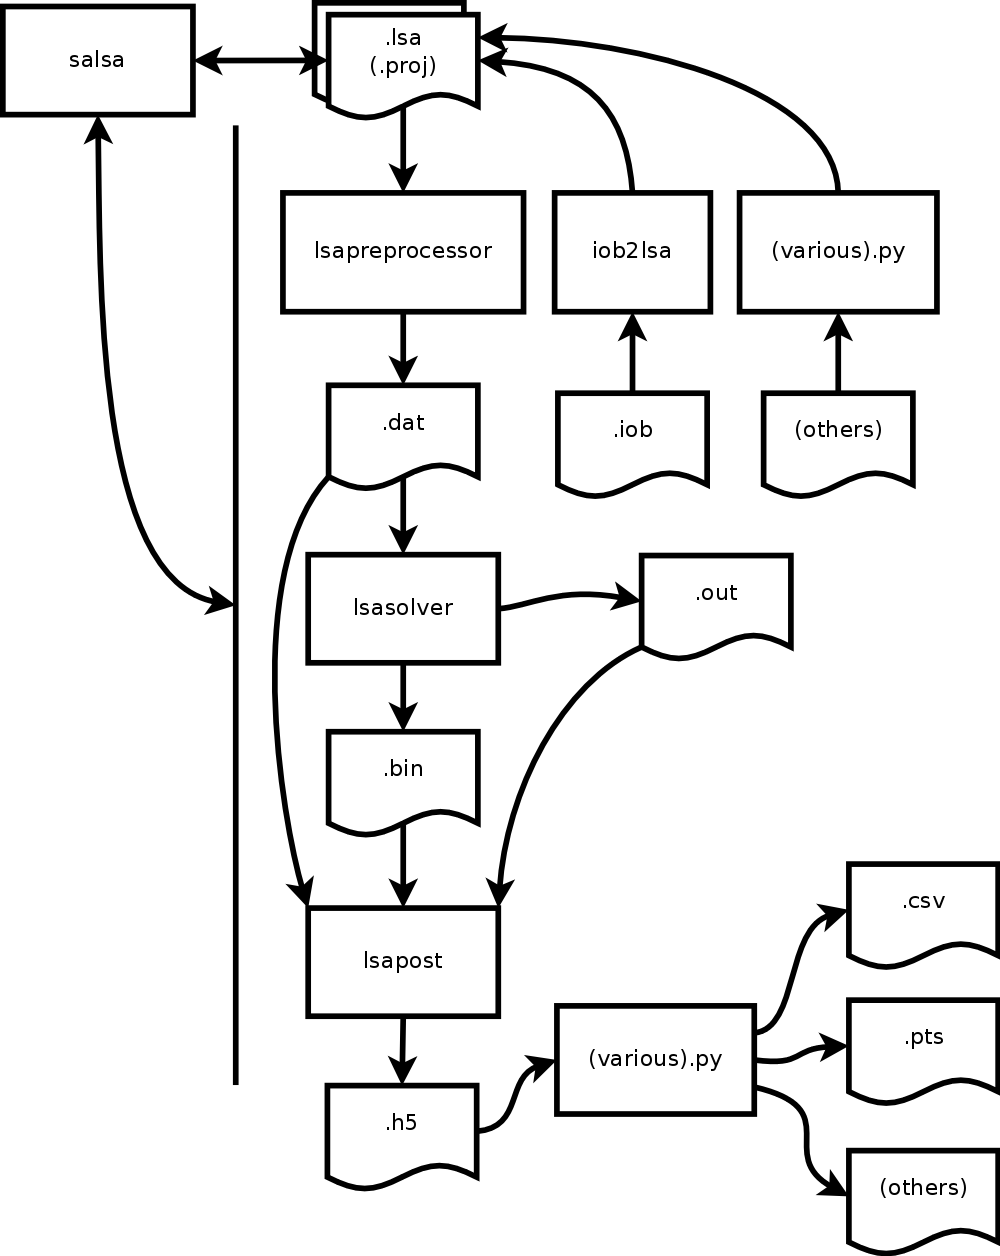
\includegraphics[width=0.8\textwidth]{Salsa_components}
\end{center}
\caption{Components of the SALSA suite.}
\label{fig:SalsaComponents}
\end{figure}

As noted earlier, \textsf{salsa} is the main GUI program that will be the focus of most users' interactions.  The GUI writes to -- and reads from -- a project file (\verb+.proj+) that fully describes the least squares problem (either alone or by including references to other \verb+.lsa+ files).  The \verb+.proj+ and \verb+.lsa+ formats are identical; \verb+.proj+ is simply chosen as a convention to signify the main project file.  See Chapter \ref{chap:LsaFormat} for details on the \verb+.lsa+/\verb+.proj+ file format.  The emphasis of Chapter \ref{chap:UsingSalsa} is how to use \textsf{salsa} to build and manipulate the least squares project (i.e., the \verb+.lsa+ files).

Once the least squares problem is set up, and the user initiates a solution, several CLI applications are executed in the background.  The first of these is \textsf{lsapreprocessor} (LSA pre-processor).  This application `flattens' the input \verb+.lsa+ files (which are relatively easy for a human to read and edit) into a single \verb+.dat+ file (which is more difficult for a human to read or edit but easy for a computer).  The main least squares solver application (\textsf{lsasolver}) is then called with the \verb+dat+ file as its input.  The solver produces two important output files: a binary file (\verb+.bin+) containing the LSA solution state, and a log file with a \verb+.out+ extension.

The \verb+.bin+ file is not human-readable, and in fact is a custom format that only the \textsf{salsa} applications can read and write.  However, the application \textsf{lsapost} ingests the contents of the \verb+.bin+ file, along with information from the \verb+.dat+ and \verb+.out+ files, and creates a more user-accessible output file adhering to the Hierarchical Data Format (HDF) standard with a \verb+.h5+ extension.  Refer to Section \ref{sec:hdfview} for instructions on obtaining a viewer for this file.

The \verb+.h5+ file has another important `audience' which is the GUI.  The \textsf{salsa} GUI reads output from the \verb+.h5+ file to provide feedback to the user and help him or her understand the results of the network adjustment.

Finally, each time a \textsf{salsa} project is processed, Python scripts read the \verb+.h5+ file and create two additional output files: a comma-separated values file (\verb+.csv+), and a simple text file listing the adjusted coordinates (extension \verb+.pts+).  The \verb+.csv+ file can be opened in a spreadsheet program to support analyses outside of SALSA and/or for copying and pasting results into a publication, and the \verb+.pts+ file facilitates quick review of the adjusted coordinates each time a solution is generated.  Additional scripts may be developed and deployed to produce other reports using the \verb+.h5+ file as the source.

To this point, we have been outlining a linear process that starts with the user working with the \textsf{salsa} interface to build and manipulate the project as captured in \verb+.lsa+ format.  Another important part of most users' workflows will be introducing measurement data that are stored in other formats.  At time of writing, many of our users have measurement data stored in the \verb+.iob+ format which is used by the program GeoLab.  Therefore SALSA includes a CLI application called \textsf{iob2lsa} that can be invoked from the \textsf{salsa} GUI to convert \verb+.iob+ files to \verb+.lsa+ format.  Several other converters are bundled with SALSA to provide direct conversion from vendors' instrument formats into \verb+.lsa+; see the appendix ``Conversion of Instrumentation Output'' for more information and a list of supported file types.

\section{Installation}

SALSA has been developed as a cross-platform application and is currently tested on Linux and Windows platforms.  However, since all of our users outside the development team use Microsoft Windows, we will limit the scope of this section to installing SALSA on Windows.

We have built SALSA for Microsoft Windows 10 64-bit. While Salsa will likely install and run on other versions of the Windows 64-bit operating system without issue, the development team currently limits testing to Windows 10.  We have not compiled a list of ``minimum system requirements.''  Instead, we offer the following guidance.  Any computer that meets the specifications for Windows 10 64-bit should support SALSA just fine.  If, however, you are solving very large problems that take more than a few seconds of processing time, your experience will likely improve if you migrate to a more powerful machine.
% TODO: see how much RAM is needed for a large problem and whether we should advise users on how much RAM they need

Installation is very simple and follows the same pattern as other applications you've likely installed before.  This section is less of a ``how to'' and is more about what gets installed, where it goes, and why it may matter.

The SALSA installer for Windows is provided as an \verb+.msi+ file.  We use the naming convention \verb+SALSA-<version>.msi+, e.g., \verb+SALSA-1.1.0.msi+.  Most users will simply wish to double-click the \verb+.msi+ file and accept default options to install the program suite.  This process will place the executables, related library files, and geoid data files into the Applications path (discussed below), will add \textsf{salsa} to the Windows Start menu, and will add a shortcut onto your desktop (which you are welcome to delete).

The default paths for installed files are as shown in figure \ref{fig:InstallLocations}.  At time of writing it is necessary to preserve the relative path structure between the \verb+bin+ and \verb+data+ directories, which will be the default state unless you manually move some of these files.  For example, the \textsf{salsa} executable (\verb+salsa.exe+) will attempt to invoke the CLI applications (the other \verb+.exe+ files in the \verb+bin+ directory) on the assumption they exist alongside \verb+salsa.exe+.  Similarly, \textsf{salsa} will expect that the geoid files exist in the adjacent \verb+data+ directory, specifically \verb+../data/geoid/<geoid_file>+.


\begin{figure}[!htbp]
\dirtree{%
.1 C:/ .
.2 Program Files/ .
.3 SALSA/ .
.4 bin/ .
.5 platforms/ .
.5 iob2lsa.exe .
.5 lsapost.exe .
.5 lsapreprocessor.exe .
.5 lsasolver.exe .
.5 salsa.exe .
.5 <lots of .dll files> .
.4 data/ .
.5 geoid/ .
.6 egm1996\_2.5m.und .
.6 egm2008\_2.5m.und .
.5 marble/ .
.5 default.cfg .
.4 doc/ .
.5 SalsaUserManual.pdf .
.4 examples/ .
.4 lib/ .
.5 lsawrappers.dll .
.4 plugins/ .
.5 marble/ .
.4 python/ .
.5 python.exe .
.5 <.dll files> .
.5 <subdirectories> .
.4 scripts/ .
.5 converters/ .
.6 wrappers/ .
.7 <python lsa wrappers> .
.6 converterlauncher.py .
.6 LeicaTotalStation.py .
.6 lsaconverter.py .
.6 PPPToLSA.py .
.6 TribmbleToLSA.py .
}

\caption{Default installed locations of key SALSA components.}
\label{fig:InstallLocations}
\end{figure}

As noted above, the installer will place the SALSA executables, library files (\verb+.dll+), geoid files, documentation, and examples under the Applications folder.  One file not yet addressed is \verb+default.cfg+.  This file contains installation-level default options germane to SALSA operation.  This file will be copied into any new LSA project created on this computer.  Of course, a user may make changes to the copied file once it is referenced in their project; the important point we wish to make here is that any configuration options that should apply to all users, for all future LSA projects created on this computer, should be done by editing \verb+default.cfg+ in this installation directory.  Doing so will require the same privileges as whoever installed SALSA.

\section{Obtaining HDFView}
\label{sec:hdfview}

Data files in SALSA are written to an HDF5 file format.  An advantage of these files is that they are easily readable with the proper HDF viewer.  We recommend using the viewer HDFView which may be obtained from The HDF Group website \cite{hdfview}.  To open an HDF5 data file which is generated by SALSA (typically, the file extension will be ``*.h5''), the user may simply double click on the file.  Alternatively the user may open HDFView and navigate to the file using File$\to$Open.

\section{Program Removal}

To remove SALSA, use the Windows Control Panel: Start $\to$ Control Panel $\to$ Programs $\to$ Uninstall a program, [right-click] SALSA $\to$ Uninstall.


% How to use it
\chapter{How to Use the salsa Interface}
\label{chap:UsingSalsa}

Recall that SALSA is a suite of applications and that the graphical user interface is called \textsf{salsa}.  This is the application that will be invoked when the user launches \textsf{salsa} from the Start menu using the cute chips-and-salsa icon, and it is the subject of this chapter.

There are three paths we can take to get LSA information into the \textsf{salsa} interface:
\begin{enumerate}
\item We can create a new LSA project.
\item We can open an existing LSA project.
\item We can import a GeoLab IOB file as a new LSA project.
\end{enumerate}


Before we explore those paths, let us introduce the \textsf{salsa} interface and point out the main parts of the interface that we'll be referencing in the following sections.  Figure \ref{fig:salsa_GUI_intro} shows the \textsf{salsa} interface with an LSA project already loaded.  The upper-left quadrant of the interface is devoted to what we call the ``Project Navigator'' which is designed to help a user view and organize all the inputs going into the least squares solution.  Since this information may be distributed across several input files, this interface employs a ``tree'' style representation of the file hierarchy, allowing the user to quickly collapse and expand each file's content.

\begin{figure}[!htbp]
\begin{center}
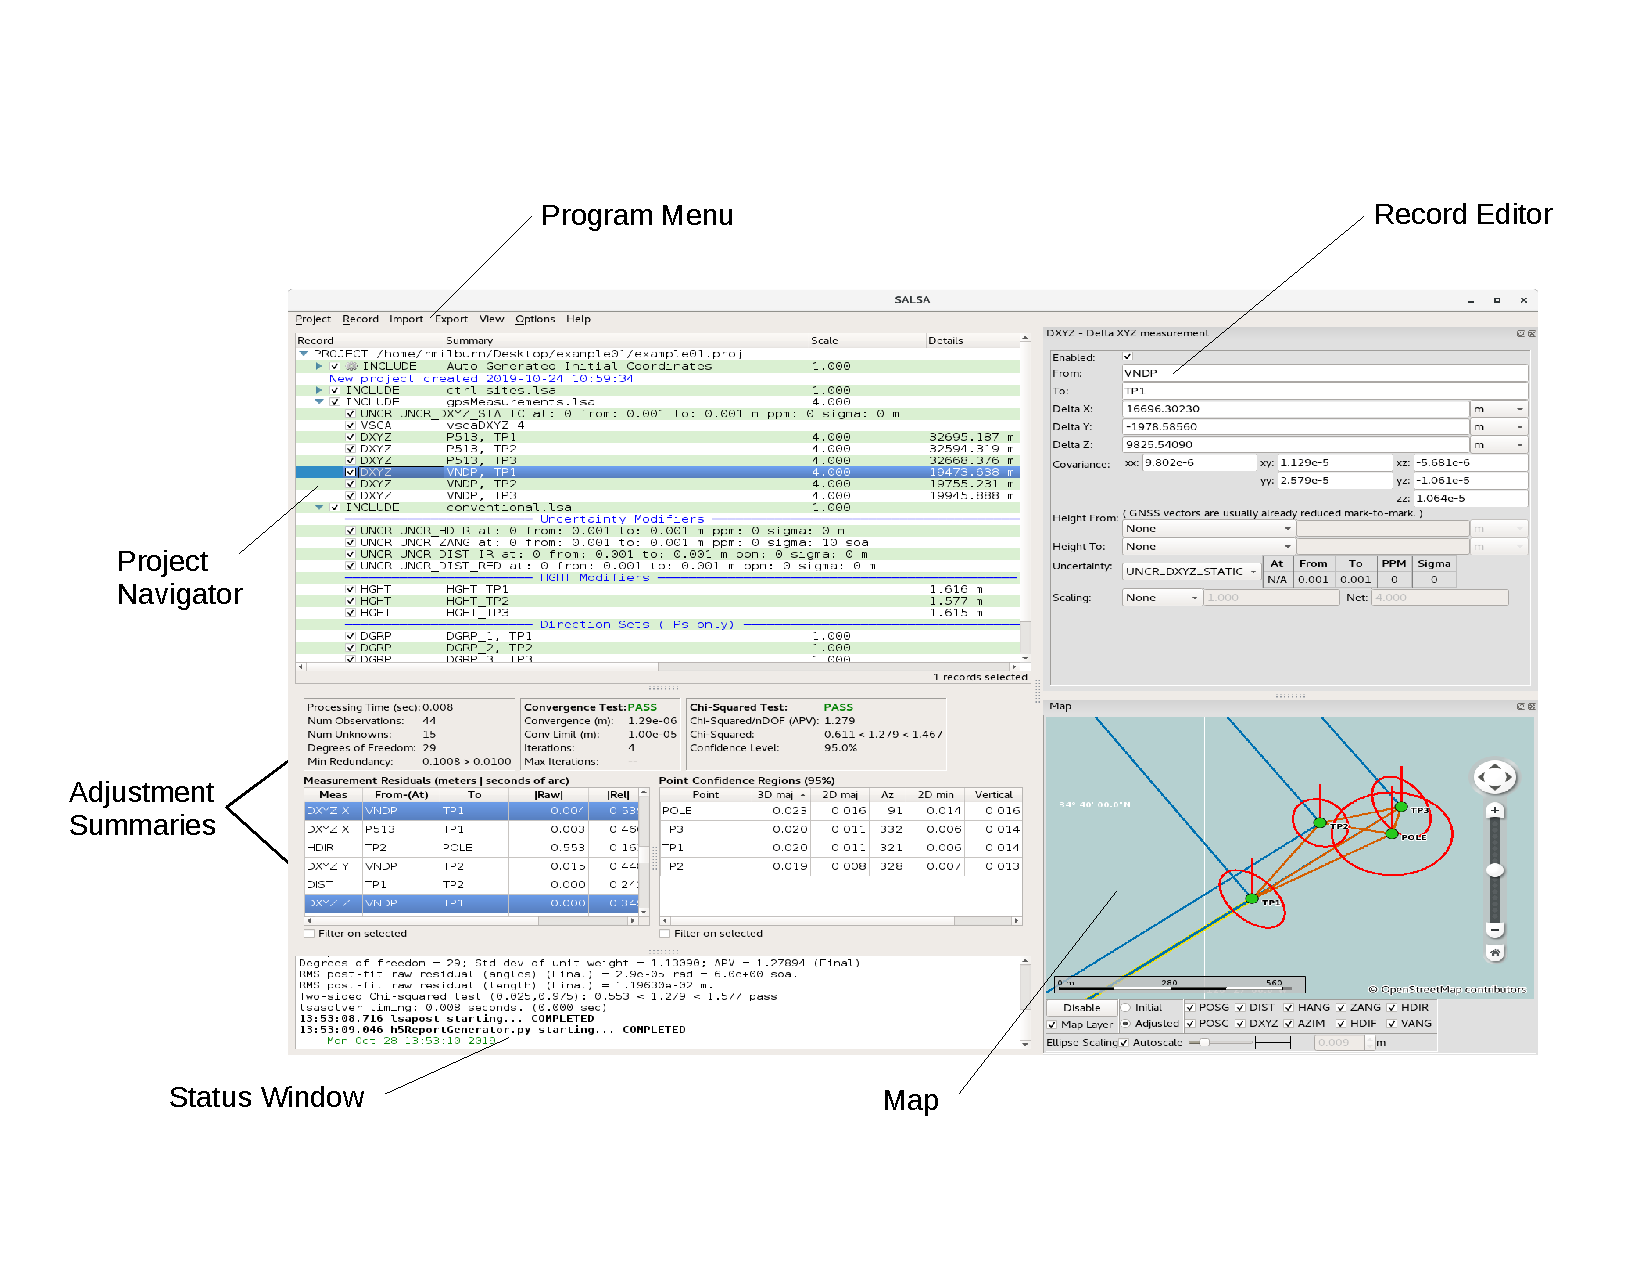
\includegraphics[width=0.99\textwidth]{salsa_GUI_intro-crop}
\end{center}
\caption{\textsf{salsa} GUI elements.}
\label{fig:salsa_GUI_intro}
\end{figure}

To the right of the Project Navigator is the Record Editor.  This interface shows the details of the currently-selected record; these details can be edited directly in this interface.

The area below the Project Navigator contains several output frames (they will be empty prior to running an adjustment).  These indicators and tables summarize the performance of the least squares adjustment and provide the user with important details when something goes wrong.  Example 1 of this user manual illustrates the utility of these indicators as a user diagnoses a problematic adjustment.

At the bottom-left of the \textsf{salsa} interface is the Status Window.  The Status Window shows output from the CLI applications that run in the background as files are opened and parsed, and as the solver runs.   For example, this window will show the iteration count and convergence level while the solver executes.  Keep an eye out for orange text, which indicates some kind of warning, and red text, which indicates an error.

The bottom-right quadrant of the \textsf{salsa} interface contains an interactive map of the survey network.  The map can render either the inputs to the LSA problem or the solution.  Example 1 of this user manual explains the map behavior in some detail and shows how the map can be helpful in understanding the LSA problem and interpreting LSA results.

At the top of the \textsf{salsa} interface we have the Program Menu that is typical of most graphical programs.  We'll go into each menu item in later sections.

Note that the user can adjust the relative size of each portion of the \textsf{salsa} interface, using the slider handles between them.  Also, the Record Editor and Map are `dockable' which means that in addition to being resizeable, they can be dragged off the \textsf{salsa} interface altogether to suit the user's screen size and preferences.  (A menu option View $\to$ Reset Windows will restore the docks to their default geometry.)

Having introduced these main parts of the \textsf{salsa} interface, let's outline the three paths for building an LSA project\ldots

\section{Creating a LSA Project}

The first path we'll explain is the process of creating a new LSA project from scratch.  When first launched, the \textsf{salsa} interface is pretty plain, as shown in Figure \ref{fig:salsa_opening_screen}.

\begin{figure}[!htbp]
\begin{center}
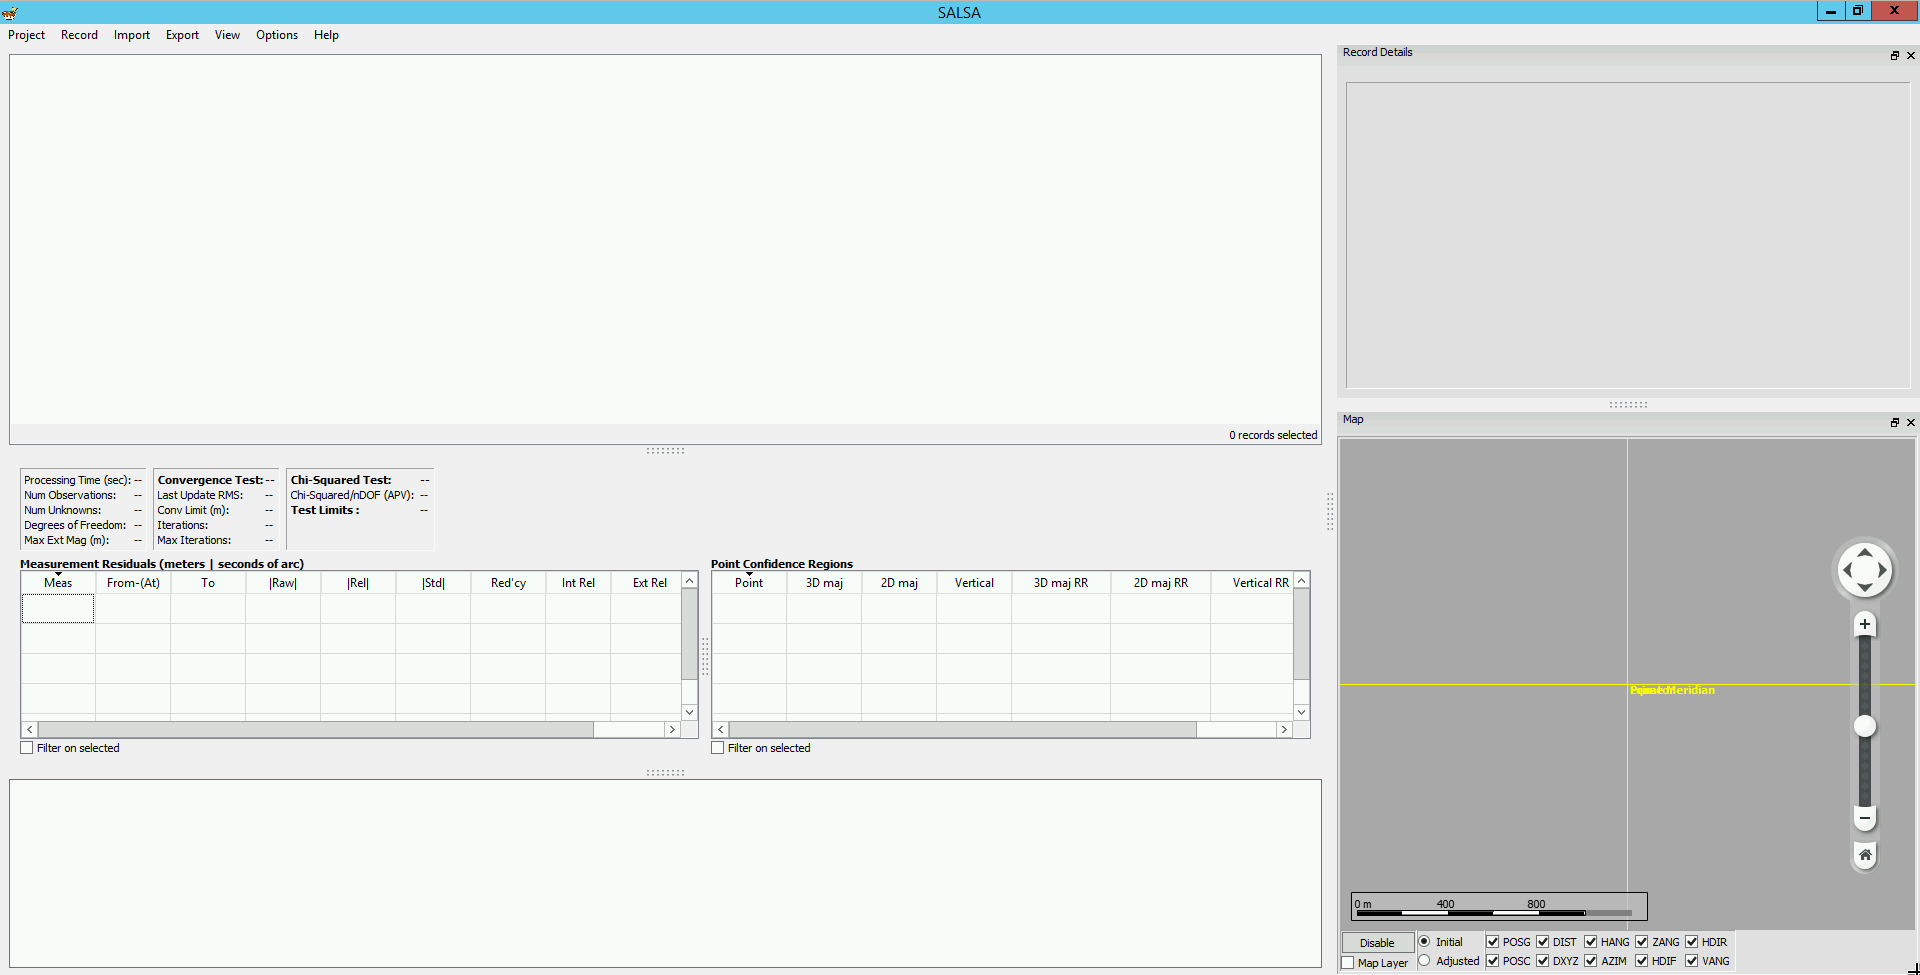
\includegraphics[width=0.9\textwidth]{salsa_opening_screen}
\end{center}
\caption{\textsf{salsa} interface on startup.}
\label{fig:salsa_opening_screen}
\end{figure}

The process of creating a new project is trivial; go to \texttt{Project} $\to$ \texttt{New\ldots}.  That will yield a file selector dialogue allowing you to navigate to a directory of your choosing (optionally creating a new one if needed) and specifying the name of the new project file.  If you don't type an extension, \textsf{salsa} will use \verb+.proj+.  When the \verb+.proj+ file is created, the file \verb+default.cfg+ will be copied from the SALSA installation directory into the same folder containing the new \verb+.proj+ file and given the same name as the \verb+.proj+ file but preserving the \verb+.cfg+ extension.  For example, if a user creates the new LSA project called \verb+newproject.proj+, the default configuration file will be copied to that same location and given the name \verb+newproject.cfg+.

When the new LSA project is created, the Project Navigator will show the name of this new top-level project file and its contents, which at first will be limited to a single comment indicating the date and time the project was created.  From this point, the user can start adding survey records or other files containing survey records.  Reference Example 1 of this user manual for a complete illustration of this path.

% Do we really want to walk through examples at this point?  I don't think so - that will be slow and tedius.
% We just want to explain the paths at this point.

\section{Opening an Existing LSA Project}
\label{section:OpeningProject}

An existing project can be opened via the menu option \texttt{Project} $\to$ \texttt{Open LSA\ldots}.  This will present a file browser prompting the user to identify an existing \verb+.proj+ or \verb+.lsa+ file to load.  Any existing content in the \textsf{salsa} interface will be cleared, and this file will be treated as the top-level project file.  If a SALSA configuration file by the same name (but with \verb+.cfg+ extension) does not already exist at this location, it will be copied from the SALSA installation directory.

When a \verb+.proj+ or \verb+.lsa+ file is opened, all records in the file are parsed and displayed in the Project Navigator.  This includes any included files and their records (and their included files, etc.).

As those lsa-formatted files are opened and parsed, any problems will be reported in the Status Window at the bottom of the \textsf{salsa} interface.

Note that \emph{opening} an LSA project file (\verb+.proj+ or \verb+.lsa+) is not the same as \emph{including} an LSA file within an existing project.  Example 1 of this user manual involves the inclusion of \verb+.lsa+ files into an existing project. 

\section{Importing a GeoLab IOB Project}

\textsf{salsa} also provides support for loading an LSA project from GeoLab \verb+*.iob+ format.  This action is initiated via the menu option \texttt{Project} $\to$ \texttt{Open Geolab Project\ldots} which will prompt the user to select the top-level GeoLab project (likely named \verb+*.iob+) and will then perform the following actions:
\begin{enumerate}
\item \textsf{salsa} will set the new LSA project directory to the location of the specified \verb+*.iob+ project file.
\item \textsf{salsa} will convert the top-level \verb+*.iob+ file into LSA format, giving it the extension \verb+.proj+.
\item \verb+default.cfg+ is copied into the project directory just as is done when a new LSA project is created.
\item Any files that were included (\verb+#INCLUDE+) in the imported \verb+*.iob+ file will also be converted into \verb+.lsa+ format, yielding a project structure in LSA format that should closely match the original IOB organization.
\end{enumerate}

\section{Dropping Data in the Project Navigator}
As an alternative to opening files as described in section \ref{section:OpeningProject}, users can also drag files from outside of \textsf{salsa} and drop them into the Project Navigator to include them in the current project.  Conveniently, if a file is not already a \textsf{.lsa} or \textsf{.proj} file, \textsf{salsa} will attempt to determine the file's type and use the appropriate built-in file converter to include it into the current project.  Avoid dropping files which would already be included as a child of another file being dropped.

\textsf{salsa} can also open a dropped file as the top-level project if there is not one already open. In the case that more than one file is dropped on an empty Project Navigator, the user will be prompted to create a new \textsf{.proj}.  This will become the top-level project for the files being dropped.

Plain text can also be dragged and dropped onto the Project Navigator if there is already a project open.  This is especially useful when the user wants to take records from one project open in a text editor and duplicate them in a project open in \textsf{salsa}.  The records are added on a line-by-line basis.  If the line is not a file include (\textsf{-{}-include filename}) or does not begin with an appropriate record tag (e.g. \textsf{POSG}, \textsf{AZIM}, etc. See chapter \ref{chap:LsaFormat}), it will be added as a comment. When dropping an include as text (\textsf{-{}-include filename}), the file specified by \textsf{filename} must be in the currently opened top-level project's directory, or \textsf{filename} must contain the relative filepath (e.g. \textsf{-{}-include subDir/filename}).

\section{Editing Records}
When a record is selected in the Project Navigator, the Record Editor is populated with the information contained in that record, and many of the controls are user-editable.  The appearance of the Record Editor will vary based on the type of record selected, of course, because different record types contain different information.  The developers hope that these interfaces are sufficiently intuitive that we need not bloat this user manual with field-by-field explanations and screen shots for each record type.  That said, some records exhibit behavior that may not be obvious to all users, so we feel compelled to explain the design choices and program behavior in these cases.

\section{Find/Filter Records}
The user may find that they want to select only AZIM records in a large project. It would be tedious to scroll through all of the records and through all of the includes. This is where the Find/Filter widget comes in handy. To open this widget, click \verb+Record+$\rightarrow$\verb+Find/Filter...+ (or Ctrl+F) with a project already open.

Notice that the Find/Filter widget has a Find row and a Filter row. Each of these sport their own text field, in which the user can specify their search terms. There can be multiple search terms simultaneously, each separated by a space. Terms surrounded by quotes are considered as one term, regardless of spaces within. The interpretation of the search terms can be manipulated by the 'exact match` checkboxes. When checked, the results will only include records which match exactly. For example, if the user searches for "TGT01", records which contain "TGT01" would be returned but not those containing "TGT011". Find and Filter both have ANY/ALL dropdowns, which are useful for specifying how multiple search terms should be handled. If the user selects ANY, then a given record is included if at least one of the search terms match. Conversely, the ALL option ensures that only records which match all search terms are included.

The Filter option has another dropdown with a default value of 'All Records'. The options in the dropdown are simply a quick way to filter based on a record type or other common feature of a record (e.g. enabled or disabled).  The Find row of the widget provides an 'All' button. This button will select all records in the Project Navigator which match the search. The arrow buttons will singly select the next or previous record which matches the search. Finally, the warnings button will change the user's selection to the next record which has a warning.

Note that the Filter and Find functionality can be used in conjunction: the Find feature will only select records which are available after the Filter has been applied.

\section{Record Modifiers}

There is a class of records that we call ``modifiers'' because they affect other records.  Thus, there are some design choices embodied in \textsf{salsa} that users should understand.  These ``modifier'' record types include the following:
\begin{itemize}
\item HGHT (Height of Instrument/Target)
\item VSCA (Variance Scaling)
\item UNCR (Uncertainty Model)
\item DGRP (Direction Group)
\end{itemize}


In general, when the value of a modifier is changed, that change will immediately apply to any records referencing that modifier.  For example, suppose we create a height of instrument record (HGHT) for station TP02 for a set of morning total station observations, and we give it the label ``TP02-morn'' and the value of 1.550 m.  Measurement records collected with that configuration will specify TP02-morn for the corresponding height of instrument, and the value 1.550 m will be displayed in the record editor.  Reference Figure \ref{fig:modifiers_propagating}.  Suppose however that we realize 1.550 was the height measurement made for an afternoon observation set, and the morning height was actually 1.402.  We can correct the TP02-morn HGHT record to reflect that value; at this point the corrected value of 1.402 m will be effective for all measurements referencing the TP02-morn height record.

\begin{figure}[!htbp]
\begin{center}
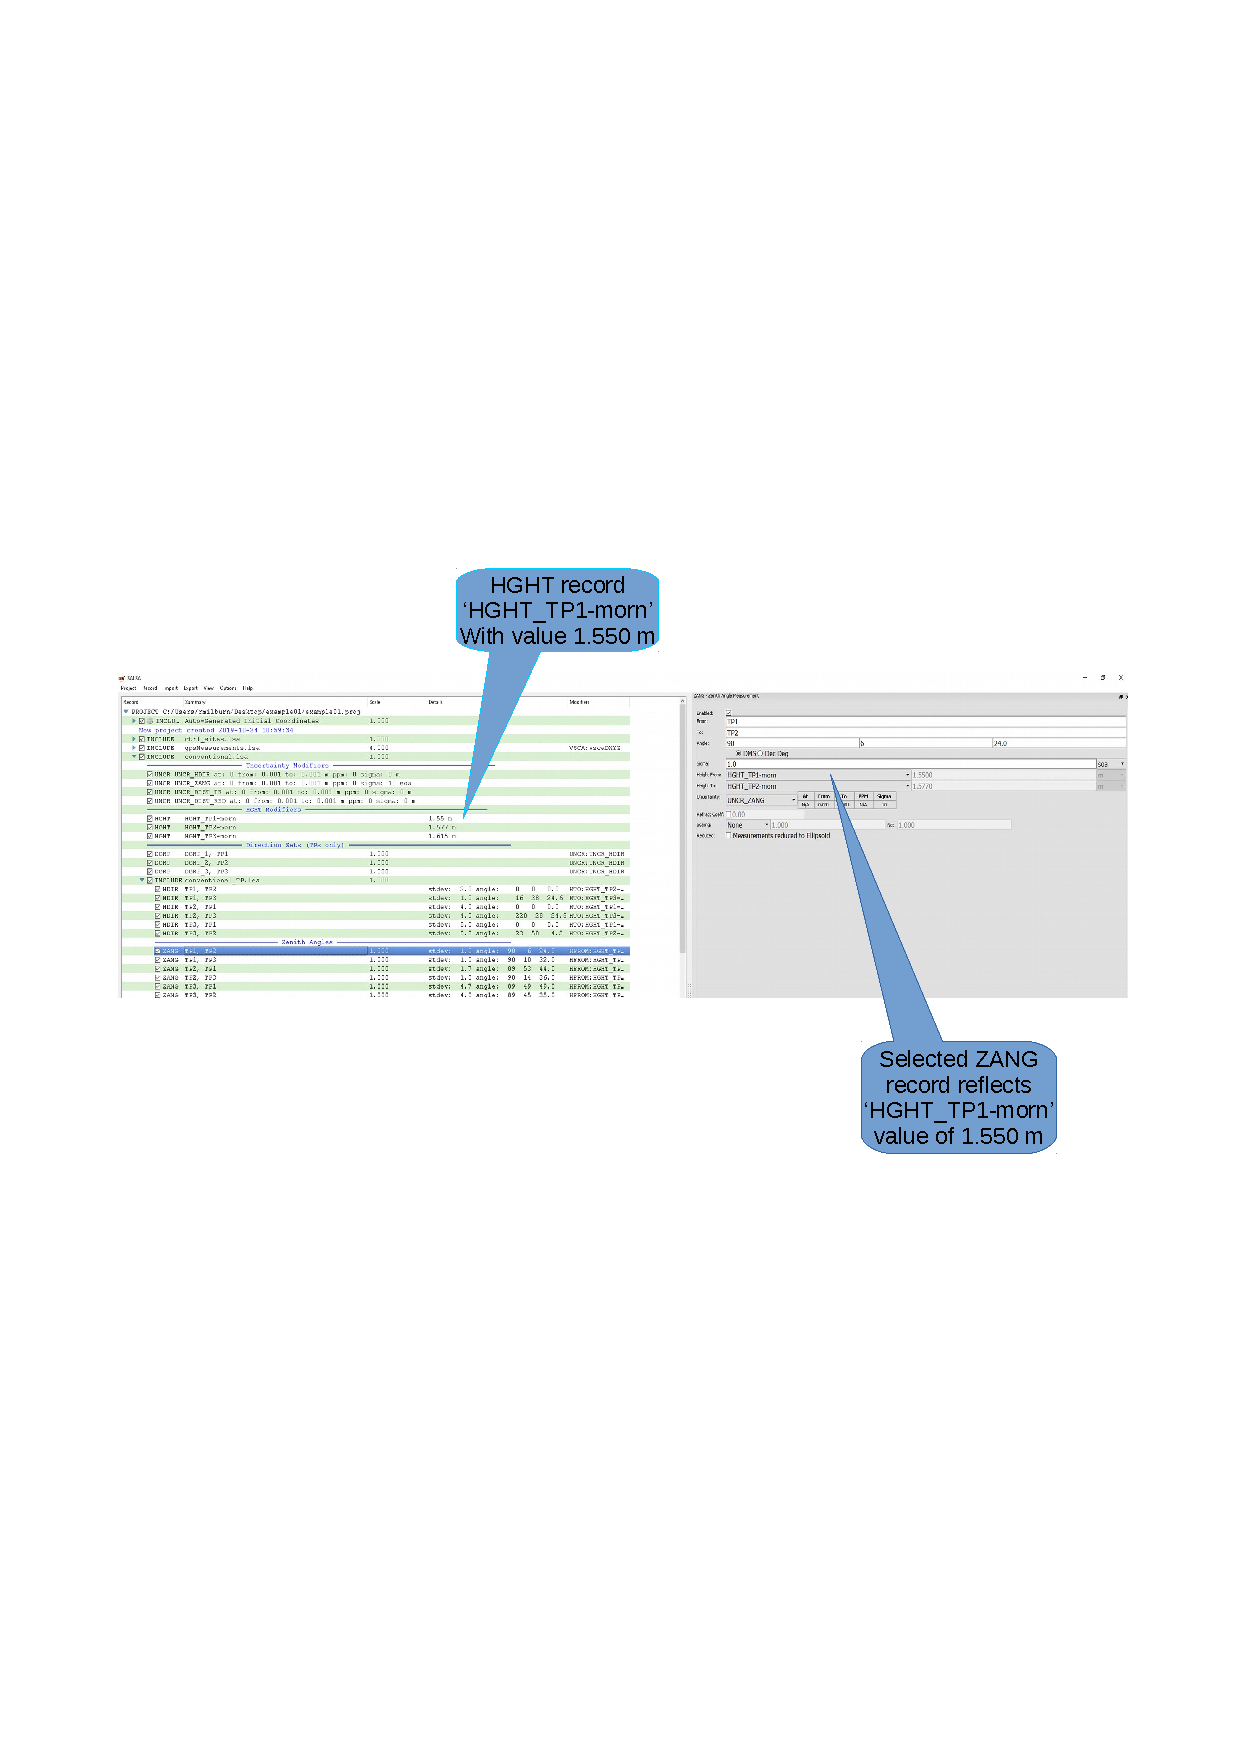
\includegraphics[width=0.88\textwidth]{modifiers_propagating-crop}
\end{center}
\caption{The numerical value for a modifier, such as height of instrument/target (HGHT), will immediately reflect any changes made to that modifier record.}
\label{fig:modifiers_propagating}
\end{figure}

Similarly, changing a modifier label will immediately apply to all records referencing that label.  Working with the previous example, if we change the HGHT record label from ``TP02-morn'' to ``TP02-morning'' all records referencing ``TP02-morn'' will immediately be updated to reference ``TP02-morning.''

Table \ref{tab:ModifierBeahvior} lists common edits one might make to a modifier record and the corresponding result of that edit.

%\begin{table}[htb]
\begin{table}[!htbp]
\caption{Effects of Editing Modifier Records}
\label{tab:ModifierBeahvior}
\begin{center}
\begin{tabular}{p{2.25 in}p{2.75 in}}
\hline
\textbf{Action} & \textbf{Result} \\
\hline
Alter the value of a modifier (HGHT, VSCA, UNCR) & The new value becomes effective in all records referencing this modifier. \\
Alter the name/label of a modifier & All references in the project to the old label will be updated to reflect the new label. \\
Delete a modifier (HGHT, VSCA, UNCR) & All references in the project to the deleted modifier will be removed, e.g., a reference to a HGHT record will become None and assume a value of zero. \\
Delete a Direction Group (DGRP) & The Direction Group and all children (horizontal directions referencing the group) will be deleted. \\
\hline
\end{tabular}
\end{center}
\end{table}


\section{Project Configuration}
When a new LSA project is created, a default configuration file is copied from the \textsf{salsa} installation directory into the project directory.  This file is used by the solver to determine, among other things, the formatting of the output.  It is also used by the post-processor.  If the user wishes to change the way that output is formatted, for example, this default configuration may be altered by selecting the \texttt{Project} $\to$ \texttt{Configure\ldots} menu option.  This will display the Project Configuration panel.

\begin{figure}[!htbp]
\begin{center}
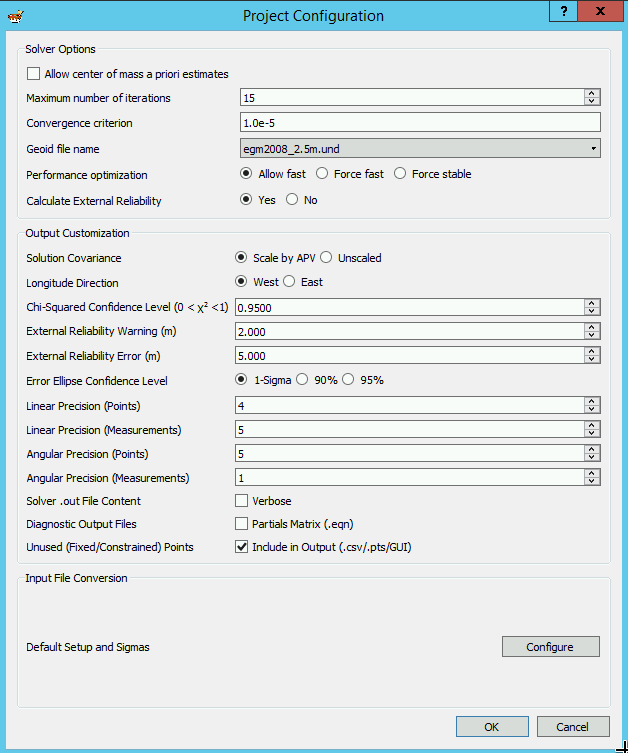
\includegraphics[width=0.9\textwidth]{ConfigPanel}
\end{center}
\caption{Default configuration for a priori position generation, solver options, and output customization.}
\label{fig:config_panel}
\end{figure}

The user may also change the default configuration that is used when converting instrumentation output into the LSA format.  To do this, press the Configure button from the Input File Conversion section of the Project Configuration panel.  This will bring up the LSA Converter Measurement Uncertainty Configuration panel.

\subsection{Converter Configuration}
\label{subsect:convert_config}
Just as there is a configuration file that is used by the solver and post-processor to determine the format of the output of those programs, among other things, there is also a configuration file, \verb+converter.cfg+, that is used to determine the output of the instrument output-to-LSA converters.  This file determines the centering error values for UNCR records associated with particular measurement types for particular instrument types, as well as the sigma values to assign to different measurement types.

\begin{figure}[!htbp]
\begin{center}
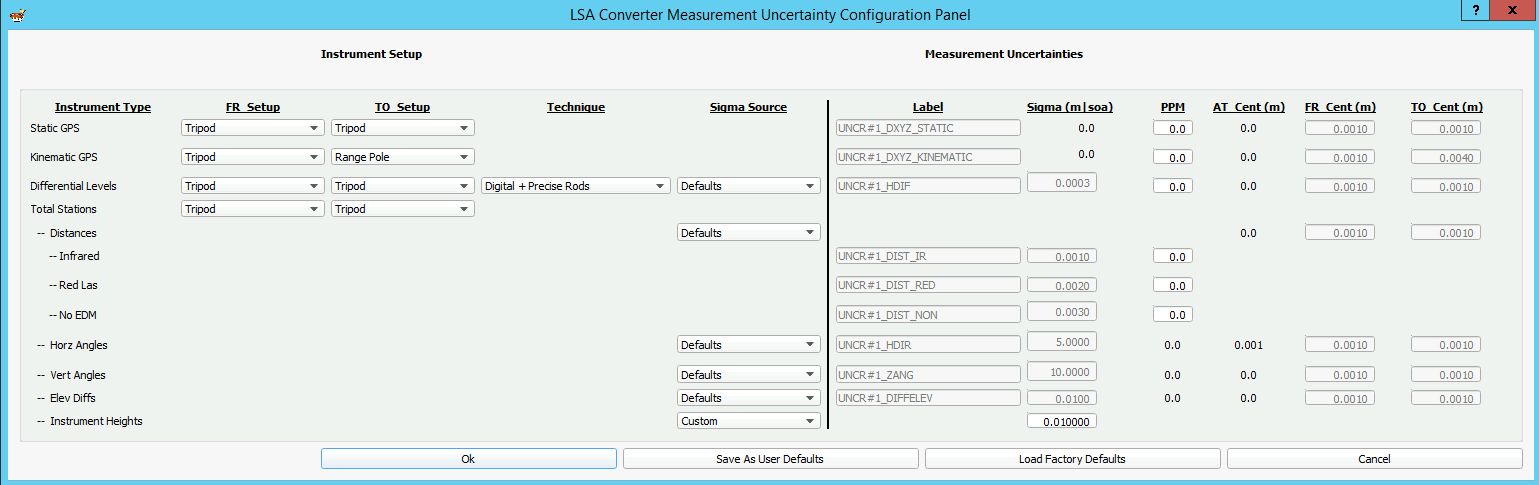
\includegraphics[width=0.9\textwidth]{ConverterConfigPanel}
\end{center}
\caption{Default configuration of UNCR records and measurement sigmas when converting instrument output to the .lsa format.}
\label{fig:converter_config_panel}
\end{figure}

The default values for these UNCR records may be changed by changing the setup types for the FROM and TO stations of a particular measurement in the LSA Converter Measurement Uncertainty Configuration panel.  The hardware-dependent default sigmas and centering errors are defined in the following table.  The user is also able to enter their own centering errors by selecting the Custom setup option from the respective combobox.

\begin{table}[!htbp]
	\caption{Setup-dependent centering errors}
	\label{tab:CenteringErrors}
	\begin{center}
		\begin{tabulary}{4.5 in}{LL}
			\hline
			\textbf{Setup Type} & \textbf{Centering Error (m)} \\
			\hline
			Forced Centering Plate & 0.0 \\
			Range Pole & 0.004 \\
			Tripod & 0.001 \\
			Vertical Collimator & 0.0005 \\
			\hline
		\end{tabulary}
	\end{center}
\end{table}


Similarly, the user may change the default sigmas assigned to particular measurement types by changing the sigma source from Defaults to Instrument, which uses the instrument-reported sigma values, or Custom, which allows the user to enter their own sigma values to assign.  The sigma defaults are defined in the following table.

\begin{table}[!htbp]
	\caption{Default Sigmas by Measurement Type}
	\label{tab:DefaultSigmas}
	\begin{center}
		\begin{tabulary}{4.5 in}{LLL}
			\hline
			\textbf{Measurement Type} & \textbf{Technique} & \textbf{Sigma (m or soa)} \\
			\hline
			Differential Levels & Digital + Precise Rods & 0.0003 \\
			Differential Levels & Digital + Standard Rods & 0.0006 \\
			Differential Levels & Spirit + Standard Rods & 0.001 \\
			Distances & Total Station Infrared & 0.001 \\
			Distances & Total Station Red & 0.002 \\
			Distances & Total Station No EDM & 0.003 \\
			Horizontal Angles & Total Station & 5.0 \\
			Vertical Angles & Total Station & 10.0 \\
			Elevation Differences & Total Station & 0.01 \\
			Instrument Height & Measuring Rod & 0.001 \\
			Instrument Height & Measuring Tape & 0.001 \\
			\hline
		\end{tabulary}
	\end{center}
\end{table}


The user may use this panel to set up their own defaults that will persist from project to project by pressing the Save As User Defaults button.  To save the configuration just for the open project, without modifying the user defaults, press the Save As Project Config button.  To restore the panel to the factory defaults, press the Load Factory Defaults button.  The Save As Project Config button should be pressed to generate the converter.cfg file prior to importing the instrument output files.





% TODO
% condition number
% divergence
% minimal constraints
% references
% examples
% bancroft citation


\chapter{Understanding the Solver}
\label{chap:UnderstandingSolver}

This chapter describes the command line program \textsf{lsasolver} (``the solver'') that serves as the estimation engine of SALSA, what it does, and (briefly) how to understand the output. The solver was developed using \cite{ghilani} as the primary reference; this is an excellent reference and the user interested in more detail on the topics discussed here is referred there and to \cite{leick}.

\section{What the solver does}
The solver performs the fundamental task of using the input measurement and initial position data to find an optimal solution (adjustment) for the positions. In addition it finds an initial position for unknown sites, performs quality assurance and statistical tests on the data and the adjustment, and does geoid computations.

The solver input data is contained in a flat text file (the ``DAT file,'' usually with extension \verb+.dat+) with its own format as documented in Chapter \ref{chap:datref}, ``The *.dat File Format Specification.'' The format is quite simple and consists of one complete position or measurement per line.

\textsf{salsa} automatically uses the \textsf{lsapreprocessor} program to generate this file, and then passes it as input to the solver, behind the scenes, whenever it is directed to run a computation. However the file may be edited or even created in a text editor and then given as input to the solver being run on the command line.

The solver begins by parsing the input DAT file and collecting positions and measurements. Any error in the DAT format yields an Error message in the solver output, indicating that a record (line) could not be parsed (but the solver does not abort).

Each site must have a unique label, given either in the POS record for that site (containing an initial value for the site's position), or as it is used in one or more measurement records. Each site also has a type, which is one of the following.
\begin{description}
\item[Fixed] Generally some, but not all, sites are fixed (``control points''); these sites' coordinates are held fixed in the network adjustment.
\item[Estimated] These sites' coordinates float and will be estimated in the adjustment.
\item[Adjusted] These sites can serve as control points in the network, but their position will be adjusted in the estimation, using the given \emph{a priori} position as data; this option is often used for GNSS-determined point positions. POS records that are to be adjusted must have a non-zero covariance.
\item[Unknown] Other sites lacking POS records but encountered in the network (i.e., because they are referenced by one or more measurements) will be initially ``unknown.''  Once initial coordinate estimates are generated (using methods described below), these points will be treated as Estimated.
\end{description}


The first task for the solver, after reading the input, is to compute initial estimates, or \emph{a priori} positions for all the unknown sites. (These positions are required because the least squares problem is non-linear and so must be iterated, which requires a starting value for all the positions; see Section 4.3 below.) The algorithm for doing this depends on what data are available that involve the unknown site. The solver tries to use each of ten different algorithms and all the measurements in the input to find each unknown site's \emph{a priori} positions. All the successful results for that site are then averaged to give the final \emph{a priori} position. The type indicator for the site is then changed from ``unknown'' to ``to be estimated.'' If an \emph{a priori} position for any site(s) cannot be found, then the solver must terminate with an error, since the adjustment cannot be performed. The ten \emph{a priori} algorithms are documented below in Section \ref{sec:apriorialgorithmsec}.

The solver computes a weighted least squares solution to the adjustment problem using all of the measurement data, with measurement covariance, and perhaps with constraints. This is a full 3-dimensional computation in the WGS84 geodetic frame using Earth-Centered Earth-Fixed Cartesian coordinates (ECEF XYZ). Control sites with type ``to be adjusted'' are used to generate pseudo-data that allows the given position to be included in the estimation. Constraints may be applied prior to the estimation computation; that is, sites may be constrained to remain fixed in any combination of (one or two) components North, East and Vertical (see the POS record ``CONS'' documentation in the DAT file specification in Chapter \ref{chap:datref}).

The least squares estimation yields not only an optimal estimate of the adjusted positions, but also (assuming degrees of freedom greater than zero, see Section \ref{sec:leastsquaressec}) an estimate of the uncertainty on these results. Statistical tests can be performed on the results to give an indication of the quality of the adjustment, which is determined by the quality and quantity of the data. These statistical tests can be used to determine if the relative weighting of data should be adjusted or if the data or control points contain blunders or improper initial uncertainty estimates.

The solver presents all of this information in a human-readable flat text output file, including tables of residuals, statistics, and adjustments with their uncertainties and covariances.

\section{Least squares}
\label{sec:leastsquaressec}
The estimation algorithm used by the solver is ``iterative linearized weighted least squares;'' this section attempts to explain all of that. Basic weighted least squares is described first, followed by the statistical results and tests that can be derived from it. Next the iterative solution of the full non-linear adjustment problem is described.

\subsection{Basic least squares} \label{sect:BasicLeastSquares}
The least squares method solves the linear algebra problem of several equations relating unknowns (the state vector) to measurements (the data vector). If a covariance matrix (measurement uncertainties) for the data is available, the solution can be weighted, which means varying degrees of importance are given to different data elements, potentially yielding a better solution.

%Least squares requires that there be more data than there are unknowns in order for a solution and covariance to exist.
When employing a least squares method, there must be the same amount or more data than there are unknowns for a solution to exist, and more data than there are unknowns for a covariance to exist. The number of degrees of freedom is
\begin{equation}
N(dof) = N(data) - N(unknowns)
\end{equation}
If the degrees of freedom is negative, the problem is under determined and there is no solution, if it is zero the problem is evenly determined and there is a solution but it is exact and residuals are all zero (statistics cannot be computed); all of the measurement noise is passed through to the solution. Least squares estimation methods are typically employed for over determined problems (i.e. the number of degrees of freedom is positive). More degrees of freedom generally yeilds a better solution because there is more input information (measurements) and noise in the solution is reduced (think of averaging). 
%The normal operation of least squares is for over determined problems where the degrees of freedom is positive.

In the case of the solver, the set of equations to be solved is simply the set that relates all of the measurements (angles, distances, 3-D deltas, heights, etc) to the coordinates of the sites involved in the measurement \cite{ghilani} \cite{leick}. These equations are written as a matrix equation relating the state X (a vector of all the coordinates of all the non-fixed site positions) to the data d (a vector of all the measurements). The matrix is called a ``partials matrix'' P (for a reason to be given below). Thus the matrix equation to be solved is
\begin{equation}
P \cdot X = d
\end{equation}
The solution to this problem is simply
\begin{equation}
\begin{split}
Cov &= (P^T \cdot P)^{-1} \\
X &= Cov \cdot P^T \cdot d
\end{split}
\end{equation}
where Cov is the covariance of the solution X. A vector of data residuals is simply
\begin{equation}
R = d - \hat{d} = d - P \cdot \hat{X}
\end{equation}
These residuals are the difference of the measured data and the value that would be computed from the solution for the final adjusted positions. Generally if a residual is larger than the uncertainty in the data that was input to the problem, then either the measurement is bad or the uncertainty is too small.

In weighted least squares, the equations are multiplied by a weighting matrix W (usually W is equal to the inverse of the measurement covariance matrix MCov) before the solution is formed, so then the result is
\begin{equation}
\begin{split}
W &= (MCov)^{-1} \\
Cov &= (P^T \cdot W \cdot P)^{-1} \\
X &= Cov \cdot P^T  \cdot W \cdot d
\end{split}
\end{equation}
The weighting has the effect of changing the relative strength of the data in the estimation; that is, data with a larger weight (smaller measurement variance) has a stronger influence in the determination of a solution. Note that the word ``relative'' is crucial in the previous sentence; in fact if the entire measurement covariance matrix $MCov$ is scaled, this same scale multiplies the resulting solution covariance $Cov$ but has no effect at all on the solution vector $X$.

\subsection{Statistics: APV and Chi-squared}
[Note this section and the next assume degrees of freedom greater than zero.]

The fact that least squares is insensitive to the overall scale of the covariances (measurement and solution) would seem to imply that this overall scale must remain unknown. This is not the case; one of the marvelous things about least squares is that it yields not only a solution with (relative) covariance, but also an optimal estimate of the overall scale of the solution covariance. This scale is called the ``\emph{a posteriori} variance of unit weight'' or APV.

The APV is the ratio of the overall scale of the solution and measurement covariances; it is computed using the RMS relative residual and the degrees of freedom. The full, properly scaled solution covariance is thus $APV \cdot Cov$. Ideally the APV should turn out to be 1. If the APV is ~1.0, the problem is weighted correctly and so the solution is optimal. If it is too large, then some or all of the measurement uncertainties are too large, and a somewhat sub-optimal solution has been produced. If it is too small, then the measurement uncertainties are too small (this is discussed further below).

The APV and degrees of freedom are used in a statistical test of the correctness of the adjustment, the $\chi^2$ or Chi-squared test. The test statistic is equal to the APV multiplied by the degrees of freedom, and the test is to compare it to the value of the $\chi^2$ inverse cumulative distribution \cite{NIST} function (or just $\chi^2$ function). This is a well known special function in mathematics \cite{ghilani} \cite{abramowitz} \cite{NIST} that depends on both the degrees of freedom and a confidence level $\alpha$.

The confidence level is a probability, so $0 \leq \alpha \leq 1$; usually $\alpha$ is expressed as a percentage. The statement of the Chi-squared test is ``if the test statistic is less that the Chi-squared function with n degrees of freedom and confidence $\alpha$, then the adjustment is optimal with confidence $\alpha$'' \cite{ghilani} \cite{leick}. (Note that the solver output shows the Chi-squared test with the the degrees of freedom divided out; it does this just to keep the numbers relatively small.)

The test is basically to see if the solution lies within the tails of the Chi-squared function. This can be done at the upper tail ($\alpha$ is large, say 95\verb+%+) or the lower tail ($\alpha$ small, say 5\verb+%+). A ``two-sided test'' can also be performed, in which the confidence is split between the two tails and both tests are shown.

\subsection{The problem is non-linear}
\label{sec:nonlinsolver}
The diligent reader may have noticed that in fact the measurement equations cannot be written as above, $P \cdot X = d$, because they are non-linear in the site coordinates. This is true; the adjustment problem is actually a non-linear one, $f(X) = d$, where the function $f(X)$ is non-linear, and so basic least squares does not apply. However non-linear problems can be still be solved with least squares; the procedure is to first linearize the problem, then iterate the basic least squares algorithm until it converges to a final solution.

The non-linear equations are linearized by starting with an initial, or \emph{a priori}, solution (maybe just a guess). An initial state vector is \emph{required} for non-linear problems; it should be as accurate as possible (but many inaccuracies can be made up for by more iterations).

Call this initial state $X_0$, and write the non-linear function as a Taylor expansion about this initial value, as follows.
\begin{equation}
f(X) = f(X_0) + \frac{\partial f}{\partial X}|_{X_0} \cdot \triangle X + O(\triangle X^2) = d
\end{equation}
Assume that the change in state $\triangle X$ is small, and so keep only the linear term in the expansion; then the equation $f(X) = d$ becomes
\begin{equation}
\frac{\partial f}{\partial X}|_{X_0} \cdot \triangle X = d - f(X_0)
\end{equation}
But this is now of the form of the basic least squares linear equation, with partials matrix $P = \frac{\partial f}{\partial X}|_{X_0}$ and new data vector $d - f(X_0)$. (This is why it is called the partials matrix, because it is a matrix of partial derivatives.)

We can now solve for the change in state using ordinary weighted least squares. But because the change in state $\triangle X$ has been assumed to be small, we must iterate this process until it converges, meaning until the change in state is very small. Thus the final solution is obtained via an iterative, linearized, weighted least squares algorithm, as follows.
\begin{enumerate}
\item Obtain an \emph{a priori} solution $X_0$ for the unknown sites, along with data and measurement covariance, and set $i = 0$.
\item Compute the partials matrix at $X = X_i$ and the data vector $d - f(X_i)$.
\item Use weighted least squares to solve the linearized equation for the change in state, $\triangle X$.
\item Test the size of $\triangle X$; if it is very small, quit with success. $X_i$ is the solution, with covariance $Cov = (P^T \cdot W \cdot P)^{-1}$.
\item If the number of iterations becomes large, or if $\triangle X$ starts to grow, quit with failure.
\item Replace $X_i$ with $X_{i+1} = X_i + \triangle X$, increment $i$ and go to step 2.
\end{enumerate}

There are many ways to implement and solve the least squares equation, some more stable and efficient that others. Simple matrix multiplication and inversion is not the best way. The solver provides the flexibility to use methods optimized for speed, or the most stable algorithm known, which involves Cholesky decomposition or matrix square roots and the Householder algorithm \cite{biermann}.

\subsection{Constraints}
The position of any site can be fixed via the keyword FIX of the POS record in the DAT file; this means the site is not adjusted. Alternatively, just one or two of the components (North, East, Vertical) may be fixed, and the other(s) left free to be adjusted, by using the keyword EST (to be estimated) and adding constraints in the POS record using the keyword CONS (cf.Chapter \ref{chap:datref}).

Constraints actually strengthen the estimation, by adding information in the form of constraint equations. This is apparent in the degrees of freedom, which becomes, in the presence of constraints on some number of components,
\begin{equation}
N(dof) = N(data) - N(unknowns) + N(constraints)
\end{equation}

A constrained adjustment will yield not only a zero adjustment, of course, but also a zero uncertainty, for the constrained component(s). Thus in the Final tables of adjusted positions (see below), the sigma for the constrained component will read zero or extremely small, and the covariance matrix for the constrained position will be singular (the XYZ covariance will probably not have zeroes in it, but will in fact be singular).

These constraints are implemented in a strictly rigorous way using matrix decomposition and projection. This has the effect of limiting the vector space of the least squares solution to the subspace in which the constraints are exactly satisfied. This is unlike other techniques for applying constraints that use ``overweighting'' or pseudo-data with zero covariance to force the least squares solution to hold components fixed \cite{ghilani}; these methods are inexact and run the risk of destabilizing the problem and even making it singular.

%Minimal constraints are used to test for blunders in the data and the control points. They consist of a set of 3 constraints involving only two sites; one site is fixed and the azimuth and vertical angle between the first and second sites is also constrained. All other sites are allowed to move, i.e. set as ``to be estimated.'' This is a minimal set of constraints because it only prevents the network of positions from rotating an translating; all other possible adjustments, including overall scaling of the network, are allowed. A minimally constrained solution allows the maximum amount of adjustment to occur, so sites that might be control points are allowed to adjust. Thus blunders or large errors in the data and even the control points can be pointed out. The solver implements minimal constraints using a command line option (minCon).

\section{A priori computations}
\label{sec:apriorisection}
The solver makes use of ten different algorithms that can possibly determine an initial or \emph{a priori} position for an unknown site. Each algorithm first attempts to find certain data in the measurement set that involve both the unknown site and other, known, sites. If these exist, the algorithm is applied to get an estimate for the unknown position. After attempting all the algorithms, the solver averages whatever results were obtained to find the best estimate of the unknown position. If the solver is not able to find an estimate, it must abort, as no linearized least squares solution can be found without an initial state (see above).

\subsection{Preliminaries}
In the following, U labels the unknown site, and A, B, C and D are known sites. The tags from the DAT file format (Chapter \ref{chap:datref}) are used for convenience, e.g. AZM for azimuth, HAN for horizontal angle, etc.; meanings should be clear. All the algorithms operate in the local level (North-East) plane; no attempt is made to determine the height of U other than as a simple average of the known sites' heights.

The algorithms make use of a few facts and mathematical identities that will be mentioned here. First, azimuth (AZM) measurements are signed, meaning they can be positive or negative, because azimuth is defined as zero at North, and positive as it moves toward East. Horizontal angles (HAN) are signed too; they are defined as the difference of two azimuths. It follows that the order of the three sites in a HAN (From-At-To) matters.

All of the measurement data can be used immediately in the computation except directions. Directions are not useful to the computation because they are biased azimuths, with a single unknown bias for each direction set. However the difference of directions within the same direction set yields a horizontal angle (with no bias), and HANs can be used. Thus a preliminary step in the \emph{a priori} computation is to form a non-redundant set of HANs from each direction set; this are discarded at the completion of the \emph{a priori} calculation.

The following are identities \cite{ghilani}; of course all angles are valid modulo $2\pi$. These are used whenever needed by the solver to find data useful to the various algorithms.

\hangindent=3cm
HAN(UAB) = AZM(AB) - AZM(AU) \\ AZM(AB) = AZM(BA) + $\pi$ \\ HAN(UAB) + HAN(BAU) = $2 \cdot \pi$ \\ HAN(AUC) = HAN(AUB) + HAN(BUC)
\hangafter=0

\subsection{The \emph{a priori} Algorithms}
\label{sec:apriorialgorithmsec}
Here are the ten algorithms, in the order in which they are attempted. The last algorithm (Center of mass) is the fall-back; the solver uses it only if none of the others succeeded (but only if the user allows it with a command line option, see Chapter \ref{chap:solverref}).

1. \textbf{Delta Addition.} Given POS A and 3-D delta DEL AU, simply add the delta to the position of A to get the position of U. This is very simple, but it is the most often used algorithm.
\begin{figure}[H]
\begin{center}
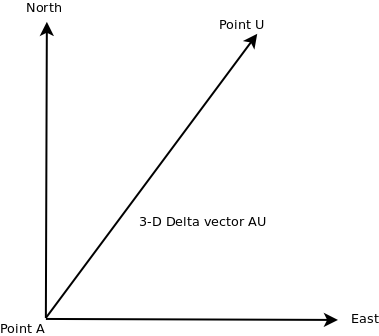
\includegraphics[width=0.4\textwidth]{APdiag1}
\end{center}
\caption{Delta Addition Algorithm}
\label{fig:Delta Addition Algorithm}
\end{figure}

2. \textbf{Azimuth Vector Addition.} Given POS A, distance DIS AU and azimuth AZM AU, simply apply trigonometry and vector addition to get the position of U. Note that the azimuth is signed and always defined as zero at North, increasing toward East, so there is no ambiguity in quadrants.
\begin{figure}[H]
\begin{center}
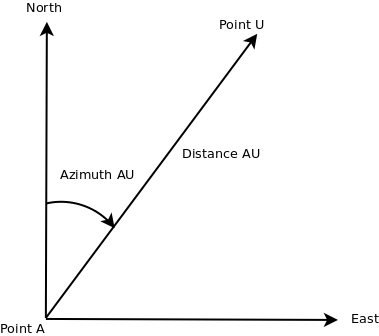
\includegraphics[width=0.4\textwidth]{APdiag2}
\end{center}
\caption{Azimuth Vector Addition Algorithm}
\label{fig:Azimuth Vector Addition Algorithm}
\end{figure}
%             N           U
%             ^          /
%             |         /                U(N) = A(N) + AU*cos(AZM(AU))
%             |        /                 U(E) = A(E) + AU*sin(AZM(AU))
%             |       / DIS AU
%             |AZM AU/
%             |     /
%             |    /
%             |   /
%             |  /
%             | /
%             |/
%             A----------------> E

3. \textbf{Horizontal Angle Vector Addition.} Given POS A and B, DIS AU and horizontal angle HAN(BAU), simply apply trigonometry and vector addition to get the unknown site U. Note that HAN(BAU) is signed.
\begin{figure}[H]
\begin{center}
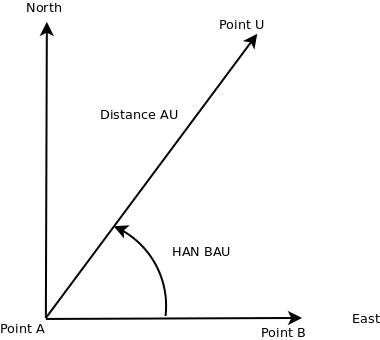
\includegraphics[width=0.4\textwidth]{APdiag3}
\end{center}
\caption{Horizontal Angle Vector Addition Algorithm}
\label{fig:Horizontal Vector Addition Algorithm}
\end{figure}
%             N           U
%             ^          /
%             |         /           Note that a = HAN BAU but must worry about sign
%             |        /                   U(N) = A(N) + AU*sin(a)
%             |       /                    U(E) = A(E) + AU*cos(a)
%             |   AU /
%             |     /
%             |    /
%             |   /
%             |  /
%             | /
%             |/ a
%             A---------------------- B --> E

4. \textbf{Triangulation.} Given POS A and B and a = HAN(UAB) and b = HAN(UBA), the triangle formed by A,B,U has two known angles (a,b) and a known side (AB) between them. The third angle is $c = \pi/2 - a - b$ by identity, and the law of sines will yield the other two sides (DIS AU and BU). Then take distance AU and azimuth AU and use algorithm 2, and do the same for B.
\begin{figure}[H]
\begin{center}
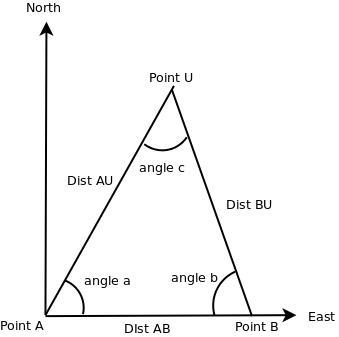
\includegraphics[width=0.4\textwidth]{APdiag4}
\end{center}
\caption{Triangulation Algorithm}
\label{fig:Triangulation Algorithm}
\end{figure}
%             N           U
%             ^          /c\             a+b+c=PI
%             |         /   \            Note that a = |HAN UAB| but
%             |        /     \                     b = |(2PI - HAN ABU)|
%             |       /       \          (interior angles of a triangle always < Pi)
%             |      /         \
%             |     /           \
%             |    /             \
%             |   /               \
%             |  /                 \
%             | /                   \
%             |/a                   b\
%             A---------------------- B --> E

5. \textbf{Two Azimuth Lines.} Given POS A and B and AZM(AU) and AZM(BU), two lines are defined that must meet at a point, which is U. Since A and B are known, DIS(AB) and AZM(AB) can be computed. Solve for U using simple algebra. Note that there are two different ways to collect the AZM(AU): (a) AZM(AU) is found in the measurements and (b) HAN(UAC) and AZM(AC) are found for some POS C (known or not), then HAN(UAC) = AZM(AC) - AZM(AU) (by identity) and therefore AZM(AU) can be computed.
\begin{figure}[H]
\begin{center}
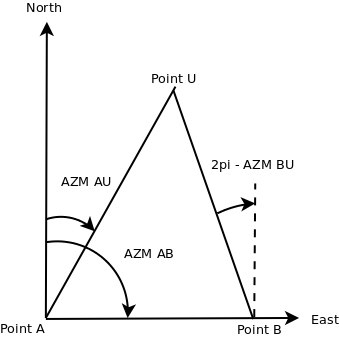
\includegraphics[width=0.4\textwidth]{APdiag5}
\end{center}
\caption{Two Azimuth Lines Algorithm}
\label{fig:Two Azimuth Lines Algorithm}
\end{figure}
%               ^          / \
%               |         /   \
%               |        /     \2pi-azBU|
%               |       /       \       |
%               |      /         \      |
%               |     /           \     |
%               |azAU/             \    |
%               |   /               \   |
%               |  /                 \  |
%               | /                   \ |
%               |/a                   b\|   AZM AB is ~Pi/2 here
%               A---------------------- B --> E
   
6. \textbf{Resection.} Given known POS A, B and C, HAN(AUB) and HAN(BUC), solve for U. This is the 3-point Resection Problem. The algorithm makes use of the fact that for a given HAN(AUB), points A, B and U all lie on a circle. Thus the given data defines two circles that must meet at two points, B and U, and since B is known this uniquely determines U. The implementation must handle the case (called semi-singular) where one of the angles is zero; then the problem reduces to finding the intersection of a circle and a line (e.g. A,D,B,U in figure 4.6, where HAN(AUD) = 0). See figure 4.6, and also figure 4.7, which is a real example from the solver, with the two circles and their origins shown. Ref \cite{ghilani} section 15.5, and \cite{ligas}.
\begin{figure}[H]
\begin{center}
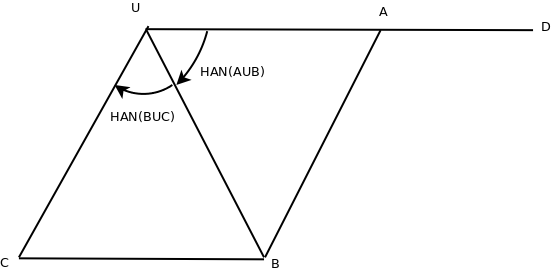
\includegraphics[width=0.6\textwidth]{APdiag7}
\end{center}
\caption{Resection Algorithm}
\label{fig:Resection Algorithm}
\end{figure}

\begin{figure}[H]
\begin{center}
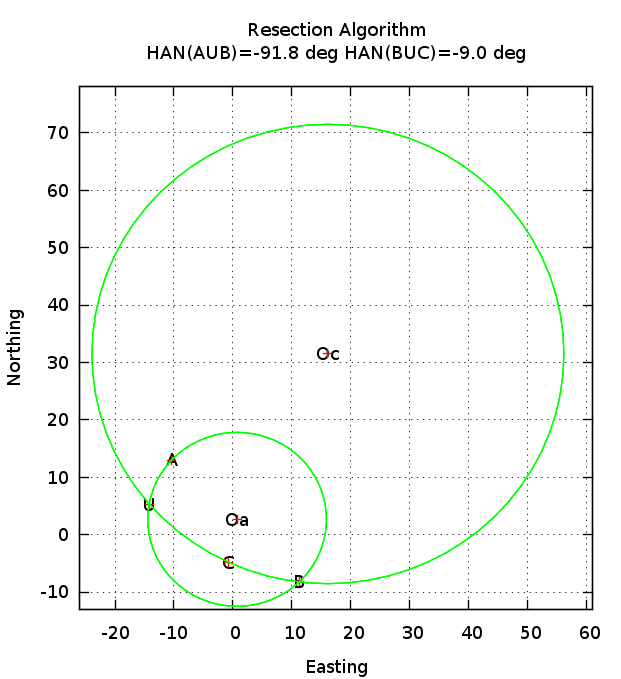
\includegraphics[width=0.6\textwidth]{APdiag6}
\end{center}
\caption{Example of Resection Computation (with circle origins included)}
\label{fig:Example Resection Computation}
\end{figure}
%                           U-----------------------A---------------D
%                          / \ HAN(AUB)            /
%                         /   \                   /
%                        /     \                 /
%                       /       \               /
%                      / HAN(BUC)\             /
%                     /           \           /
%                    /             \         /
%                   /               \       /
%                  /                 \     /
%                 /                   \   /
%                /                     \ /
%               C-----------------------B
%

% TODO \cite{bancroft}
7. \textbf{Ranging.} This algorithm is very similar to the GNSS pseudorange-only navigation solution, and its implementation is based on the Bancroft algebraic solution of GPS ranging. Given 2 or more points and the distances (ranges) from these points to the unknown point, a least squares solution can be formed yielding the position of the unknown. This is a 3-D algorithm; however in this application the positions typically all lie very nearly in a plane. To avoid the near singularity in the height that this produces, the data is transformed to the North-East plane before applying a 2-D algorithm. In every case the algorithm yields two different solutions, but internal consistency allows it to pick the correct one, with one exception. In the case of only 2 positions and distances, the consistency test does not apply, and some other, independent, information must be used to determine the correct solution.

8. \textbf{Leveling Loop Formation.} Any points which remained unsolved after iterating through the previous methods will be inspected to see if they are part of a leveling loop. Iterating through the list of previously known / estimated points, a starting point is gathered. All possible loops with the starting point are formed by chaining together HDIF records using the From and To labels (for more information on HDIF records refer to chapter \ref{chap:LsaRecordGuide}). The loop is considered complete once a point is found whose label does not exist as a From point in the set of HDIF records. At this point a loop from the set is chosen which meets the prioritized conditions below

\begin{enumerate}
	\item The last To station in the chain must be known / estimated.
	\item There are two or more HDIF records in the chain. This prevents the algorithm providing a loop that just connects two known points with no unknown points in the middle.
	\item The loop's distance between the first point and last point is minimized.
	\item If two or more loops have the same distance between their start and end points, the loop with the smallest set of HDIF records is chosen.
\end{enumerate}

Once a loop is chosen all temporary points are evenly spaced on the NE plane between the starting point and the end point. The latitude and longitude for those temporary points are fixed. This process is iterated over until no more points can be projected in this manner.

9. \textbf{Side Shot Handling.} If there remain unknown points after checking for leveling loops, a check for side shots will be performed. This algorithm will search for the following conditions.

\begin{enumerate}
	\item A known / estimated point shares the same label as the From label for an HDIF record.
	\item The To label for that HDIF record corresponds to an unknown point.
\end{enumerate}

If the conditions are met, then the unknown point will have its initial coordinates set equivalent to the known / estimated point. Additionally, its latitude and longitude will be fixed.

10. \textbf{CenterOfMass.} This is the default fall-back; if nothing else can determine the unknown point, then the solver will compute the average of all the known positions (the centroid of the network) and use that for U. This may or may not cause the solver to diverge, depending on the problem, but it probably will lead to the solver requiring a large number of iterations.


\section{How to read the solver output file}
\label{sec:howtoreadoutfile}
This section discusses, in some detail, what is in the solver output file, what is most important there, and how to determine what is wrong when an adjustment computation gives poor results or fails.

\subsection{What is in the solver output file?}
The solver output contains all the information of interest that was either input to, or is produced by the solver, and so it can be quite long. The output is written during the operation of the solver, and falls into 6 basic parts, as follows.

\begin{itemize}
\item Part 1. Input - echo and summarize input from both DAT file and command line
\item Part 2. Compute \emph{a priori} positions, if needed
\item Part 3. Load the geoid file and define constraints, if any
\item Part 4. Build the LS problem and print the degrees of freedom, etc.
\item Part 5. Results for each iteration (this is the largest part of the output: convergence test, data residuals and diagnostics at every iteration)
\item Part 6. Final results - residuals, statistical tests, adjustments, and geoid calculations.
\end{itemize}

The input section includes all the data and positions, just as they are in the input. Any errors encountered in reading the DAT file are shown here as ``Error - DAT reader failed to parse line $>...<$''; however the solver will NOT quit. Note that the solver might terminate after part 2, either because it was unable to find all the \emph{a priori} positions, or because the user requested it from the command line.

Part 4 is very brief and shows the number of degrees of freedom, the size of the state and data vectors, the number of constraints, and all the \emph{a priori} positions. The solver might terminate here if the problem is underdetermined or singular, because then there is no solution.

Part 5 (once per iteration) first shows the convergence test, which indicates how the iteration is proceeding. This is followed by the RMS residuals and the APV. (The same information appears at the command line when the ``progress'' option is used.) Then (if the verbose option is on) the current adjustments with their uncertainties, and a table of all the data residuals, follow; the bulk of this information is not particularly interesting unless there is a problem.

The final part is of most interest. It includes all the data residuals, with standard residuals (these are not in the per-iteration results), final RMS residuals, APV and the Chi-squared tests. Then the final adjustments are presented, both in ECEF XYZ and in Latitude, Longitude and Height. If a geoid file was input, the geoid is evaluated at all the sites as well.

\subsection{What is important?}
Some of the information in the solver output file is much more important than the rest, but this importance can depend on the outcome of the algorithm. The following is a list of things to look for, in order of importance; however note that there is nothing absolute or mandatory about this list - it is really just an informal attempt by the developer to tell the user what to look for, and in what order, in the solver output.

\textbf{1. Errors.} Any fatal error (meaning the solver cannot go on) produces a line in the output that begins with the word ``Error''. Because the solver aborts, this message is probably near the bottom of the output file. These are critical, far more important than anything else in the output file. A normal solver output will not have any Error messages, but if the solver failed for any reason, there will be one. These can be as simple as ``Error - input file not found'' or as complex as ``Error - the problem is singular.'' (Failing to parse a record the DAT file is also an Error; these appear at the top of the output file and do not cause an abort.)

[Note. If the user ever encounters a case where the solver fails, perhaps with ``Exception: ...'' and no Error message is found, please report this to the developers, and send along the DAT file.]

\textbf{2. Warnings.} An error that is not fatal, but that is not expected and of concern, produces a line in the output that begins with the word ``Warning.'' Many solver runs will produce no Warnings. Some will point out problems that cause the user to make changes to the input and re-run the solver, but some may be ignored. These should at least be considered before going on; most are the result of problems or omissions in the input.

Probably the most common are the Warnings about ``unused positions'' and ``unused data.'' If any site (POS record) is given in the input, but then that site is never used in the data, that site's name is listed as an unused position. Likewise if there is a data record that involves only fixed sites, it cannot be used in the estimation, and so it is an unused datum. Unused positions are innocuous, they are not used by the solver but are echoed in the final output, and some users don't mind having them in the output. Unused data, however, is probably an oversight, perhaps because the wrong sites are used, or some sites are mistakenly fixed.

\textbf{3. Statistics.} In the absence of Errors and serious Warnings, next look at the post-fit residuals RMS and the APV. Search for the word ``Final'' or ``APV'' to find these values, which are below the final data residuals and before the final adjustments. An example from a solver run:

\begin{Snippet}
 RMS post-fit relative residual (Final) = 8.251e-01
 Degrees of freedom = 50; Std dev of unit weight = 1.161; APV = 1.348 (Final)
 RMS post-fit raw residual (angles) (Final) = 9.600e-05 rad = 1.980e+01 soa.
 RMS post-fit raw residual (length) (Final) = 4.060e-03 m.
 Upper Chi-squared test (0.950): 1.35 < 1.35 pass
 Lower Chi-squared test (0.050): 0.70 < 1.35 pass
 Two-sided Chi-squared test (0.025,0.975): 0.647 < 1.348 < 1.428 pass
\end{Snippet}

The example output shows the post-fit residual RMS (relative, angles, and lengths), the APV, and the Chi-squared (though actually the APV) test results. The post-fit residual RMS provides a sense of how well the newly estimated states fit the measurements; the relative residuals are the raw post-fit residuals scaled by the associated specified measurement uncertainty, and thus the RMS of the relative residuals provides an indication of the how well the provided measurement uncertainties match the actual noise of the measurements. 

The ``Chi-squared test'' is actually a test of the APV value, because the solver outputs limits for this test equal to the $\chi^2$ limits for a particular confidence value, divided by the system degrees of freedom, and thus the limits have the same form as the APV value. The optimum value for the APV is 1.0, indicating the noise seen in the post-fit residuals matches well with the provided measurement uncertainties. If the APV is well over 1.0, the post-fit residuals variance greatly exceeds the provided measurement uncertainties, and vice versa for APV values well under 1.0. 

\textbf{4. How to interpret the ``Chi-squared'' test.} If the solution fails the upper ``Chi-squared'' test (i.e. the APV is well over 1.0), the post-fit residuals distribution is much larger than the provided measurement uncertainties and the results should be analyzed for possible blunders (see below). If the user is confident there are unlikely any blunders and the APV still exceeds the upper test value, the overall scale of the uncertainties may be too low, and the user may want to increase some measurement uncertainties to move the APV closer to 1.0.

Note that while the user can always make the APV exactly 1.0 by rescaling the entire measurement covariance matrix, this scaling has no effect on the solution (see section \ref{sect:BasicLeastSquares}). Rather than scaling the entire measurement covariance, the user may want to look for any subsets of the data that have larger noise than expected (as determined by considering relative or standard residuals), and scale up the provided measurement uncertainties for those particular measurements. Changing only a subset of the measurement uncertainties changes the relative weighting of the measurements in the least squares method, and thus the solution is impacted (and if done properly, improved).

If the solution fails the lower ``Chi-squared'' test (i.e. the APV is well under 1.0), the post-fit residuals distribution is much smaller than the provided measurement uncertainties. In this case, the user may wish to look for any subsets of the data that have smaller noise than expected (as determined by considering relative or standard residuals), and scale down the provided measurement uncertainties for those particular measurements. The solution will be improved if the scaling is done properly. However, the risk of having a non-optimal solution when the APV is very small is lower as compared to when the APV is very large, so the user may wish to skip this scaling down step if time is tight. 

Finally, to quote Ghilani (\cite{ghilani} p. 529): ``[the chi-squared test does not] reveal the exact problem in data when the test fails. The chi-sqared test should be viewed as a warning flag for an adjustment that requires further analysis''.

\textbf{5. Blunders.} Now the user should look at the ``Data and residuals (Final)'' table, particularly to look for any potential remaining blunders. The table has in the right-most two columns the redundancy and the standard residual for each measurement, both of which are derived in appendix \ref{appendices:RedStdResComp}. In a nutshell, the redundancy is a number between 0 and 1 that indicates how susceptible the solution is to errors in that observation, and the standard residual is a further ``normalization'' of the relative residual involving the APV and the redundancy of the measurement. The redundancy indicates whether more observations are needed to safeguard against blunders in a particular observation. The standard residual provides an indication of whether the measurement is erroneous, unreasonable, or problematic (e.g. from a user blunder). The process of reviewing the standard residuals and removing or correcting any problematic observations is often called ``data snooping'' in the literature. 

Any observations that exceed a threshold based on the tau distribution, as described in appendix \ref{appendices:RedStdResComp}, are marked with two asterisks: ``**''. For convenience, the three lines with the largest standard residuals are repeated in the subsequent table ``Largest 3 standard residuals''. The user may wish to check each of these marked observations for blunders, with a focus on the data and/or sites involved in that measurement. Note that one blunder can affect many other quantities in the adjustment (estimated states and post-fit residuals), so we strongly encourage the user to look for and correct only one blunder at a time, starting with the largest (likely associated with the largest standard residual). After fixing that largest blunder, re-run the adjustment and consider if there are any further blunders via another review of the standard residuals.

\textbf{6. Adjustments.} Finally, consider the adjustment (or ``update'') state vector and final adjusted positions. All final positions (adjusted, fixed, and unused), along with their associated adjustment vector and formal covariance (for adjusted positions), are provided in three tables corresponding to three different coordinates: ``Final Adjusted Positions XYZ'' (for the positions in ECEF), ``Final Adjusted Positions LLH'' (for the positions in geodetic latitude, longitude, and height above the WGS-84 ellipsoid), and ``Final Adjusted Positions Astronomic'' (for the positions in astronomic coordinates, along with deflection and undulation values, which required a geoid file be loaded).

\section{Solution Methods}
There are many ways to solve the least squares problem. These methods can be slow or fast,
robust or unstable \textemdash \ in many cases these properties depend on the nature of the problem.
The system of equations for survey adjustments tends to be very large 
and sparse; that is, there are many unknown states and mostly zero terms in 
the problem. As a result, the system matrix tends to be large, and
the computation time for traditional methods generally increases exponentially 
with size.

However, since the system matrix is generally sparse, a huge performance
gain can be obtained by cleverly performing operations only on the 
non-zero elements. \textsf{lsasolver} offers two different
methods to obtain the solution, both of which leverage sparse matrix 
strategies to minimize computation time.

\subsection{Square Root Information Filter}
The Square Root Information Filter (SRIF) uses the Householder method
mentioned in Section \ref{sec:nonlinsolver} and is considered to be extremely robust \cite{biermann}.
SRIF is notable in that the problem is not squared, the usual operation used 
to project the data onto the column space of the system matrix. 
In general, it is not desirable to square the problem since this 
reduces the space of the numeric precision and can lead to instability 
for poorly conditioned problems.

Another key feature of the SRIF is that this method allows for
easy determination of certain properties such as the presence and 
location of a singularity, the condition number, and the presence of
non-positive eigenvalues without needing to perform another 
computationally expensive operation. However, this is not the fastest available method and the
computation time can be long for large problems. Yet, this method will
produce the most reliable answer and also provides the user with some
additional information which may be helpful in diagnosing issues.

\subsection{Conjugate Gradient Method}
The Conjugate Gradient (CG) method is a departure from the traditional
method of factoring the system matrix. Instead, the CG method reduces
the system of equations to a multidimensional optimization problem. The quadratic
form of the problem is represented as the following:
\begin{equation}
f(x) = \frac{1}{2}x^TAx - b^Tx
\end{equation}
This function represents a multidimensional quadratic which may have
a minimum or maximum, depending on whether the system is positive- 
or negative-definite. The critical point of this function occurs where
its gradient is equal to zero:
\begin{equation}
(\nabla f)^T = \frac{1}{2}(A^T + A)x - b = 0
\end{equation}
It can be seen that if A is symmetric, this reduces to:
\begin{equation}
(\nabla f)^T = Ax - b
\end{equation}
Thus, a converging solution (i.e. one in which the residuals are minimized) to the problem $x$ can be determined by minimizing $f(x)$ if and
only if A is symmetric and positive-definite. \\ \\
The current implementation of this method squares the system matrix which
reduces the precision of the solution relative to the SRIF formulation.
The following is a representation of the weighted, squared problem:

\begin{equation}
\begin{split}
Ax &= b \\
& \Downarrow \\ 
A^TWAx &= A^TWb
\end{split}
\end{equation}

Since the problem was reduced from a factoring operation to an optimization
process, the time per iteration of the non-linear problem is greatly reduced.

Instead of building a custom CG implemenation for \textsf{lsasolver},
the Eigen library is used to perform this operation \cite{eigenweb}. The 
Eigen library also utilizes many optimizations depending on the
type of matrix used and the matrix operation.

\subsection{What is the best method?}
The default behavior of \textsf{salsa} is to try to use the CG method (because it is very fast)
 and fall back to the SRIF only if an error is detected. In general, the CG method will produce
a solution that is equally useful (i.e. precise far beyond significant figures),
but there may be some information lost if there are issues or the problem
diverges.

The user may specity which solver method(s) will be applied by \textsf{lsasolver}.  Under \textsf{salsa}'s project configuration options (\texttt{Project} $\to$ \texttt{Configure\ldots}), the user may choose one of three options under ``Performance optimization:''
\begin{description}
\item[Allow fast] With this option specified, \textsf{salsa} will invoke \textsf{lsasolver} with the command-line argument \verb+--forcefast+. If the fast (CG) method fails, \textsf{salsa} will try again, this time calling \textsf{lsasolver} with the \verb+--forcestable+ argument.  This process will typically be transparent to the user and is the recommended default behavior.
\item[Force fast] With this option specified, \textsf{salsa} will invoke \textsf{lsasolver} with the command-line argument \verb+--forcefast+.  If that fails, an error message will be returned to the user.  This option may be appealing when the survey network is very large, and the delay in returning a result with the SRIF implementation is unacceptable.
\item[Force stable] With this option specified, \textsf{salsa} will invoke \textsf{lsasolver} with the command-line argument \verb+--forcestable+.  This option may be appealing when the network is unstable, and the diagnostic output from the SRIF implementation is helpful in diagnosing the issue.  For example, if a position in the network lacks any measurement data to determine the point's height, the CG method may simply fail, whereas the SRIF method may be able to report that the problem is singular, at that specific point.
\end{description}

\section{Example 0: GPS Only}

To help the user understand what outputs are displayed on the screen after calculating an adjustment, we will begin by considering a simple example which reduces to a two dimensional problem.  The purpose of this example is to explicitly show how the \textsf{salsa} outputs are computed.  To aide with visualizing this example, Figure \ref{fig:ex0} presents the final adjusted network that we will obtain.  To follow along, copy and paste the \verb+example00+ folder to your desktop.  Launch \textsf{salsa} and select Project $\ra$ Open LSA and select \verb+ex0.proj+ from inside of the \verb+example00+ folder.  Next, we will ensure that reliability calculations are enabled for this project. Reliability metrics are a helpful tool to diagnose the network's susceptibility to blunders and are are given in-depth coverage in example 2 and appendix \ref{appendices:RedStdResComp}. Reliability metrics are enabled by default so the user should not have to change any settings to perform these calculations. However, if reliability metrics are not enabled, the following instructions will allow the user to enable them. To enable reliability calculations, open the Configuration Menu by selecting the menu action Project $\to$ Configure\ldots and under the Solver Options box, select the \verb+yes+ button next to Calculate External Reliability. Press \verb+OK+ at the bottom of the Configuration Menu to accept the changes and close the window. To see the final adjusted result select Project $\ra$ Calculate Adjustment.  Interaction with the \textsf{salsa} interface will be covered in much greater detail in example 1 in chapter \ref{chap:examples}.

\begin{figure}[!htbp]
\begin{center}
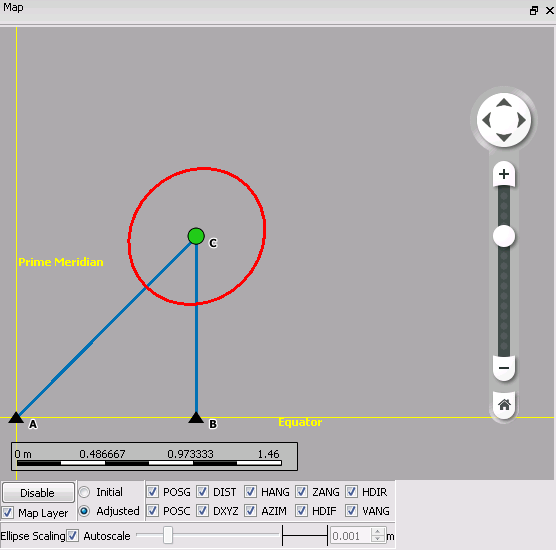
\includegraphics[width=0.7\textwidth]{example0/networkdesign.png}
\end{center}
\caption{Example 0 network.}
\label{fig:ex0}
\end{figure}

We will place one control station (A) at $0^o$ latitude, $0^o$ longitude and $0$ m height.  We will place a second control station (B) about a meter away at $0^o$ latitude, $(-9\times10^{-6})^o$ W longitude and $0$ m height.  The control station coordinates are presented in Table \ref{tab:ex0_ctrl}

\begin{table}[htb]
\caption{Example $0$ Control Network}
\label{tab:ex0_ctrl}
\begin{center}
\begin{tabular}{lrrr}
\hline
\textbf{Site} & \textbf{Latitude} & \textbf{Longitude} & \textbf{Height} \\
\hline
A & $0^o$ N & $0^o$ W & $0$ m \\
B & $0^o$ N & $(-9\times10^{-6})^o$ W & $0$ m \\
\hline
\end{tabular}
\end{center}
\end{table}

The GPS measurement data from control station (A) to the floating point (C) is entered into \textsf{salsa} in ECEF coordinates as ($0$ m, $1$ m, $1$ m).  The GPS measurement data from control station (B) to the floating point (C) is ($0$ m, $0$ m, $1$ m).  Associated with these measurements is an uncertainty which is entered as a covariance matrix.  For simplicity, we will choose both sets of measurements to have the same covariance matrix.  The GPS measurements and the measurement covariance matricies are presented in Table \ref{tab:ex0M}.

\begin{table}[htb]
\caption{Example $0$ Measurements}
\label{tab:ex0M}
\begin{center}
\begin{tabular}{ccccc}
\hline
\textbf{From-To}&\textbf{$\mathbf{\Delta}$X(m)\hspace*{3mm}$\mathbf{\Delta}$Y(m)\hspace*{3mm}$\mathbf{\Delta}$Z(m)}&\textbf{Q$_{\textbf{XX}}$(m$^2$)}&\textbf{Q$_{\textbf{XY}}$(m$^2$)}&\textbf{Q$_{\textbf{XZ}}$(m$^2$)}\\
&&\textbf{Q$_{\textbf{YY}}$(m$^2$)}&\textbf{Q$_{\textbf{YZ}}$(m$^2$)}&\textbf{Q$_{\textbf{ZZ}}$(m$^2$)}\\
\hline
A-C & $0$\hspace*{12mm}$1$\hspace*{12mm}$1$ &$10^{-12}$&$10^{-12}$&$10^{-12}$\\
    &           &$10^{-6}$&$10^{-7}$&$10^{-6}$\\
B-C & $0$\hspace*{12mm}$0$\hspace*{12mm}$1$ &$10^{-12}$&$10^{-12}$&$10^{-12}$\\
    &           &$10^{-6}$&$10^{-7}$&$10^{-6}$\\
\hline
\end{tabular}
\end{center}
\end{table}

There are in principle six observation equations, one for each measurement.  However, to simplify the presentation we will neglect the observation equations corresponding to the X coordinate in the ECEF frame (U in the ENU frame).  This is valid because the displacements and covariances have been artificially chosen such that the neglected axis does not significantly influence the result for the other two axes.  Denoting the residuals by $R$, the observation equations for our effective 2D system are
\begin{equation}
\begin{array}{c}
\text{R}_{\text{Y}_{\text{CA}}}=-\text{Y}_{\text{C}}+\left(\text{Y}_{\text{C}}+\Delta\text{Y}_{\text{CA}}\right)\\
\text{R}_{\text{Z}_{\text{CA}}}=-\text{Z}_{\text{C}}+\left(\text{Z}_{\text{C}}+\Delta\text{Z}_{\text{CA}}\right)\\
\text{R}_{\text{Y}_{\text{CB}}}=-\text{Y}_{\text{C}}+\left(\text{Y}_{\text{C}}+\Delta\text{Y}_{\text{CB}}\right)\\
\text{R}_{\text{Z}_{\text{CB}}}=-\text{Z}_{\text{C}}+\left(\text{Z}_{\text{C}}+\Delta\text{Z}_{\text{CB}}\right)
\end{array}\ra\mathop{\underbrace{\left[\begin{array}{c}\text{R}_{\text{Y}_{\text{CA}}}\\\text{R}_{\text{Z}_{\text{CA}}}\\\text{R}_{\text{Y}_{\text{CB}}}\\\text{R}_{\text{Z}_{\text{CB}}}\end{array}\right]}_{\ds{\mathbf{R}}}}=-\mathop{\underbrace{\left[\begin{array}{cc}1&0\\0&1\\1&0\\0&1\end{array}\right]}_{\ds{\mathbf{P}}}}\cdot\mathop{\underbrace{\left[\begin{array}{c}\text{Y}_{\text{C}}\\\text{Z}_{\text{C}}\end{array}\right]}_{\ds{\mathbf{X}}}}+\mathop{\underbrace{\left[\begin{array}{c}\text{Y}_{\text{A}}+\Delta\text{Y}_{\text{CA}}\\\text{Z}_{\text{A}}+\Delta\text{Z}_{\text{CA}}\\\text{Y}_{\text{B}}+\Delta\text{Y}_{\text{CB}}\\\text{Z}_{\text{B}}+\Delta\text{Z}_{\text{CB}}\end{array}\right]}_{\ds{\mathbf{d}}}}.
\end{equation}
We have rewritten the observation equations in matrix form by introducing the residual vector $(\mathbf{R})$, the partials matrix $(\mathbf{P})$, the state vector $(\mathbf{X})$ and the data vector $(\mathbf{d})$.

The approach of least squares analysis allows us to find the most probable state vector $(\mathbf{X})$ by minimizing a constructed quantity which is a sum of residuals squared.  The quantity we minimize knows about the measurement uncertainties and uses those to weight the terms in the sum (i.e. minimize $\Sigma$(weight)$\text{R}^2$).  The weight matrix ($\mathbf{W}$) is given by the inverse of the measurement covariance matrix ($\mathbf{MCov}$)
\begin{equation}
\mathbf{W}=\mathbf{MCov}^{-1}=\left[\begin{array}{cccc}10^{-6}&10^{-7}&0&0\\10^{-7}&10^{-6}&0&0\\0&0&10^{-6}&10^{-7}\\0&0&10^{-7}&10^{-6}\end{array}\right]^{-1}\text{m}^{-2}=\left[\begin{array}{cccc}10^6&-10^5&0&0\\-10^5&10^6&0&0\\0&0&10^6&-10^5\\0&0&-10^5&10^6\end{array}\right]\text{m}^{-2}.
\end{equation}
The quantity to be minimized is
\begin{equation}
\mathbf{R}^T\cdot\mathbf{W}\cdot\mathbf{R}=(\mathbf{P}\cdot\mathbf{X}-\mathbf{d})^T\cdot\mathbf{W}\cdot(\mathbf{P}\cdot\mathbf{X}-\mathbf{d}).
\end{equation}
The superscript $T$ denotes the transpose operation.  To proceed with the minimization, the quantity is differentiated with respect to the state vector $\mathbf{X}$.  This results in the equation for the state vector introduced in the previous Chapter
\begin{equation}
\mathop{\underbrace{(\mathbf{P}^T\cdot\mathbf{W}\cdot\mathbf{P})}_{\ds{\mathbf{Cov}^{-1}}}}\cdot\mathbf{X}=\mathbf{P}^T\cdot\mathbf{W}\cdot\mathbf{d}\hspace*{8mm}\ra\hspace*{8mm}\mathbf{X}=\mathbf{Cov}\cdot\mathbf{P}^T\cdot\mathbf{W}\cdot\mathbf{d}.
\end{equation}
Note that the solution covariance ($\mathbf{Cov}$) is given by
\begin{eqnarray}
\mathbf{Cov}&=&(\mathbf{P}^T\cdot\mathbf{W}\cdot\mathbf{P})^{-1}\\
&=&\left(\left[\begin{array}{cccc}1&0&1&0\\0&1&0&1\end{array}\right]\cdot\left[\begin{array}{cccc}10^6&-10^5&0&0\\-10^5&10^6&0&0\\0&0&10^6&-10^5\\0&0&-10^5&10^6\end{array}\right]\cdot\left[\begin{array}{cc}1&0\\0&1\\1&0\\0&1\end{array}\right]\right)^{-1}\text{m}^2\\
&=&\left(2\times\left[\begin{array}{cc}10^6&-10^5\\-10^5&10^6\end{array}\right]\right)^{-1}\text{m}^2=5\times\left[\begin{array}{cc}10^{-7}&10^{-8}\\10^{-8}&10^{-7}\end{array}\right]\text{m}^2.
\end{eqnarray}

With our example we may explicitly write out the state vector
\begin{equation}
\begin{split}
\mathbf{X}&=5\times\left[\begin{array}{cc}10^{-7}&10^{-8}\\10^{-8}&10^{-7}\end{array}\right]\cdot\left[\begin{array}{cccc}1&0&1&0\\0&1&0&1\end{array}\right]\cdot \left[\begin{array}{cccc}10^6&-10^5&0&0\\-10^5&10^6&0&0\\0&0&10^6&-10^5\\0&0&-10^5&10^6\end{array}\right]\cdot\left[\begin{array}{c}1\\1\\1\\1\end{array}\right]\text{m}\\
&=\left[\begin{array}{c}1\\1\end{array}\right]\text{m}
\end{split}
\end{equation}
The residuals are given by
\begin{equation}
\mathbf{R}=-\mathbf{P}\cdot\mathbf{X}+\mathbf{d}\approx-\left[\begin{array}{cc}1&0\\0&1\\1&0\\0&1\end{array}\right]\cdot\left[\begin{array}{c}1\\1\end{array}\right]\text{m}+\left[\begin{array}{c}1\\1\\1\\1\end{array}\right]\text{m}\stackrel{\text{(More precision kept)}}{\approx}\left[\begin{array}{c}-10^{-3}\\-10^{-9}\\10^{-3}\\-10^{-9}\end{array}\right]\text{m}.
\end{equation}
{\color{red}{\textbf{These values are reported under $|$Raw$|$ in the Measurement Residuals table.}}}\\
In the rightmost column we have written the residuals found if one carries more digits of precision through the computation.

Note that this entire process can be repeated until the adjustment size at an iteration is very small (i.e. $\Delta\mathbf{X}$ is below some limit in meters after rewriting $\mathbf{X}=\mathbf{X}_{\text{previous}}+\Delta\mathbf{X}$ and repeating the process to solve for $\Delta\mathbf{X}$).  The covergence value displayed under the heading ``Convergence Test'' is the root-mean-square (RMS) of the adjustment to each floating site coordinate ($\Delta\text{X}^{\text{RMS}}$).  For this simple example the convergence test immediately passes, though the convergence criteria may be modified under Project $\ra$ Configure\ldots if desired.

We have just computed the residuals which populate the $|$Raw$|$ column of the Measurement Residuals table depicted in Figure \ref{fig:ex0gui}.  We will now present how to obtain the remaining outputs which appear in the Measurement Residuals table and the Point Confidence Regions table.

\begin{figure}[!htbp]
\begin{center}
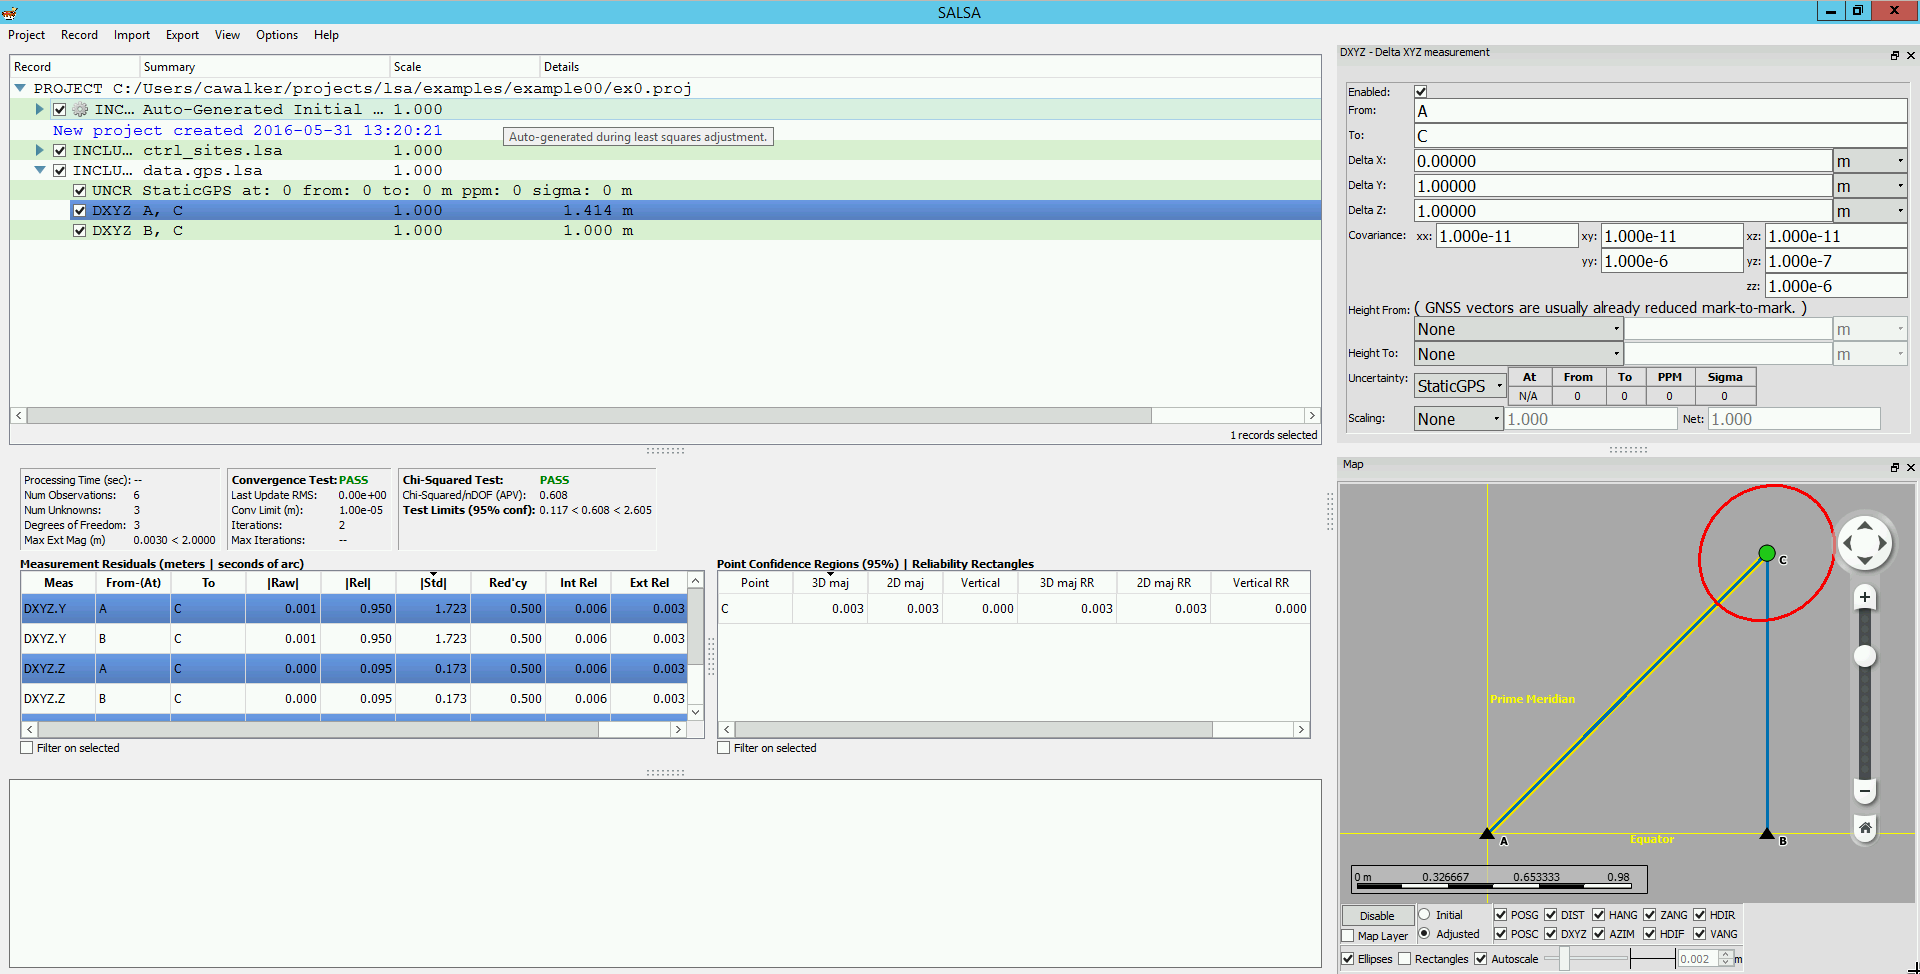
\includegraphics[width=1.0\textwidth]{example0/full.png}
\end{center}
\caption{\textsf{salsa} interface after calculating adjustment with example $0$ data.  This section describes how to compute the output quantities appearing in the output tables.}
\label{fig:ex0gui}
\end{figure}

The next column in the Measurement Residuals table is the Relative Residual.  The intuition for this quantity is that it is the size of the residual for a given measurement divided by the measurement uncertainty (i.e. $\sim\text{R}_i$/uncertainty).  However, since the measurement covariance matrix ($\mathbf{MCov}$) contains off-diagonal terms we must be careful about how we define scaling by (1/uncertainty).  The notation of the ``square root'' of the covariance matrix will take the form of a Cholesky decomposition in which the measurement covariance matrix ($\mathbf{MCov}$) is given as the product of a lower triangular matrix ($\mathbf{L}$) and its transpose ($\mathbf{MCov}=\mathbf{L}\cdot\mathbf{L}^T$),
\begin{equation}
\begin{split}
&\mathop{\underbrace{\left[\begin{array}{cccc}10^{-6}&10^{-7}&0&0\\10^{-7}&10^{-6}&0&0\\0&0&10^{-6}&10^{-7}\\0&0&10^{-7}&10^{-6}\end{array}\right]\text{m}^2}_{\ds{\mathbf{MCov}}}}\\
&=\mathop{\underbrace{\left[\begin{array}{cccc}10^{-3}&0&0&0\\10^{-4}&10^{-3}&0&0\\0&0&10^{-3}&0\\0&0&10^{-4}&10^{-3}\end{array}\right]\text{m}}_{\ds{\mathbf{L}}}}\cdot\mathop{\underbrace{\left[\begin{array}{cccc}10^{-3}&10^{-4}&0&0\\0&10^{-3}&0&0\\0&0&10^{-3}&10^{-4}\\0&0&0&10^{-3}\end{array}\right]\text{m}}_{\ds{\mathbf{L}^T}}}
\end{split}
\end{equation}
The notion of ``division'' is implemented by multiplying with the inverse matrix ($\mathbf{R}_{\text{Rel}}=\mathbf{L}^{-1}\cdot\mathbf{R}$)
\begin{equation}
\begin{split}
\mathbf{R}_{\text{Rel}}&=\mathop{\underbrace{\left[\begin{array}{cccc}10^{-3}&0&0&0\\10^{-4}&10^{-3}&0&0\\0&0&10^{-3}&0\\0&0&10^{-4}&10^{-3}\end{array}\right]^{-1}\text{m}^{-1}}_{\ds{\mathbf{L}^{-1}}}}\cdot\mathop{\underbrace{\left[\begin{array}{c}-10^{-3}\\-10^{-9}\\10^{-3}\\-10^{-9}\end{array}\right]\text{m}}_{\ds{\mathbf{R}}}} \\
&\stackrel{\text{(More precision kept)}}{\approx}\left[\begin{array}{c}-0.95\\0.095\\0.95\\-0.095\end{array}\right]
\end{split}
\end{equation}
{\color{red}{\textbf{These values are reported under $|$Rel$|$ in the Measurement Residuals table.}}}\\
We again have presented the final result if one keeps more digits of precision.  Note the relative residual has been defined such that it is dimensionless.

Before computing the standard residual, we need to introduce the concept of a posteriori variance (APV).  Considerations relating to APV requires that we treat the full 3D nature of our problem since the number of observations is different which influences the root-mean-square that we will compute shortly.  APV is the $\chi^2$ value divided by the number of degrees of freedom.  Above the Measurements Residuals table the number of observation equations ($n_{\text{eq}}$) and the number of variables ($n_{\text{var}}$) are given, the difference between these two is displayed as the degrees of freedom ($n_{\text{dof}}=n_{\text{eq}}-n_{\text{var}}=6-3=3$).  The $\chi^2$ value depends on the RMS of the relative residuals
\begin{equation}
\begin{split}
\text{R}_{\text{Rel}}^{\text{RMS}}&=\sqrt{\f{1}{n_{\text{eq}}}\left(\Sigma_{i=1}^{n_{\text{eq}}}\text{R}_{\text{Rel},i}^2\right)}\\
&=\sqrt{\f{1}{6}\left[0+(0.95)^2+(0.095)^2+0+(0.95)^2+(0.095)^2\right]}=0.55.
\end{split}
\end{equation}
Note that the $\text{X}_{\text{ECEF}}$ component contributes negligibly to the sum, but the presence of the two $\text{X}$ component observations changes the divisor under the square root.  The value of $\chi^2$ is given by square of the previously computed RMS times the number of equations ($\chi^2=(\text{R}_{\text{Rel}}^{\text{RMS}})^2\cdot n_{\text{eq}}$).  The APV is the $\chi^2$ per degree of freedom
\begin{equation}
\text{APV}=\f{\chi^2}{n_{\text{dof}}}=\left(\text{R}_{\text{Rel}}^{\text{RMS}}\right)^2\cdot\left(\f{n_{\text{eq}}}{n_{\text{dof}}}\right)=(0.55)^2\cdot\left(\f{6}{3}\right)=0.6.
\end{equation}
{\color{red}{\textbf{This value is reported as APV under the ``Chi-Squared Test'' heading.}}}\\

The ``Chi-Squared Test'' heading will display ``PASS'' if the APV is within an interval indicated next to the ``Chi-Squared:'' text above the Point Confidence Regions table.  The interval that the APV must lie in is set by the number of degrees of freedom and the desired confidence level.  The values are determined by the $\chi^2$ percent point function (ppf).\footnote{Unfortunately, a nice analytical formula for the ppf does not exist.  However, many languages support computation of the ppf.  For instance, in Python one may use the command ``chi2.ppf(cf,ndof)'' after importing ``from scipy.stats import chi2''.}  The $\chi^2$ ppf is the inverse of the cumulative distribution function (cdf)
\begin{equation}
\text{ppf}_{\chi^2}(c_f,n_{\text{dof}})=\chi^2\text{ such that }\text{cdf}_{\chi^2}(\chi^2,n_{\text{dof}})=c_f,\text{ where }\text{cdf}_{\chi^2}(c_f,n_{\text{dof}})=\f{\gamma_{\text{inc}}\left(\f{n_{\text{dof}}}{2},\f{c_f}{2}\right)}{\Gamma\left(\f{n_{\text{dof}}}{2}\right)}.
\end{equation}
Here $c_f$ denotes a confidence factor dependence on the desired confidence level ($c$), $\Gamma$ denotes the usual Gamma function and $\gamma_{\text{inc}}$ denotes the lower incomplete Gamma function.  The APV lower bound is determined by evaluating the $\chi^2$ ppf with the confidence factor equal to $c_{f,\text{lower}}=(1-c)$ and dividing by $n_{\text{dof}}$.  Likewise, the APV upper bound is determined by letting $c_{f,\text{upper}}=c$ in ppf$_{\chi^2}$ and dividing by $n_{\text{dof}}$.  In our example, chi2.ppf(1-0.95,3)/3=0.117 (95\% probability to obtain an APV$\geq0.117$) and chi2.ppf(0.95,3)/3=2.605 (95\% probability to obtain an APV$\leq$2.605).  The .out file lists intervals for other values of $c_f$.  You can adjust the $c_f$ used for the interval displayed in the GUI under Project $\ra$ Configure\ldots

The standard residuals are the relative residuals rescaled by the APV and the redundancy
\begin{equation}
\mathbf{R}_{\text{std}}=\left[\begin{array}{c}\text{R}_{\text{Rel},1}/\sqrt{\text{APV}\cdot\text{Rd}_1}\\\text{R}_{\text{Rel},2}/\sqrt{\text{APV}\cdot\text{Rd}_2}\\\text{R}_{\text{Rel},3}/\sqrt{\text{APV}\cdot\text{Rd}_3}\\\text{R}_{\text{Rel},4}/\sqrt{\text{APV}\cdot\text{Rd}_4}\end{array}\right]=\left[\begin{array}{c}-1.7\\0.17\\1.7\\-0.17\end{array}\right].
\end{equation}
{\color{red}{\textbf{These values are reported under $|$Std$|$ in the Measurement Residuals table.}}}\\
When the standard residual exceeds a threshold based on a particular confidence value, as described in appendix \ref{appendices:RedStdResComp}, that measurement may be a blunder.

The redundancy number for a particular observation is a measure of how well blunders can be detected and resolved within a set of observations.  A low redundancy may imply that there is not a sufficient number of observations to determine if a blunder is present. The effects of low redundancy can be explicitly defined using reliability metrics, which are shown in the remaining columns in the Measurement Residuals table. Considerable attention is given to reliability metrics and their uses in example 2. For a complete mathematical introduction to reliability metrics please reference appendix \ref{appendices:RedStdResComp}. 

The redundancy number depends on the residual covariance matrix ($\mathbf{Q}_{\text{RR}}$) which is the difference of the measurement covariance matrix ($\mathbf{MCov}$) and the inverse of the weight matrix as estimated by the solution covariance matrix ($\mathbf{Cov}$)
\begin{equation}
\mathbf{W}^{-1}_{\text{estimated}}=\mathbf{P}\cdot(\mathbf{P}^T\cdot\mathbf{W}\cdot\mathbf{P})^{-1}\cdot\mathbf{P}^T=\mathbf{P}\cdot\mathbf{Cov}\cdot\mathbf{P}^T.
\end{equation}
The residual covariance matrix is therefore explicitly given as ($\mathbf{Q}_{\text{RR}}=\mathbf{MCov}-\mathbf{W}_{\text{estimated}}^{-1}$)
\begin{equation}
\begin{split}
\mathbf{Q}_{\text{RR}} &= \mathop{\underbrace{\left[\begin{array}{cccc}10^{-6}&10^{-7}&0&0\\10^{-7}&10^{-6}&0&0\\0&0&10^{-6}&10^{-7}\\0&0&10^{-7}&10^{-6}\end{array}\right]\text{m}^2}_{\ds{\mathbf{MCov}}}}-\mathop{\underbrace{\left[\begin{array}{cc}1&0\\0&1\\1&0\\0&1\end{array}\right]}_{\ds{\mathbf{P}}}}\cdot\mathop{\underbrace{5\times\left[\begin{array}{cc}10^{-7}&10^{-8}\\10^{-8}&10^{-7}\end{array}\right]\text{m}^2}_{\ds{\mathbf{Cov}}}}\cdot\mathop{\underbrace{\left[\begin{array}{cccc}1&0&1&0\\0&1&0&1\end{array}\right]}_{\ds{\mathbf{P}^T}}} \\
&= 5\times\left[\begin{array}{cccc}10^{-7}&10^{-8}&-10^{-7}&-10^{-8}\\10^{-8}&10^{-7}&-10^{-8}&-10^{-7}\\-10^{-7}&-10^{-8}&10^{-7}&10^{-8}\\-10^{-8}&-10^{-7}&10^{-8}&10^{-7}\end{array}\right]\text{m}^2.
\end{split}
\end{equation}
The redundancy number for a particular observation is the residual covariance element for that measurement weighted by the appropriate weighting factor
\begin{equation}
\mathbf{Rd}=\left[\begin{array}{c}\text{Q}_{\text{RR},11}\cdot\text{W}_{11}\\\text{Q}_{\text{RR},22}\cdot\text{W}_{22}\\\text{Q}_{\text{RR},33}\cdot\text{W}_{33}\\\text{Q}_{\text{RR},44}\cdot\text{W}_{44}\end{array}\right]=5\times\left[\begin{array}{c}10^{-7}\cdot10^6\\10^{-7}\cdot10^6\\10^{-7}\cdot10^6\\10^{-7}\cdot10^6\end{array}\right]=\left[\begin{array}{c}0.5\\0.5\\0.5\\0.5\end{array}\right].
\end{equation}
{\color{red}{\textbf{These values are reported under Red'cy in the Measurement Residuals table.}}}\\

The next column and second reliability metric after redundancy is the internal reliability. Internal reliability is essentially the minimum error that can be detected in a measurement due to redundancy. It is calculated in such a way that the units are the same as the measurement itself (generally meters or radians). For example, if a DXYZ measurement has an internal reliability value of 0.10, that means that the smallest error that can be detected in the DXYZ measurement is 0.10 meters. Any error smaller than that for this particular measurement will pass into the solution without being detectable!

The internal reliability is calculated using two test statistics, $\alpha$ and $\beta$ which produce a non-centrality parameter $\delta_0$ (normally $\alpha = 0.01$ and $\beta = 0.05$ which produces $\delta_0 = 4.22068$). Internal reliability depends on the non-centrality parameter ($\delta_0$) multiplied by the square root of diagonal terms of the measurement covariance matrix (MCov) and divided by the square root of the redundancy vector.
\begin{equation}
\nabla \hat{Y}_i = \delta_0 \frac{\sqrt{\text{MCov}_\text{ii}}}{\sqrt{\text{Rd}_\text{i}}} = \delta_0 \left[\begin{array}{c}\sqrt{\text{MCov}_{11}}/\sqrt{\text{Rd}_\text{1}}\\\sqrt{\text{MCov}_{22}}/\sqrt{\text{Rd}_\text{2}}\\\sqrt{\text{MCov}_{33}}/\sqrt{\text{Rd}_\text{3}}\\\sqrt{\text{MCov}_{44}}/\sqrt{\text{Rd}_\text{4}}\end{array}\right] = 4.22068 \times \left[\begin{array}{c}\sqrt{10^{-6}}/\sqrt{0.5}\\\sqrt{10^{-6}}/\sqrt{0.5}\\\sqrt{10^{-6}}/\sqrt{0.5}\\\sqrt{10^{-6}}/\sqrt{0.5}\end{array}\right]=\left[\begin{array}{c}0.006\\0.006\\0.006\\0.006\end{array}\right]
\end{equation}
{\color{red}{\textbf{These values are reported under Int Rel in the Measurement Residuals table.}}}\\

The last column in the measurement residuals table is the magnitude of the external reliability. This is calculated by mapping the internal reliability through the state update equations to give a vector for each measurement. The entire external reliability vector array is N(states) x M(Measurements). External reliability is explicitly defined in appendix \ref{appendices:RedStdResComp}. However, the calculations are complex and involve complex matrix math so are left out of this example. 

The magnitude of the external reliability is calculated by taking the magnitude of each external reliability vector separately. The specific component values of the external reliability vector are given in the ENU frame and can be found in the solver *.out file. For a more comprehensive explanation of the terms in this *.out file reference the appendix section titled ``Understanding Solver Output''. This example has been reduced to two dimensions but obviously in three dimensions the $\mathbf{X}_{i,3}$ term would follow accordingly 
\begin{equation}
|\text{External Reliability}_i| = \sqrt{\mathbf{X}_{i,1}^2 + \mathbf{X}_{i,2}^2} = \left[\begin{array}{c}\sqrt{0.00298^2 + 0.00000^2}\\\sqrt{0.00298^2 + 0.00000^2}\\\sqrt{0.00298^2 + 0.00000^2}\\\sqrt{0.00298^2 + 0.00000^2}\end{array}\right]=\left[\begin{array}{c}0.003\\0.003\\0.003\\0.003\end{array}\right]
\end{equation}

{\color{red}{\textbf{These values are reported under Ext Rel in the Measurement Residuals table.}}}\\

The first three parameters in the Point Confidence Regions table refer to error ellipsoids which surround each floating point in the adjustment. The latter three parameters refer to reliability rectangles which also surround each floating point and are discussed in example 2. The only floating point in our example is site C, since sites A and B are fixed control sites.  Therefore the only row with non-zero entries for our example is the row corresponding to site C.

To construct the parameters of the error ellipse we must first transform the solution covariance matrix ($\mathbf{Cov}$) from the ECEF frame to the ENU frame.  The coordinate transformation from the ECEF frame to the ENU frame is given by
\begin{equation} \label{eq:ECEF2ENU}
\mathbf{X}_{\text{ENU}}=\mathbf{R}_{\text{ECEF2ENU}}\cdot\mathbf{X}_{\text{ECEF}},\hspace*{2mm}\mathbf{R}_{\text{ECEF2ENU}}=\left[\begin{array}{cccc}-\sin(\text{lon})&\cos(\text{lon})&0\\-\cos(\text{lon})\sin(\text{lat})&-\sin(\text{lon})\sin(\text{lat})&\cos(\text{lat})\\\cos(\text{lon})\cos(\text{lat})&\sin(\text{lon})\cos(\text{lat})&\sin(\text{lat})\end{array}\right].
\end{equation}
The solution covariance matrix transforms as
\begin{equation}
\mathbf{Cov}_{\text{ENU}}=\textbf{R}_{\text{ECEF2ENU}}\cdot\mathbf{Cov}_{\text{ECEF}}\cdot\mathbf{R}_{\text{ECEF2ENU}}^T.
\end{equation}
To use the formulae for our example, we need to determine the latitude and longitude of site C.  The longitude and height are approximately those of control site B ($-9\times10^{-6}$ $^o$ and $0$ m), while the latitude is given by $0.03^o$.  The ECEF frame to ENU frame rotation matrix in our example is explicitly given by
\begin{equation}
\mathbf{R}_{\text{ECEF2ENU}}=\left[\begin{array}{cccc}1.6\times10^{-7}&1&0\\-1.6\times10^{-7}&2.5\times10^{-14}&1\\1&-1.6\times10^{-7}&1.6\times10^{-7}\end{array}\right].
\end{equation}
The solution covariance matrix in the ENU frame is thus
\begin{equation}
\begin{split}
\mathbf{Cov}_{\text{ENU}}&=\mathbf{R}_{\text{ECEF2ENU}}\cdot5\times\left[\begin{array}{ccc}10^{-12}&10^{-12}&10^{-12}\\10^{-12}&10^{-7}&10^{-8}\\10^{-12}&10^{-8}&10^{-7}\end{array}\right]\text{m}^2\cdot\mathbf{R}_{\text{ECEF2ENU}}^T\\
&=5\times\left[\begin{array}{ccc}10^{-7}&10^{-8}&10^{-12}\\10^{-8}&10^{-7}&10^{-12}\\10^{-12}&10^{-12}&10^{-12}\end{array}\right]\text{m}^2.
\end{split}
\end{equation}

There is both 2D and 3D error information in the Points Confidence Regions table.  We will start with the 2D error ellipse which is rendered on the map around each floating point.  The major and minor axes of the error ellipse form a rotated coordinate system with respect to the ENU coordinate system. The azimuth angle is defined as positive for clockwise rotations resulting in
\begin{equation}
\begin{split}
\mathbf{X}_{\text{2Dellipse}}&=\mathbf{R}_{\text{EN2ellipse}}\cdot\mathbf{X}_{\text{EN}} \\
\mathbf{Cov}_{\text{2Dellipse}}&=\mathbf{R}_{\text{EN2ellipse}}\cdot\mathbf{Cov}_{\text{EN}}\cdot\mathbf{R}_{\text{EN2ellipse}}^T\\
\mathbf{R}_{\text{EN2ellipse}}&=\left[\begin{array}{cc}-\sin\left(\text{Az}\right)&-\cos\left(\text{Az}\right)\\\cos\left(\text{Az}\right)&-\sin\left(\text{Az}\right)\end{array}\right]
\end{split}
\end{equation}
The diagonal components of the 2D error ellipse covariance matrix are given explicitly by
\begin{equation}
\begin{split}
q_{11}&=q_{\text{EE}}\sin^2\left(\text{Az}\right)+2q_{\text{EN}}\sin\left(\text{Az}\right)\cos\left(\text{Az}\right)+q_{\text{NN}}\cos^2\left(\text{Az}\right)\\
&=\f{1}{2}\left(q_{\text{EE}}+q_{\text{NN}}\right)-\f{1}{2}\left(q_{\text{EE}}-q_{\text{NN}}\right)\cos\left(2\text{Az}\right)+q_{\text{EN}}\sin\left(2\text{Az}\right)\\
q_{22}&=q_{\text{EE}}\cos^2\left(\text{Az}\right)-2q_{\text{EN}}\sin\left(\text{Az}\right)\cos\left(\text{Az}\right)+q_{\text{NN}}\sin^2\left(\text{Az}\right)\\
&=\f{1}{2}\left(q_{\text{EE}}+q_{\text{NN}}\right)+\f{1}{2}\left(q_{\text{EE}}-q_{\text{NN}}\right)\cos\left(2\text{Az}\right)-q_{\text{EN}}\sin\left(2\text{Az}\right)
\end{split}
\end{equation}
We have used the trigonometric identities $2\cos^2(\theta)=1+\cos(2\theta)$, $2\sin^2(\theta)=1-\cos(2\theta)$ and $\sin(2\theta)=2\sin(\theta) \cos(\theta)$.  We have let elements of the covariance matricies be represented by $q$ in order to avoid confusion.

The azimuth angle which extremizes the axis is given by
\begin{equation}
\f{dq_{11}}{d\text{Az}}=0\ra\tan(2\text{Az})=\f{2q_{\text{EN}}}{(q_{\text{NN}}-q_{\text{EE}})}\ra\text{Az}=\f{1}{2}\tan^{-1}\left(\f{2q_{\text{EN}}}{q_{\text{NN}}-q_{\text{EE}}}\right)\approx45^o.
\end{equation}

The larger of the two values $\left\{\sqrt{q_{11}},\sqrt{q_{22}}\right\}$ corresponds to the 2D major axis and the other corresponds to the 2D minor axis.  There is a scaling factor of $\sqrt{APV}$ and a confidence level scaling factor of $\sqrt{2F_{(1-c),2,n_{\text{dof}}}}$
\begin{equation}
\begin{split}
\left[\begin{array}{c}\text{2D maj}\\\text{2D min}\end{array}\right]&=\left[\begin{array}{c}\text{max}\left\{\sqrt{q_{11}},\sqrt{q_{22}}\right\}\\\text{min}\left\{\sqrt{q_{11}},\sqrt{q_{22}}\right\}\end{array}\right]\cdot\sqrt{\text{APV}}\cdot\sqrt{2F_{(1-c),2,n_{\text{dof}}}}\\
&=\left[\begin{array}{c}0.00074\\0.00067\end{array}\right]\text{m}\cdot0.77\cdot\sqrt{2\cdot9.55}=\left[\begin{array}{c}0.0025\\0.002\end{array}\right]\text{m}
\end{split}
\end{equation}
{\color{red}{\textbf{These values are reported under the 2D maj column in the Points Confidence Regions table. The 2D minor value is not reported in the Point Confidence table but used in calculations throughout SALSA as well as being displayed graphically in the error ellipse itself.}}}\\

For our example $F_{0.05,2,3}=9.55$, though other values of may be found in tables of the F-distribution.\footnote{To determine $F_{(1-c),d,n_{\text{dof}}}$ values in Python, use ``1/f.ppf(1-c,$n_{\text{dof}}$,$d$)'' after importing ``from scipy.stats import f''.}  An analogous calculation may be done for the three dimensional ENU covariance matrix, in which case the largest of $\left\{q_{11},q_{22},q_{33}\right\}$ would correspond to the 3D maj column in the Points Confidence Regions table.  We can summarize this more compactly in terms of eigenvalues
\begin{equation}
\left[\begin{array}{c}\text{3D maj}\\\text{2D maj}\\\text{2D min}\end{array}\right]=\left[\begin{array}{c}\text{sqrt of largest eigenvalue of }\mathbf{Cov}_{\text{ENU}}\\\text{sqrt of larger eigenvalue of }\mathbf{Cov}_{\text{EN}}\\\text{sqrt of smaller eigenvalue of }\mathbf{Cov}_{\text{EN}}\end{array}\right]\cdot\sqrt{\text{APV}}\cdot\left[\begin{array}{c}\sqrt{3\cdot F_{(1-c),3,n_{\text{dof}}}}\\\sqrt{2\cdot F_{(1-c),2,n_{\text{dof}}}}\\\sqrt{2\cdot F_{(1-c),2,n_{\text{dof}}}}\end{array}\right].
\end{equation}

Furthermore, the vertical line height is given as
\begin{equation}
\text{Vert}=\sqrt{q_{\text{UU}}}\cdot\sqrt{\text{APV}}\cdot\sqrt{F_{(1-c),1,n_{\text{dof}}}}.
\end{equation}
{\color{red}{\textbf{This value is under the Vertical column in the Points Confidence Regions table.}}}\\

Note that the formulae presented in this section assume the default setting of ``Scale by APV''.  This can be disabled under Project $\ra$ Configure\ldots if desired, and then the appropriate formulae are those presented here without the APV factor.

To the right of the three point confidence columns are three similiar columns devoted to reliability rectangles. These are calculated by rotating the external reliability vectors into the ENU frame and then making the largest vector the major axis of the rectangle. The minor axis is then scaled such that all other external reliability vectors fit within the rectangle. Appendix \ref{appendices:RedStdResComp} has an in-depth derivation of reliability rectangles.

The relationships we have discussed have been summarized in Table \ref{tab:outputs} for future reference.

\begin{table}[htb]
\caption{Output Formulae}
\label{tab:outputs}
\begin{center}
\begin{tabular}{lc}
\hline
\textbf{Quanitity}&\textbf{Formula}\\\hline
State Vector&$\mathbf{X}=\mathbf{Cov}\cdot\mathbf{P}^T\cdot\mathbf{W}\cdot\mathbf{d}$\\
Raw Residuals (``Raw'')&$\mathbf{R}=-\mathbf{P}\cdot\mathbf{X}+\mathbf{d}$\\
Rel Residuals (``Rel'')&$\mathbf{R}_{\text{Rel}}=\mathbf{L}^{-1}\cdot\mathbf{R}$\\
A Posteriori Variance (``APV'')&$\text{APV}=\left(\chi^2/n_{\text{dof}}\right)=\left(\text{R}_{\text{Rel}}^{\text{RMS}}\right)^2\cdot\f{n_{\text{eq}}}{n_{\text{dof}}}$\\
Standard Residuals (``Std'')&$\text{R}_{\text{std},i}/\sqrt{\text{APV}\cdot\text{Rd}_i}$\\
Redundancy (``Red'cy'')&$\text{Rd}_i=\text{Q}_{\text{RR},i}^{\text{Diag}}\cdot\text{W}_i^{\text{Diag}}$\\
Internal Reliability (``Int Rel'')&$\nabla \hat{Y}_i = \delta_0 \frac{\sqrt{\text{MCov}_\text{ii}}}{\sqrt{\text{Rd}_\text{i}}}$\\
External Reliability Mag (``Ext Rel'')&$|\text{External Reliability}_i| = \sqrt{\mathbf{X}_{i,1}^2 + \mathbf{X}_{i,2}^2 + \mathbf{X}_{i,3}^2}$\\
\hline
\end{tabular}
\end{center}
\end{table}
%\subsection{What's wrong?}
%What to put here?
%      Failed to run
%         DAT file parser errors
%         Not enough data
%         singular
%         diverged / failed to converge
%      APV
%         Weighting is wrong
%      Blunders
%         Largest Std residuals
%         Largest adjustments

%\subsection{Examples}


\chapter{Examples}
\label{chap:examples}

Perhaps the best way to gain familiarity with the SALSA suite is to build and execute a least squares adjustment for a real-world survey.  Chapter \ref{chap:UnderstandingSolver} contained a preliminary example whose purpose was to introduce the user to the formulae used to obtain the output.  This chapter walks the reader through an example problem that highlights the key elements of the \textsf{salsa} interface and outlines the authors' vision of the typical work-flow for a geodetic survey LSA solution.  After introducing \textsf{salsa} through this first complete and detailed example (Example 1), we provide another example that highlights specific features in \textsf{salsa}; these too are important because they show how \textsf{salsa} can shed light on - and help the user address - common problems in geodetic survey networks.  

\section{Example 1: Combined GPS and conventional adjustment}
The first example we'll introduce is a combined GPS and conventional observations survey that will illustrate most of the key aspects of the \textsf{salsa} interface and serves as a model for building and executing a least squares adjustment in \textsf{salsa}.  Credit Mr. Bradley Beal of NGA for providing these example data \cite{ExampleData}.  We will also leverage variants of this example elsewhere in this user manual to illustrate other \textsf{salsa} features and LSA principles.

Our example survey design is depicted in Figure \ref{fig:ex01networkdesign}.  The objective of the survey is to determine the position (including height) of an inaccessible target, designated as POLE.  The survey design involves establishing a small network of temporary points (TPs) using GPS vectors (shown in blue) from several established control sites.  Then, conventional observations (orange) between the TPs and the target allow us to estimate the target's position.


\begin{figure}[!htbp]
\begin{center}
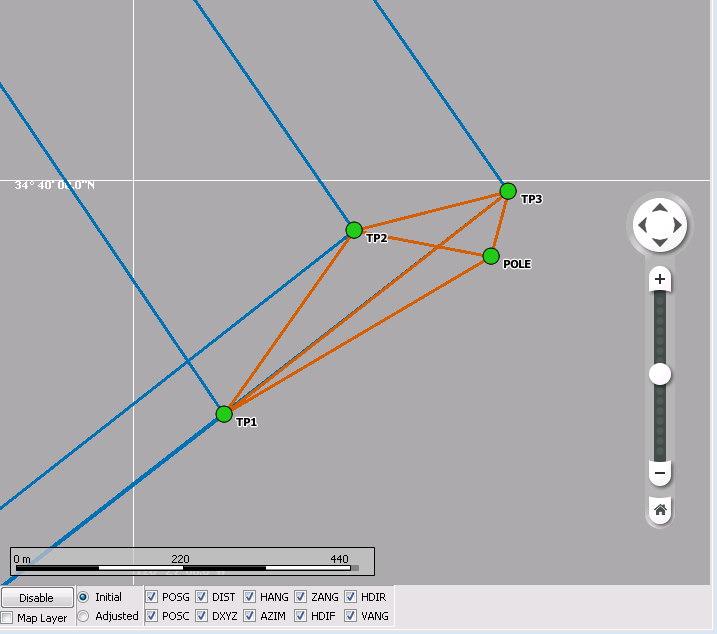
\includegraphics[width=0.7\textwidth]{example01/networkdesign}
\end{center}
\caption{Portion of Example 1 network.}
\label{fig:ex01networkdesign}
\end{figure}

We will build this example in several stages, and we will execute least squares adjustments at each stage.  This incremental approach is good practice, in that by solving several small problems we are better positioned to isolate and resolve errors than when we attempt one larger complex adjustment.

As we introduce each measurement type, we will show, via the Record Editor, how a user would manually create the measurements using the \textsf{salsa} interface.  However, we have also provided the measurement files in .lsa format so that the reader need not manually enter all these data.  Typically, we expect that users will have access to measurement files in .lsa format or in some other format that is easily converted to .lsa, such as GeoLab .iob files.

\subsection{Create New Project}
As a general rule, the authors recommend organizing a project's data within a common folder.  Although SALSA can read data files located outside the project folder, keeping all the project data together keeps the organization simple for the user and simplifies subsequent transfer or archival of the project.

We'll create a new project called \verb+example01+ in a folder by the same name on our Desktop.  Launch \textsf{salsa}, then use the menu action Project $\to$ New... and browse to the \verb+Desktop/example01+ folder (creating it if necessary), and specify the project file name \verb+example01.proj+.  (We could use any file extension we want, but \verb+.proj+ is a convenient convention for \textsf{salsa} project files.)

Upon creating a new project in this fashion, \textsf{salsa} will generate the new file \\\verb+example01.proj+, a nearly empty file containing only a single comment record that indicates the date and time of project creation.  \textsf{salsa} will also copy the default configuration file from the \textsf{salsa} installation directory into the project directory, giving it the name \verb+example01.cfg+.  The \textsf{salsa} interface will look like Figure \ref{fig:ex01newproj} at this point.

\begin{figure}[!htbp]
\begin{center}
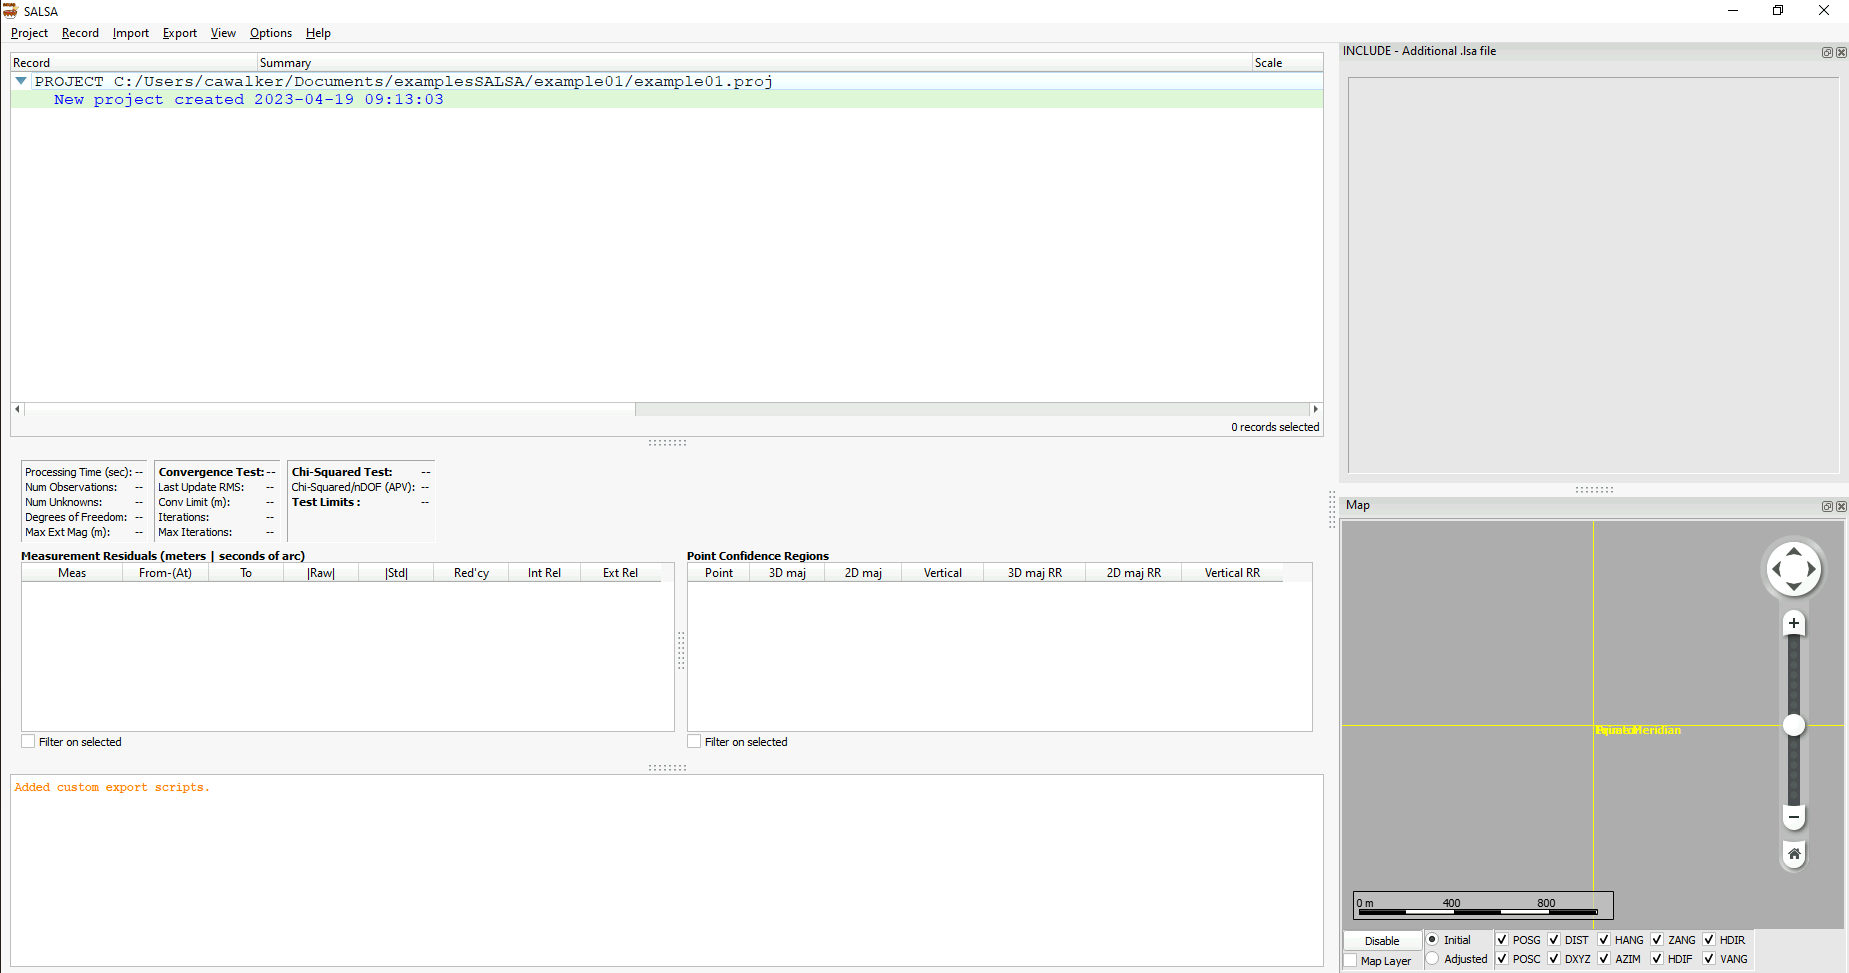
\includegraphics[width=0.99\textwidth]{example01/newproj}
\end{center}
\caption{The Salsa interface upon creating our new project.}
\label{fig:ex01newproj}
\end{figure}


\subsection{Introduce Control Points}

Our control network includes the sites listed in Table \ref{tab:ex1control}.

\begin{table}[htb]
\caption{Example 1 Control Network}
\label{tab:ex1control}
\begin{center}
\begin{tabular}{lrrr}
\hline
\textbf{Site} & \textbf{X Coordinate} & \textbf{Y Coordinate} & \textbf{Z Coordinate} \\
\hline
VNDP & -2678090.4859 m & -4525437.0277 m & 3597431.9403 m \\
P513 & -2669569.2656 m & -4504986.4064 m & 3629597.4450 m \\
\hline
\end{tabular}
\end{center}
\end{table}

We could at this point start keying in records representing our control sites, but in the interest of developing good habits, we will instead organize these position records in their own dedicated file which is to be included in our main project.  To do so, we need to insert an empty `include' record referencing the new file we wish to create.

Note that in \textsf{salsa}, when we insert a record, the new record will be inserted after the currently-selected record \emph{at the same hierarchy level} (i.e., in the same file as the selected record).  In the case of inserting a new project-level include, either the Project Include record or any record directly within the project level may be selected.

Therefore, select either the Project Include record or the comment record, then use the menu action Record $\to$ Insert $\to$ New Include to include our new file.  When prompted by the file explorer, provide a name such as \verb+control.lsa+.  Now the \textsf{salsa} Project Navigator shows \verb+control.lsa+ within our project, and if we click the little triangle next to this Include record, we see that this new included file is empty except for a single comment.

Now we'll insert our position records.  Since we want our new position records to be \emph{inside} the \verb+control.lsa+ file, we need to select a record within that file, i.e., the comment record.  Figure \ref{fig:ex01treewithnewinclude} shows the Project Navigator at this state, with the comment record selected.

\begin{figure}[!htbp]
\begin{center}

\includegraphics[width=0.8\textwidth]{example01/treewithnewinclude}
\end{center}
\caption{The Salsa Project Navigator after inserting a new Include record to contain position records for a control network.  Note the currently selected record (a comment record) is inside \texttt{control.lsa}; therefore a subsequent Record $\to$ Insert operation will yield a new record inside \texttt{control.lsa} as desired.}
\label{fig:ex01treewithnewinclude}
\end{figure}

Therefore, select the comment within \verb+control.lsa+ and proceed with menu action Record $\to$ Insert $\to$ POSC (Station Position Cartesian).  This will result in a new, selected, POSC record with its attributes available for editing in the Record Editor.  Now we can key in the first station name and coordinates as listed in Table \ref{tab:ex1control}.  Since these are control sites, set the position's Type to Fixed.

We could now proceed with menu action Record $\to$ Insert $\to$ POSC to create a record for site P513 as well.  However, entering all of the associated data (and all the measurements we'll get to momentarily) is very tedious, so the authors have provided input files that can be imported into this project.  Let's take advantage of those!

Example data are included in the SALSA installation directory; on Windows systems this will typically be \verb+C:\Program Files\SALSA\examples\+.  Copy the contents of the \verb+example01+ directory into the \verb+example01+ folder you already created on your Desktop. (Note: Please utilize the examples directory only for copying data as some user permissions may not allow writing to this directory.)

Now, in \textsf{salsa}, delete the \verb+control.lsa+ Include record by selecting the record and pressing the delete key or by menu action Record $\to$ Delete.  Replace the deleted record by inserting \verb+ctrl_sites.lsa+ (which we just copied into our project folder) via the menu option Import $\to$ Include from LSA\ldots (or F6); when prompted, select the file \verb+ctrl_sites.lsa+.

Figure \ref{fig:ex01withcontrol} shows the \textsf{salsa} interface after the two control sites have been introduced to the project.  (The Include record has been expanded and the first POSC record selected.)

\begin{figure}[!htbp]
\begin{center}
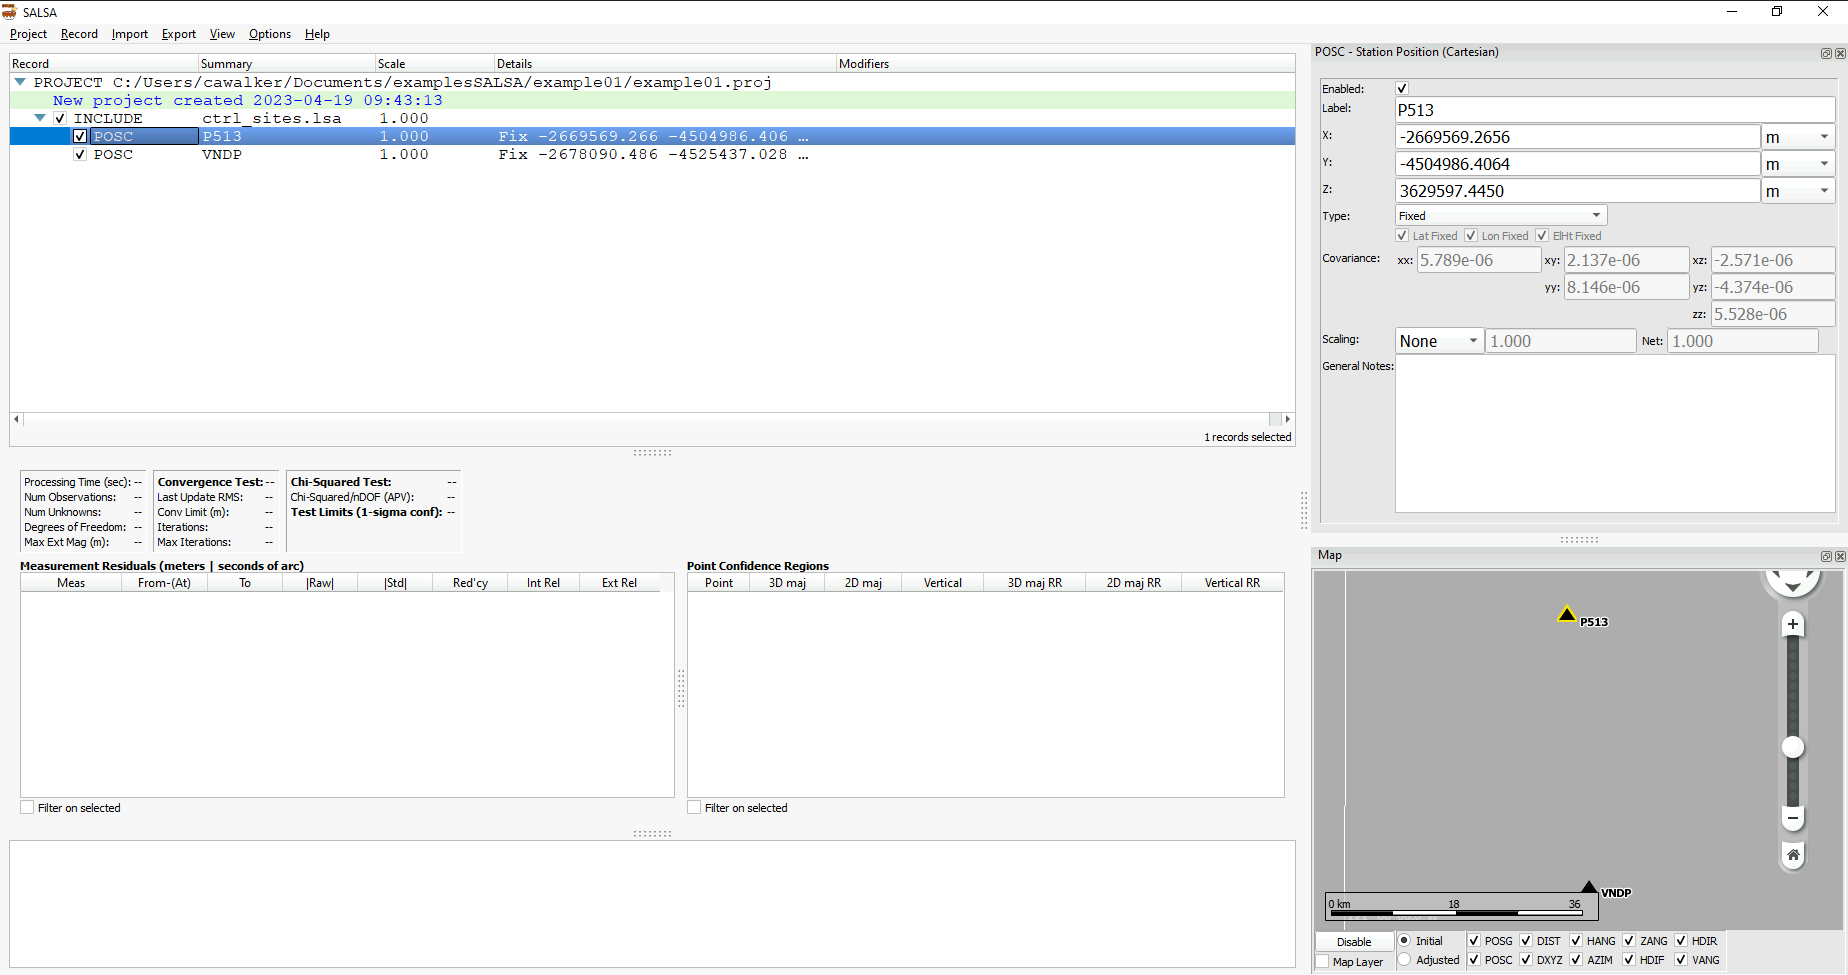
\includegraphics[width=0.99\textwidth]{example01/withcontrol}
\end{center}
\caption{The Salsa interface after inserting an Include record containing a small network of control sites.}
\label{fig:ex01withcontrol}
\end{figure}


\subsection{Execute GPS-only Adjustment}

Next, we will introduce GPS vector estimates to the project; these will be used to determine positions for the TPs.  These GPS vectors will share an uncertainty model (UNCR record).  Thus, we could proceed manually by creating a UNCR record and then keying in all the GPS vectors and covariance matrices, each time specifying that UNCR record.  Instead, we will take advantage of an lsa-formatted file already prepared in this way.

Ensure that the existing Include record in the measurement tree is selected, so that the next Include record we insert will be inserted at that same level of the hierarchy.  Then use the menu option Import $\to$ Include from LSA\ldots and when prompted, select the file \verb+gpsMeasurements.lsa+.

Expand the \verb+gpsMeasurements.lsa+ Include record and take a moment to review the contents.  We see the UNCR record and six GPS vectors (DXYZ) relating the TPs to control sites VNDP and P513.  The Details column of the Project Navigator shows the lengths of each vector.  Select the UNCR record and look at the attributes shown in the Record Editor.  It's been given a meaningful label `UNCR\_DXYZ\_STATIC' and contains two non-zero components, a to-station centering error and a from-station centering error. Both errors have a value of 1.0 mm.  These error terms will be combined with the uncertainty (covariance matrix) specified with any measurements referencing this UNCR record; each of the GPS vectors reference this UNCR so any uncertainties specified by their individual measurements will consider the aforementioned error terms.

Select one of the DXYZ records and review its attributes in the Record Editor.  We see the From and To sites specified, the X/Y/Z vector components, and the upper triangular covariance matrix components.  We see that the `UNCR\_DXYZ\_STATIC` uncertainty model has been specified.

Note that the Scaling for each measurement is set to None, for an effective value of 1.00. This is also a good time to point out the Scale column in the Project Navigator. Each Include record includes a scale term. By default, this is set to None (1.000), however the user may specify a VSCA label or numeric value and this value will be propagated to each of the child records associated with the Include. Later in this example we will use this field to manipulate the scaling of the uncertainty in our observations to achieve a properly balanced observation set.

Also note that our map looks pretty plain; we don't see the GPS vectors we just added, nor do we see the TPs.  This is because \textsf{salsa} doesn't yet know the location of the TPs\ldots

We can now proceed with a least squares adjustment of these GPS vectors.  If we were to select the menu action Project $\to$ Calculate Adjustment, initial coordinates for the TPs would be determined, and the least squares solution would commence.  But instead of jumping right to the network adjustment, let's take advantage of \textsf{salsa}'s menu action Project $\to$ Generate Initial Positions (do save when prompted).  This action actually initiates a solution (using \textsf{lsasolver} behind the scenes) but aborts immediately after determining the initial coordinates of any unknown points, such as our TPs.  This action can be useful to users in that it facilitates rendering of the measurement network in the map, and the user has an opportunity to `sanity check' the problem before commencing with a least squares solution.

After generating the initial positions, observe that they (the TPs) are now shown in the Project Navigator, under a new Include record near the top labeled `Auto-generated Initial Coordinates.'  Each of these `auto-generated' POSG records is depicted with a little gear image to remind the user they are automatically determined and were not part of the user's problem definition.  These will be overwritten each time the user calculates an adjustment.  These records are not editable (except for their station label), and they cannot be copy-pasted elsewhere into your project.  You may delete them, since they will just be auto-generated again the next time you calculate an adjustment.

Though doing so now is not advised unless this example has been previously executed successfully at least once, auto-generated POSG records may be permanently added to a project; do so by running Project $\to$ Calculate Adjustment, opening the final positions table via View $\to$ Final Positions, selecting an auto-generated point, then right clicking to access and select the Add to project as Float option.  Doing this will make the gear icon disappear and the POSG record become persistent, moving the POSG into a new Include record (and file on disk) \verb+initial_coordinates.lsa+.  Thereafter, the file will be used as input to the solver and will not be overwritten when calculating an adjustment.

Now that we have initial positions estimated for the TPs, the TPs show up in our map, as do the GPS vectors to the control points.  Note that auto-generated positions are depicted with `?' on their markers. (If the adjustment was already calculated in order to permanently add the auto-generated POSG records to the project, the Initial radio button below the map may need to be re-selected to display the initial auto-generated positions with their `?' symbols.)

Take a few moments to experiment with the map controls.  Panning and zooming can be done with mouse actions (click-and-drag, and scroll, respectively) or by using the navigation controls overlaid on the map.  (If you prefer, you can instead use the arrow keys on your keyboard to pan, and +/- to zoom.)  Note the little `home' button in those controls; it will redraw the map to include everything in our network.

Zoom into the cluster of TPs on the map.  Note that when you select an item in the map (by clicking on it), it also becomes selected in the Project Navigator.  Conversely, when you select a record in the Project Navigator, it becomes selected (highlighted) in the map.  This coupling of the interfaces is intended to help users visualize their measurement network and troubleshoot blunders or other errors.

Since our network appears to be sane, let's proceed with an adjustment.  First, we will disable reliability metrics. Reliability metrics are turned on by default but are not the focus of this example. They are the primary focus of \verb+example02+. To disable reliability metrics, first open the Configuration Menu by selecting the menu action Project $\to$ Configure\ldots and under the Solver Options box, select the \verb+no+ button next to Calculate External Reliability. Press \verb+OK+ at the bottom of the Configuration Menu to accept the changes and close the window. Use the menu action Project $\to$ Calculate Adjustment (or F5).  Save when prompted.

Wow!  Lots of things just happened in the \textsf{salsa} interface!  Reference Figure \ref{fig:ex01gpsadjust}.  Just below the Project Navigator we see some summary information (processing time, degrees of freedom, etc.) and two important tests: the convergence test, and the Chi-squared test.  The convergence test shows that convergence was achieved, in 2 iterations, and the test indicates PASS.  However, the Chi-squared test does not pass with the default confidence level of 1-sigma. The significance of this result will be discussed momentarily, for now let's proceed to investigate other components of the \textsf{salsa} interface.

\begin{figure}[!htbp]
\begin{center}
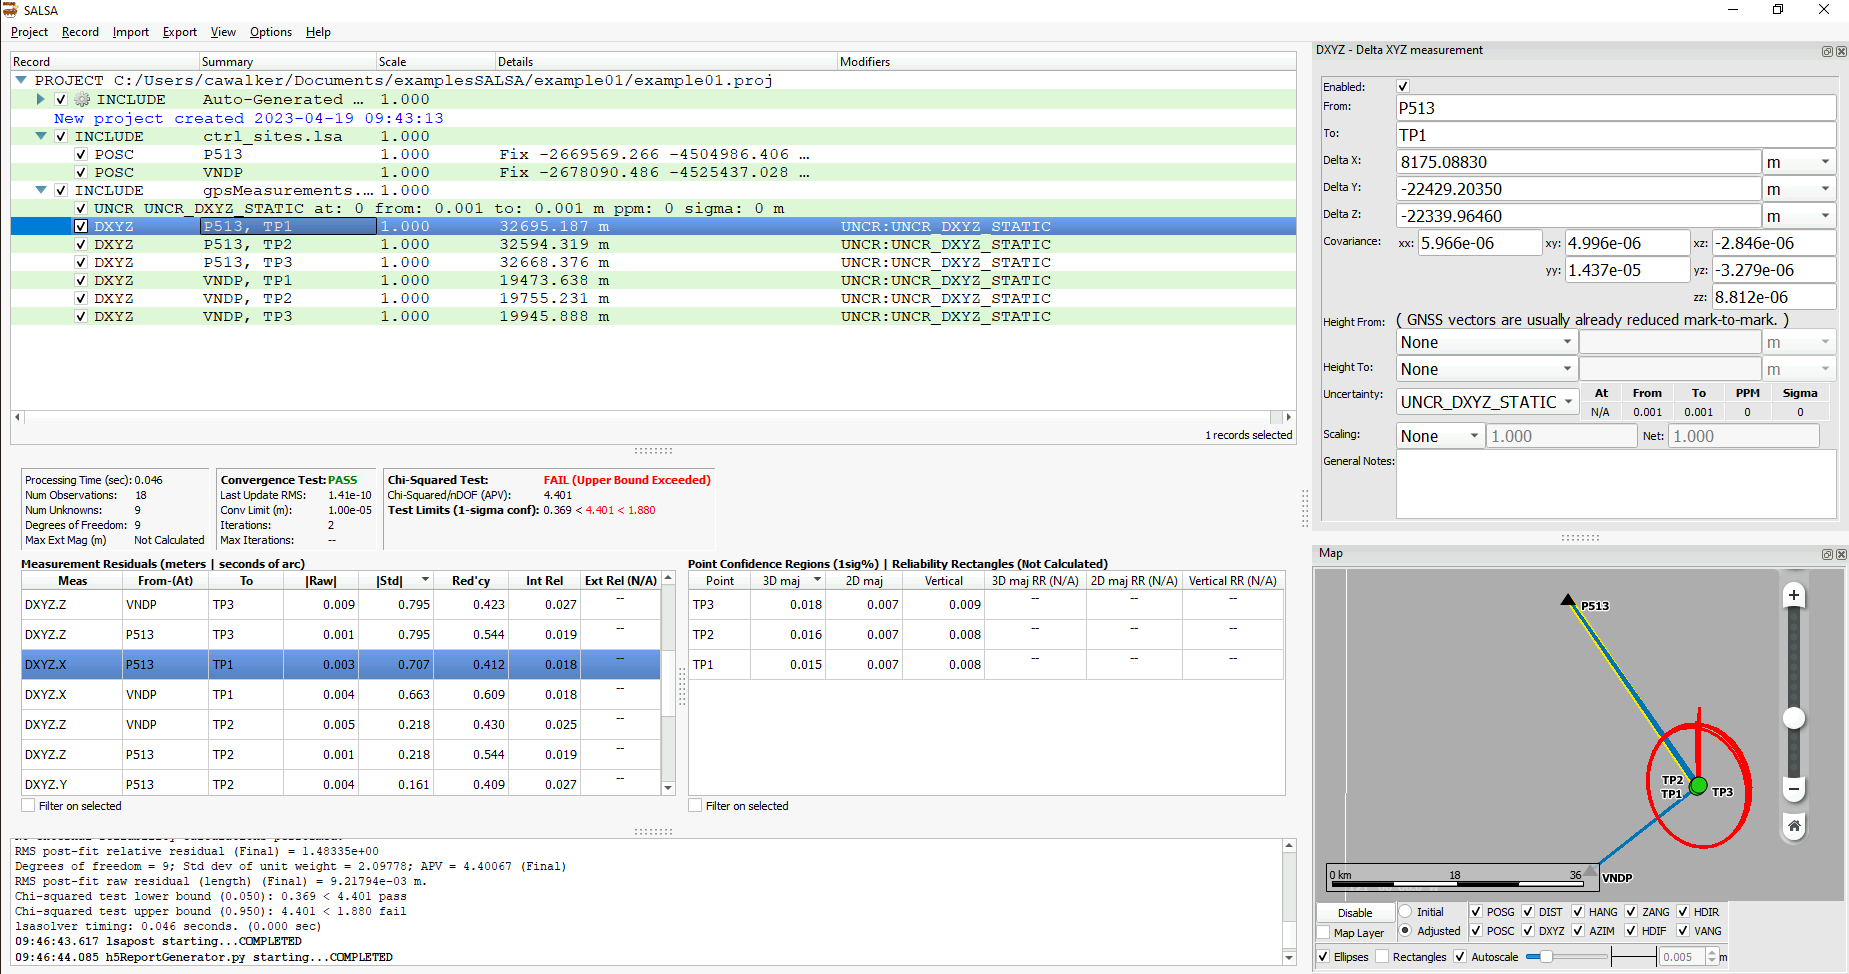
\includegraphics[width=0.95\textwidth]{example01/gpsadjust}
\end{center}
\caption{The Salsa interface after running the GPS-only adjustment.}
\label{fig:ex01gpsadjust}
\end{figure}

Below these convergence and Chi-squared test summaries we see a Measurement Residuals table, which by default lists each measurement in descending order of standard residual magnitude.  Note that DXYZ vectors are listed in this table by individual components (X, Y, Z). If any measurement standard residual exceeds the statistical test threshold as defined in appendix \ref{appendices:RedStdResComp}, the standard residual value is rendered in red text; no measurements in this example exceed the threshold. 

Now is a good time to again mention that reliability metrics are not calculated in this example. Because of this, a few of of the features in the \textsf{salsa} interface are disabled. First, the ``Max Ext Mag (m):'' heading is disabled. Next, the two rightmost columns of the Measurement Residuals table should be ignored. Lastly, the three rightmost columns in the Point Confidence Regions table as well as the checkbox labeled ``Rectangles'' in the mapping window should also be ignored. See \verb+example02+ for in-depth coverage of reliability metrics and their uses.

To the right of the Measurement Residuals table we see the Point Confidence Regions table.  This table lists all points in the network in descending order of their 3-D confidence region major axis length (the user can choose to sort by other columns).  Thus, points with the largest uncertainty are listed first.

In the status window at the bottom of the interface we see some output from the CLI applications that prepared the data (\textsf{lsapreprocessor}), executed the adjustment (\textsf{lsasolver}) and extracted results (\textsf{lsapost}).  Since this adjustment executed appropriately, there isn't too much of interest in here, but know that this output exists and is a good place to look for issues if the adjustment is not successful.

Finally, we note that the map has changed.  The map now shows the least squares problem output, not the input (observe the Initial and Adjusted radio buttons below the map which allow the user to switch between the two states.)  Our TPs are now rendered with error ellipses depicting their 2-D confidence regions.  The scale of the ellipses is shown below the map and can be adjusted by manipulating the slider.

So how did the adjustment go? The solution converged, no measurements were flagged as blunders and our point confidence regions are all sub-cm. However, given the high APV value of 4.401 raised a failure alert for the Chi-squared test, this should not be deemed a success. Generally, when the Chi-squared test fails this should be taken to mean that the data are discrepant with the model parameters. This can be attributed to blunders in the data or having overly optimistic sigmas that are small in value. Given that no blunders were raised in the measurement residuals table, the latter explanation seems a likely candidate.

Let's account for this by utilizing a variance scaling (VSCA) modifier. In the project navigator, select the UNCR record and proceed to click on Record $\to$ Insert $\to$ VSCA. Edit the label and Scale Factor values of the new VSCA record to GPS and 2.000 respectively. Multi-select all of the DXYZ records by clicking on the first DXYZ record, then press Shift + Left click on the last DXYZ record. Go to the Scaling dropdown box in the Record Editor and select GPS from the dropdown menu. Take a moment to observe that the Scale value for each of the DXYZ records is now 2.000.

Calculating a new adjustment will drop the APV to a more reasonable value of 2.200. Unfortunately, this still does not pass the Chi-squared test. At this point, we could go back to our VSCA record and increase its value further; instead, let's try an alternate method of boosting the variance scaling of the DXYZ records. Find and click on the \\\verb+gpsMeasurements.lsa+ Include record. In the Record Editor, click on the Scaling dropdown box and select Value, then set the number next to the dropdown box to be equal to 2.000. Upon hitting the Enter key, the user will observe that the scale values of our DXYZ records are now equal to 4.000. Setting a scale value (either by entering the value directly or through a VSCA record) on the parent Include record will propagate to each of the child records. However, since each child DXYZ record also utilizes the GPS VSCA modifier, the scale for those DXYZ records is the product of their VSCA modifier and the scale of the parent Include record. Calculating a new adjustment now yields a Chi-squared value of 1.100, which passes the test.

\subsection{Add TP Conventional Network}
We will now add the conventional observations between the TPs.  These observations include direction sets, zenith angles, and distances.  Again, keying these data manually would be very tedious, so please take advantage of the prepared files provided with SALSA. In the Project Navigator, select our last Include record \\\verb+gpsMeasurements.lsa+ (so that the next include will be inserted at this same level in the hierarchy).  Then use menu action Import $\to$ Include from LSA\ldots  and when prompted, select the file \verb+conventional.lsa+.  Figure \ref{fig:ex01treewithtp} shows the Project Navigator once that file is included and expanded.

\begin{figure}[!htbp]
\begin{center}
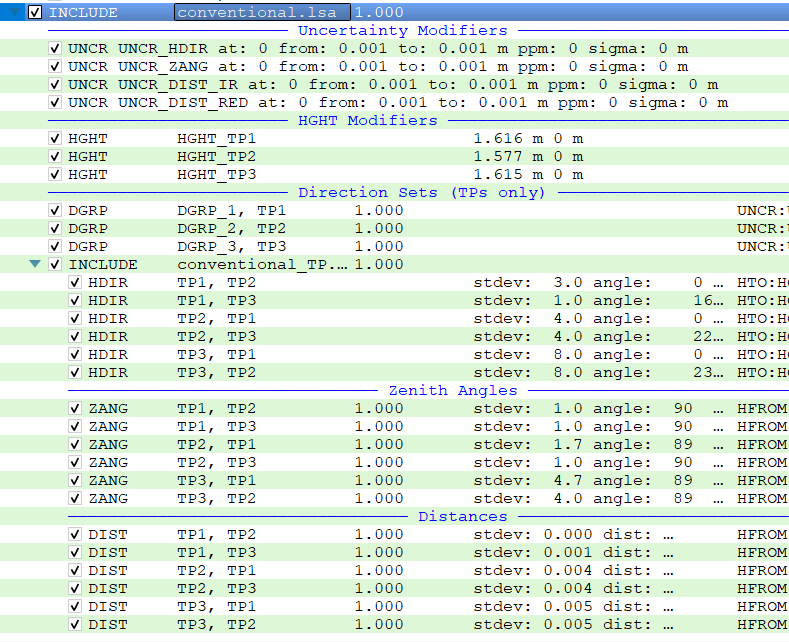
\includegraphics[width=0.7\textwidth]{example01/treewithtp}
\end{center}
\caption{Portion of the Salsa Project Navigator after adding conventional observations to the temporary points.}
\label{fig:ex01treewithtp}
\end{figure}

Take a few minutes to review the records we just inserted.  Select the different record types and review their attributes in the Record Editor.  Observe the organization of these records; instrument heights and uncertainty models are specified near the top, then the observations are specified by type within their own included file \verb+conventional_TP.lsa+: direction sets, zenith angles, and distances.  This is just one example of a project's organization; some users may prefer to group observations by setup instead.  SALSA is not order-dependent, giving the user flexibility to organize their project however they choose.  For example, the instrument heights could be specified \emph{after} the observations, and the solution will not be impacted.

Let's look specifically at instrument heights.  Select the first HGHT record, with label HGHT\_TP1.  The Record Editor shows just five attributes: Enabled, Label, Height, Sigma, and the General Notes field.  This record is enabled, and we could disable it by unchecking it in the Project Navigator or the Record Editor.  It has the label HGHT\_TP1 which is obviously a reference to the station name TP1.  Note, however, that this label can be any text that the user finds helpful that can uniquely identify this height and sigma value.  For example, if TP1 was set up and observed twice, once by Jack, and once by Sue, we will have two different instrument heights and sigmas for TP1, and we would create two HGHT records, perhaps one with label HGHT\_TP1-Jack and one with HGHT\_TP1-Sue (or morning and afternoon - whatever works!).  Further description can be kept in the General Notes field for later reference.

Now that we see that a height record is just an arbitrary label and a value, skip down to the first ZANG (zenith angle) observation, and let's see how these height records are referenced.  Figure \ref{fig:ex01zangrecord} shows the Record Editor with the first ZANG record selected.  Observe that this zenith angle is observed at station TP1 and is observing the zenith angle to TP2.  The Record Editor shows ``Height From:'' and there is a dropdown list of choices.  The currently-selected height record is the one we looked at moments ago, with label HGHT\_TP1, and we see that the value is shown next to it, 1.6160 meters.  Look at the other options.  We see the other height records available, and we see the choice ``Value.''  If we choose Value, the 1.6160 entry becomes editable, and we can type in a numeric value applicable to this individual ZANG observation.


\begin{figure}[!htbp]
\begin{center}
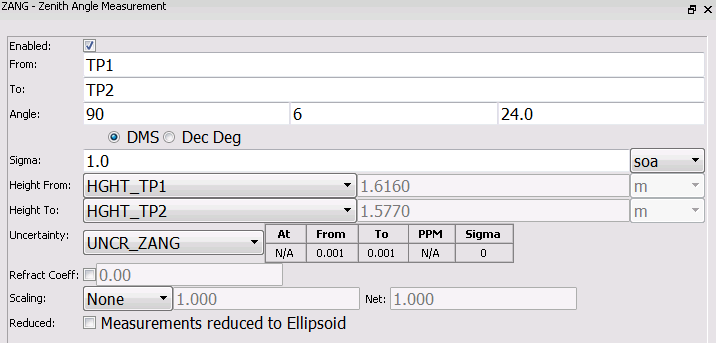
\includegraphics[width=0.7\textwidth]{example01/zangrecord}
\end{center}
\caption{Record Editor showing the attributes of a ZANG (zenith angle) record.}
\label{fig:ex01zangrecord}
\end{figure}


The point we hope the reader takes from this close look at these height and ZANG records is this:  \textsf{salsa} provides the flexibility to key in these values directly, but a smarter scheme is to define these attributes (height of instrument, uncertainty model) with descriptive labels, and then specify those `modifiers' by name in the individual measurement records.  This way, the user only needs to make an edit in one place (the referenced HGHT or UNCR record) to update all the measurements referencing that modifier. At this point, proceed to calculate an adjustment. The APV still passes for our updated network with an APV value of 1.042.


\subsection{Add Conventional Observations to Target}

Finally, let's add the conventional observations to the inaccessible target, which is the subject of this survey after all.  These observations are provided in the file \verb+conventional_tgtPole.lsa+, so select the Include record in our project tree \\\verb+conventional_TP.lsa+ (located as a child record in the \verb+conventional.lsa+ Include record), then  use menu action Import $\to$ Include from LSA\ldots and when prompted, select the file \verb+conventional_tgtPole.lsa+. Expand it in the Project Navigator and observe that there are three groups of observations, this time organized by measurement type. The observation sets include direction sets, zenith angles, and distances to a new-to-this-project site named POLE.  Note that these observations reference the same height (HGHT) records and uncertainty models (UNCR) that we defined inside the TP-only file.

Proceed with an adjustment (F5). Similar to the GPS only adjustment we can observe that the convergence test passes with sub cm confidence intervals. However, the Chi-squared test now fails with a value of 6.595 and there are now two ZANG records highlighted red in the Measurement Residuals table. Our first diagnosing tool that should be utilized for probing discrepant data is the measurement residuals table. Sort the rows by the \textbar Std\textbar\ column. At the top two entries the outlying ZANG data records can be observed. Upon closer inspection the user may notice that two of the top three entries are ZANG measurements with POLE serving as the To point.

With the prevalence of ZANG records at the top of our Measurement Residuals table, it seems prudent to investigate these measurement types further. From the menu select Record $\to$ Find/Filter (or Ctrl+F). The Filter row will contain a dropdown box with a default value of 'All Records'. Click on the box and scroll until you find an option labeled ZANG. Once found, click on the option to leave only ZANG records and their associated parent Include records. Scrolling through the individual sigmas, it can be observed that many have reported sigmas as low as 1 arc second. Exit out of the Filtered view by clicking the x in the upper right hand corner of the Find/Filter box. Find the UNCR records under the \verb+conventional.lsa+ Include record and select the `UNCR\_ZANG` uncertainty modifier. Navigate to the Sigma row in the Record Editor and modify the sigma value to be 3.0 soa.

Calculating an adjustment will lower the APV to a more reasonable value of 3.030, but the Chi-squared test still fails. At this point, we will introduce another useful diagnostic tool, the Histogram Dialog box. Select View $\to$ Histogram to observe the Histogram Dialog box present in Figure \ref{fig:ex01Histogram}. The histogram utility displays all of the measurement residuals in one plot while allowing the user to switch on or off measurement types or files from the residuals view as well. On the tail ends of the histogram, we can observe that two ZANG measurements still appear to be outliers. Clicking on these two ZANG measurements on the two tail ends reveal that both of the measurements have POLE serving as the To station...

\begin{figure}[!htbp]
\begin{center}
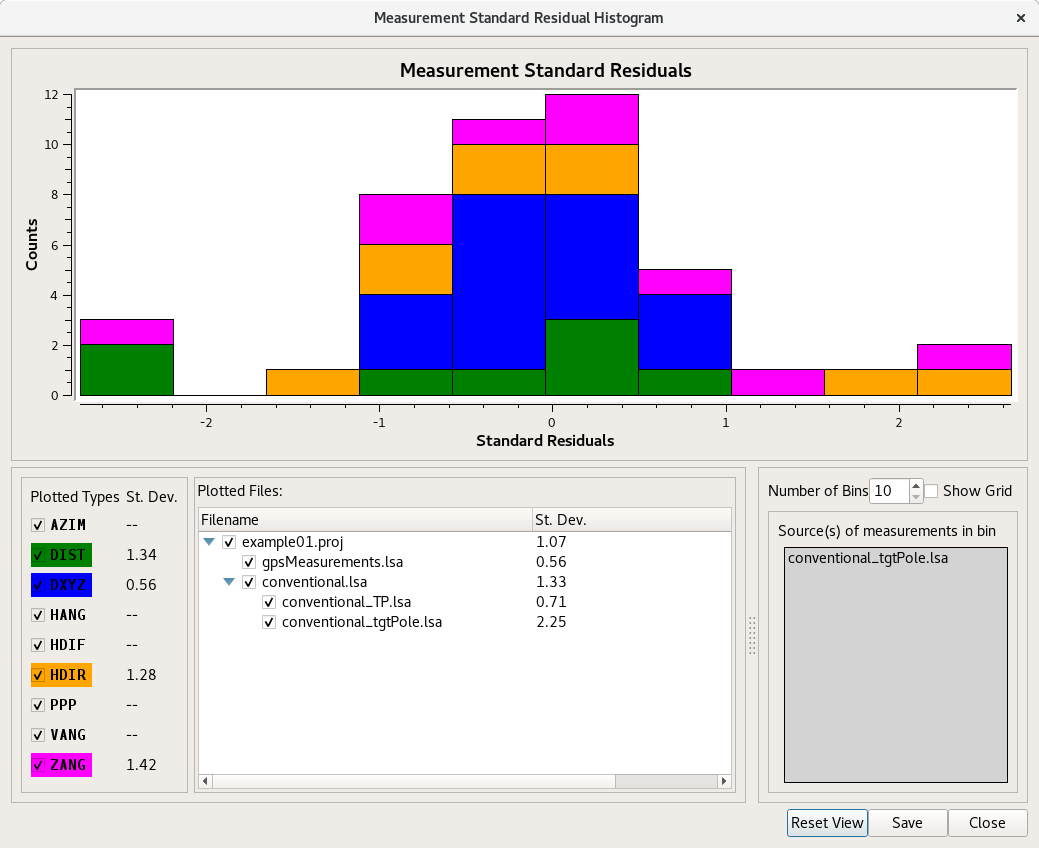
\includegraphics[width=0.7\textwidth]{example01/histogram}
\end{center}
\caption{Measurement histogram with APV value of 3.015}
\label{fig:ex01Histogram}
\end{figure}

Go ahead and close out of the histogram. Navigate to the Zenith Angles section of the \verb+conventional_tgtPole.lsa+ Include record and create a new UNCR record by selecting the menu option Record $\to$ Insert $\to$ UNCR. Assign its label a value of `UNCR\_ZANG\_POLE`; its From Centering Error a value of 1 mm; its To centering error a value of 1 cm and its Sigma a value of 10.0 soa. Multi select all of the ZANG measurements under \verb+conventional_tgtPole.lsa+ and select `UCNR\_ZANG\_POLE` from the Uncertainty dropdown box. Calculate an adjustment to observe a new APV value of 2.300. Though the Chi-squared test has not passed yet, the POLE ZANG measurements are no longer at the top of our measurement residuals table. Opening up the Histogram again, the user can also verify that the ZANG measurements are no longer present at the two end tails. The POLE DIST measurements now appear at the top of the measurement residuals table.

Upon selecting either of the DIST measurements in the \verb+conventional_tgtPole.lsa+ Include record, it can be seen that both measurements contain a reference to the `UNCR\_DIST\_RED` uncertainty modifier. Navigate to the Uncertainty Modifiers section under the \verb+conventional.lsa+ Include record and select the `UNCR\_DIST\_RED` uncertainty modifier. To verify that this modifier is only associated with the POLE DIST measurements, right click `UNCR\_DIST\_RED` and select Select Referencing from the menu. The desired measurements (and only the desired measurements) are highlighted appropriately. Select the `UNCR\_DIST\_RED` uncertainty modifier and modify its sigma value to be 3 cm. Recalculating an adjustment yields a passing value of 1.082.

\subsection{Review and Summary}

Zoom in on the map to the small network of TPs and our target POLE. Note the relative sizes of the error ellipses; it is reasonable that the uncertainty in POLE is larger than for our TPs which benefited from GPS vectors. Our Point Confidence Regions table shows that the uncertainty in POLE's final position estimate is at the cm level, at 1-sigma confidence level. The current choice of confidence level is displayed at the top of the Point Confidence table and can be changed in the Configuration Menu. Figure \ref{fig:ex01final} shows the map view at this stage.   

\begin{figure}[!htbp]
\begin{center}
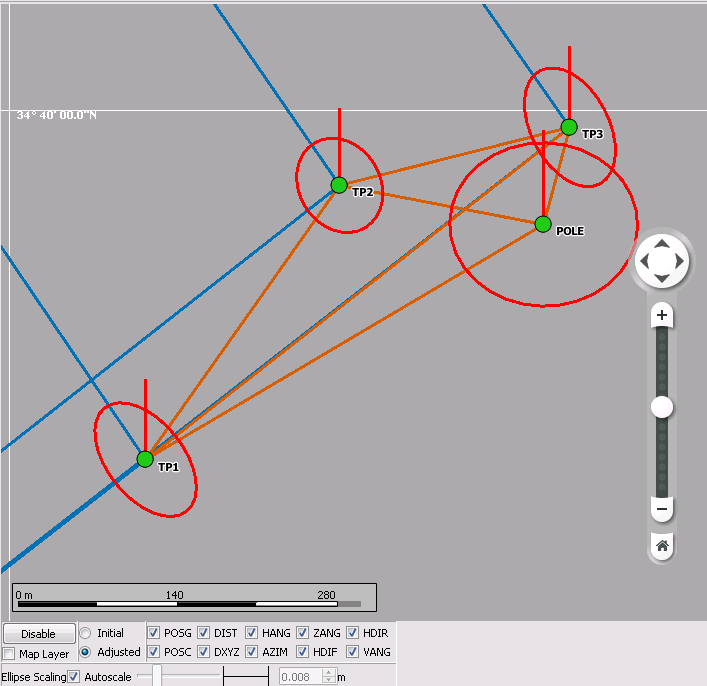
\includegraphics[width=0.7\textwidth]{example01/final}
\end{center}
\caption{Map showing TP and Target adjusted coordinates and confidence ellipses.}
\label{fig:ex01final}
\end{figure}

Before leaving this example, let's take note of three output files that have been generated each time we have run an adjustment.  All should exist in the \verb+example01+ folder containing our project.

The first is the log file produced by \textsf{lsasolver}, named \verb+example01.out+.  Since this example problem ran well for us, and we were able to troubleshoot a few discrepant measurements using the \textsf{salsa} GUI, we really didn't find ourselves needing to dig into the log file for this example.  However, the reader is encouraged to scan through this log file, relying on the explanation in Section \ref{sec:howtoreadoutfile} as a guide.

The second is \verb+example01.pts+ which is a simple text file containing all the points involved in this adjustment.  This file can be opened via the menu action View $\to$ Final Positions and is intended to give the user a quick look at the output in tabular format.

The third is a comma-separated values file named \verb+example01.csv+.  This file also contains the adjusted coordinates but in a format easily opened using your favorite spreadsheet program.


\section{Example 2: Redundancy and Reliability}

Example 1 illustrates some of the indicators SALSA uses to help the user recognize that a problem exists (e.g., the failing Chi-squared test and elevated APV), and how these indicators can help the user isolate the problem (e.g., by flagging measurements with high residuals). This example illustrates additional important indicators of the solution quality: the \emph{redundancy} and \emph{reliability} metrics. Redundancy is critically important in a geodetic least squares problem, and thus the user should ensure the network contains sufficient redundancy in order to have confidence in the final result. The confidence is mainly expressed through reliability metrics, which will be the focus of this example. 

In essence, reliability metrics inform the user of the network's susceptibility to blunders. This is done through three metrics: local reliability (also known as redundancy), internal reliability, and external reliability. The first half of this example will inform the user of the causes and indicators in SALSA of low redundancy. The second half will focus on the external reliability metric to show the impact of low redundancy on affected points in the network.

Please reference Appendix \ref{chap:solverout} titled ``Understanding the Solver Output'' for a brief explanation of redundancy and reliability metrics and references therein for further reading. Reference Appendix \ref{appendices:RedStdResComp}, ``Reliability and Standard Residuals,'' for a comprehensive treatment of these Reliability metrics.

To execute this example, copy the \verb+example02+ folder from the SALSA installation directory (i.e., \verb+C:\Program Files\SALSA\examples\example02+) onto your desktop or other convenient location.  Start \textsf{salsa} and open the project file \verb+redundancy.proj+ (Project $\to$ Open LSA\ldots).  For the first part of this example, make sure \textsf{salsa} is \emph{not} configured to compute external reliability:
\begin{itemize}
  \item Project $\to$ Configure\ldots
  \begin{itemize}
    \item Calculate External Reliability = No
    %\item External Reliability Warning (m) = 0.5
    %\item External Reliability Error (m) = 1.0
  \end{itemize}
\end{itemize}

Then run the adjustment (F5). Figure \ref{fig:ex02firstrun} shows the \textsf{salsa} interface after the adjustment, and Figure \ref{fig:ex02initialmap} provides a zoomed-in view of the network design within the map view. 

\begin{figure}[!htbp]
\begin{center}
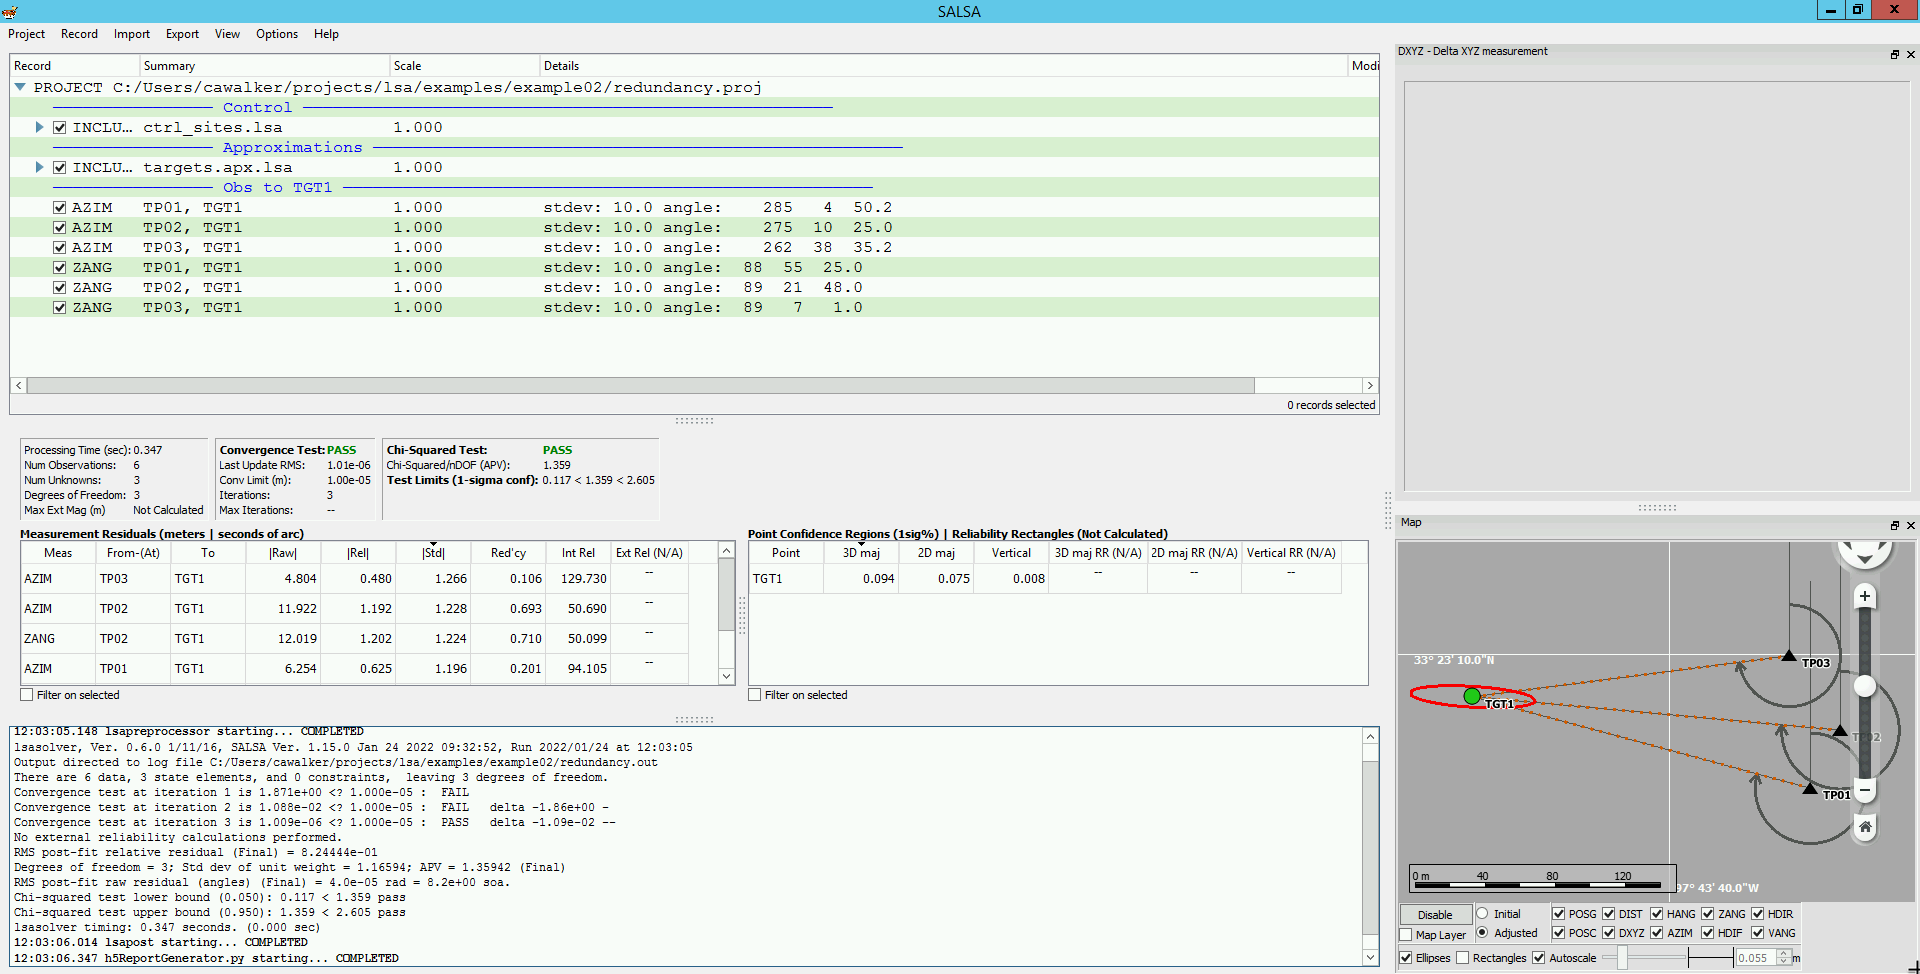
\includegraphics[width=0.99\textwidth]{example02/after_first_solution}
\end{center}
\caption{\textsf{salsa} interface for redundancy project, after adjustment.}
\label{fig:ex02firstrun}
\end{figure}

\begin{figure}[!htbp]
	\begin{center}
		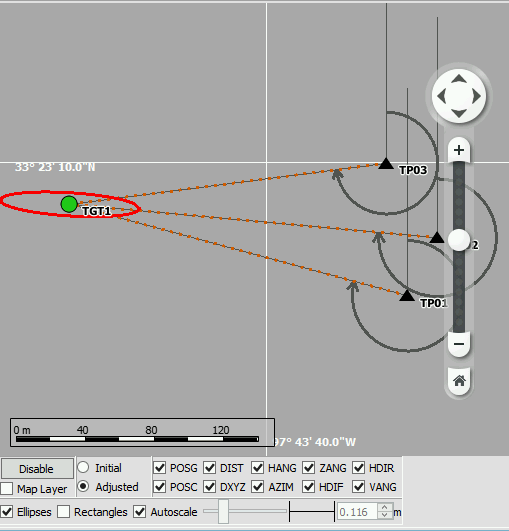
\includegraphics[width=0.7\textwidth]{example02/initial_map}
	\end{center}
	\caption{The redundancy project survey network.}
	\label{fig:ex02initialmap}
\end{figure}

There are three fixed points to the east, and a single estimated target to the west. The target is estimated using the classic ``three-point intersection'' methodology: azimuths from each of the fixed points intersect at the target to determine horizontal position, and zenith angles from the fixed points determine the height component. Direction sets or horizontal angles could have used instead of azimuths, but azimuths are easier to show in this example.

This solution looks fine: The adjustment converged, the Chi-squared test passed, and no standard residuals are flagged as likely blunders.

What happens if the three-point intersection is reduced to a two-point intersection? To find out, select and disable the AZIM measurement record from TP03 to TGT1 and re-run the adjustment (F5). Note the solver still achieves convergence, the Chi-squared test passes with an APV near 1.0, and there are no high residuals. However, the two remaining azimuths to TGT1 show redundancy values very close to zero (0.001). In addition, the Int Rel column for these two measurements show values of approximately 1257 and 1413 SOA respectively. This means that any error in the measurement smaller than 1257 or 1413 SOA will be undetectable. Why this is a cause for concern will be shown later through external reliability. Save the output files \verb+.out+, \verb+.csv+, or \verb+.pts+ for reference later in this example.

Even though the solver successfully converges on a solution and the Chi-squared test passes, the redundancy metric indicates a major problem in the survey. Lacking redundancy means that any error in the measurements goes directly into the solution \emph{without any obvious indication to the user!}. 

To demonstrate this problem, select the AZIM record from TP02 to TGT1 and change the minutes value of the angle from 10' to 19' (simulating a user blunder). Then run the adjustment. Figure \ref{fig:ex02witherror} shows the state of the \textsf{salsa} interface at this point.

\begin{figure}[!htbp]
\begin{center}
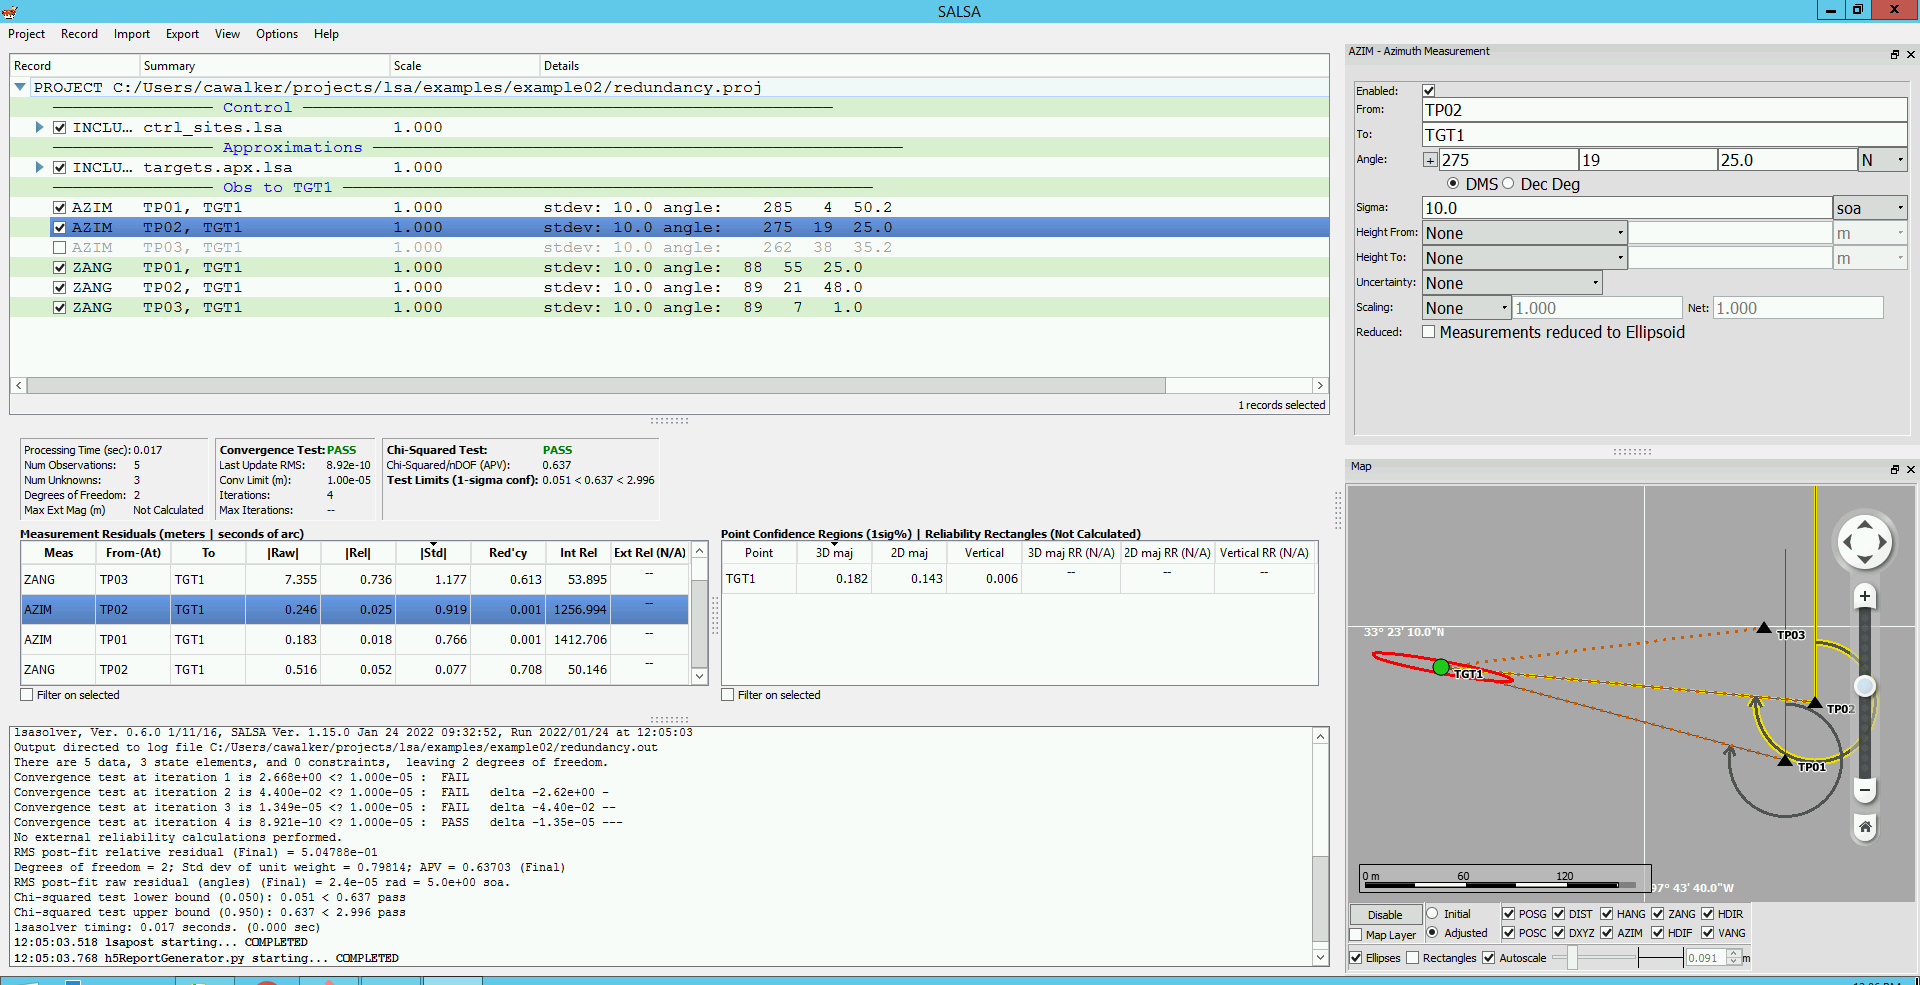
\includegraphics[width=0.99\textwidth]{example02/blunder_introduction}
\end{center}
\caption{Introducing a 9' blunder in the AZIM TP02 to TGT1 record (19' vs 10').}
\label{fig:ex02witherror}
\end{figure}

If the low redundancy metric is ignored, the solution appears satisfactory: it converges with no high residuals and a passing Chi-squared test. However, the final adjusted position of TGT1 is now over three meters shifted to the west due to this blunder. The shift in solution is observable by comparing the XYZ Final Adjusted Position for TGT1 in the \verb+.out+ output file from before and after the blunder error is introduced.  Take note: ignoring low redundancy in the network leaves you susceptible to measurement blunders with no obvious indication that an error has occurred.

Leaving the blunder error in place and re-activating the third azimuth record (from TP03 to TGT1), re-run the adjustment. Now the Chi-squared test blows up with an APV value of 718, a clear indication something is wrong. The Chi-squared test indicates whether the post-fit residuals (i.e. the difference between the observed and expected measurements) are aligned with the prescribed uncertainties of the measurements, so having 9 arc-minutes of error in one of the post-fit residuals relative to the expected 10 arc-seconds uncertainty produces a very high APV. However, as this example illustrates, errors in measurements that lack adequate redundancy do not yield high residuals and thus do not inflate the APV or cause the Chi-squared test to indicate a problem.  The user must understand that some redundancy is required for every measurement in the network in order to have full confidence in the final solution.

How much redundancy is required to achieve confidence in the solution?  This can be a difficult question to answer.  First of all, there is no single ideal minimum threshold that is appropriate for all geodetic survey problems.  Second of all, how can the surveyor know how poor redundancy in a given measurement actually affects their confidence in the final adjusted coordinates?  Fortunately, SALSA includes reliability metrics which may help answer these questions by mapping and quantifying the impact of low measurement redundancy into terms the user understands: final adjusted coordinates. Reliability metrics provide an intuitive and visual descriptor, called a ``reliability rectangle,'' which shows a zone wherein the solution cannot be verified based on elevated standard residuals alone. If the size of the rectangle exceeds the user's tolerance for unchecked errors, then the user knows they must add additional measurements to the network.  A deep dive into the mathematical basis behind reliability metrics can be found in appendix \ref{appendices:RedStdResComp}, ``Reliability and Standard Residuals.''

Reliability metrics are normally enabled by default. However, reliability calculations were turned off by at the beginning of this example and will have to be manually re-enabled.  Go ahead and enable reliability calculations, and adjust the warning and error thresholds as follows:
\begin{itemize}
  \item Project $\to$ Configure\ldots
  \begin{itemize}
    \item Calculate External Reliability = Yes
    \item External Reliability Warning (m) = 0.5
    \item External Reliability Error (m) = 1.0
  \end{itemize}
\end{itemize}

In the Tree View, locate and disable the third azimuth record (TP03 to TGT1) again. Recalculate the adjustment.

\begin{figure}[!htbp]
\begin{center}
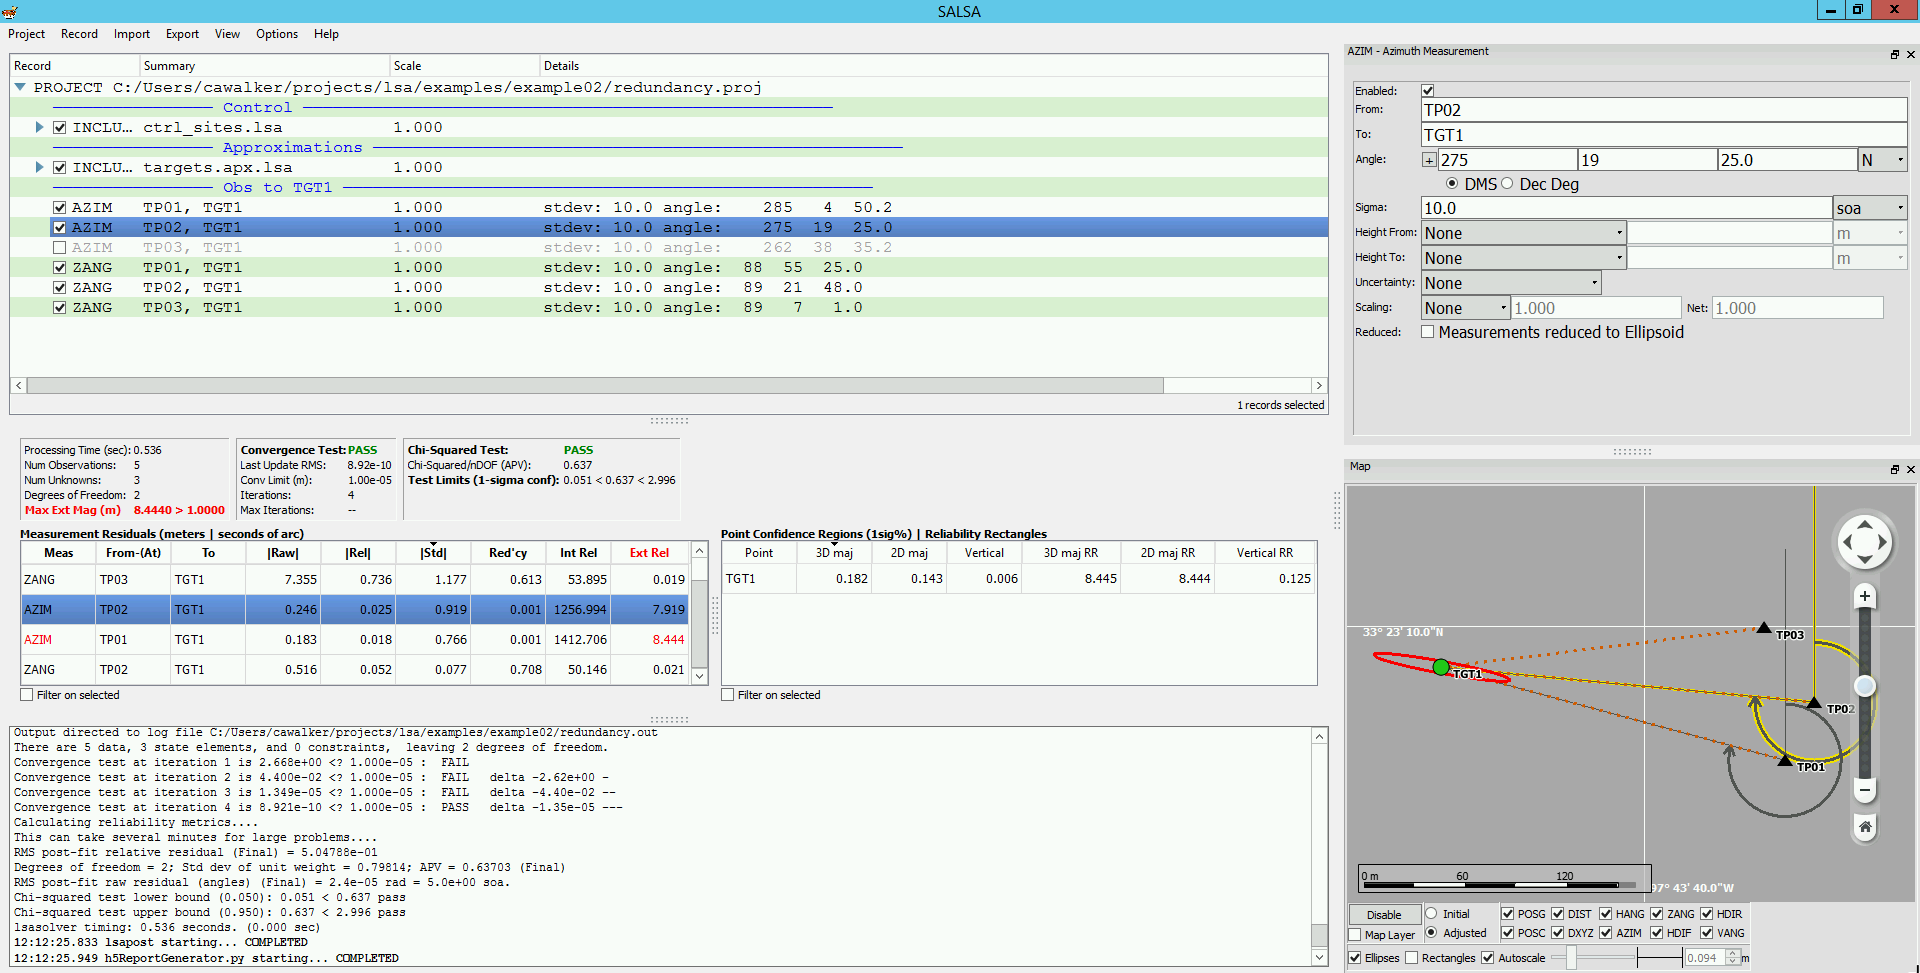
\includegraphics[width=0.99\textwidth]{example02/with_reliability}
\end{center}
\caption{Output with reliability metrics included}
\label{fig:ex02withReliability}
\end{figure}

Recall that earlier, even with the 9' blunder, there was nothing obvious in the \textsf{salsa} output to draw our attention to any problem.  Now, looking at Figure \ref{fig:ex02withReliability}, immediate changes are noticeable. First, the Ext Rel (external reliability) column header in the Measurement residuals table is highlighted red and the column has been filled with meaningful values instead of dashes, unlike before. Within the table, the user can see the two AZIM measurements are flagged with values that are 7.919 and 8.444 meters respectively. Above the Measurement Residuals table, the text ``Max Ext Mag (m): 8.4440 $>$ 1.0000'' is also highlighted red. This value represents the maximum external reliability value for all measurements and indicates whether that value constitutes an error (red) or a warning (orange) based on the user-configurable thresholds we edited moments ago.  In addition, the Point Confidence table now displays three additional numbers beyond the ellipse values: 3D maj RR, 2D maj RR, and Vertical RR. These values represent the 3D and 2D major axes of the reliability rectangle as well as the vertical component of the reliability rectangle.

What does all of this mean? Because the maximum external reliability magnitude calculated is 8.444 meters, any error in a measurement (i.e., blunder) that affects the estimated position by less than 8.444 meters is undetectable. In other words, the solution exists in a zone (reliability rectangle) indicating how much the solution could change due to a blunder \emph{without registering elevated measurement residuals.}

To highlight the scale of the reliability rectangle for this example, Figure \ref{fig:ex02rectangle} shows the reliability rectangle enabled in the mapping window. Note the reliability rectangle is enabled by selecting the corresponding checkbox in the mapping window. The rectangle is cyan by default; however, the user has the ability to change the color, line style, and line width in the menu Preferences $\to$ Map Preferences...

\begin{figure}[!htbp]
\begin{center}
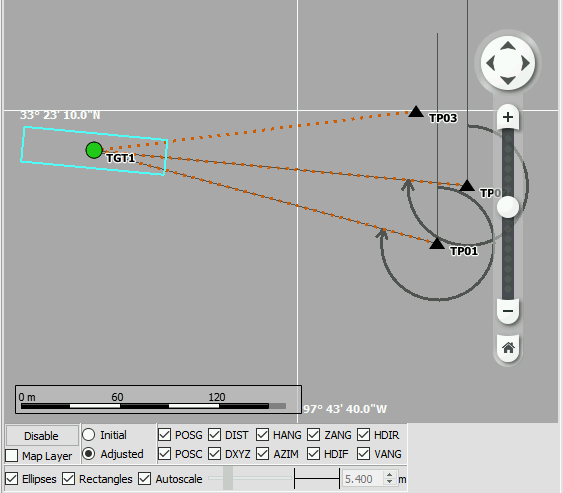
\includegraphics[width=0.99\textwidth]{example02/rectangle}
\end{center}
\caption{Reliability rectangle with one AZIM record disabled (2-point intersection).  Note the scale of the map shows the rectangle is several meters in size.}
\label{fig:ex02rectangle}
\end{figure}

\newpage

At first inspection, it may appear that the point confidence regions (ellipses) were disabled, but in fact, the TGT1 ellipse is so small in comparison to the reliability rectangle that it is invisible. While the survey result exhibits adequate precision (i.e., sub-meter error ellipse), the lack of redundancy yields a reliability rectangle that highlights the susceptibility of the survey result to a single undetectable error.

Now, re-enable the third AZIM measurement and recalculate the adjustment. The reliability results change drastically. The ``Max Ext Mag(m):'' value has dropped to 0.3227 meters; the survey design is now capable of detecting a multi-meter error as has been introduced in our AZIM record from TP02 to TGT1.  The residuals and Chi-squared test are able to quickly show that a blunder has been committed. Diagnosing the problem is now similar to what was done in \verb+example01+.

\begin{figure}[!htbp]
\begin{center}
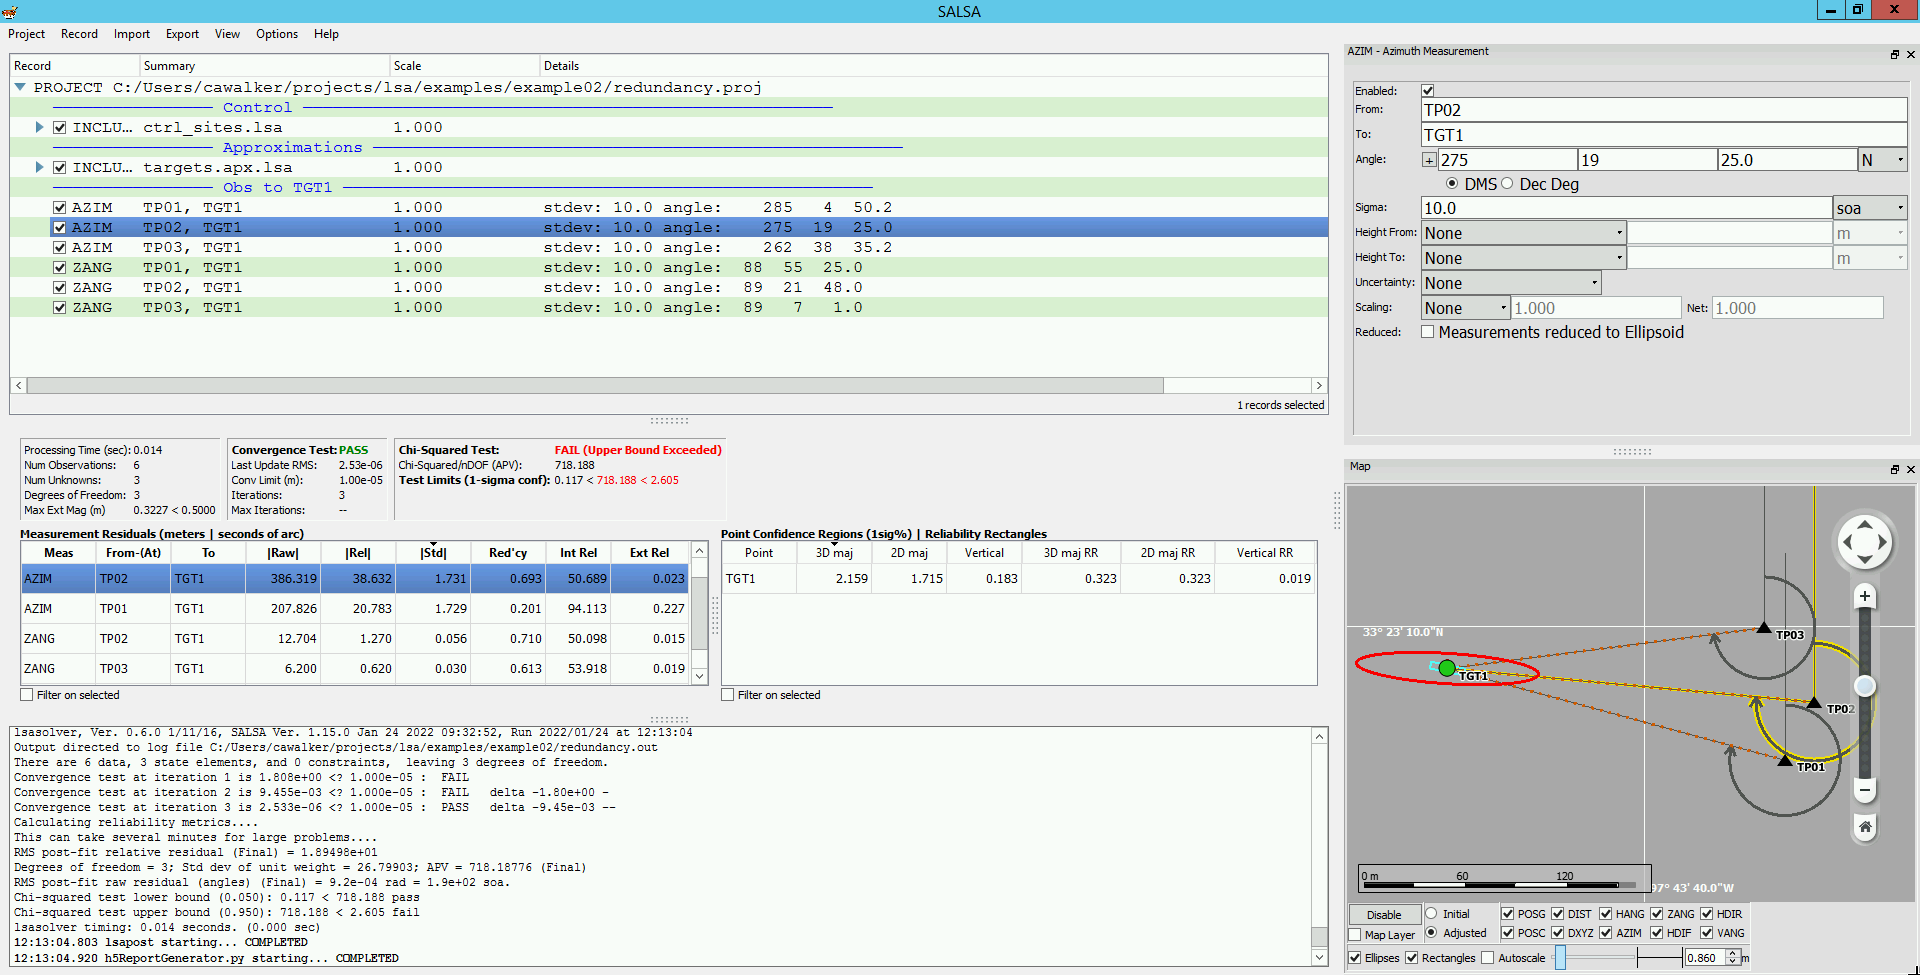
\includegraphics[width=0.99\textwidth]{example02/with_redundancy}
\end{center}
\caption{Reliability rectangle with AZIM record re-enabled (3-point intersection).  Note the scale of the map shows the rectangle is sub-meter.}
\label{fig:ex02redundrectangle}
\end{figure}

For completeness, and to satisfy our desire to resolve the blunder in this survey, correct the blunder in the AZIM record (TP02 to TGT1), restoring the minutes field from 19 back to 10.  Re-run the adjustment.  All tests should pass, and both the point confidence region and reliability rectangle should be sub-meter, as shown in Figure \ref{fig:ex02resolved}.

\begin{figure}[!htbp]
\begin{center}
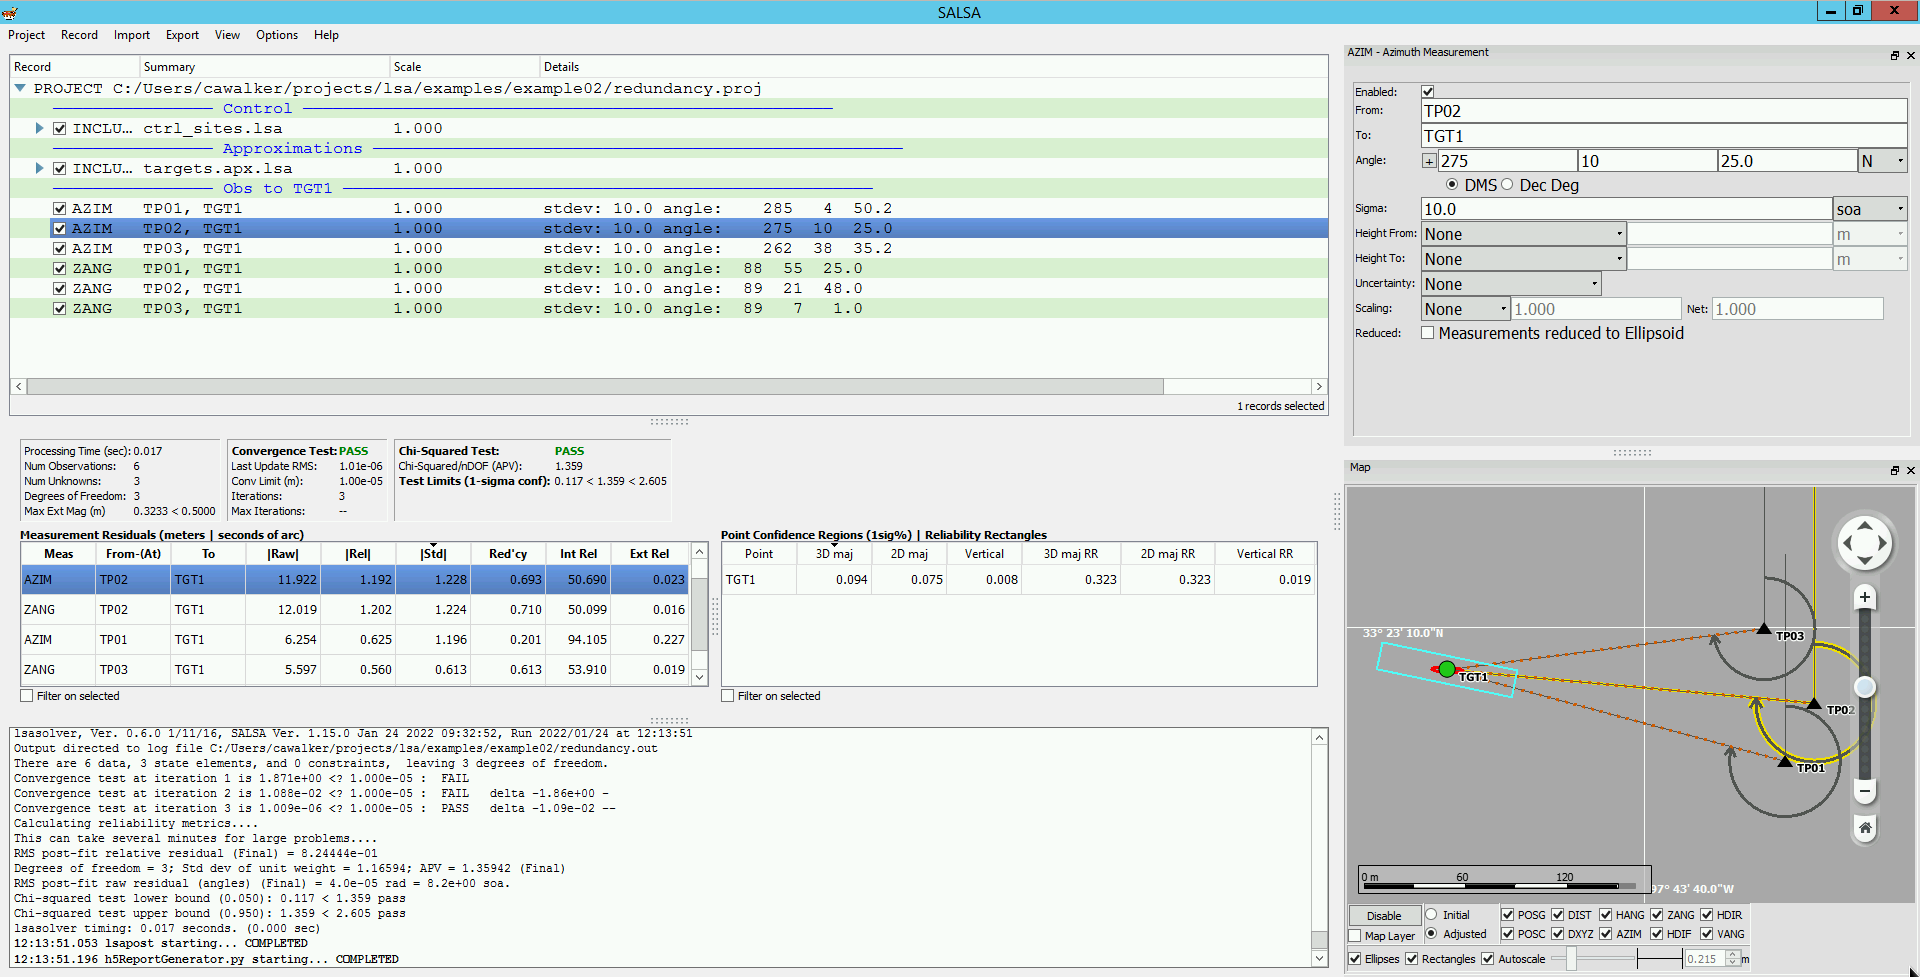
\includegraphics[width=0.99\textwidth]{example02/resolved}
\end{center}
\caption{Adjustment result with blunder resolved.  Note the ellipse and rectangle show the precision and reliability, respectively, are sub-meter.}
\label{fig:ex02resolved}
\end{figure}

In summary, just as the point confidence regions and ellipses help quantify and visualize the precision achieved through the survey and adjustment, the reliability metrics and rectangles help quantify and visualize the sensitivity of those results to a single undetectable error.  In order to assert confidence in a survey result, the surveyor must ensure that the survey design includes sufficient redundancy to meet both the precision and reliability goals as demanded by their application.

\newpage

\section{Example 3: 1D Adjustment (Leveling) Workflow}
A commonly encountered problem in survey is the need to run an adjustment on a leveling line.  These adjustments are special since they typically are devoid of any measurements which could be used to determine the horizontal position of a point. (Note: Project data for this example were constructed from \cite{ngsSlopeSurvey}). Consider the following project initially consisting of one fixed point and two points fixed in latitude and longitude. Since we will only be incorporating leveling data, it is important that our unknown points be fixed in latitude and longitude so that the problem is not underdetermined. Create POSG records utilizing the information in Table \ref{tab:POSGleveling} below.

\begin{table}[htb]
\caption{POSG Record Values}
\vspace{-0.4 cm}
\label{tab:POSGleveling}
\begin{center}
\resizebox{\textwidth}{!}
{\begin{tabular}{ccccc}
	\hline
	\textbf{Point} &\textbf{Status} &\textbf{Lat (N)} &\textbf{Lon (W)} &\textbf{Orthometric Hgt(m)} \\
	\hline
	AUSTIN CE & Fixed & 30 16 48.06083 & 97 44 16.33828 & 160.1613 \\
	N2277258 & Lat/Lon Fixed & 30 16 48.03800 & 97 43 48.14953 & 0.0000 \\
	A 1521 & Lat/Lon Fixed & 30 16 49.57966 & 97 43 0.43960 & 0.0000 \\
	\hline
\end{tabular}}
\end{center}
\end{table}

We will now incorporate the set of HDIF measurements from our fixed station to the stations whose heights we want to estimate. Locate the \verb+example\example03+ subdirectory and copy its contents into the current project folder. Utilizing the Import $\to$ Include from LSA... menu action, go ahead and select the file \verb+loop1.lsa+. At this point, go ahead and expand the records under the \verb+loop1.lsa+ Include record. The \verb+hdiffsAB.lsa+ contains HDIF records starting at AUSTIN CE and going to N2277258, while the \verb+hdiffsBA.lsa+ Include record contains HDIF records working in the opposite direction. 

At this point, the user may have noticed that in each .lsa record that only two points have latitude and longitude information associated with them. The rest only have HDIF records. Normally, this would cause the problem to be underdetermined. However, SALSA is fully capable of handling 1-D leveling lines. As a demonstration, go ahead and disable the \verb+hdiffsBA.lsa+ Include and A 1521 POSG records. Hit the Home key in the Map widget to refresh the view, then select the menu action Project $\to$ Generate Initial Positions and when prompted select Save. 

The user can now observe the appearance of the temporary leveling points between AUSTIN CE and N2277258 in Figure \ref{Fig:AprioriLeveling}. Zooming in on the map it can be seen that the temporary points are chained together based on the set of HDIF records they are associated with. Further inspection in the Auto-Generated Initial Coordinates shows that SALSA has made an initial estimate of the Latitude and Longitude for these temporary points and fixed those two values as well. SALSA has a special treatment for 1-D leveling lines. As the temporary points can not be estimated by most of the a priori algorithms, if SALSA detects a collection of points joined together by HDIF records, it will estimate their latitudes and longitudes by evenly spacing the points between the estimated endpoints. Once those estimates are obtained, their latitude and longitudes will be fixed so that the solver can compute unique solutions for these points in 3D space. The estimation of these values serves mostly as a sanity check so that the user can ensure the leveling line is appropriate. For more detailed information on how leveling lines are drawn, refer to the Leveling Loop Formation and Side Shot Handling discussions of section \ref{sec:apriorisection}.

\begin{figure}[H]
	\begin{center}
		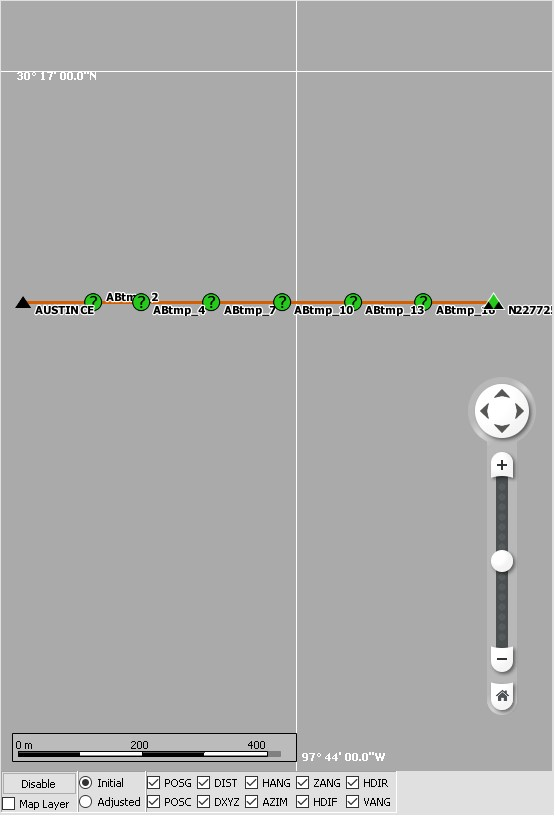
\includegraphics[height=0.50\textheight]{oneDLevelingAPriori.png}
	\end{center}
	\caption{Leveling line generated from HDIF record set.}
	\label{Fig:AprioriLeveling}
\end{figure}

Now let's return to the crux of the exercise and solve for the unknown heights of our sites. Re-enable the \verb+hdiffsBA.lsa+ and A 1521 records, then choose the menu action Import $\to$ Include from LSA... and select \verb+loop2.lsa+ when prompted. The reported sigmas on our HDIF records trend more optimistic than conservative. This will be accounted for by creating a UNCR record with label hdifUNCR and sigma value of 0.0001 m. Once the UNCR record is created, multi select all HDIF records and choose hdifUNCR from the Uncertainty dropdown box. Select the menu action Project $\to$ Calculate Adjustment and save when prompted. The reported orthometric heights (recorded in Table \ref{tab:FinalHeightValues} below) can be observed by choosing the action View $\to$ Final Positions. With no a priori knowledge of our heights, the solver was able to provide an estimate utilizing a collection of HDIF records.

\begin{table}[H]
\caption{Final Height Values}
\label{tab:FinalHeightValues}
\begin{center}
\begin{tabular}{|cc|}
	\hline
	\textbf{Point} &\textbf{Orthometric Hgt(m)}\\
	\hline
	N2277258 & 178.3720 \\
	A 1521 & 177.5100 \\
	\hline
\end{tabular}
\end{center}
\end{table}

\section{Example 4: 2D Adjustment (Horizontal) Workflow}

Sometimes it is desirable to perform a 2D adjustment, in which the only measurements present are those which constrain the horizontal positions.  These adjustments are special since they typically are devoid of any measurements which could be used to determine the height of a point.  In this section we briefly discuss how to perform horizontal adjustments in \textsf{salsa}.

If there are already POSG or POSC records for all points in the horizontal only project, the user may proceed to mark them all as constrained in height or fixed.  Note that these settings may be toggled with multiple POSG and POSC records selected. %  If apriori positions need to be generate, the user should proceed with the following steps:

\subsection{Example}

Consider the following project consisting of two locations, A and B, in which A is fixed and B is constrained and the geoid is specified to be None.  This network is depicted in Figure \ref{Fig:Hor_ex1}.

\begin{table}
\centering
\begin{tabular}{|ccccc|}\hline
\textbf{Point}&\textbf{Status}&\textbf{Lat}&\textbf{Lon (W)}&\textbf{Hgt}\\
A&Fixed&0&0&0\\
B&Height Constrained&0&-1&0\\\hline
\textbf{Meas}&\textbf{From}&\textbf{To}&\textbf{Value}&\textbf{Uncr}\\
AZIM&A&B&89$^o$ 59' 59''&10''\\
AZIM&A&B&90$^o$  0'  1''&10''\\
DIST&A&B&111.1783 km&1 km\\\hline
\end{tabular}
\end{table}

\begin{figure}
\centering
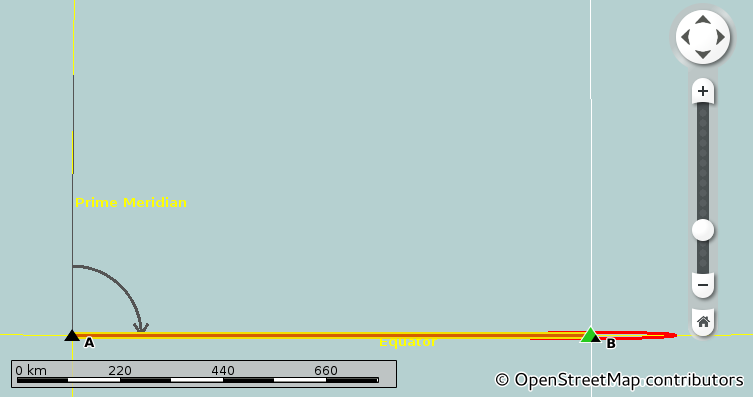
\includegraphics[width=0.9\textwidth]{Hor_ex1.png}
\label{Fig:Hor_ex1}
\caption{A simple horizontal example with two points and two AZIM records.  Note that point B must be constrained in the height since there are no measurements which would allow \textsf{salsa} to determine the height.}
\end{figure}

The point B must be constrained in height for the problem not to be underdetermined.  In \textsf{GeoLab}, this constraining was automatically done for the user, converting points to status 001 instead of 000.  However, \textsf{salsa} does not automatically change the settings so the user is responsible for this step.

The adjustment depicted will execute in \textsf{salsa}, yielding the results displayed in Table \ref{Table:Hor_ex0}.  The results are consistent with the adjustment results one would obtain from \textsf{GeoLab}.

\begin{table}
\centering
\label{Table:Hor_ex0}
\begin{tabular}{|ccc|}\hline
\textbf{Program}&\textbf{B Final Latitude (N,dms)}&\textbf{B Final Longitude (E,dms)}\\\hline
\textsf{salsa}&0$^o$ 0' 0''&0$^o$ 59' 55.4795''\\
\textsf{GeoLab}&0$^o$ 0' 0''&0$^o$ 59' 55.47950''\\\hline
\end{tabular}
\end{table}








\chapter{Supported Measurement Corrections}
\label{chap:corrections}
There are a number of corrections implemented in SALSA which may be used to modify the measurement data of the user.  For convenience, we have tabulated which corrections apply to which record types in the Table \ref{tab:corrections}.
\begin{table}[!htbp]
\centering
\begin{tabular}{|l|c|c|c|c|c|c|c|c|c|c|}\hline
\tiny{\textbf{Record Type}}&\tiny{\textbf{Curv}}&\tiny{\textbf{Hgt}}&\tiny{\textbf{Reduced}}&\tiny{\textbf{Refract}}&\tiny{\textbf{OHC}}\\\hline
\tiny{\textbf{AZIM}}&&\tiny{\textbf{X}}&\tiny{\textbf{X}}&&\\\hline
\tiny{\textbf{DIST}}&&\tiny{\textbf{X}}&&&\\\hline
\tiny{\textbf{DXYZ}}&&\tiny{\textbf{X}}&&&\\\hline
\tiny{\textbf{HANG}}&&\tiny{\textbf{X}}&\tiny{\textbf{X}}&&\\\hline
\tiny{\textbf{HDIF}}&\tiny{\textbf{X}}&&\tiny{\textbf{X}}&\tiny{\textbf{X}}&\tiny{\textbf{X}}\\\hline
\tiny{\textbf{VANG}}&&\tiny{\textbf{X}}&\tiny{\textbf{X}}&\tiny{\textbf{X}}&\\\hline
\tiny{\textbf{ZANG}}&&\tiny{\textbf{X}}&\tiny{\textbf{X}}&\tiny{\textbf{X}}&\\\hline
\end{tabular}
\caption{Table indicating which types of corrections may be applied to which type of record.}
\label{tab:corrections}
\end{table}
\section{Measurement Records}
\subsection{AZIM: Azimuthal Angles} \label{subsection:AZIM}
The azimuth angle record between two points is nominally defined as
\begin{equation}
\text{AZIM} = \underbrace{\f{\pi}{2}-\tan^{-1}\left(\f{\Delta N}{\Delta E}\right)}_{\text{Nominal}}+\text{Corr}_{\text{Hgt}}+\text{Corr}_{\text{DoV}}.
\end{equation}
We have denoted the northernly displacement by $\Delta N$ and the eastwardly displacement by $\Delta E$.
\subsection{DIST: Distance Measurement} \label{subsection:DIST}
The distance measurement is nominally computed as the Pythagorean distance between the two points
\begin{equation}
\text{DIST} = \underbrace{\sqrt{\left(X_{\text{To}}-X_{\text{From}}\right)^2+\left(Y_{\text{To}}-Y_{\text{From}}\right)^2+\left(Z_{\text{To}}-Z_{\text{From}}\right)^2}}_{\text{Nominal}}\times\text{Corr}_{\text{\text{Hgt}}}.
\end{equation}
\subsection{DXYZ: 3-D XYZ Coordinate Difference} \label{subsection:DXYZ}
In ECEF XYZ coordinates, the difference in coordinates is nominally given as
\begin{equation}
\text{DXYZ}=\left(\begin{array}{c}\Delta X\\\Delta Y\\\Delta Z\end{array}\right) = \underbrace{\left(\begin{array}{c}\left(X_{\text{To}}-X_{\text{From}}\right)\\\left(Y_{\text{To}}-Y_{\text{From}}\right)\\\left(Z_{\text{To}}-Z_{\text{From}}\right)\end{array}\right)}_{\text{Nominal}}+\left(\begin{array}{c}\text{Corr}_{\text{Hgt},X}\\\text{Corr}_{\text{Hgt},Y}\\\text{Corr}_{\text{Hgt},Z}\end{array}\right).
\end{equation}
\subsection{HANG: Horizontal Angle}
The horizontal angle between two points may be nominally rewritten (see Figure \ref{Fig:HANG}) as the difference in azimuthal angles between those two points as follows,
\begin{equation}
\text{HANG}=\underbrace{\left(\text{AZIM}_{\text{To,At}}-\text{AZIM}_{\text{From,At}}\right)}_{\text{Nominal}}+\text{Corr}_{\text{Hgt}}+\text{Corr}_{\text{DoV}}.
\end{equation}
\begin{figure}[!htbp]
\centering
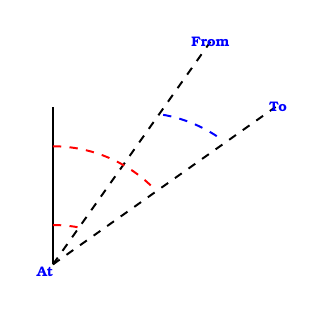
\begin{tikzpicture}
\draw (-0.1,-0.1) node{{\color{blue}{\tiny{\textbf{At}}}}};

\draw[straight,color=black,line width=0.25mm] (0,0) -- (0,2);
\draw[straight,color=black,line width=0.25mm,dashed] (0,0) -- (2,2*1.414) node{{\color{blue}{\tiny{\textbf{From}}}}};
\draw[straight,color=black,line width=0.25mm,dashed] (0,0) -- (2*1.414,2) node{{\color{blue}{\tiny{\textbf{ To}}}}};
\draw[color=red,line width=0.25mm,dashed] (0,0.5) arc (90:80:1.8);
\draw[color=red,line width=0.25mm,dashed] (0,1.5) arc (90:45:1.8);
\draw[color=blue,line width=0.25mm,dashed] (1.4,1.9) arc (80:55:1.8);
\end{tikzpicture}
\caption{Horizontal angle measurements may be thought of as the difference of two azimuthal angle measurements.}
\label{Fig:HANG}
\end{figure}
\subsection{HDIF: Height Difference} \label{subsection:HDIF}
The difference in ellipsoidal heights is nominally given as
\begin{eqnarray*}
\text{HDIF} &=& \underbrace{\left(h_{\text{To}}-h_{\text{From}}\right)}_{\text{Nominal}}\\
&=&\left(H_{\text{To}}-H_{\text{From}}\right)+\left[\left(\text{Geoid Height}\right)_{\text{To}}-\left(\text{Geoid Height}\right)_{\text{From}}\right]\\
&& + \text{Corr}_{\text{Curv}} + \text{Corr}_{\text{Reduced}} + \text{Corr}_{\text{Refrac}} + \text{Corr}_{\text{OHC}}.
\end{eqnarray*}
By default, it is assumed that the user has input an orthometric height difference.
\subsection{VANG: Vertical Angle} \label{subsection:VANG}
The vertical angle is given trigonometrically (see Figure \ref{Fig:VANG}) by
\begin{equation}
\text{VANG} =\underbrace{\sin^{-1}\left(\f{\Delta U}{D}\right)}_{\text{Nominal}}+\text{Corr}_{\text{Hgt}}+\text{Corr}_{\text{DoV}}+\text{Corr}_{\text{Refrac}}.
\end{equation}
Here $\Delta U$ denotes the up displacement between the ``To'' site and the ``From'' site.  The Pythagorean slant distance is denoted by $D$.
\begin{figure}[!htbp]
\centering
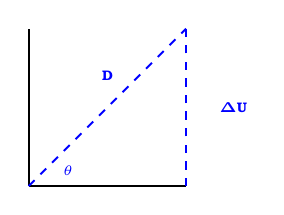
\begin{tikzpicture}
\draw (1,1.4) node{{\color{blue}{\tiny{\textbf{D}}}}};
\draw (2.6,1) node{{\color{blue}{\tiny{$\mathbf{\Delta}$\textbf{U}}}}};
\draw (0.5,0.2) node{{\color{blue}{\tiny{$\theta$}}}};

\draw[straight,color=black,line width=0.25mm] (0,0) -- (2,0);
\draw[straight,color=black,line width=0.25mm] (0,0) -- (0,2);
\draw[straight,color=blue,line width=0.25mm,dashed] (0,0) -- (2,2);
\draw[straight,color=blue,line width=0.25mm,dashed] (2,0) -- (2,2);
\end{tikzpicture}
\caption{The vertical angle is trigonometrically related to the upwardly displacement $\Delta U$ and the Pythagorean slant distance $D$.}
\label{Fig:VANG}
\end{figure}
\subsection{ZANG: Zenith Angle}
The zenith angle is the complement angle to the vertical elevation angle.  Therefore we obtain
\begin{equation}
\sin\left(\text{VANG}\right)=\sin\left(\f{\pi}{2}-\text{ZANG}\right)=\cos\left(\text{ZANG}\right).
\end{equation}
This results in 
\begin{equation}
\text{ZANG}=\underbrace{\cos^{-1}\left(\f{\Delta U}{D}\right)}_{\text{Nominal}}+\text{Corr}_{\text{Hgt}}+\text{Corr}_{\text{DoV}}+\text{Corr}_{\text{Refrac}}.
\end{equation}
\section{Curvature}
In this section we will discuss the curvature correction.  This correction is enabled by default, but if your instrument is configured to perform the corrections itself this option should be disabled.
\subsection{HDIF: Height Difference}
When this option is applied to HDIF records, the height difference arising from the curvature of the Earth is approximated and removed.  Begin by noting that the geometry of the problem displayed in Figure \ref{Fig:Curv} implies the following relationship (utilizing the small angle approximation)
\begin{equation}
\alpha \approx \f{\Delta H}{D} \approx \f{(D/2)}{R_{\text{Earth}}}.
\end{equation}

\begin{figure}[!htbp]
\centering
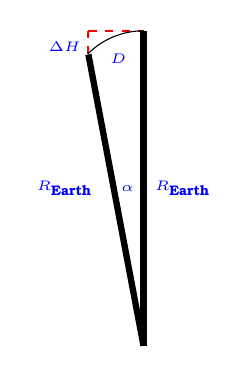
\begin{tikzpicture}
\draw (-1.,2) node{{\color{blue}{\tiny{\textbf{$R_{\text{Earth}}$}}}}};
\draw (0.5,2) node{{\color{blue}{\tiny{\textbf{$R_{\text{Earth}}$}}}}};
\draw (-1.,3.8) node{{\color{blue}{\tiny{\textbf{$\Delta H$}}}}};
\draw (-0.32,3.65) node{{\color{blue}{\tiny{\textbf{$D$}}}}};
\draw (-0.2,2) node{{\color{blue}{\tiny{\textbf{$\alpha$}}}}};

\draw[straight,color=black,line width=0.8mm] (0,0) -- (-0.7,3.7);
\draw[straight,color=red,line width=0.25mm,dashed] (-0.7,3.7) -- (-0.7,4);
\draw[straight,color=red,line width=0.25mm,dashed] (-0.7,4) -- (0,4);
\draw[straight,color=black,line width=0.8mm] (0,0) -- (0,4);
\draw (0,4) arc (90:135:1);

\end{tikzpicture}
\caption{The curvature correction to the height difference may be directly found from geometric considerations.}
\label{Fig:Curv}
\end{figure}
We may solve this for the change in orthometric height to obtain
\begin{equation}
\text{Corr}_{\text{Curv}} = (-\Delta H) = -\f{D^2}{2R_{\text{Earth}}}.
\end{equation}
We have introduced the slant distance, $D$, which is the Pythagorean distance between the two points.  Note, one recovers (5.4) of \cite{anderson} if $R_{\text{Earth}}$ is taken to be $6371$ km.

\section{Height Corrections}
In this section we will discuss the corrections which arise due to the height of the instrument and/or the target position.
\subsection{AZIM Records}
There is a correction arising from the geodetic height of the target position.  The correction is of the form\footnote{For further details, we refer the reader to \cite{Burkholder97} or (23.33) of \cite{ghilani}.}
\begin{equation}
\text{Corr}_{\text{Hgt}}\approx\left(\f{0.108''}{1000}\right)h_{\text{To,Geodetic}}\cos^2\left(\phi_{\text{From}}\right)\sin\left(2\cdot\text{AZIM}_{\text{To,From}}\right).
\end{equation}

\subsection{DIST Records} \label{subsection:DIST_HeightCorrection}
When this option is applied to DIST records, the contribution to the distance from the instrument and target height is removed.  The general strategy is to reduce the measurement to the ellipsoid and then to recompute the slant distance.  The resulting form of the correction is \cite{Ghilani_dist_reduced}.
\begin{equation}\label{eq:dist_hgt}
\text{Corr}_{\text{Hgt}}=\sqrt{\left[1-\left(\f{h_{2,\text{tot}}-h_{1,\text{tot}}}{\text{Nominal}}\right)^2\right]\f{\left(R_{\text{Earth}}+h_2\right)\left(R_{\text{Earth}}+h_1\right)}{\left(R_{\text{Earth}}+h_{2,\text{tot}}\right)\left(R_{\text{Earth}}+h_{1,\text{tot}}\right)}+\left(\f{h_2-h_1}{\text{Nominal}}\right)^2}.
\end{equation}
We have let $h_{1,\text{tot}}$ and $h_{2,\text{tot}}$ denote the sum of the ellipsoidal height and the height offset at that point.

To easily derive this result, consider the geometry presented in Figure \ref{Fig:triangles}.

\begin{figure}[!htbp]
\centering
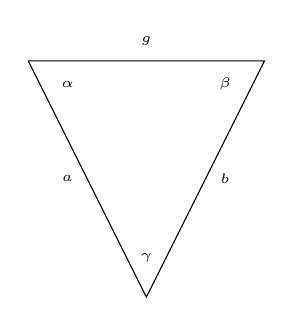
\begin{tikzpicture}
\draw (0,3)--(3,3)--(1.5,0)--(0,3);
\draw (0.5,2.7) node{{\color{black}{\tiny{\textbf{$\alpha$}}}}};
\draw (2.5,2.7) node{{\color{black}{\tiny{\textbf{$\beta$}}}}};
\draw (1.5,0.5) node{{\color{black}{\tiny{\textbf{$\gamma$}}}}};
\draw (1.5,3.25) node{{\color{black}{\tiny{\textbf{$g$}}}}};
\draw (0.5,1.5) node{{\color{black}{\tiny{\textbf{$a$}}}}};
\draw (2.5,1.5) node{{\color{black}{\tiny{\textbf{$b$}}}}};
\end{tikzpicture}~~~~~~~~~~
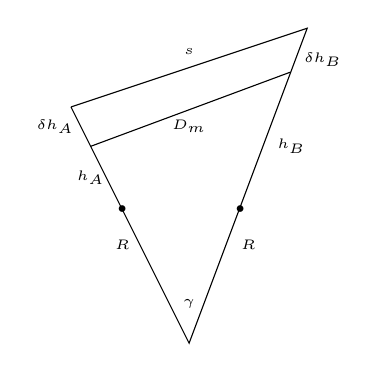
\begin{tikzpicture}
\draw (0,3)--(3,4)--(1.5,0)--(0,3);
\draw (0.25,2.5)--(2.78,3.44);
\draw (1.5,0.5) node{{\color{black}{\tiny{\textbf{$\gamma$}}}}};
\draw (1.5,3.71) node{{\color{black}{\tiny{\textbf{$s$}}}}};
\draw (1.5,2.75) node{{\color{black}{\tiny{\textbf{$D_m$}}}}};
\draw (0.65,1.7) node{{\color{black}{\tiny{\textbf{$\bullet$}}}}};
\draw (2.15,1.7) node{{\color{black}{\tiny{\textbf{$\bullet$}}}}};
\draw (0.65,1.25) node{{\color{black}{\tiny{\textbf{$R$}}}}};
\draw (2.25,1.25) node{{\color{black}{\tiny{\textbf{$R$}}}}};
\draw (0.25,2.1) node{{\color{black}{\tiny{\textbf{$h_A$}}}}};
\draw (2.8,2.5) node{{\color{black}{\tiny{\textbf{$h_B$}}}}};
\draw (-0.2,2.75) node{{\color{black}{\tiny{\textbf{$\delta h_{A}$}}}}};
\draw (3.2,3.6) node{{\color{black}{\tiny{\textbf{$\delta h_{B}$}}}}};
\end{tikzpicture}
\caption{Geometry relevant for law of cosines discussion (left) and for height correction derivation (right).  We have used $s$ to denote the nominal slant distance and $D_m$ to denote the mark-to-mark distance.}
\label{Fig:triangles}
\end{figure}
Recall that the law of cosines may be written as
\begin{equation}
g^2=a^2+b^2-2ab\cos\gamma = (a-b)^2+4ab\sin\f{\gamma}{2}.
\end{equation}
Applying the law of cosines to the geometry relevant for the correction yields
\begin{eqnarray}
s^2 = (h_{B,\text{tot}}-h_{A,\text{tot}})^2+4(R+h_{A,\text{tot}})(R+h_{B,\text{tot}})\sin\f{\gamma}{2},\\
D_m^2 = (h_{B}-h_{A})^2+4(R+h_{A})(R+h_{B})\sin\f{\gamma}{2}.
\end{eqnarray}
Combining these results yields
\begin{equation}
D_m^2 = \left(s^2-(h_{B,\text{tot}}-h_{A,\text{tot}})^2\right)\f{(R+h_A)(R+h_B)}{(R+h_{A,\text{tot}})(R+h_{B,\text{tot}})}+(h_B-h_A)^2.
\end{equation}
Factoring out the nominal slant distance, $s$, results in equation \eqref{eq:dist_hgt}.
\subsection{DXYZ Records}
When this option is applied to DXYZ records, the XYZ coordinates at each point are adjusted for the specified heights.  The height offsets at each of the points is transformed into a height offset in XYZ coordinates by
\begin{equation}
\left[\begin{array}{c}(\Delta X)_{\text{From}}\\(\Delta Y)_{\text{From}}\\(\Delta Z)_{\text{From}}\end{array}\right]=R_{\text{ENU2XYZ},{\text{From}}}\cdot\left[\begin{array}{c}0\\0\\h_{\text{offset},\text{From}}\end{array}\right],\hspace*{4mm}\left[\begin{array}{c}(\Delta X)_{\text{To}}\\(\Delta Y)_{\text{To}}\\(\Delta Z)_{\text{To}}\end{array}\right]=R_{\text{ENU2XYZ},{\text{To}}}\cdot\left[\begin{array}{c}0\\0\\h_{\text{offset},\text{To}}\end{array}\right].
\end{equation}
The correction to the DXYZ measurement (which subtracts off the difference due to the instrument and target height offset) may be written as
\begin{equation}
\text{Corr}_{\text{Hgt},XYZ}=-\left[\begin{array}{c}\left(\Delta X\right)_{\text{To}}-\left(\Delta X\right)_{\text{From}}\\\left(\Delta Y\right)_{\text{To}}-\left(\Delta Y\right)_{\text{From}}\\\left(\Delta Z\right)_{\text{To}}-\left(\Delta Z\right)_{\text{From}}\end{array}\right].
\end{equation}
\subsection{HANG Records}
Since we have written the horizontal angle as the difference of two azimuthal angles (see Figure \ref{Fig:HANG}), the target site height correction is likewise the difference of two azimuthal corrections
\begin{equation}
\text{Corr}_{\text{Hgt}}=\left(\f{0.108''}{1000}\right)\cos^2\left(\phi_{\text{At}}\right)\left[h_{\text{To,Geodetic}}\sin\left(2\cdot\text{AZIM}_{\text{To,At}}\right)-h_{\text{From,Geodetic}}\sin\left(2\cdot\text{AZIM}_{\text{From,At}}\right)\right].
\end{equation}
\subsection{VANG Records}
The correction to the VANG measurement may be written as
\begin{equation}
\left(\text{Nominal}\right) + \text{Corr}_{\text{Hgt}}\approx\tan^{-1}\left[\tan\left(\text{Nominal}\right)-\left(\f{\Delta h_{\text{specified}}}{\text{slant distance}}\right)\right].
\end{equation}
\subsection{ZANG Records}
The corrected ZANG record is the complementary angle to the corrected VANG record,
\begin{equation}
\left(\text{Nominal}\right)+\text{Corr}_{\text{Hgt}}\approx\f{\pi}{2}-\left[\tan^{-1}\left[\tan\left(\f{\pi}{2}-\text{Nominal}\right)-\left(\f{\Delta h_{\text{specified}}}{\text{slant distance}}\right)\right]\right].
\end{equation}
\section{Reduced to Ellipsoid}
In this section we will discuss the option of reducing your measurements to the ellipsoid.  This removes all geoid-related corrections from your measurements.  This usually takes the form of preventing deflection of vertical corrections from being applied.  The two deflection of vertical components are given by
\begin{equation}
\begin{split}
\xi\hspace*{2mm}\left(\text{North--South Direction}\right)&=\Phi-\phi,\\
\eta\hspace*{2mm}\left(\text{East--West Direction}\right)&=\left(\Lambda-\lambda\right)\cos\phi.
\end{split}
\end{equation}
The symbols $\left\{\phi,\lambda\right\}$ denote the ellipsoidal latitude and longitude.  The symbols $\left\{\Phi,\Lambda\right\}$ denote the astronomical latitude and longitude.

In order to relate this to the language of North--South and East--West, consider the following:\\
$(\xi<0)$: A negative meridian component (MC) of Deflection of the Vertical (DoV) indicates that the astronomic latitude ($\Phi$) will fall to the south of the corresponding geodetic latitude ($\phi$) of the point.\\
$(\eta<0)$: A negative prime vertical component (PVC) of the Deflection of the Vertical (DoV) indicates that the astronomic longitude ($\Phi$) will fall to the west of the corresponding geodetic longitude ($\lambda$) of the point.

In SALSA, these parameters are computed by noting that
\begin{equation}
\begin{split}
\tan\hspace{1mm}\xi&=-\f{\partial\left(\text{Geoid Height}\right)}{\partial\left(\text{North}\right)}=-\f{1}{\text{R}_{\text{Earth}}}\f{\partial\left(\text{Geoid Height}\right)}{\partial\phi},\\
\tan\hspace*{1mm}\eta&=-\f{\partial\left(\text{Geoid Height}\right)}{\partial\left(\text{East}\right)}=-\f{1}{\text{R}_{\text{Earth}}\cos\left(\phi\right)}\f{\partial\left(\text{Geoid Height}\right)}{\partial\lambda}.
\end{split}
\end{equation}
Note that the final forms on the right hand side agree with equation (6.184) of \cite{torge} after noting that $\tan\hspace*{1mm}\theta\approx\theta$ for small $\theta$.

\subsection{AZIM Records}
When this option is applied to AZIM records, the deflection of vertical corrections are not included.  There are two contributions from the deflection of vertical on the azimuthal angle.  The final expression for the change in azimuthal angle is given by\footnote{We refer the user to (5--98) of \cite{wellenhof} for further details.}
\begin{equation}
\text{Corr}_{\text{DoV}}=-\eta_{\text{From}}\tan\phi_{\text{From}}-\left[\xi_{\text{From}}\sin\left(\text{AZIM}_{\text{To,From}}\right)-\eta_{\text{From}}\cos\left(\text{AZIM}_{\text{To,From}}\right)\right]\cot\left(\text{ZANG}_{\text{To,From}}\right).
\end{equation}
\subsection{HANG Records}
This prevents the deflection of vertical correction from being applied.  Since we have written the horizontal angle as the difference of two azimuthal angles (see Figure \ref{Fig:HANG}), the deflection of vertical correction is likewise the difference of two azimuthal deflection of vertical corrections.  Those corrections takes the form
\begin{equation}
\begin{split}
\text{Corr}_{\text{DoV}}&=\left\{-\left[\xi_{\text{At}}\sin\left(\text{AZIM}_{\text{To,At}}\right)-\eta_{\text{At}}\cos\left(\text{AZIM}_{\text{To,At}}\right)\right]\cot\left(\text{ZANG}_{\text{To,At}}\right)\right.\\
&\left.+\left[\xi_{\text{At}}\sin\left(\text{AZIM}_{\text{From,At}}\right)-\eta_{\text{At}}\cos\left(\text{AZIM}_{\text{From,At}}\right)\right]\cot\left(\text{ZANG}_{\text{From,At}}\right)\right\}.
\end{split}
\end{equation}
\subsection{HDIF Records}
When the this option is applied to HDIF records, the accounting for the geoid heights is removed,
\begin{equation}
\text{Corr}_{\text{Reduced}} = -\left[\left(\text{Geoid Height}\right)_{\text{To}}-\left(\text{Geoid Height}\right)_{\text{From}}\right].
\end{equation}
\subsection{VANG Records}
When this option is applied to VANG records, the deflection of vertical corrections are not included.  Those corrections take the form
\begin{equation}
\text{Corr}_{\text{DoV}}=-\left[\xi_{\text{From}}\cos\left(\text{AZIM}_{\text{To,From}}\right)+\eta_{\text{From}}\sin\left(\text{AZIM}_{\text{To,From}}\right)\right].
\end{equation}
\subsection{ZANG Records}
When this option is applied to ZANG records, the deflection of vertical corrections are not included.  Those corrections takes the form (see Figure \ref{Fig:ZANG_DOV})
\begin{equation}
\text{Corr}_{\text{DoV}}=\left[\xi_{\text{From}}\cos\left(\text{AZIM}_{\text{To,From}}\right)+\eta_{\text{From}}\sin\left(\text{AZIM}_{\text{To,From}}\right)\right].
\end{equation}
This correction agrees with (5--101) of \cite{wellenhof}.
\begin{figure}[!htbp]
\centering
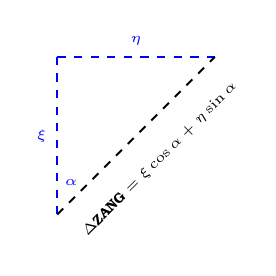
\begin{tikzpicture}
\draw (0.175,0.4) node{{\color{blue}{\tiny{\textbf{$\alpha$}}}}};
\draw (1.3,0.7) node{{\color{black}{\tiny{\textbf{\rotatebox{45}{$\Delta \text{ZANG}=\xi\cos\alpha+\eta\sin\alpha$}}}}}};
\draw (1,2.2) node{{\color{blue}{\tiny{\textbf{$\eta$}}}}};
\draw (-0.2,1) node{{\color{blue}{\tiny{\textbf{$\xi$}}}}};

\draw[straight,color=blue,line width=0.25mm,dashed] (0,0) -- (0,2);
\draw[straight,color=blue,line width=0.25mm,dashed] (0,2) -- (2,2);
\draw[straight,color=black,line width=0.25mm,dashed] (0,0) -- (2,2);

\end{tikzpicture}
\caption{The deflection of vertical contribution to the zenith angle may be directly found from geometric considerations.  This is a top down view (looking down the ``Up'' axis) of how a North--South deflection and a East--West deflection result in a zenith angle contribution.}
\label{Fig:ZANG_DOV}
\end{figure}
\section{Refraction}
In this section we will discuss the refraction correction.  Physically, refraction impacts survey measurements by causing light to propagate through a different path length than is anticipated by the surveyor (light ``bends'' to a target as opposed to traveling in a straight-line).
\subsection{HDIF Records}
When this option is applied to HDIF records, vertical refraction is accounted for.  From Figure \ref{Fig:Refrac}, the geometrical relationship between the radius of curvature $r$ and the height difference is given by (utilizing the small angle approximation)
\begin{equation}
\delta \approx \f{\Delta H}{D} \approx \f{(D/2)}{r}.
\end{equation}

\begin{figure}[!htbp]
\centering
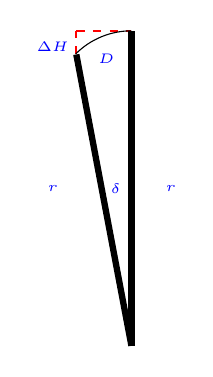
\begin{tikzpicture}
\draw (-1.,2) node{{\color{blue}{\tiny{\textbf{$r$}}}}};
\draw (0.5,2) node{{\color{blue}{\tiny{\textbf{$r$}}}}};
\draw (-1.,3.8) node{{\color{blue}{\tiny{\textbf{$\Delta H$}}}}};
\draw (-0.32,3.65) node{{\color{blue}{\tiny{\textbf{$D$}}}}};
\draw (-0.2,2) node{{\color{blue}{\tiny{\textbf{$\delta$}}}}};

\draw[straight,color=black,line width=0.8mm] (0,0) -- (-0.7,3.7);
\draw[straight,color=red,line width=0.25mm,dashed] (-0.7,3.7) -- (-0.7,4);
\draw[straight,color=red,line width=0.25mm,dashed] (-0.7,4) -- (0,4);
\draw[straight,color=black,line width=0.8mm] (0,0) -- (0,4);
\draw (0,4) arc (90:135:1);

\end{tikzpicture}
\caption{The refraction correction to the height difference may be directly found from geometric considerations.  We have used $r$ to denote the radius of curvature radius and $\delta$ to denote the refraction angle.}
\label{Fig:Refrac}
\end{figure}

We may introduce the refraction coefficient, $k=R_{\text{Earth}}/r$, and solve for the change in height to obtain
\begin{equation}
\text{Corr}_{\text{Refrac}} = (\Delta H) = k\f{D^2}{2R_{\text{Earth}}}.
\end{equation}
We have introduced the slant distance, $D$, which is the Pythagorean distance between the two points.

It is common for sources to give the equation for the combined effect of curvature and refraction.  
\begin{equation}
\begin{split}
\text{Corr}_{\text{Curv}}+\text{Corr}_{\text{Refrac}}&=\left(-1+k\right)\f{D^2}{2R_{\text{Earth}}}\\
&\approx \left(-1+0.14\right)\left(0.0785\right)(D/\text{km})^2\\
&\approx -0.0675 (D/\text{km})^2.
\end{split}
\end{equation}
The numerical values were chosen to demonstrate consistency with (5.7) of \cite{anderson}.  We emphasize that SALSA allows the user to specify the refraction coefficient $k$.

\subsection{VANG Records}
When this option is applied to VANG records, the refraction angle is subtracted from the measured angle.  As shown in Figure \ref{Fig:Refrac}, the added refraction angle may be written as
\begin{equation}
\delta \approx \f{(D/2)}{r}.
\end{equation}
Rewriting this in terms of the refraction coefficient $k=R_{\text{Earth}}/r$ immediately allows us to obtain the contribution which must be removed from the angular measurement
\begin{equation}
\text{Corr}_{\text{Refrac}}=-k\f{D}{2R_{\text{Earth}}}.
\end{equation}
This contribution agrees with (5.12b) of \cite{torge}.
\subsection{ZANG Records}
When this option is applied to ZANG records, it adds the refraction angle to the measurement.  Similarly to the VANG record, we choose to write the refraction angle in terms of the refraction coefficient to obtain
\begin{equation}
\text{Corr}_{\text{Refrac}}=k\f{D}{2R_{\text{Earth}}}.
\end{equation}

\section{Orthometric Height Correction}\label{sec:OHC}
In this section we will discuss the orthometric height correction.
\subsection{HDIF Records}
When this option is applied to HDIF records, the difference in gravitational acceleration between the two points is accounted for.  For brevity, we will use the subscript ``$1$'' in place of ``From'' and the subscript ``$2$'' in place of ``To'' in this section.  The definition of the orthometric height is the integral along the plumb line from the geoid to the surface of the gravitational acceleration divided by the mean gravitational acceleration along the plumb line,\footnote{See (3.106) of \cite{torge}.}
\begin{equation}
H=\f{1}{\bar{g}}\int_{\text{geoid}}^{\text{surface}}g\hspace*{1mm} dn.
\end{equation}
A useful difference to consider is the difference in integrals between the two points
\begin{equation}
\left(\bar{g}_2H_2-\bar{g}_1H_1\right)=\int_{\text{surface}_1}^{\text{surface}_2}g\hspace*{1mm} dn.
\end{equation}
By adding and subtracting by the appropriate factors, we may obtain the expression
\begin{equation}
(H_2-H_1)={\underbrace{\Delta n}_{\text{Leveling}}}+{\underbrace{\int_{\text{surface}_1}^{\text{surface}_2}\left(\f{g-\gamma_0^{45}}{\gamma_0^{45}}\right)dn-\left(\f{\bar{g}_2-\gamma_0^{45}}{\gamma_0^{45}}\right)H_2+\left(\f{\bar{g}_1-\gamma_0^{45}}{\gamma_0^{45}}\right)H_1}_{\text{Corr}_{\text{OHC}}}}.
\end{equation}
We have denoted the level measurement value as $\Delta n$.  The introduced constant, $\gamma_0^{45}$, is the normal gravitational acceleration evaluated on the surface of the ellipsoid and at 45 degrees latitude.  Numerically, this has a value of $\gamma_0^{45}=9.806199$ m/s$^2$.

In practice, the terms which comprise the orthometric height correction are not known.  Therefore Poincare-Prey Reduction\footnote{See section 3.5 of \cite{wellenhof}.} is often utilized to eliminate the mean gravitational acceleration from the expression
\begin{equation}
\bar{g}=g+\left(4.24\times10^{-7}\right)H/\text{s}^2.
\end{equation}

Performing elementary algebra we find the orthometric height correction to be approximately given by\footnote{We have used the Midpoint Rule approximation, $\int_{\text{surface}_1}^{\text{surface}_2}\left(\f{g-\gamma_0^{45}}{\gamma_0^{45}}\right)dn\approx\f{1}{2}\sum_i\left(\f{g_i-\gamma_0^{45}}{\gamma_0^{45}}\right)\left(H_2-H_1\right)$.}
\begin{equation}
\text{Corr}_{\text{OHC}}\approx\f{1}{2}\sum_i\left(\f{g_i-\gamma_0^{45}}{\gamma_0^{45}}\right)\left(H_2-H_1\right)+\left(\f{g_1-\gamma_0^{45}}{\gamma_0^{45}}\right)H_1-\left(\f{g_2-\gamma_0^{45}}{\gamma_0^{45}}\right)H_2-\left(4.317\times10^{-8}\right)(H_2-H_1).
\end{equation}

The gravitational accelerational acceleration usually is not known and therefore the normal gravitational acceleration is used in place of the physical gravitational acceleration,
\begin{equation}
\text{Corr}_{\text{OHC}}\approx\f{1}{2}\sum_i\left(\f{\gamma_i-\gamma_0^{45}}{\gamma_0^{45}}\right)\left(H_2-H_1\right)+\left(\f{\gamma_1-\gamma_0^{45}}{\gamma_0^{45}}\right)H_1-\left(\f{\gamma_2-\gamma_0^{45}}{\gamma_0^{45}}\right)H_2-\left(4.317\times10^{-8}\right)(H_2-H_1).
\end{equation}
The normal gravitational acceleration only depends on the latitude ($\phi$) and the ellipsoidal height ($h$) at the point.  Explicitly, the normal gravitational acceleration is given by
\begin{equation}
\begin{split}
\gamma &= \gamma_0 +\left[-\left(3.0877\times10^{-3}-4.3\times10^{-6}\sin^2\phi\right)(h/\text{km})+\left(7.2\times10^{-7}\right)(h/\text{km})^2\right]\text{m}/\text{s},\\
\gamma_0&=9.780327\left(1+5.3024\times10^{-3}\sin^2\phi-5.8\times10^{-6}\sin^2(2\phi)\right)\text{m}/\text{s}^2.
\end{split}
\end{equation}
Our final expressions agree with (4--46) of \cite{wellenhof}.

A common approximation scheme which is found in the literature is to assume:
\begin{itemize}
\item The orthometric heights are much larger than their difference: $H_2\sim H_1$.
\item The height dependent terms in the normal gravity are negligible: $\gamma\sim\gamma_0$.
\item $\gamma_0\sim9.780327\left(1+5.3024\times10^{-3}\sin^2\phi\right)\text{m}/\text{s}^2.$
\end{itemize}
This leads to
\begin{equation}\label{eq:OHCapprox}
\text{Corr}_{\text{OHC}}\approx-H_1\left(5.288\times10^{-3}\right)\left(\phi_2-\phi_1\right)\sin\left(2\phi_1\right).
\end{equation}
This agrees with equation (23.39) of \cite{ghilani} and equation (5.27) of \cite{anderson}.\footnote{The adjustment resulting from the use of the approximate form is in agreement with the results of GeoLab \cite{geolab}.}  We would like to emphasis that SALSA uses the more accurate expression which was previously introduced.


\chapter{UNCR Record Corrections}
\label{chap:UNCRcorrections}
There are a number of UNCR record corrections implemented in SALSA which may be used to modify the measurement uncertainty data of the user.  For convenience, we have tabulated which corrections apply to which record types in the Table \ref{tab:UNCRcorrections}.  In general, the instrument will be placed at the ``From'' station and the target will be placed at the ``To'' station.  The one exception is HANG, where the instrument is at the ``At'' station and targets are at the ``From'' and ``To'' stations.

\begin{table}[!htbp]
\centering
\begin{tabular}{|l|c|c|c|c|c|c|c|c|c|c|}\hline
\tiny{\textbf{Record Type}}&\tiny{\textbf{At Cent Err}}&\tiny{\textbf{From Cent Err}}&\tiny{\textbf{To Cent Err}}&\tiny{\textbf{PPM}}&\tiny{\textbf{Sigma}}\\\hline
\tiny{\textbf{AZIM}}&&\tiny{\textbf{X}}&\tiny{\textbf{X}}&&\tiny{\textbf{X}}\\\hline
\tiny{\textbf{DGRP}}&&\tiny{\textbf{X}}&\tiny{\textbf{X}}&&\tiny{\textbf{X}}\\\hline
\tiny{\textbf{DIST}}&&\tiny{\textbf{X}}&\tiny{\textbf{X}}&\tiny{\textbf{X}}&\tiny{\textbf{X}}\\\hline
\tiny{\textbf{DXYZ}}&&\tiny{\textbf{X}}&\tiny{\textbf{X}}&\tiny{\textbf{X}}&\tiny{\textbf{X}}\\\hline
\tiny{\textbf{HANG}}&\tiny{\textbf{X}}&\tiny{\textbf{X}}&\tiny{\textbf{X}}&&\tiny{\textbf{X}}\\\hline
\tiny{\textbf{HDIF}}&&&&\tiny{\textbf{X}}&\tiny{\textbf{X}}\\\hline
\tiny{\textbf{VANG}}&&\tiny{\textbf{X}}&\tiny{\textbf{X}}&&\tiny{\textbf{X}}\\\hline
\tiny{\textbf{ZANG}}&&\tiny{\textbf{X}}&\tiny{\textbf{X}}&&\tiny{\textbf{X}}\\\hline
\end{tabular}
\caption{Table indicating which types of UNCR record corrections may be applied to which type of record.  Note that HDIR Records, while unable to have an UNCR record specified directly, may inherit one from their parent DGRP.}
\label{tab:UNCRcorrections}
\end{table}

\section{Centering Errors and PPM}
Note that centering errors in SALSA are treated as horizontal errors.
\subsection{AZIM: Azimuthal Angles}
The error applied to AZIM measurement records due to Centering Errors takes the following form
\begin{equation}
\label{Eqn:AZIM_Cent}
\sigma_{\text{AZIM,Centering}}^2=\left(\f{\sigma_{\text{From Centering Error}}}{\text{D}_{\text{To, From}}}\right)^2+\left(\f{\sigma_{\text{To Centering Error}}}{\text{D}_{\text{To, From}}}\right)^2.
\end{equation}
Where $\text{D}$ is the horizontal distance, not the slant distance, between the ``From'' and ``To'' points and can be calculated easily in the ENU reference frame
\begin{equation}
    \text{D}_{\text{To, From}}=\sqrt{\left(\Delta E_{\text{To, From}}\right)^2 + \left(\Delta N_{\text{To, From}}\right)^2}
\end{equation}
To see Equation \ref{Eqn:AZIM_Cent}, note that we can consider the two errors independently as is depicted in Figure \ref{Fig:AZIM_Cent}.
\begin{figure}[!htbp]
\centering
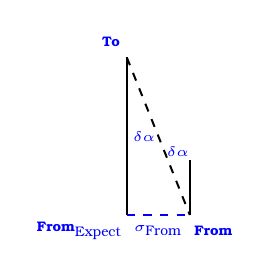
\begin{tikzpicture}
\draw (-0.2,2.2) node{{\color{blue}{\tiny{\textbf{To}}}}};
\draw (0.22,1) node{{\color{blue}{\tiny{$\delta \alpha$}}}};
\draw (0.65,0.8) node{{\color{blue}{\tiny{$\delta \alpha$}}}};
\draw[straight,color=black,line width=0.25mm] (0,2) -- (0,0);
\draw[straight,color=black,line width=0.25mm] (0.8,0) -- (0.8,0.7);
\draw[dashed,color=black,line width=0.25mm] (0,2) -- (0.8,0);
\draw[dashed,color=blue,line width=0.25mm] (0,0) -- (0.8,0);
\draw (-0.6,-0.2) node{{\color{blue}{\tiny{$\textbf{From}_{\text{Expect}}$}}}};
\draw (1.1,-0.2) node{{\color{blue}{\tiny{\textbf{From}}}}};
\draw (0.4,-0.2) node{{\color{blue}{\tiny{$\sigma_{\text{From}}$}}}};
\end{tikzpicture}~~~~~~~
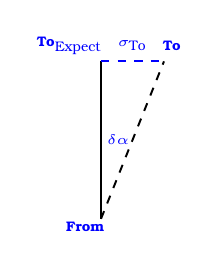
\begin{tikzpicture}
\draw (-0.2,-0.1) node{{\color{blue}{\tiny{\textbf{From}}}}};
\draw (0.22,1) node{{\color{blue}{\tiny{$\delta \alpha$}}}};
\draw[straight,color=black,line width=0.25mm] (0,0) -- (0,2);
\draw[dashed,color=black,line width=0.25mm] (0,0) -- (0.8,2);
\draw[dashed,color=blue,line width=0.25mm] (0,2) -- (0.8,2);
\draw (-0.4,2.2) node{{\color{blue}{\tiny{$\textbf{To}_{\text{Expect}}$}}}};
\draw (0.9,2.2) node{{\color{blue}{\tiny{\textbf{To}}}}};
\draw (0.4,2.2) node{{\color{blue}{\tiny{$\sigma_{\text{To}}$}}}};
\end{tikzpicture}
\caption{The ``From'' centering error is depicted on the left ($\tan\delta\alpha\approx\delta\alpha=\sigma_{\text{From}}/\text{D}_{\text{To,From}}$) and the ``To'' centering error is depicted on the right ($\tan\delta\alpha\approx\delta\alpha=\sigma_{\text{To}}/\text{D}_{\text{To,From}}$).  The expected azimuth is zero.}
\label{Fig:AZIM_Cent}
\end{figure}

\subsection{DGRP/HDIR: Horizontal Direction}
The error is the same as for AZIM records, where the ``From'' position is taken from the DGRP record and the ``To'' position is taken from the HDIR record.
\subsection{DIST: Distance Measurement}
The error applied to DIST measurement records due to Centering Errors and PPM takes the following form\footnote{We refer the reader to equation (7.38) of \cite{ghilani} for further details.}
\begin{equation}
\sigma_{\text{DIST,Centering\&PPM}}^2=(\sigma_{\text{From Centering Error}}*\cos(\alpha))^2+(\sigma_{\text{To Centering Error}}*\cos(\alpha))^2+\sigma_{\text{PPM}}^2\left(\f{\text{DIST}}{10^6\text{ m}}\right)^2.
\end{equation}
Where $\alpha$ is calculated as:

\begin{equation}
    \alpha=\arctan(\frac{\Delta U}{\sqrt{\Delta E^2 + \Delta N^2}})
\end{equation}

Where $\Delta E$, $\Delta N$, and $\Delta U$ are the component differences between the ``From'' and ``To'' points in the ENU reference frame.

\subsection{DXYZ: 3-D XYZ Coordinate Difference}
The error applied to DXYZ measurement records due to Centering Errors and PPM takes the following form
\begin{eqnarray}
&\textbf{Cov}_{\text{DXYZ,Centering\&PPM}}=\\\nonumber
&\textbf{Cov}_{\text{DXYZ,Centering}} + \textbf{Cov}_{\text{PPM}}
\end{eqnarray}

Where $\textbf{Cov}_{\text{PPM}}$ is defined as:

\begin{eqnarray}
    &\textbf{Cov}_{\text{DXYZ,PPM}}=\\\nonumber
    &\sigma_{\text{PPM}}^2\left(\f{\text{DIST}}{10^6\text{ m}}\right)^2\left(\begin{array}{ccc}1&0&0\\0&1&0\\0&0&1\end{array}\right).
\end{eqnarray}

The error applied to DXYZ measurement records due to centering errors is more complicated than for DIST records. First, define the error vector in the ENU frame:
\begin{equation}\label{eq:fctcENU} %\label{eq:ResCov}   
    \text{Fc/TcENU} = \left[ \begin{array}{ccc} \sigma_{\text{Fc/Tc}} & \sigma_{\text{Fc/Tc}} & 0 \\ \end{array} \right]
\end{equation}

Then, take the outer product of this vector with itself to get the measurement covariance in the ENU frame:
\begin{equation}\label{eq:fctcXYZ} %\label{eq:ResCov}   
    \textbf{Cov}_{\text{DXYZ,Fc/Tc,ENU}} =\left[ \begin{array}{c} \sigma_{\text{Fc/Tc}} \\ \sigma_{\text{Fc/Tc}} \\ 0 \\ \end{array} \right] \left[ \begin{array}{ccc} \sigma_{\text{Fc/Tc}} & \sigma_{\text{Fc/Tc}} & 0 \\ \end{array} \right] = \left[ \begin{array}{ccc} \sigma_{\text{Fc/Tc}}^2 & 0 & 0\\ 0 & \sigma_{\text{Fc/Tc}}^2 & 0\\ 0 & 0 & 0 \\ \end{array} \right]
\end{equation}

Then, rotate the result into the XYZ reference frame to get the final measurement covariance:

\begin{equation}\label{eq:dxyzCenterErr} %\label{eq:ResCov}   
    \textbf{Cov}_{\text{DXYZ,Fc/Tc,XYZ}} = \sigma_{\text{Fc/Tc}}^2 \text{R}_{ENU2XYZ} \left[ \begin{array}{ccc} 
                                                                                1 & 0 & 0 \\
                                                                                0 & 1 & 0 \\
                                                                                0 & 0 & 0 \\
                                                                            \end{array} \right] \text{R}_{ENU2XYZ}^{T}
\end{equation}


\subsection{HANG: Horizontal Angle}
The error applied to HANG measurement records due to Centering Errors takes the following form\footnote{We refer the reader to equations (7.9) and (7.21) of \cite{ghilani} for further details.}
\begin{eqnarray}
\sigma_{\text{HANG,Centering\&PPM}}^2=\left(\f{\sigma_{\text{From Centering Error}}}{\text{DIST}_{\text{From,At}}}\right)^2+\left(\f{\sigma_{\text{To Centering Error}}}{\text{DIST}_{\text{To,At}}}\right)^2&\\\nonumber
+\left(\f{\text{DIST}_{\text{To,From}}\hspace*{1mm}\sigma_{\text{At Centering Error}}}{\sqrt{2}\hspace*{1mm}\text{DIST}_{\text{From,At}}\hspace*{1mm}\text{DIST}_{\text{To,At}}}\right)^2.
\end{eqnarray}

\subsection{HDIF: Height Difference}
The error applied to HDIF measurement records due to PPM takes the following form
\begin{equation}
\sigma_{\text{HDIF,PPM}}^2=\sigma_{\text{PPM}}^2\left(\f{\text{DIST}}{10^6\text{ m}}\right)^2.
\end{equation}

\subsection{VANG: Vertical Angle}
The error applied to VANG measurement records due to Centering Errors takes the following form
\begin{eqnarray}
\sigma_{\text{VANG,Centering}}^2=\left(\f{\sin(\text{VANG}_{\text{To,From}})\sigma_{\text{From Centering Error}}}{\text{DIST}_{\text{To,From}}-\cos(\text{VANG}_{\text{To,From}})\sigma_{\text{From Centering Error}}}\right)^2&\\\nonumber
+\left(\f{\sin(\text{VANG}_{\text{To,From}})\sigma_{\text{To Centering Error}}}{\text{DIST}_{\text{To,From}}-\cos(\text{VANG}_{\text{To,From}})\sigma_{\text{To Centering Error}}}\right)^2.
\end{eqnarray}

This result may be found geometrically via Figure \ref{Fig:VANG_Cent}.
\begin{figure}[!htbp]
\centering
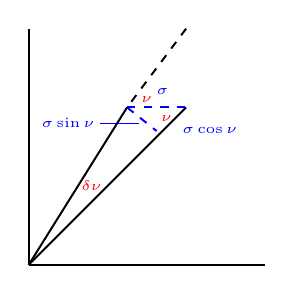
\begin{tikzpicture}
\draw[straight,color=black,line width=0.25mm] (0,0) -- (0,3);
\draw[straight,color=black,line width=0.25mm] (0,0) -- (3,0);
\draw[straight,color=black,line width=0.25mm] (0,0) -- (2,2);
\draw[straight,color=black,line width=0.25mm] (0,0) -- (1.25,2);
\draw[dashed,color=black,line width=0.25mm] (2,3) -- (1.25,2);
\draw[dashed,color=blue,line width=0.25mm] (1.25,2) -- (2,2);
\draw[dashed,color=blue,line width=0.25mm] (1.25,2) -- (1.625,1.7);
\draw[straight,color=blue,line width=0.15mm] (0.9,1.8) -- (1.4,1.8);
\draw (0.8,1) node{{\color{red}{\tiny{$\delta \nu$}}}};
\draw (1.7,2.2) node{{\color{blue}{\tiny{$\sigma$}}}};
\draw (2.3,1.7) node{{\color{blue}{\tiny{$\sigma\cos\nu$}}}};
\draw (0.5,1.8) node{{\color{blue}{\tiny{$\sigma\sin\nu$}}}};
\draw (1.75,1.857) node{{\color{red}{\tiny{$\nu$}}}};
\draw (1.5,2.1) node{{\color{red}{\tiny{$\nu$}}}};
\end{tikzpicture}
\caption{The geometry depicting the correction ($\tan\delta\nu\approx\delta\nu=\sigma\sin\nu/(\text{DIST}-\sigma\cos\nu)$).  The vertical angle is denoted by $\nu$ and the centering error by $\sigma$ in this diagram for brevity.  A similar argument holds for the ``From'' station.}
\label{Fig:VANG_Cent}
\end{figure}

\subsection{ZANG: Zenith Angle}
The error applied to ZANG measurement records due to Centering Errors takes the same form as for the VANG measurement records.
\section{Sigma}
The UNCR record provides the capability to add additional uncertainty to whichever measurement record type is of interest.  In particular, the Sigma field will always add to the variance such that
\begin{equation}
\sigma^2_{\text{Measurement Record,with additional}}=\sigma^2_{\text{Measurement Record}}+\sigma^2_{\text{additional}}.
\end{equation}
For the case of DXYZ records, the correction is of the form
\begin{equation}
\textbf{Cov}_{\text{DXYZ,with additional}}=\textbf{Cov}^2_{\text{Measurement Record}}+\sigma^2_{\text{additional}}\left(\begin{array}{ccc}1&0&0\\0&1&0\\0&0&1\end{array}\right).
\end{equation}
Note that this uncertainty contribution is accounted for prior to writing the *.dat file.



\chapter{Instrument Height Uncertainty Corrections}
\label{chap:InstrHghtCorrections}
Generally, in geodetic survey measurements, the instrument employed in a measurement isn't placed directly on the point being surveyed but is placed on a tripod which positions the instrument over the point at some convenient working height. The surveyor takes care to plumb the instrument over the point to minimize any lateral offsets and to measure the height offset that is introduced by the tripod. These actions (centering the instrument and measuring the height offset) typically cannot be achieved without some error. Centering errors, affecting the horizontal plane of the instrument, are handled by \textsf{salsa} through the UNCR (uncertainty) record as described in Chapter \ref{chap:UNCRcorrections}. The uncertainty in the measurement of an instrument height is the subject of this chapter.

For convenience, table \ref{tab:InstrHGHTcorrections} shows which measurments have ``To'' and ``From'' instrument heights as well as which measurements are affected by the uncertainty of the instrument height. Since instrument height uncertainties are a vertical correction, not every measurement type is affected even if it has a ``To'' or ``From'' height specified. In general, an instrument is placed at the ``From'' station and the target is at the ``To'' station. The one exception to this generality is the HANG measurement type, where the instrument is at the ``At'' station and the targets are at the ``To'' and ``From'' stations.
\begin{table}[!htbp]
\centering
\begin{tabular}{|l|c|c|c|c|c|c|c|c|}\hline
\tiny{\textbf{Record Type}}&\tiny{\textbf{Height From}}&\tiny{\textbf{Height To}}&\tiny{\textbf{Height Uncertainty}}\\\hline
\tiny{\textbf{AZIM}}&\tiny{\textbf{X}}&\tiny{\textbf{X}}&\\\hline
\tiny{\textbf{DGRP}}&&&\\\hline
\tiny{\textbf{DIST}}&\tiny{\textbf{X}}&\tiny{\textbf{X}}&\tiny{\textbf{X}}\\\hline
\tiny{\textbf{DXYZ}}&\tiny{\textbf{X}}&\tiny{\textbf{X}}&\tiny{\textbf{X}}\\\hline
\tiny{\textbf{HANG}}&\tiny{\textbf{X}}&\tiny{\textbf{X}}&\\\hline
\tiny{\textbf{HDIF}}&&&\\\hline
\tiny{\textbf{VANG}}&\tiny{\textbf{X}}&\tiny{\textbf{X}}&\tiny{\textbf{X}}\\\hline
\tiny{\textbf{ZANG}}&\tiny{\textbf{X}}&\tiny{\textbf{X}}&\tiny{\textbf{X}}\\\hline
\end{tabular}
\caption{Table indicating which instrument height uncertainties are applicable to each record type.}
\label{tab:InstrHGHTcorrections}
\end{table}
\section{Instrument Height Uncertainties}
Note that instrument height uncertainties in \textsf{salsa} are treated as vertical errors. In summary, only these four measurment types are affected: DIST, DXYZ, VANG and ZANG.

\subsection{DIST: Distance Measurement}
The error applied to DIST measurement records due to instrument height uncertainty takes the following form:
\begin{equation}
\sigma_{\text{DIST,Instr HGHT}}^2=(\sigma_{\text{Height From}}\sin(\alpha))^2+(\sigma_{\text{Height To}}\sin(\alpha))^2.
\end{equation}

Where $\alpha$ is calculated the same as in chapter \ref{chap:UNCRcorrections}. The expression for $\alpha$ is repeated here for convenience:

\begin{equation}
    \alpha=\arctan(\frac{| \Delta U |}{\sqrt{\Delta E^2 + \Delta N^2}})
\end{equation}

Where $\Delta E$, $\Delta N$, and $\Delta U$ are the component differences between the ``From'' and ``To'' points in the ENU reference frame.

\subsection{DXYZ: 3-D XYZ Coordinate Difference}
The error applied to DXYZ measurement records due to instrument height uncertainty is more complicated than for DIST records. First, define the error vector in the ENU frame:
\begin{equation}\label{eq:heightENU} %\label{eq:ResCov}   
    \text{HeightFrom/ToENU} = \left[ \begin{array}{ccc} 0 & 0 & \sigma_{\text{Height From/To}} \\ \end{array} \right]
\end{equation}

Then, take the outer product of this vector with itself to get the measurement covariance in the ENU frame:
\begin{equation}\label{eq:heightXYZ} %\label{eq:ResCov}   
    \text{Cov}_{\text{DXYZ,Instr HGHT,ENU}} =\left[ \begin{array}{c} 0 \\ 0 \\ \sigma_{\text{H}} \\ \end{array} \right] \left[ \begin{array}{ccc} 0 & 0 & \sigma_{\text{H}} \\ \end{array} \right] = \left[ \begin{array}{ccc} 0 & 0 & 0\\ 0 & 0 & 0\\ 0 & 0 & \sigma_{\text{H}}^2 \\ \end{array} \right]
\end{equation}

The, rotate the result into the XYZ reference frame:

\begin{equation}\label{eq:dxyzHeightErr} %\label{eq:ResCov}   
    \text{Cov}_{\text{DXYZ,Instr HGHT, XYZ}} = \sigma_{\text{H}}^2 \text{R}_{ENU2XYZ} \left[ \begin{array}{ccc} 
                                                                                0 & 0 & 0 \\
                                                                                0 & 0 & 0 \\
                                                                                0 & 0 & 1 \\
                                                                            \end{array} \right] \text{R}_{ENU2XYZ}^{T}
\end{equation}

The total measurement covariance for both the ``From'' and ``To'' stations is:

\begin{equation}\label{eq:totalDXYZHeightCov} %\label{eq:ResCov}   
    \text{Cov}_{\text{DXYZ,Instr HGHT Total},XYZ} = \text{Cov}_{\text{DXYZ,Instr HGHT From},XYZ} + \text{Cov}_{\text{DXYZ,Instr HGHT To},XYZ}
\end{equation}

Where the measurement covariances for each station are defined by \ref{eq:dxyzHeightErr}.

\subsection{VANG: Vertical Angle}
The error applied to VANG measurement records due to instrument height uncertainty takes the following form where $\text{S}$ is the slant distance, $\text{d}$ is the horizontal distance between the two points, and $\text{H}$ is the vertical distance between the two points:
\begin{eqnarray}\label{eq:varianceVANG}
\sigma_{\text{VANG,Instr HGHT}}^2=\left(\f{\f{H}{\text{S}} - \f{H-\sigma_{H_{From}}}{\sqrt{d^2 + (H-\sigma_{H_{From}})^2}}}{\cos(\text{VANG}_{\text{To,From}})}\right)^2&\\\nonumber
+\left(\f{\f{H}{\text{S}} - \f{H-\sigma_{H_{To}}}{\sqrt{d^2 + (H-\sigma_{H_{To}})^2}}}{\cos(\text{VANG}_{\text{To,From}})}\right)^2
\end{eqnarray}

This result may be found geometrically via figure \ref{Fig:VANG_instr_hght}.
\begin{figure}[!htbp]
\centering
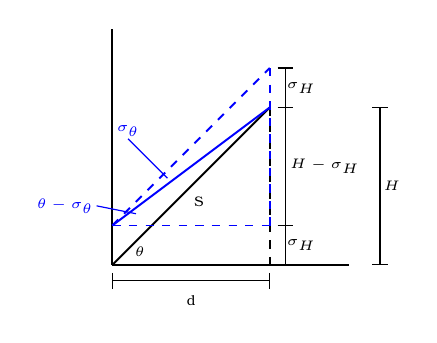
\begin{tikzpicture}
\draw[straight,color=black,line width=0.25mm] (0,0) -- (0,3);
\draw[straight,color=black,line width=0.25mm] (0,0) -- (3,0);
\draw[straight,color=black,line width=0.25mm] (0,0) -- (3,0);
\draw[straight,color=black,line width=0.25mm] (0,0) -- (2,2);
\draw[straight,color=blue,line width=0.25mm] (0,0.5) -- (2,2);
\draw[dashed,color=blue,line width=0.25mm] (0,0.5) -- (2,2.5);

\draw[dashed,color=black,line width=0.25mm] (2,2) -- (2,0);
\draw[dashed,color=blue,line width=0.25mm] (2,2.5) -- (2,0.5);
\draw[dashed,color=blue,line width=0.25mm] (0,0.5) -- (2,0.5);
\draw[dashed,color=blue,line width=0.25mm] (0,0.5) -- (2,0.5);



\draw[straight,color=blue,line width=0.15mm] (0.2,1.6) -- (0.7,1.1);
\draw[straight,color=blue,line width=0.15mm] (-0.2,0.75) -- (0.3,0.65);

\draw (1,-0.45) node{{\color{black}{\tiny{$\text{d}$}}}};
\draw (1.1,0.8) node{{\color{black}{\tiny{$\text{S}$}}}};


\draw (0.35,0.17) node{{\color{black}{\tiny{$\theta$}}}};
\draw (-0.6,0.75) node{{\color{blue}{\tiny{$\theta - \sigma_{\theta}$}}}};
\draw (0.2,1.7) node{{\color{blue}{\tiny{$\sigma_{\theta}$}}}};

\draw (2.4,0.25) node{{\color{black}{\tiny{$\sigma_{H}$}}}};
\draw (2.7,1.25) node{{\color{black}{\tiny{$H - \sigma_{H}$}}}};
\draw (2.4,2.25) node{{\color{black}{\tiny{$\sigma_{H}$}}}};
\draw (3.55,1) node{{\color{black}{\tiny{$H$}}}};

\draw[straight,color=black,line width=0.15mm] (0, -0.1) -- (0, -0.3);
\draw[straight,color=black,line width=0.15mm] (2, -0.1) -- (2, -0.3);
\draw[straight,color=black,line width=0.15mm] (0, -0.2) -- (2, -0.2);


\draw[straight,color=black,line width=0.15mm] (2.1,0.5) -- (2.3,0.5);
\draw[straight,color=black,line width=0.15mm] (2.1,2) -- (2.3,2);
\draw[straight,color=black,line width=0.15mm] (2.1,2.5) -- (2.3,2.5);
\draw[straight,color=black,line width=0.15mm] (2.2,0) -- (2.2,2.5);

\draw[straight,color=black,line width=0.15mm] (3.3,0) -- (3.5,0);
\draw[straight,color=black,line width=0.15mm] (3.3,2) -- (3.5,2);
\draw[straight,color=black,line width=0.15mm] (3.4,0) -- (3.4,2);
\end{tikzpicture}
\caption{The geometry depicting the effect of instrument height uncertainty at the ``From'' station, $\sigma_{H_{from}}$, on the measured Vangle, $\theta$.  A similar argument holds for the ``To'' station.}
\label{Fig:VANG_instr_hght}
\end{figure}

From this diagram one can derive the previously given equation for the measurement variance. First, establish some basic identities:

\begin{equation}\label{eq:sin} %\label{eq:ResCov}   
    \sin\theta = \f{H}{S}; \sin\left(\theta-\sigma_{\theta_{From}}\right) = \f{H-\sigma_{H_{From}}}{S*}
\end{equation}

Where:
\begin{equation}\label{eq:s_sPrime} %\label{eq:ResCov}   
    S = \sqrt{d^2 + H^2}; S* = \sqrt{d^2 + (H-\sigma_{H_{From}})^2}
\end{equation}

Next using basic trigonometric identities:
\begin{equation}\label{eq:sin_start} %\label{eq:ResCov} 
    \sin\left(\theta-\sigma_{\theta_{From}}\right) = \f{H-\sigma_{H_{From}}}{S*}
\end{equation}
\begin{equation}
    \sin\theta\cos\sigma_{\theta_{From}} - \cos\theta\sin\sigma_{\theta_{From}} = \f{H-\sigma_{H_{From}}}{S*}
\end{equation}

And following the small angle assumption:
\begin{equation}\label{eq:small_angle_assumption} %\label{eq:ResCov} 
    \sin\theta - \cos\theta\sigma_{\theta_{From}} = \f{H-\sigma_{H_{From}}}{S*}
\end{equation}
\begin{equation}
    \f{H}{S} - \cos\theta\sigma_{\theta_{From}} = \f{H-\sigma_{H_{From}}}{S*}
\end{equation}
\begin{equation}
    \cos\theta\sigma_{\theta_{From}} = \f{H}{S} - \f{H-\sigma_{H_{From}}}{S*}
\end{equation}
\begin{equation}
    \sigma_{\theta_{From}} = \f{\f{H}{S}- \f{H-\sigma_{H_{From}}}{S*}}{\cos\theta}
\end{equation}

The derivation for $\sigma_{\theta_{To}}$ is analagous. Therefore, to achieve the variance equation \ref{eq:varianceVANG}, square both the ``From'' and ``To'' results and add them together.


\subsection{ZANG: Zenith Angle}
The error applied to ZANG measurement records due to instrument height uncertainty takes the same form as for the VANG measurement records. The only difference is $\cos$ becomes $\sin$.



\chapter{Station Inverse Data}
\label{chap:StatInvDat}

The Station Inverse dialog box is primarily intended to provide the user with various metrics that relate the states of two user-selected stations.  Many of these relative quantities have been defined previously: the azimuth angle in section \ref{subsection:AZIM}, the slant distance in section \ref{subsection:DIST}, the 3-D XYZ vector in section \ref{subsection:DXYZ}, the height difference in section \ref{subsection:HDIF}, and the vertical angle in section \ref{subsection:VANG}.  Note that the Station Inverse dialog box only functions after an adjustment has been run (including the calculation of any derived points), as the values within the Station Inverse dialog box require the h5 file generated by the adjustment process.  

\section{Station Inverse Dialog Data Generation}
The Station Data Dialog box shown in Figure \ref{fig:StationInverseDialog} provides a user interface through which the user can add and remove station inverse pairs. Individual information for each station is provided in the left half of the dialog box. Relative information between stations is provided in the right half of the dialog box. The center table serves as a graphical display of the station inverse pairs that will have their metrics generated in \verb+<Project Name>.inv+ and \verb+<Project Name>Inv.csv+ files. The following subsections detail the various actions the user can perform in the Station Data Dialog box and the steps that are executed to generate the output inverse pair data.

\begin{figure} [!htb]
	\centering
	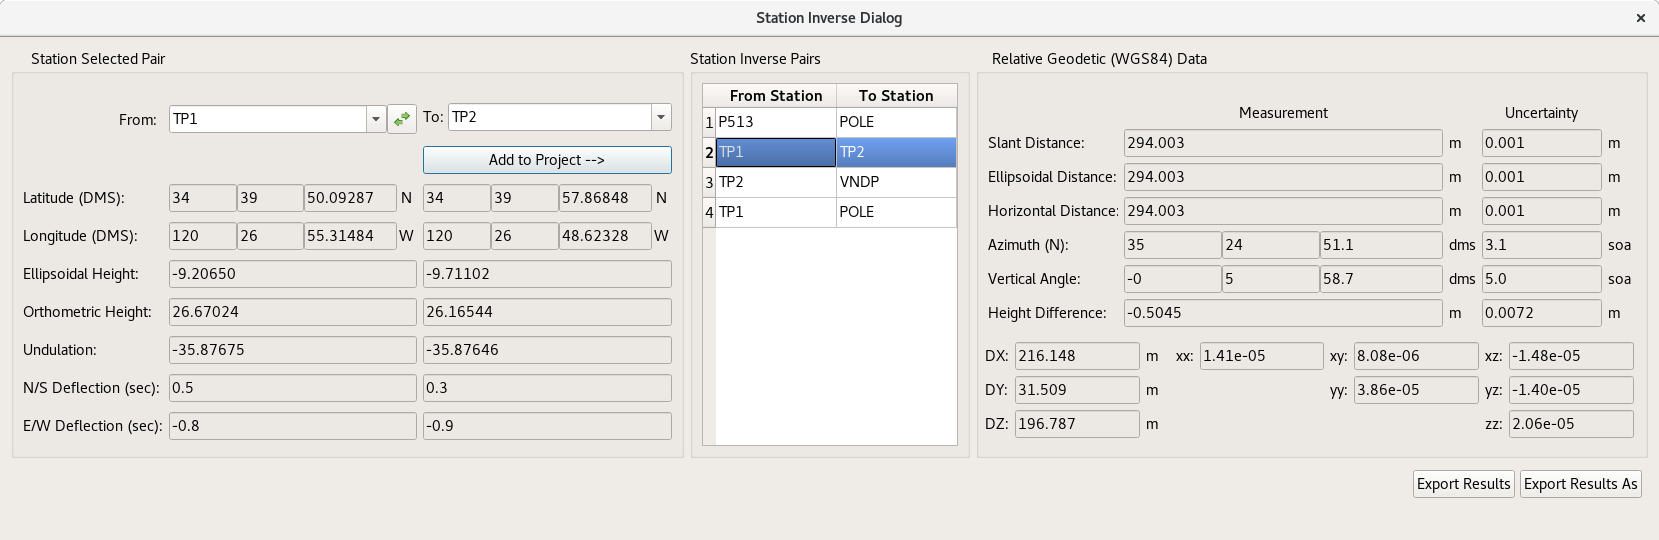
\includegraphics[trim = 0mm 0mm 0mm 0mm, clip, width=1.0\textwidth]{StationInverseDialog.png} % or linewidth
	% Trim option parameter order: left bottom right top
	\caption{Station Inverse Dialog}
	\label{fig:StationInverseDialog}
\end{figure}

\subsection{Interacting with the Station Data Dialog Interface} \label{sect:SDDInter}
Upon selecting View $\ra$ Station Inverse from the main window, the Station Data Dialog box table will be loaded with all prior existing pairs. For more information regarding the parsing of the \verb+<Project Name>Inverses.cfg+ file refer to the appendix "Inverse Configuration Parsing". This interface allows the user to perform the following actions.

\begin{itemize}
	\item \emph{Add Pair to Project} - Comboboxes allow the user to user to select stations that were enabled for the last adjustment. Once a station has been selected in the To and From comboboxes they may be added to the list by clicking the Add to Project button. Note that if a station pair already exists in the list or if the To and From comboboxes have the same value, then the pair will not be added to the list.
	\item \emph{Remove Pair(s) from Project} - Left clicking a row will highlight an individual pair. Additional pairs can be highlighted individually by pressing Shift and Click on the other desired row. Additionally, once a row is selected the user can hit Ctrl + Shift + Click to highlight everything between the original row and the newly selected row. Once the desired row(s) are highlighted they may be removed by pressing Right Click and selecting Delete or by pressing the Delete key.
	\item \emph{Export Results} - Upon clicking the Export Results button all of the valid pairs in the center table will have their data generated to an output file. For more information please refer to section \ref{sect:InverseGen}
	\item \emph{Export Results As} - Behaves in a similar manner to \emph{Export Results} but with extended functionality. This button will bring up a file dialog box where the user can select the output directory to save their inv and csv files and input a new base name for the output files as well. This button should be utilized if it is not desired that the output be placed in the project directory or an output file convention differing from the default \verb+<Project Name>.inv+ and \verb+<Project Name>Inv.csv+ is desired. This allows the user to backup the current results of the inverse calculations such that they will not be overwritten (as \verb+<Project Name>.inv+ and \verb+<Project Name>Inv.csv+ will be) by subsequent modifications and adjustments to the project.
	\item \emph{Pair Selection} - Highlighting an individual pair by clicking its row, or selecting an up or down arrow will update the text boxes to display the metrics for that station inverse pair. If the pair is invalid, the boxes will be cleared.
\end{itemize}

\subsection{Inverse Pair Data Generation} \label{sect:InverseGen}
Upon clicking one of the Export buttons from the Station Data Dialog box or selecting Project $\ra$ Calculate Adjustment from the main Salsa interface the following sequence will be executed.

\begin{enumerate}
	\item Project will search for \verb+<Project Name>Inverses.cfg+ file. If not found an early exit will occur.
	\item The file will be parsed for all unique, valid pairs. A pair is considered valid if
	\begin{itemize}
		\item The From and To stations have labels that correspond to an existing POSG, POSC or derived point record.
		\item Both stations were enabled at the time Calculate Adjustment was last performed.
		\item The pair is non-trivial, i.e. the From and To stations do not have the same label. 
	\end{itemize}
	\item Output \verb+<Project Name>.inv+ and \verb+<Project Name>Inv.csv+ files will be generated containing the metrics for valid inverse pairs.
\end{enumerate}

The inv output file is a plain text file which writes each quantity from the Station Data Dialog GUI on its own line. It is meant to serve as a human readable format for all of the station inverse pairs. Conversely, the csv file delimits quantities using commas and has only one line per station pair. 

\section{Station Inverse Dialog Relative Geodetic (WGS84) Data Definitions}

As described above, all relative quantities between the two provided stations are defined in sections \ref{subsection:AZIM} through \ref{subsection:VANG}, with the exception of the ellipsoidal distance and the horizontal distance.  For these quantities previously defined, the corresponding uncertainties are also computed via the equivalent measurement first order partial derivative matrices that are employed in an adjustment.  These uncertainties are displayed within the Station Inverse dialog box next to the nominal values.  All quantities are specified in meters, except for the azimuth and vertical angles between the stations which are provided in degrees, minutes, and seconds of arc, along with the associated uncertainties in seconds of arc.  Also note that the DXYZ vector covariance is provided, which includes both the diagonal and off-diagonal covariance values. 

The ellipsoidal distance is the shortest distance along the surface of the WGS 84 ellipsoid from the ``From'' station latitude and longitude to the ``To'' station latitude and longitude.  The horizontal distance is the magnitude of the relative station vector projected into the horizontal plane, which is defined using the East-North-Up frame computed at the ``From'' station.  The ellipsoidal distance and the horizontal distance between a ``From'' and ``To'' station are shown in Figure \ref{fig:RelativeStationDistances}, along with the previously defined slant distance (section \ref{subsection:DIST}).
\begin{figure} [!htb]
	\centering
	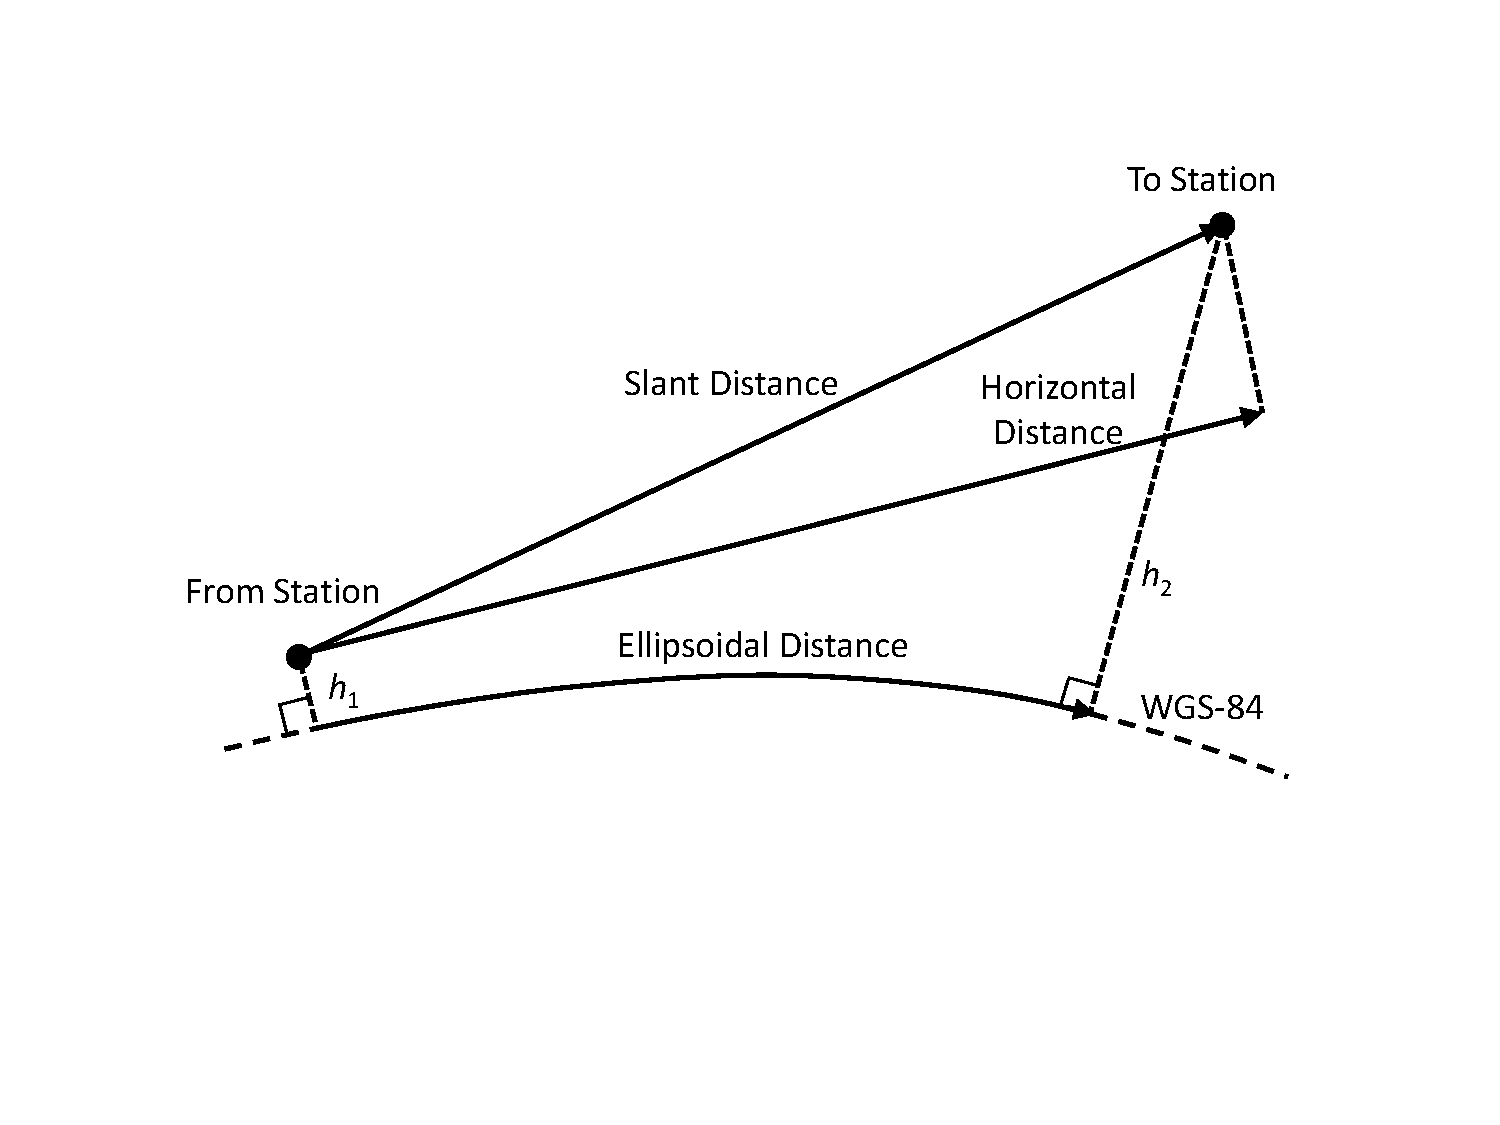
\includegraphics[trim = 30mm 55mm 35mm 25mm, clip, width=1.0\textwidth]{DistanceDiagramV2.pdf} % or linewidth
	% Trim option parameter order: left bottom right top
	\caption{Relative Station Distances}
	\label{fig:RelativeStationDistances}
\end{figure}


\subsection{Ellipsoidal Distance}

The Ellipsoidal distance is in general defined as the shortest distance along the surface of a three dimensional ellipsoid between two points on the ellipsoid.  The ellipsoid used in SALSA is  WGS 84, which is an ellipsoid of revolution with a flattening parameter $f = 1/298.257223563$ and semi-major axis (SMA) $a_{WGS84} = 6378137.0$ meters.  The two points on the surface are often defined using their geodetic latitude and longitude values.

\subsubsection{Vincenty's Method for Ellipsoidal Distance Computation} \label{sect:Vincenty}

To compute the ellipsoidal distance between the ``From'' and ``To'' station locations, the commonly used Vincenty's Method is employed \cite{vincenty1975direct}. Vincenty's Method is an iterative numerical approach that provides consistent geodesic distance values between all points on an ellipsoid, except those points antipodal (i.e. on exactly opposite sides of the Earth) to each other (or nearly antipodal).

The semi-minor axis is needed for Vincentys method, and is computed as
\begin{equation}
b = (1 - f)a
\end{equation}

The geodesic latitude $\phi$ and longitude $\lambda$ for the two stations are assumed to be known, and the longitude difference is computed as 
\begin{equation}
\Delta\lambda = \lambda_2 - \lambda_1
\end{equation}
where $\lambda_2$ represents the longitude of the ``To'' station, and $\lambda_1$ represents the longitude of the ``From'' station.  These subscripts will be used for these stations for the remainder of this derivation.  The ``reduced latitude'' of each station (i.e. the latitude on the auxiliary sphere) is computed as
\begin{equation}
\begin{split}
U_1 &= \tan^{-1}\left[ (1-f) \tan(\phi_1) \right] \\ 
U_2 &= \tan^{-1}\left[ (1-f) \tan(\phi_2) \right]
\end{split}
\end{equation}

The quantity $\bar{\lambda}$ is initialized as the longitude difference:
\begin{equation}
\bar{\lambda} = \Delta\lambda
\end{equation}
The following equations are then iterated upon until $\bar{\lambda}$ converges (as dictated by a change in magnitude $||\Delta\bar{\lambda}||$ of less than $1 \times 10^{-12}$):
\begin{equation}
\sin \sigma = \sqrt{(\cos U_2\sin \bar{\lambda})^2 + (\cos U_1 \sin U_2 - \sin U_1 \cos U_2 \cos \bar{\lambda} )^2}
\end{equation}
\begin{equation}
\cos \sigma = \sin U_1 \sin U_2 + \cos U_1 \cos U_2 \cos \bar{\lambda}
\end{equation}
\begin{equation}
\sigma = \tan^{-1} \frac{\sin \sigma}{\cos \sigma}
\end{equation}
\begin{equation}
\sin \alpha = \frac{\cos U_1 \cos U_2 \sin \bar{\lambda}}{\sin \sigma}
\end{equation}
\begin{equation}
\cos^2 \alpha = 1 - \sin^2 \alpha
\end{equation}
\begin{equation}
\cos(2 \sigma_m) = \cos \sigma - \frac{2 \sin U_1 \sin U_2}{\cos^2 \alpha}
\end{equation}
\begin{equation}
C = \frac{f}{16} \cos^2 \alpha \left[ 4 + f \left(4 - 3 \cos^2 \alpha \right) \right]
\end{equation}
\begin{equation}
\begin{split}
\bar{\lambda}_{\text{new}} =& \Delta\lambda + (1 - C) f \sin \alpha \\ 
& * \left\lbrace \sigma + C \sin \sigma \left[ \cos(2\sigma_m) + C \cos\sigma \left(-1 + 2 \cos^2(2\sigma_m) \right) \right]  \right\rbrace 
\end{split}
\end{equation}
\begin{equation}
\Delta\bar{\lambda} = \bar{\lambda}_{\text{new}} - \bar{\lambda}_{\text{prev}}
\end{equation}

After $\bar{\lambda}$ has converged, the ellipsoidal distance $s$ is computed using equations:
\begin{equation}
u^2 = \cos^2 \alpha \frac{a^2 - b^2}{b^2}
\end{equation}
\begin{equation}
k_1 = \frac{\sqrt{1 + u^2} - 1}{\sqrt{1 + u^2} + 1} 
\end{equation}
\begin{equation}
A = \frac{1 + \tfrac{1}{4} k_1^2}{1-k_1}
\end{equation}
\begin{equation}
 B = k_1 \left(1 - \tfrac{3}{8} k_1^2 \right)
\end{equation}
\begin{equation}
\begin{split}
\Delta\sigma =& B \sin\sigma \left\lbrace \cos(2 \sigma_m) + \tfrac{1}{4} B \left[ \cos\sigma \left(-1 + 2 \cos^2(2\sigma_m) \right) \right. \right. \\
& \left. \left. - \tfrac{1}{6} B \cos(2\sigma_m) (-3 + 4 \sin^2\sigma) (-3 + 4 * \cos^2(2\sigma_m)) \right] \right\rbrace
\end{split}
\end{equation}
\begin{equation}
s = b A (\sigma - \Delta\sigma)
\end{equation}

For two points that are exactly on the equator (i.e. the geodetic latitude is zero), the value for the $\cos(2 \sigma_m)$ term is set to zero to avoid a singularity in the computation of that parameter (the term is not not used anyways when both points are exactly on the equator).  

\subsubsection{Sigma Point Transform for Uncertainty Mapping}

The unscaled sigma point transform \cite{julier1995new} is employed to map the uncertainty in both station positions into a single uncertainty value for the ellipsoidal distance. Compared to the standard linearized approach of pre- and post-multiplying the solution covariance by first order partial derivative matrices, the sigma point transform better captures the performance of nonlinear functions, while eliminating the need to compute the partial derivative matrices.

The two station positions in ECEF XYZ coordinates are stacked into a single vector as
\begin{equation}
\boldsymbol{x} = \left[ \begin{array}{c} 
\boldsymbol{r}_{\text{From}} \\ \boldsymbol{r}_{\text{To}}
\end{array} \right]
\end{equation}

The ECEF XYZ covariance of both stations is $\text{Cov}_x$, which includes cross covariance terms between the stations. To obtain $\text{Cov}_x$, the covariance values associated with these two stations are extracted from the total covariance matrix:
\begin{equation}
\text{Cov}_x = \left[ \begin{array}{cc} 
\text{Cov}_{\text{From}} & \text{Cov}_{\text{FromCrossTo}} \\ \text{Cov}_{\text{FromCrossTo}}^T & \text{Cov}_{\text{To}}
\end{array} \right]
\end{equation}



The Cholesky decomposition \cite{golub1996matrix} of $\text{Cov}_x$ is computed:
\begin{equation}
\rtc{\text{Cov}_x} = \text{chol}\left( \text{Cov}_x \right)
\end{equation}
where
\begin{equation} \label{eq:chol_decomp}
\text{Cov}_x = \rtc{\text{Cov}_x} \rtc{\text{Cov}_x}^T
\end{equation}

The Cholesky decomposition matrix is notionally considered the ``square root'' of the covariance matrix.  However, the covariance when working with derived points can often be positive semi-definite instead of positive definite: some of the eigenvalues of the matrix are zero as a result of having one or more position components fixed.  The Cholesky decomposition process requires a positive definite matrix input in order to provide a unique solution. Fortunately, the Cholesky decomposition process is stable as the eigenvalues of a matrix approach zero (i.e. changing the eigenvalue from one very small value to another very small value does significantly not change the decomposition), and thus small values can be substituted for any zero-value eigenvalues to obtain a Cholesky decomposition that is correct to any desired precision \cite{wiki:Cholesky,fang2008modified}.

To determine if there are any zero-value eigenvalues before performing the Cholesky decomposition, the eigenvalues and associated eigenvectors for the $\text{Cov}_x$ matrix are computed via the EigenSolver tool within the Eigen library \cite{EigenSolver}:
\begin{equation} \label{eq:eigDecomp}
\text{Cov}_x = U \Lambda U^T
\end{equation}
where $\Lambda$ is a diagonal matrix with eigenvalues on the diagonal, and $U$ is an orthogonal matrix consisting of the eigenvectors associated with the eigenvalues in $\Lambda$.  If any eigenvalues are zero or slightly negative (likely resulting from numerical precision limitations), these values are changed to a very small positive value $\epsilon$.  After this change, the covariance matrix can be reassembled via equation \ref{eq:eigDecomp}.  Then the Cholesky decomposition can be executed to obtain the ``square root'' covariance matrix described in equation \ref{eq:chol_decomp}.  

The covariance square root matrix is then employed to deterministically generate a set of vectors called ``sigma point vectors'':
\begin{equation}
\begin{split}
\mathcal{X} = \left[ \right. & x + \sqrt{n} \rtc{\text{Cov}_x}(:,1),x + \sqrt{n} \rtc{\text{Cov}_x}(:,2), ... ,  \\
                   & \left.x - \sqrt{n} \rtc{\text{Cov}_x}(:,1),x - \sqrt{n} \rtc{\text{Cov}_x}(:,2), ... \right]
\end{split}
\end{equation}
where $n$ is the number of dimensions of the initial vector (six in this two-station example), and the notation $(:,i)$ indicates the $i^{\text{th}}$ column of the $\rtc{\text{Cov}_x}$ matrix. Each column of $\mathcal{X}$ represents a sigma point vector, also described as $\mathcal{X}_i$ for column $i$. 

These sigma point vectors can be used to map the formal covariance of the station positions to the uncertainty in the ellipsoidal distance. Each sigma point vector $\mathcal{X}_i$ is mapped through the nonlinear function $g(x,a,f)$ which includes the conversion from Cartesian ECEF XYZ positions of both stations to geodetic coordinates and applying Vincenty's Method (section \ref{sect:Vincenty}) to compute the ellipsoidal distance:
\begin{equation}
\mathcal{Y}_i = g(\mathcal{X}_i,a,f)
\end{equation}

The mean of the mapped sigma points, which does not necessarily equal the computed ellipsoidal distance using the nominal station positions, is
\begin{equation}
\hat{y} = \frac{1}{2n} \sum_{i=1}^{2n} \mathcal{Y}_i
\end{equation}
The mean and mapped sigma point vectors are used to compute the mapped covariance matrix:
\begin{equation}
\text{Cov}_y = \frac{1}{2n} \sum_{i=1}^{2n} \left(\mathcal{Y}_i - \hat{y}\right) \left(\mathcal{Y}_i - \hat{y}\right)^T
\end{equation}
Note that the dimension of $\hat{y}$ and $\text{Cov}_y$ will be $1$ and $1 \times 1$ for the single geodesic distance output, and thus
\begin{equation}
\sigma_{\text{ellipsoidal}} = \sqrt{\text{Cov}_y}
\end{equation}

% Removing to avoid confusion
% \textbf{Note}: The scaling of the ellipsoid is not included in the sigma point transform, under the assumption it is desired to have a constant ellipsoid based on the nominal ``From'' station position, and not a new ellipsoid for each sigma point.  Additionally, performing this adjustment for each sigma point is not likely to make a significant difference on the mapped uncertainty, while introducing more computation required for each sigma point transformation.


\subsection{Horizontal Distance}

The horizontal distance between two stations is defined as the magnitude of the 2D vector between the stations that results from projecting the relative 3D vector into the horizontal plane.  Given the two station positions in ECEF cartesian frame coordinates, the relative station vector is
\begin{equation} \label{eq:RelVect}
\boldsymbol{r}_{\text{rel}}^{\text{XYZ}} = \boldsymbol{r}_{\text{To}} - \boldsymbol{r}_{\text{From}}
\end{equation}
This $\boldsymbol{r}_{\text{rel}}^{\text{XYZ}}$ vector is projected into the horizontal plane, defined as perpendicular to the WGS 84 ellipsoid at the ``from'' station coordinates:
\begin{equation}
\boldsymbol{r}_{\text{rel}}^{\text{ENU}} = R_{\text{XYZ}}^{\text{ENU}} \boldsymbol{r}_{\text{rel}}^{\text{XYZ}}
\end{equation}
where $R_{\text{XYZ}}^{\text{ENU}}$ is the rotation matrix from the ECEF frame to the ENU frame (which is also fixed to the surface of the Earth). The $R_{\text{XYZ}}^{\text{ENU}}$ rotation matrix is defined as:
\begin{equation}
R_{\text{XYZ}}^{\text{ENU}} = \left[ \hat{E} \: \hat{N} \; \hat{U} \right]^T
\end{equation}
where the unit vectors $\hat{E}$, $\hat{N}$, and $\hat{U}$ are the unit vectors of the east, north, and up directions in the ECEF frame at the ``From'' station. The terms of $R_{\text{XYZ}}^{\text{ENU}}$ are defined in equation \ref{eq:ECEF2ENU}. 

To obtain the horizontal distance, the RSS magnitude of the east and north components is computed:
\begin{equation} \label{eq:HorizontalDist}
D_{\text{horizontal}} = \sqrt{\boldsymbol{r}_{\text{rel}}^{\text{ENU}}(1)^2 + \boldsymbol{r}_{\text{rel}}^{\text{ENU}}(2)^2}
\end{equation}

To determine the uncertainty in the horizontal distance, the same unscaled sigma point transform is employed as described above for the ellipsoidal distance. The mapping function is the horizontal distance calculation provided in equations \ref{eq:RelVect} through \ref{eq:HorizontalDist} instead of the ellipsoidal distance, but otherwise the approach is identical.


\chapter{Custom Import and Export Scripts}
\label{chap:customImportExport}

SALSA supports the importing of instrument files into a project through Import menu actions.  Furthermore, various output formats are available through Export menu actions.  Selecting these menu actions causes SALSA to initiate a python script which has been bundled with SALSA.  This section will explain how the user may write their own custom import and export scripts which populate these menus.

\section{Discoverable Scripts}\label{sec:discoverableScripts}

SALSA will auto-populate the Import and Export menus with scripts which are located in special folders within the project directory.  The scripts which the user would like to populate the Import menu should be placed within a customImport folder within the project directory.  The scripts which the user would like to populate the Export menu should be placed within a customExport folder within the project directory.  In Figure \ref{Fig:customImportExport} we demonstrate a typical file structure.

\begin{figure}[!htbp]
\centering
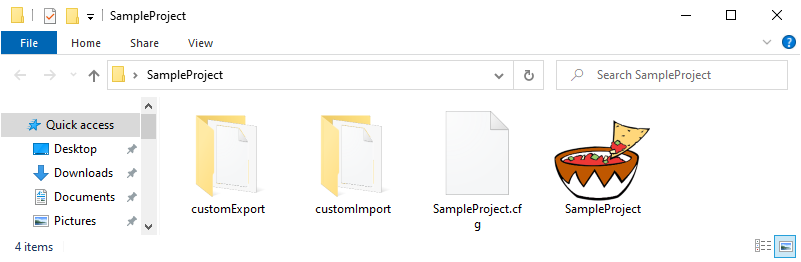
\includegraphics[width=1\textwidth]{customImportExport_fileStructure.png}\\
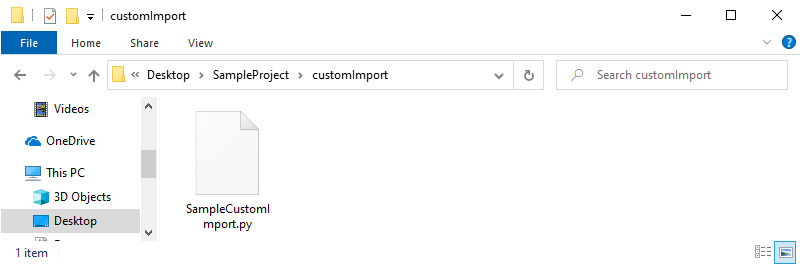
\includegraphics[width=1\textwidth]{customImport_fileStructure.png}\\
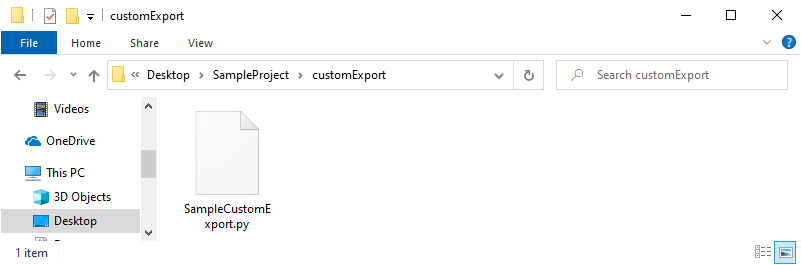
\includegraphics[width=1\textwidth]{customExport_fileStructure.png}
\caption{To be discoverable by SALSA, custom import scripts must be placed in the customImport folder and custom export scripts must be placed in the customExport folder.}
\label{Fig:customImportExport}
\end{figure}

The custom scripts populate SALSA in the manner depicted in Figure \ref{Fig:customImportExportGUI}.

\begin{figure}[!htbp]
\centering
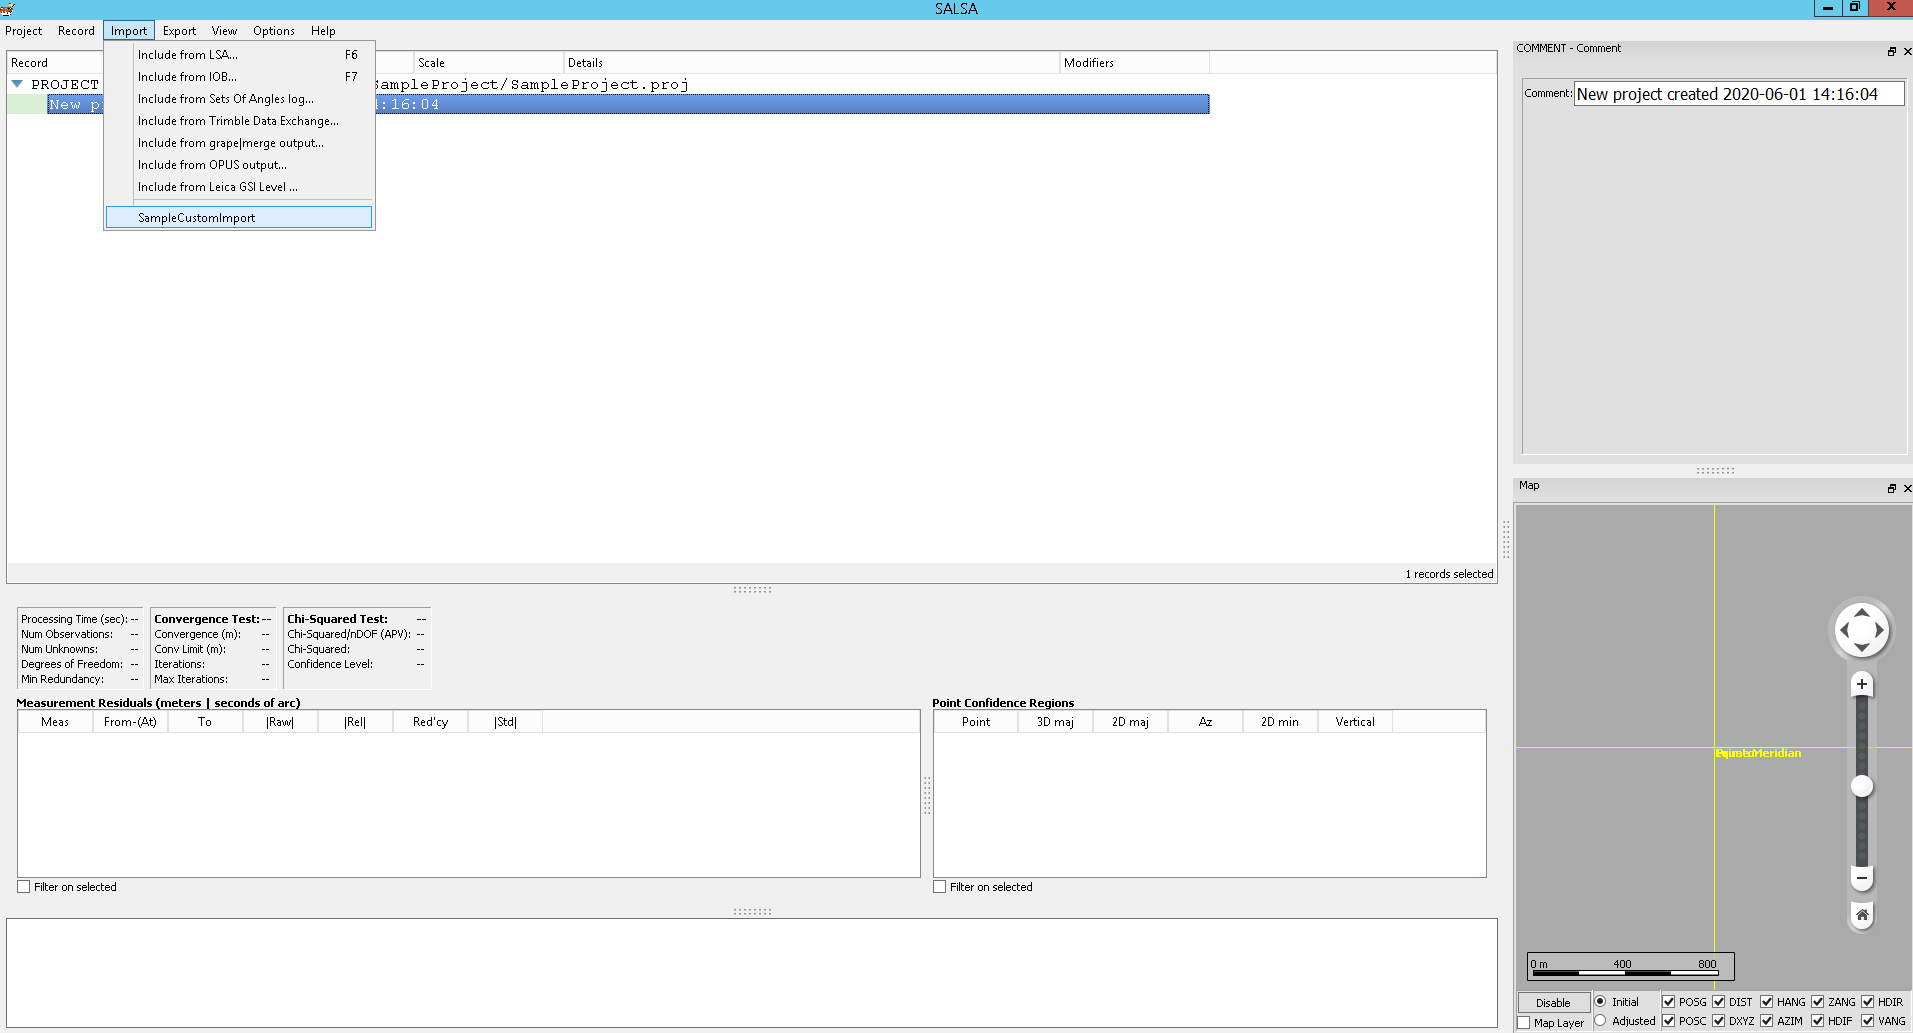
\includegraphics[width=1\textwidth]{customImport.png}\\
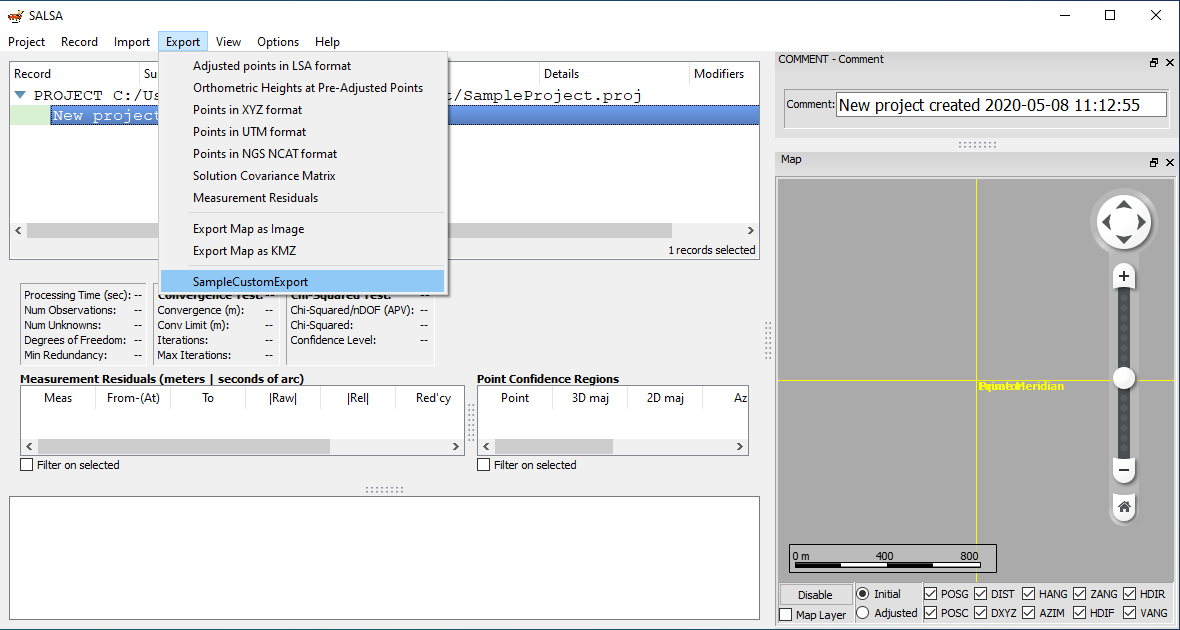
\includegraphics[width=1\textwidth]{customExport.png}
\caption{Scripts placed in discoverable directories will auto-populate as menu actions.}
\label{Fig:customImportExportGUI}
\end{figure}

\section{Writing Custom Import Scripts}

To assist you in writing your own importing scripts, we have provided an example import script, called SampleCustomImport.py.  This file demonstrates how to accept the arguments passed to import scripts from SALSA, manipulate data in an instrument file (such as systematically altering a naming convention) and finally convert it to lsa format.  The arguments passed to these scripts include the path of the general converting tool used by SALSA which currently support Leica GSI, WIPPS PPP, Leica sets of angles (.log), and Trimble Data Exchange Format for GPS, level, total station measurements (.asc).  Users do not need to use these arguments if they prefer to write their own script from scratch.  In the custom import script, the ``Parse'' section shows how to accept the arguments passed by SALSA to the script and should not be heavily modified.  The section ``converterlauncher.py'' shows how to call the usual SALSA import tool with your modified instrument files.  Note that one of the arguments is "type" of the instrument files which may be needed to be modified by the user.

\section{Writing Custom Export Scripts}

To assist you in writing your own reporting scripts, we have provided an example reporting script called SampleCustomExport.py.  This file demonstrates how to use the hdf file which SALSA passes to all reporting scripts to perform manipulations to your output and write out a new file.  The different sections of the scripts are clearly labelled allowing you to only re-use the parts which are relevant for your application.  In particular, the ``Parse'' section, which shows how to accept the hdf file from SALSA, should not be greatly modified.  Furthermore, the ``ReadHDF'' section provides a quick reference for how to extract information from the hdf file and store it into memory.
\section{Obtaining Custom Scripts}

The user is most likely to obtain a custom script either from colleagues or from making it on their own for their special application.  However, there will be a small number of custom scripts which are included in the SALSA release and have been subject to our testing.  The custom export scripts may typically be found in\\
\begin{center}\verb+C:\Program Files\SALSA\reporting\extras+\end{center}
and the custom import scripts may typically be found in\\
\begin{center}\verb+C:\Program Files\SALSA\converters\extras+.\end{center}
To utilize these scripts, they must be copy and pasted in the relevant folders described in \ref{sec:discoverableScripts}.

\section{Facilitating Custom Import and Export File Copies}

If a custom import or export script becomes a common part of the user's workflow, it may become tedious to create subdirectories and copy over the necessary files for each new project. SALSA provides users with a straightforward mechanism to specify files that are automatically added to any newly created project's customImport or customExport folder. Users can accomplish this by completing the following steps.

\begin{enumerate}
	\item Navigate to the \verb+data+ folder in SALSA's installation directory. See Figure \ref{fig:InstallLocations}
	\item Open default.cfg in a text editor. This may require elevated permissions.
	\item Add a new line with the tag \verb+--customExportCopy+ followed by a space and the file name you wish to add to your project's customExport folder. Create a new line for each file you wish to copy into customExport. Note if a file name has a space in it, please enclose in quotes.
	\item Add a new line with the tag \verb+--customImportCopy+ followed by a space and the file name you wish to add to your project's customImport folder. Create a new line for each file you wish to copy into customImport. Note if a file name has a space in it, please enclose in quotes.
	\item Save the modified default.cfg file when finished.
\end{enumerate}

If one or more files are tagged with customExportCopy, a customExport folder is generated when creating a new SALSA project, and the relevant files are copied into that folder. The same paradigm holds for customImport. Note that only new projects will employ these tags in the default.cfg file to automatically copy the files. Users with prior existing projects who wish to employ custom export or custom import scripts must add them manually as described in \ref{sec:discoverableScripts}.




\chapter{LSA Record Reference}
\label{chap:LsaRecordGuide}

It should be clear to the reader at this point in this text that \textsf{salsa} organizes the least squares problem as a collection of what we've been calling ``records,'' that these records may be organized hierarchically, that they may be edited via the Record Editor, and that they are saved with the \textsf{salsa} project in a special \verb+.lsa+ format (which is detailed in Chapter \ref{chap:LsaFormat}).  However, we have not yet introduced all of the record types which may be used in \textsf{salsa}, nor have we fully explained all the fields presented by the Record Editor for each record type.  The goal of this chapter is to provide a complete reference that explains each \textsf{salsa} record type in detail.


Each of the following sections adheres to a consistent pattern: we introduce each record type by its few-letter abbreviation and its one-line description, we explain the fields that are presented in the Record Editor for the record type, and then we close with additional explanation as warranted.  The order of the following sections mirrors the order that record types are shown in \textsf{salsa}'s Record $\to$ Insert menu.


%-----------------------------------------------
% INCLUDE
%-----------------------------------------------
\newpage
\section{INCLUDE - Additional .lsa file}

A special record used to include additional \verb+.lsa+ files in the project.

\subsection*{Record Editor Fields}

\begin{description}[leftmargin=!,labelwidth=\widthof{\bfseries Enabled:}]
\item[Enabled:] When checked, the record will be included in the network adjustment
\item[File:] Relative path to the file to include\textsuperscript{1,2}
\item[Scaling:] Variance scaling to apply to all measurements in the included file\textsuperscript{3}
\end{description}

\subsection*{Notes}
\begin{enumerate}
\item ``Including'' an \verb+.lsa+ file in a \textsf{salsa} project does not affect the file's location.  \textsf{salsa} will read from \emph{and write to} the file wherever it may be located.  Thus, to eliminate the possibility of making unintended changes to files outside of the current \textsf{salsa} project folder, we recommend copying these input files into the \textsf{salsa} project folder and them including them from there.
\item Included files located in the project directory or a child of the project directory are stored with a relative path from the parent file to the included file.  Files located outside of the project directory are stored with an absolute path.
\item Keep in mind the fact that variance scaling in \textsf{salsa} is cumulative, so the effective variance scaling for any record is the product of that individual record's scaling factor times its parent's scaling factor times that parent's scaling factor, etc. 
\end{enumerate}


%-----------------------------------------------
% COMMENT
%-----------------------------------------------
\hrulefill
\section{COMMENT - a comment}

A comment.

\subsection*{Record Editor Fields}

\begin{description}[leftmargin=!,labelwidth=\widthof{\bfseries Comment:}]
\item[Comment:] Text of the comment
\end{description}

\subsection*{Notes}
\begin{enumerate}
\item Comments have no impact on the adjustment; they are supported to help users build a well-organized and well-documented LSA project.
\item A separator bar (also available in the Record $\to$ Insert menu) is just a comment containing a bunch of `--' characters.
\end{enumerate}


%-----------------------------------------------
% POSG
%-----------------------------------------------
\newpage
\section{POSG - Station Position (Geodetic)}

An initial position estimate for a point, using Geodetic coordinates\textsuperscript{1}.

\subsection*{Record Editor Fields}

\begin{description}[leftmargin=!,labelwidth=\widthof{\bfseries Covariance3:}]
\item[Enabled:] When checked, the record will be included in the network adjustment
\item[Label:] Unique string used to describe this point. 
\item[Latitude, Longitude:] Geodetic latitude and longitude of the point.  These angles may be expressed in either degrees, minutes, and seconds of arc (DMS) or as decimal degrees by selecting the corresponding radio button.  Latitudes may be expressed as positive-North or positive South using the N/S selector, and likewise longitudes may be expressed as positive East or West using the E/W selector.
\item[Height:] Height of the point, recorded as either `Ellipsoidal' or `Orthometric'. If the right-most dropdown box is set to `Ellipsoidal', then height is relative to the WGS 84 ellipsoid. If set to `Orthometric', then the height is relative to the geoid defined by the geoid file used in the project.
\item[Type\textsuperscript{2}:] Type(s) of constraints applied to this point \\
  \textbf{Floating:} free to adjust \\
  \textbf{Constrained:} constrained by a covariance matrix \\
  \textbf{Fixed:} Lat, Lon and ElHt are all fixed, point will not be adjusted
\item[Covariance\textsuperscript{3}:] Upper triangular covariance matrix elements
\item[Lat Fixed:] Latitude of the point is fixed and will not be adjusted
\item[Lon Fixed:] Longitude of the point is fixed and will not be adjusted
\item[ElHt Fixed:] Ellipsoid height of the point is fixed and will not be adjusted
\item[Scaling:] Apply a scale factor to multiply the covariance 
\end{description}

\subsection*{Notes}
\begin{enumerate}
\item Note that all internal computations in \textsf{salsa} are executed in an ECEF Cartesian (XYZ) frame; \textsf{salsa} uses the WGS 84 ellipsoid parameters to compute the Cartesian coordinates for POSG records.

\item The `Type' options for POSG (and POSC) records warrant some elaboration.  `Floating' means that the point is entirely free to move in the adjustment, barring any `fixed' components discussed momentarily; any covariance matrix content is ignored.  Most points in a typical survey will be Floating.  `Constrained' means that the point is an absolute ECEF coordinate estimate, complete with a covariance matrix characterizing the uncertainty in that estimate.  Constrained points will move as part of the least squares adjustment just like any other measurement.  `Fixed' means the point's coordinates are taken as known, and they are not allowed to move in the adjustment.  In terms of least squares theory, a fixed point's coordinates are not even included in the state vector which is the subject of the estimation.  `Lat/Lon/ElHt Fixed' technically does not `fix' the point's coordinates but imposes a constraint equation that prohibits movement in the specified direction(s).  The word `fixed' is used in the GUI with some reservation by the authors, but it is concise.

\item Units of the covariance matrix elements are assumed to match the linear units specifying the ellipsoid height.  For example, if the ellipsoid height is expressed in meters, the covariance elements will be interpreted as $\mathrm{m}^2$.  Note that the covariance elements for a POSG record are expressed in a local north/east/up frame as indicated by the matrix element labels.

\end{enumerate}


%-----------------------------------------------
% POSC
%-----------------------------------------------
\newpage
\section{POSC - Station Position (Cartesian)}
An initial position estimate for a point, using ECEF XYZ coordinates.
\subsection*{Record Editor Fields}
\begin{description}[leftmargin=!,labelwidth=\widthof{\bfseries Covariance2:}]
\item[Enabled:] When checked, the record will be used to calculate the network adjustment
\item[Label:] Unique string used to describe this point
\item[X,Y,Z:] ECEF X, Y, and Z coordinate estimates for this point
\item[Type\textsuperscript{1}:] Type(s) of constraints applied to this point \\
  \textbf{Floating:} free to adjust \\
  \textbf{Constrained:} constrained by a covariance matrix \\
  \textbf{Fixed:} Lat, Lon and ElHt are all fixed, point will not be adjusted
\item[Covariance\textsuperscript{2}:] Upper triangular covariance matrix elements
\item[Lat Fixed:] Latitude of the point is fixed and will not be adjusted
\item[Lon Fixed:] Longitude of the point is fixed and will not be adjusted
\item[ElHt Fixed:] Ellipsoid height of the point is fixed and will not be adjusted
\item[Scaling:] Apply a scale factor to multiply the covariance 
\end{description}

\subsection*{Notes}
\begin{enumerate}
\item The `Type' options for POSC (and POSG) records warrant some elaboration.  `Floating' means that the point is entirely free to move in the adjustment, barring any `fixed' components discussed momentarily; any covariance matrix content is ignored.  Most points in a typical survey will be Floating.  `Constrained' means that the point is an absolute ECEF coordinate estimate, complete with a covariance matrix characterizing the uncertainty in that estimate.  Constrained points will move as part of the least squares adjustment just like any other measurement.  `Fixed' means the point's coordinates are taken as known, and they are not allowed to move in the adjustment.  In terms of least squares theory, a fixed point's coordinates are not even included in the state vector which is the subject of the estimation.  `Lat/Lon/ElHt Fixed' technically does not `fix' the point's coordinates but imposes a constraint equation that prohibits movement in the specified direction(s).  The word `fixed' is used in the GUI with some reservation by the authors, but it is concise.
\item Units of the covariance matrix elements are assumed to match those linear units specifying the ECEF XYZ coordinates.  For example, if the ECEF XYZ position is expressed in meters, the covariance elements will be interpreted as $\mathrm{m}^2$.
\end{enumerate}


%-----------------------------------------------
% DIST
%-----------------------------------------------
\newpage
\section{DIST - Distance measurement}

A slant distance measurement between two points.

\subsection*{Record Editor Fields}

\begin{description}[leftmargin=!,labelwidth=\widthof{\bfseries Height From1:}]
\item[Enabled:] When checked, the record will be included in the network adjustment
\item[From:] Label for the point where the measurement vector originates
\item[To:] Label for the point where the measurement vector terminates
\item[Distance:] Distance measured between the From and To points
\item[Sigma:] Measurement uncertainty
\item[Height From\textsuperscript{1}:] Height of the instrument at the From point
\item[Height To:] Height of the target at the To point
\item[Uncertainty:] Uncertainty model to apply to this measurement
\item[Scaling:] Scaling to apply to this measurement's covariance
\end{description}

\subsection*{Notes}
\begin{enumerate}
\item If a distance measurement has already been corrected to account for heights of instrument and target (i.e., ``reduced mark-to-mark''), the Height From/To should be set to zero in \textsf{salsa}.
\end{enumerate}


%-----------------------------------------------
% DXYZ
%-----------------------------------------------
\newpage
\section{DXYZ - Delta XYZ measurement}

An ECEF XYZ vector measurement between two points.

\subsection*{Record Editor Fields}

\begin{description}[leftmargin=!,labelwidth=\widthof{\bfseries Height From2:}]
\item[Enabled:] When checked, the record will be included in the network adjustment
\item[From:] Label for the point where the measurement vector originates
\item[To:] Label for the point where the measurement vector terminates
\item[Delta X,Y,Z:] X,Y,Z components of the vector measurement
\item[Covariance\textsuperscript{1}:] Covariance matrix for the measurement
\item[Height From\textsuperscript{2}:] Height of the instrument at the From point
\item[Height To:] Height of the instrument at the To point
\item[Uncertainty:] Uncertainty model to apply to this measurement
\item[Scaling:] Scaling to apply to this measurement's covariance
\end{description}

\subsection*{Notes}
\begin{enumerate}
\item Units of the covariance matrix elements are assumed to match those linear units specifying the XYZ vector components.  For example, if the vector measurement is expressed in meters, the covariance elements will be interpreted as $\mathrm{m}^2$.
\item If a vector measurement has already been corrected to account for instrument heights (i.e., ``reduced mark-to-mark''), the Height From/To should be set to zero in \textsf{salsa}.  Typically, GNSS processing software does account for instrument heights (as well as antenna effects) when computing the vector estimate.
\end{enumerate}


%-----------------------------------------------
% HANG
%-----------------------------------------------
\newpage
\section{HANG - Horizontal Angle Measurement}

A horizontal angle measured between two points.

\subsection*{Record Editor Fields}

\begin{description}[leftmargin=!,labelwidth=\widthof{\bfseries Height From:}]
\item[Enabled:] When checked, the record will be included in the network adjustment
\item[From:] Label for the point where the angle originates
\item[At:] Label for the point where the instrument is located
\item[To:] Label for the point where the angle terminates
\item[Angle\textsuperscript{1}:] Angle measured between the From and To points
\item[Sigma:] Measurement uncertainty
\item[Height From:] Height of the instrument at the From point
\item[Height To:] Height of the instrument at the To point
\item[Uncertainty:] Uncertainty model to apply to this measurement
\item[Scaling:] Scaling to apply to this measurement's covariance
\item[Reduced:] When checked, indicates measurement has been reduced to the Ellipsoid
\end{description}

\subsection*{Notes}
\begin{enumerate}
\item The sign convention for horizontal angles is positive-clockwise.
\end{enumerate}


%-----------------------------------------------
% AZIM
%-----------------------------------------------
\newpage
\section{AZIM - Azimuth Measurement}

A horizontal angle measured\textsuperscript{1} from the North\textsuperscript{2} vector.

\subsection*{Record Editor Fields}

\begin{description}[leftmargin=!,labelwidth=\widthof{\bfseries Refract Coeff:}]
\item[Enabled:] When checked, the record will be included in the network adjustment
\item[From:] Label for the point at which the azimuth was observed
\item[To:] Label for the point that was the target of the azimuth observation
\item[Angle:] Angle from true North to the To point\textsuperscript{2}
\item[Sigma:] Measurement uncertainty
\item[Height From:] Height of the instrument at the From point
\item[Height To:] Height of the target at the To point
\item[Uncertainty:] Uncertainty model to apply to this measurement
\item[Scaling:] Scaling to apply to this measurement's covariance
\item[Reduced:] When checked, indicates measurement has been reduced to the Ellipsoid
\end{description}

\subsection*{Notes}
\begin{enumerate}
\item Azimuth `measurements' are not, in practice, observed directly.  Rather, they are the product of other measurements and reductions typically including astronomic observations.  These estimates may be introduced into \textsf{salsa} as an AZIM record.  The sign convention for azimuths is positive-clockwise.
\item The default convention for Azimuth records is that they are expressed as angles clockwise from North; this record provides an option to instead specify the angle clockwise from South.
\end{enumerate}


%-----------------------------------------------
% VANG
%-----------------------------------------------
\newpage
\section{VANG - Vertical Angle Measurement}

An angle measurement of a point relative to the horizontal plane\textsuperscript{1}.

\subsection*{Record Editor Fields}

\begin{description}[leftmargin=!,labelwidth=\widthof{\bfseries Refract Coeff:}]
\item[Enabled:] When checked, the record will be included in the network adjustment
\item[From:] Label for the point at which the measurement is taken
\item[To:] Label for the point where the angle terminates
\item[Angle:] Angle measured from the horizontal plane to the To point
\item[Sigma:] Measurement uncertainty
\item[Height From:] Height of the instrument at the From point
\item[Height To:] Height of the target at the To point
\item[Uncertainty:] Uncertainty model to apply to this measurement
\item[Refract Coeff:] Coefficient used for refraction correction\textsuperscript{2}
\item[Scaling:] Scaling to apply to this measurement's covariance
\item[Reduced:] When checked, indicates measurement has been reduced to the \\Ellipsoid\textsuperscript{3}
\end{description}

\subsection*{Notes}
\begin{enumerate}
\item Vertical and Zenith angles are complementary; a VANG record with observed angle $\alpha$ is exactly equivalent to a ZANG record with observed angle $90 - \alpha$.
\item Empirical studies of terrestrial refraction, $k$, show that the frequently-used Gaussian refraction coefficient of $k=0.13$ is not suitable for describing refraction effects in the lower atmosphere (where surveying observations are taken) and that $k$ can vary from -4 to +16 over the course of a day \cite{Hirt}.  \textsf{salsa} users are advised to leave the refraction correction disabled (equivalent to $k=0$) in the absence of comprehensive atmospheric data concurrent with their observations.
\item Typically, VANG/ZANG observations are not reduced to the Ellipsoid; they are made relative to the local gravity field and are influenced by any deflection of the vertical (DOV) at the instrument location.  Unless the user specifies that the measurement has already been reduced to the Ellipsoid, \textsf{salsa} will apply DOV corrections to the observation.
\end{enumerate}


%-----------------------------------------------
% ZANG
%-----------------------------------------------
\newpage
\section{ZANG - Zenith Angle Measurement}

An angle measurement of a point relative to vertical\textsuperscript{1}.

\subsection*{Record Editor Fields}

\begin{description}[leftmargin=!,labelwidth=\widthof{\bfseries Refract Coeff:}]
\item[Enabled:] When checked, the record will be included in the network adjustment
\item[From:] Label for the point at which the measurement is taken
\item[To:] Label for the point where the angle terminates
\item[Angle:] Angle measured from the vertical axis to the To point
\item[Sigma:] Measurement uncertainty
\item[Height From:] Height of the instrument at the From point
\item[Height To:] Height of the target at the To point
\item[Uncertainty:] Uncertainty model to apply to this measurement
\item[Refract Coeff:] Coefficient used for refraction correction\textsuperscript{2}
\item[Scaling:] Scaling to apply to this measurement's covariance
\item[Reduced:] When checked, indicates measurement has been reduced to the \\Ellipsoid\textsuperscript{3}
\end{description}

\subsection*{Notes}
\begin{enumerate}
\item Vertical and Zenith angles are complementary; a VANG record with observed angle $\alpha$ is exactly equivalent to a ZANG record with observed angle $90 - \alpha$.
\item Empirical studies of terrestrial refraction, $k$, show that the frequently-used Gaussian refraction coefficient of $k=0.13$ is not suitable for describing refraction effects in the lower atmosphere (where surveying observations are taken) and that $k$ can vary from -4 to +16 over the course of a day \cite{Hirt}.  \textsf{salsa} users are advised to leave the refraction correction disabled (equivalent to $k=0$) in the absence of comprehensive atmospheric data concurrent with their observations.
\item Typically, VANG/ZANG observations are not reduced to the Ellipsoid; they are made relative to the local gravity field and are influenced by any deflection of the vertical (DOV) at the instrument location.  Unless the user specifies that the measurement has already been reduced to the Ellipsoid, \textsf{salsa} will apply DOV corrections to the observation.
\end{enumerate}


%-----------------------------------------------
% HDIF
%-----------------------------------------------
\newpage
\section{HDIF - Height Difference Measurement}

A measure of the difference between two heights.

\subsection*{Record Editor Fields}

\begin{description}[leftmargin=!,labelwidth=\widthof{\bfseries Refract Coeff:}]
\item[Enabled:] When checked, the record will be included in the network adjustment
\item[From:] Label for the point from which the height difference is referenced
\item[To:] Label for the point referenced by the height difference
\item[Height Diff:] Measured height difference between the From and To points
\item[Sigma:] Measurement uncertainty
\item[Uncertainty:] Uncertainty model to apply to this measurement
\item[Refract Coeff:] Coefficient used for refraction correction\textsuperscript{1}
\item[Scaling:] Scaling to apply to this measurement's covariance
\item[Reduced:] When checked, indicates measurement has been reduced to the \\Ellipsoid\textsuperscript{2}
\item[Curvature:] When checked, indicates that the curvature correction will be applied
\item[OHC:] When checked, indicates that the orthometric height correction will be applied
\end{description}

\subsection*{Notes}
\begin{enumerate}
\item Empirical studies of terrestrial refraction, $k$, show that the frequently-used Gaussian refraction coefficient of $k=0.13$ is not suitable for describing refraction effects in the lower atmosphere (where surveying observations are taken) and that $k$ can vary from -4 to +16 over the course of a day \cite{Hirt}.  \textsf{salsa} users are advised to leave the refraction correction disabled (equivalent to $k=0$) in the absence of comprehensive atmospheric data concurrent with their observations.
\item Typically, leveling measurements have not been reduced to the Ellipsoid prior to importing them in \textsf{salsa}; they are therefore orthometric height differences, and \textsf{salsa} will apply gravity corrections to these observations.  If the observation has already been reduced outside of \textsf{salsa} (thus it represents an ellipsoid height difference), this box should be checked so that \textsf{salsa} does not apply gravity corrections.
\end{enumerate}


%-----------------------------------------------
% HDIR
%-----------------------------------------------
\newpage
\section{HDIR - Horizontal Direction Measurement}

A measurement that defines a direction to a point\textsuperscript{1}.

\subsection*{Record Editor Fields}

\begin{description}[leftmargin=!,labelwidth=\widthof{\bfseries Height To:}]
\item[Enabled:] When checked, the record will be included in the network adjustment
\item[To Point:] Label for the point to which this direction is measured
\item[Dir Group:] Label for the Direction Group this direction belongs to
\item[Angle:] The measured direction angle
\item[Sigma:] Measurement uncertainty
\item[Height To:] Height of the target at the To point
\end{description}

\subsection*{Notes}
\begin{enumerate}
\item Unlike azimuth observations (AZIM) which are relative to true North, horizontal direction records (HDIR) in \textsf{salsa} are relative to an arbitrary azimuth defined by the instrument (typically a total station).  As such, HDIR records are only meaningful when expressed as a group; see the Direction Group (DGRP) record introduced next.
\end{enumerate}


%-----------------------------------------------
% DGRP
%-----------------------------------------------
\newpage
\section{DGRP - Direction Group}

A group that comprises a set of horizontal direction measurements.

\subsection*{Record Editor Fields}

\begin{description}[leftmargin=!,labelwidth=\widthof{\bfseries Uncertainty:}]
\item[Enabled:] When checked, the record will be included in the network adjustment
\item[Label:] Unique string used to describe this direction group
\item[At Point:] Label for the point at which directions in this group were measured
\item[Uncertainty:] Uncertainty model to apply to these measurements
\item[Scaling:] Scaling to apply to these measurements' covariance
\item[Reduced:] When checked, indicates measurement has been reduced to the Ellipsoid
\end{description}

\subsection*{Notes}
\begin{enumerate}
\item Reference the HDIR record discussed on the previous page.
\end{enumerate}


%-----------------------------------------------
% HGHT
%-----------------------------------------------
\newpage
\section{HGHT - Height of Instrument/Target}

A record used to capture instrument and target heights.

\subsection*{Record Editor Fields}

\begin{description}[leftmargin=!,labelwidth=\widthof{\bfseries Enabled:}]
\item[Enabled:] When checked, the record will be included in the network adjustment
\item[Label:] Unique label used to identify this height record
\item[Height:] The height of the instrument or target for this correction
\end{description}

\subsection*{Notes}
\begin{enumerate}
\item Like other `modifier' records in \textsf{salsa}, the HGHT record exists so that other \textsf{salsa} records can reference it.
The purpose of the HGHT record is to capture the numeric height of instrument or target for a particular setup; then all observations
taken with that setup -- assuming they have not already been reduced mark-to-mark -- should reference a common HGHT record.  This `best practice' keeps \textsf{salsa} projects clear and maintainable.
\end{enumerate}


%-----------------------------------------------
% VSCA
%-----------------------------------------------
\newpage
\section{VSCA - Variance Scaling}

A record used to provide additional scaling to the variance (sigma$^2$ or covariance) of a measurement.

\subsection*{Record Editor Fields}

\begin{description}[leftmargin=!,labelwidth=\widthof{\bfseries Enabled:}]
\item[Enabled:] When checked, the record will be included in the network adjustment
\item[Label:] Unique label used to identify this record
\item[Scaling:] Variance scaling to apply to the measurement
\end{description}

\subsection*{Notes}
\begin{enumerate}
\item Note that individual measurement records, as well as INCLUDE records, can be scaled directly by entering a numeric value.  The purpose of the VSCA record, like other `modifiers' in \textsf{salsa}, is to allow a user to create a descriptively-named record that can be referenced by other records.  For example, in a large project containing many files a user might create a VSCA record named ``GPS'' and another named ``Conventional'' and then reference the appropriate VSCA record in each INCLUDE record in the project.  This `best practice' simplifies any subsequent tuning of the relative variances among GPS and conventional observations.
\item A VSCA record is also the only way to scale the entire project; the top-level project record (which in all other ways is identical to an INCLUDE record) does not support numeric variance scaling but can reference a VSCA record.
\end{enumerate}


%-----------------------------------------------
% UNCR
%-----------------------------------------------
\newpage
\section{UNCR - Uncertainty Model}

An uncertainty model describing sigma, ppm, and centering errors\textsuperscript{1}.

\subsection*{Record Editor Fields}

\begin{description}[leftmargin=!,labelwidth=\widthof{\bfseries From Cent Err:}]
\item[Enabled:] When checked, the record will be included in the network adjustment
\item[Label:] Unique label used to identify this record
\item[At Cent Err:] Centering error to apply at the At point
\item[From Cent Err:] Centering error to apply at the From point
\item[To Cent Err:] Centering error to apply at the To point
\item[PPM:] Parts per million error to apply to the measurement
\item[Sigma:] Additional measurement uncertainty to apply
\end{description}

\subsection*{Notes}
\begin{enumerate}
\item Not all components of an uncertainty model (UNCR record) are applicable to all measurement types.  For example, a DXYZ record is impacted by From and To centering errors, but there is no `At' station.  \textsf{salsa} will apply the applicable components of an UNCR model to records that reference it.
\end{enumerate}


%-----------------------------------------------
% MEAN
%-----------------------------------------------
\newpage
\section{MEAN - Position Derived from Mean of Positions} \label{sect:MEAN}

A MEAN record specifies a derived position that is calculated as the mean of a group of points after the adjustment is completed.  A MEAN record can be edited in the Project Navigator and Record Editor.  The derived position that the MEAN record specifies will appear in the Point Confidence Regions table in the Salsa gui.  It will also appear in the .csv, .pts, and .h5 output files.

\subsection*{Record Editor Fields}

\begin{description}[leftmargin=!,labelwidth=\widthof{\bfseries Positions:}]
\item[Enabled:] When checked, the derived point will be calculated
\item[Label:] Label assigned to the derived point specified by the MEAN record
\item[Positions:] List\textsuperscript{(a)} of POSG and POSC record used in the mean calculation
\end{description}

\subsection*{Derived Position Calculation Details}

The mean derived point is computed as an unweighted mean position of two or more adjusted, fixed, or previously computed derived points.  The mean derived point is calculated after the adjustment is completed.  For example, consider a structure that is surveyed at four corners, as depicted in Figure \ref{Fig:mean4Structure}.  For the mean derived point to correspond to the center of the building, the four corner points must be employed in the unweighted mean computation.  The computed formal uncertainty on the mean point does not account for the possible error introduced by a failure to symmetrically survey the structure.  However, it is possible to add uncertainty $\sigma_{\text{extra}}$ to all components of the mean point (i.e. $\sigma_{\text{extra}}^2$ is added to all three diagonal components of the mean derived point covariance) if the user feels there is unmodeled error in the points used to compute to mean derived point. The mapping of the formal covariance from the included points to the mean derived point is discussed in Appendix ``\nameref{appendices:DerPtUncMapping}''.

\begin{figure}[!htbp]
\centering
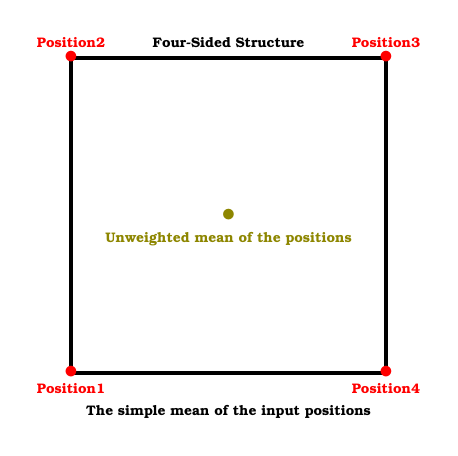
\begin{tikzpicture}
\draw (2,-0.5) node{{\color{black}{\tiny{\textbf{The simple mean of the input positions}}}}};

\draw (2,4.2) node{{\color{black}{\tiny{\textbf{Four-Sided Structure}}}}};
\draw[straight,color=black,line width=0.5mm,solid] (0,0) -- (0,4);
\draw[straight,color=black,line width=0.5mm,solid] (0,4) -- (4,4);
\draw[straight,color=black,line width=0.5mm,solid] (4,4) -- (4,0);
\draw[straight,color=black,line width=0.5mm,solid] (4,0) -- (0,0);


\draw (0,0) node{{\color{red}{$\bullet$}}};
\draw (0,-0.2) node{{\color{red}{\tiny{\textbf{Position1}}}}};
\draw (0,4) node{{\color{red}{$\bullet$}}};
\draw (0,4.2) node{{\color{red}{\tiny{\textbf{Position2}}}}};
\draw (4,4) node{{\color{red}{$\bullet$}}};
\draw (4,4.2) node{{\color{red}{\tiny{\textbf{Position3}}}}};
\draw (4,0) node{{\color{red}{$\bullet$}}};
\draw (4,-0.2) node{{\color{red}{\tiny{\textbf{Position4}}}}};

\draw (2,2) node{{\color{olive}{$\bullet$}}};
\draw (2,1.7) node{{\color{olive}{\tiny{\textbf{Unweighted mean of the positions}}}}};
\end{tikzpicture}~~~
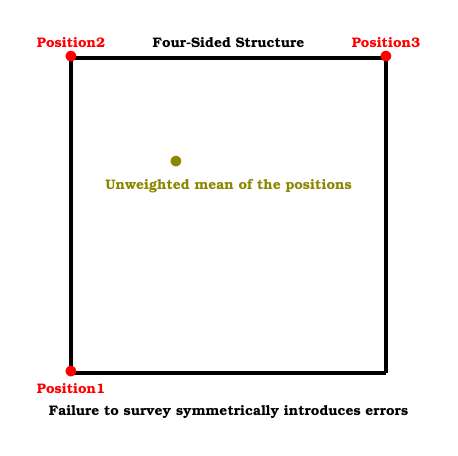
\begin{tikzpicture}
\draw (2,-0.5) node{{\color{black}{\tiny{\textbf{Failure to survey symmetrically introduces errors}}}}};

\draw (2,4.2) node{{\color{black}{\tiny{\textbf{Four-Sided Structure}}}}};
\draw[straight,color=black,line width=0.5mm,solid] (0,0) -- (0,4);
\draw[straight,color=black,line width=0.5mm,solid] (0,4) -- (4,4);
\draw[straight,color=black,line width=0.5mm,solid] (4,4) -- (4,0);
\draw[straight,color=black,line width=0.5mm,solid] (4,0) -- (0,0);


\draw (0,0) node{{\color{red}{$\bullet$}}};
\draw (0,-0.2) node{{\color{red}{\tiny{\textbf{Position1}}}}};
\draw (0,4) node{{\color{red}{$\bullet$}}};
\draw (0,4.2) node{{\color{red}{\tiny{\textbf{Position2}}}}};
\draw (4,4) node{{\color{red}{$\bullet$}}};
\draw (4,4.2) node{{\color{red}{\tiny{\textbf{Position3}}}}};

\draw (1.333,2.667) node{{\color{olive}{$\bullet$}}};
\draw (2,2.367) node{{\color{olive}{\tiny{\textbf{Unweighted mean of the positions}}}}};
\end{tikzpicture}~~~
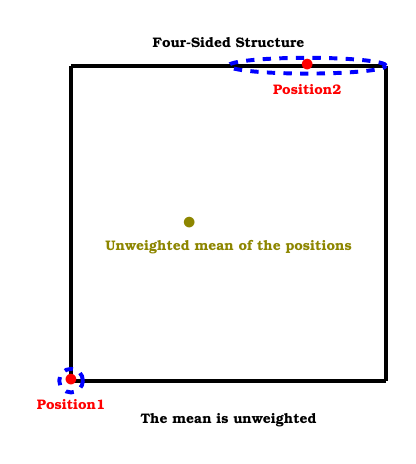
\begin{tikzpicture}
\draw (2,-0.5) node{{\color{black}{\tiny{\textbf{The mean is unweighted}}}}};

\draw (2,4.3) node{{\color{black}{\tiny{\textbf{Four-Sided Structure}}}}};
\draw[straight,color=black,line width=0.5mm,solid] (0,0) -- (0,4);
\draw[straight,color=black,line width=0.5mm,solid] (0,4) -- (4,4);
\draw[straight,color=black,line width=0.5mm,solid] (4,4) -- (4,0);
\draw[straight,color=black,line width=0.5mm,solid] (4,0) -- (0,0);


\draw (0,0) node{{\color{red}{$\bullet$}}};
\draw (0,-0.3) node{{\color{red}{\tiny{\textbf{Position1}}}}};
\draw[straight,color=blue,line width=0.5mm,dashed] (0,0) circle (0.15);
\draw (3,4) node{{\color{red}{$\bullet$}}};
\draw (3,3.7) node{{\color{red}{\tiny{\textbf{Position2}}}}};
\draw[straight,color=blue,line width=0.5mm,dashed] (3,4) circle (1 and 0.1);
\draw (1.5,2) node{{\color{olive}{$\bullet$}}};
\draw (2,1.7) node{{\color{olive}{\tiny{\textbf{Unweighted mean of the positions}}}}};
\end{tikzpicture}
\caption{The unweighted mean will acquire errors if the object of interest is not surveyed symmetrically.  In the left diagram, the four corners of a structure are surveyed and the mean corresponds to the center of the structure.  In the middle diagram, one of the corners of the structure cannot be accessed for survey, and therefore the mean does not correspond to the center of the structure.  In the right diagram, the unweighted mean is not impacted by the blue uncertainty ellipses.}
\label{Fig:mean4Structure}
\end{figure}

\subsection*{Notes}
\begin{enumerate}[label=(\alph*)]
\item In the .lsa file, the list is a space separated list of position labels.  Any position labels containing a space are enclosed in double quotes.
\end{enumerate}


%-----------------------------------------------
% ENUO
%-----------------------------------------------
\newpage
\section{ENUO - Position Derived from ENU Offset from Position} \label{sect:ENUO}

A ENUO record specifies a derived position that is calculated as an East-North-Up offset from an adjusted, fixed, or previously computed derived point.  The ENUO derived point is calculated after the adjustment is completed.  A ENUO record can be edited in the Project Navigator and Record Editor.  The derived position that the ENUO record specifies will appear in the Point Confidence Regions table in the Salsa gui.  It will also appear in the .csv, .pts, and .h5 output files.

\subsection*{Record Editor Fields}

\begin{description}[leftmargin=!,labelwidth=\widthof{\bfseries Positions:}]
\item[Enabled:] When checked, the derived point will be calculated
\item[From:] Label for the adjusted position that defines the origin of the ENU offset
\item[To:] Label assigned to the derived point specified by the ENUO record
\item[Delta E,N,U:] East, North, Up offsets
\item[Sigma E,N,U:] East, North, Up offset uncertainties
\end{description}

\subsection*{Derived Position Calculation Details}

To apply the provided ENU offset vector to the ``from'' point specified and thus obtain the derived point, the ENU offset vector is rotated from the ENU frame to the ECEF XYZ frame and then added to the ECEF XYZ ``from'' point position:
\begin{equation}
\left[\begin{array}{c}X_f\\Y_f\\Z_f\end{array}\right] = \left[\begin{array}{c}X_0\\Y_0\\Z_0\end{array}\right] + \left[\begin{array}{ccc}-\sin\lambda_0&-\cos\lambda_0\sin\phi_0&\cos\lambda_0\cos\phi_0\\\cos\lambda_0&-\sin\lambda_0\sin\phi_0&\sin\lambda_0\cos\phi_0\\0&\cos\phi_0&\sin\phi_0\end{array}\right] \left[\begin{array}{c}\Delta E\\\Delta N\\\Delta U\end{array}\right]
\end{equation}
where $\{X_0,Y_0,Z_0\}$ are the ECEF XYZ coordinates of the ``from'' position and $\{\phi_0,\lambda_0\}$ are the corresponding latitude and longitude values.  The mapping of the formal covariance for the ENUO derived point is discussed in Appendix ``\nameref{appendices:DerPtUncMapping}''.

\newpage \ 


\begin{landscape}
\chapter{The LSA File Format Specification}
\label{chap:LsaFormat}

Note: Legal limits for the strings and numeric values composing LSA records are listed in \verb+lsaValidationSpec.xlsx+,
which is installed along-side this User Manual, in the SALSA documentation folder. The output decimal precision for these values are defined there as well. LSA records that contain
values not conforming to these limits or are otherwise malformed will yield parse warnings in SALSA.

\begin{Snippet}
### Whitespace Delimited ### 
- In general, this syntax is space-delimited.
- Any number of adjacent white space characters (spaces and tabs) will be treated as a single delimiter.
- Any labels or filenames containing spaces must be enclosed in double quotes.
- Blank lines are preserved by the .lsa file parser but not displayed in the salsa gui.
- An exception to this is the text notes field, delimited by its <TXNS> </TXNS> tags.

### Comments and Disabled Records ###
- Any line starting with a # is either a comment or a disabled record.  
- The parser will attempt to parse any line that begins with a # as a record. 
    - If the line parses successfully, the line is stored as a disabled record.  
    - If the parse fails, the line is stored as a comment.

### LSA Record Specifications ###
- In general, one line of the file corresponds to one record.  
- If the parser encounters a record ending with "...", it will continue parsing the record on the next line.
- Each record begins with a unique 4 letter designation for the record type.
- Fields enclosed in <angled braces> are required.
- Fields enclosed in [brackets] are optional.
- The OR symbol (|) indicates a number valid values for a location.
- All records (except comments) having associated General Notes gain the notes field [<TXNS></TXNS>] on save.

### Positions ###
POSG <sta_name> [Flt|Con|Fix][N|E|U] <degrees | D M S> <N|S> <degrees | D M S> <E|W> <Height> <cm|m|ft> [ortho]
[CovNN CovNE CovNU CovEE CovEU CovUU][VSCA<VALUE val>|<label>][AUTOGEN] [<TXNS></TXNS>]

POSC <sta_name> [Flt|Con|Fix][N|E|U] <X Y Z m|km|ft>
[CovXX CovXY CovXZ CovYY CovYZ CovZZ][VSCA<VALUE val>|<label>][AUTOGEN] [<TXNS></TXNS>]

NOTE: the Flt|Con|Fix and N|E|U options for POSG and POSC store the values displayed in the gui. Logically 
incompatible parameter combinations such as 'NE + Fix' are valid and should be fully supported as part 
of the LSA file spec. These inconsistencies are resolved when flattening the LSA tree to the .dat file.

### Measurements ###
DXYZ <FROM> <TO> <dX dY dZ m|km|ft> <cxx cxy cxz cyy cyz czz> 
[HFROM<label>|<ht cm|m|ft hts cm|m|ft>][HTO<label>|<ht cm|m|ft hts cm|m|ft>][UNCR label]
[VSCA<VALUE val>|<label>] [<TXNS></TXNS>]

DIST <FROM> <TO> <distance> <sigma cm|km|m|ft> 
[HFROM<label>|<ht cm|m|ft hts cm|m|ft>][HTO<label>|<ht cm|m|ft hts cm|m|ft>][UNCR label]
[VSCA<VALUE val>|<label>] [<TXNS></TXNS>]

HANG <FROM> <AT> <TO> <degrees> [min sec DMS] <sigma rad|deg|soa> 
[HFROM<label>|<ht cm|m|ft hts cm|m|ft>][HTO<label>|<ht cm|m|ft hts cm|m|ft>][UNCR label][REDUCED]
[VSCA<VALUE val>|<label>] [<TXNS></TXNS>]

ZANG <FROM> <TO> <degrees> [min sec DMS] <sigma rad|deg|soa> 
[HFROM<label>|<ht cm|m|ft hts cm|m|ft>][HTO<label>|<ht cm|m|ft hts cm|m|ft>][UNCR label][REFRACT coeff][REDUCED]
[VSCA<VALUE val>|<label>] 
[<TXNS></TXNS>]

VANG <FROM> <TO> <degrees> [min sec DMS] <sigma rad|deg|soa> 
[HFROM<label>|<ht cm|m|ft hts cm|m|ft>][HTO<label>|<ht cm|m|ft hts cm|m|ft>][UNCR label][REFRACT coeff][REDUCED]
[VSCA<VALUE val>|<label>] 
[<TXNS></TXNS>]

AZIM <FROM> <TO> <N|S> <degrees> [min sec DMS] <sigma rad|deg|soa> 
[HFROM<label>|<ht cm|m|ft hts cm|m|ft>][HTO<label>|<ht cm|m|ft hts cm|m|ft>][UNCR label][REDUCED]
[VSCA<VALUE val>|<label>] [<TXNS></TXNS>]

HDIF <FROM> <TO> <ht diff> <sigma cm|m|ft> 
[UNCR label][REFRACT coeff][REDUCED][VSCA VALUE value | label][CURV] [OHC] [<TXNS></TXNS>]

### Directions and Direction Groups ###
DGRP <dir_group> <AT> [UNCR label][REDUCED][VSCA VALUE value | label] [<TXNS></TXNS>]
HDIR <dir_group> <TO> [*+*|-]<degrees> [min sec DMS] <sigma rad|deg|soa> [HTO <label>|<ht cm|m|ft hts cm|m|ft>]
[<TXNS></TXNS>]

## Modifiers
UNCR <tag> <sigma> <cm|m|ft|rad|deg|soa> <PPM> <AT cent error> <FROM cent error> <TO cent error> <cm|m|ft>
[<TXNS></TXNS>]
VSCA <tag> <scale factor> [TOPARENT] [<TXNS></TXNS>]
HGHT <tag> <height> <cm|m|ft> <heightSigma> <cm|m|ft> [<TXNS></TXNS>]

## Derived Measurements
MEAN <NEW_POINT> <sigma cm|km|m|ft> [POINT] [POINT] [POINT] ... [<TXNS></TXNS>]
ENUO <FROM> <NEW_POINT> <dE dN dU m|km|ft> <se sn su> [<TXNS></TXNS>]
\end{Snippet}
\end{landscape}





\chapter{The DAT File Format Specification}
\label{chap:datref}

The solver input data is contained in a flat text file (the ``DAT file,'' usually with extension \verb+.dat+) with its own format as documented here.

Notes on the format:
\begin{Snippet}
# DAT files are ASCII and whitespace-delimited with one record per line
# Labels (From, At, To) denote positions (Points or POS records)
# Each POS record (Point) must have a unique label;
#    but not all labels need have a POS record.
# keywords are in ALL CAPS
# POS ... CONS c[c'] constrain the position solution to a plane[line]
#    using c,c' = one of{XYZ} OR {NEU} and c != c'
# Note that covariance is required for POS with ADJ
# FIX : Point is constant (not adjusted);
# ADJ : use position as a priori information and adjust control point;
# EST or blank: use position only as a priori.
# LUNIT means linear unit MM|M|CM|KM|FT
# AUNIT means angular unit RAD|DEG|SOA but not DMS
# DMS denotes 'deg/min/sec' (int/int/float) and follows angle given by deg min sec
# NB in the angle records "angle sig AUNIT" means angle and sigma
#   both have unit AUNIT; consider "angle AUNIT sig AUNIT"
# fcsig acsig and tcsig are centering errors on From, At and To stations in LUNITs
# CORR is optional but must be followed by corrections in the order shown;
#   use zero placeholders.
# ht[f|t] is height at From|To; target height diff. is implemented using From+To
# refract is a float refraction, and CURV, OHC and GEOID are keywords meaning
#    apply curvature, orthometric height and (DOV, undulation) corrections,
#    respectively.
# Title is for output only
# comment lines begin with '#' and are ignored; also #-to-EOL is ignored
#
# Tags: each measurement record (all measurements+DirSet+Dir+POS ADJ)
#   can be given an optional tag with the field tag=TAG
#  where TAG is the user's tag. This field MUST BE THE LAST FIELD on the line.
#   This tag will be used in generating
#  "data names" in the solver, rather than simply numbering them;
#   the number will be used when a tag is not found.
#  The user MUST use unique tags; failure to do so will cause the solver
#   to throw an exception.
\end{Snippet}

The records are defined as follows, each a single line (even though some lines here are wrapped), beginning with a keyword.

Configuration records.
\begin{Snippet}
# Configuration: output precision; problem dimension (2D is XY);
#   convergence criteria
TITLE title # quotes optional
PREC  eps UNIT [eps UNIT] # output precision; linear and/or angular units
DIM 2|3  # dimension of the problem; 2D is XY only, i.e. Z's ignored
CONV [n ITER] [d CONV] # convergence criteria; either or both
CONFIDENCE alpha       # confidence for Chi squ test (0 < alpha < 1)
OUT [NOAPV] [APQUIT]   # output NOAPV = do not scale covariance with APV
OUT [NOAPV] [APQUIT]   # output APQUIT = quit after ComputeAPriori()
GEOIDFILE filename     # Filename for the gridded EGM08 geoid file
INTERPOLATION method   # Geoid Interpolation method (bicubic, bilinear)
HASH string            # GUI may want to pass hash through solver to binary file
COMMENT ...            # comment that is echoed in output file
GEOID <file>           # geoid file
\end{Snippet}

Position (site or Point) record.
\begin{Snippet}
# no corrections; constraints c one[two] of XYZ|NEU
POS label X Y Z [covxx xy xz yy yz zz] LUNIT [FIX|ADJ|EST] [CONS c[c]]
# undocumented
POS label D M S N|S D M S E|W Ht LUNIT [covxx xy xz yy yz zz [NEU] LUNIT]
         [FIX|ADJ|EST] [CONS c[c]]

POS label X Y Z covxx xy xz yy yz zz LUNIT FIX|ADJ|EST CONS c[c]
POS label X Y Z covxx xy xz yy yz zz LUNIT FIX|ADJ|EST
POS label X Y Z covxx xy xz yy yz zz LUNIT             CONS c[c]
POS label X Y Z LUNIT                      FIX|EST     CONS c[c]
POS label X Y Z LUNIT                      FIX|EST
POS label X Y Z LUNIT                                  CONS c[c]
POS label D M S N|S D M S E|W Ht LUNIT covxx xy xz yy yz zz NEU LUNIT FIX|ADJ|EST
         CONS c[c]
POS label D M S N|S D M S E|W Ht LUNIT covxx xy xz yy yz zz NEU LUNIT FIX|ADJ|EST
POS label D M S N|S D M S E|W Ht LUNIT covxx xy xz yy yz zz NEU LUNIT            
         CONS c[c]
POS label D M S N|S D M S E|W Ht LUNIT covxx xy xz yy yz zz     LUNIT FIX|ADJ|EST
         CONS c[c]
POS label D M S N|S D M S E|W Ht LUNIT covxx xy xz yy yz zz     LUNIT FIX|ADJ|EST
POS label D M S N|S D M S E|W Ht LUNIT covxx xy xz yy yz zz     LUNIT            
         CONS c[c]
POS label D M S N|S D M S E|W Ht LUNIT                                FIX|EST    
         CONS c[c]
POS label D M S N|S D M S E|W Ht LUNIT                                FIX|EST
POS label D M S N|S D M S E|W Ht LUNIT                                           
         CONS c[c]
\end{Snippet}

Measurement records (again, one per line even though some are wrapped here).
\begin{Snippet}
# 3-D delta XYZ (Delta)
DEL labFr labTo dX dY dZ covxx xy xz yy yz zz [asig [PPM]] [fcsig tcsig] LUNIT
        [CORR htf htt [LUNIT]]

# Distance (Dist)
DIS labFr labTo distance sig [asig [PPM]] [fcsig tcsig] LUNIT
        [CORR htf htt [LUNIT] [refract]]

# height (Height) GEOID if orthometric and undulation correction must be applied
HGT labFr labTo height sig [asig [PPM]] LUNIT [CORR [refract]
        [CURV] [GEOID]]

# Azimuth (Azimuth)
AZM labFr labTo angle [min sec DMS|AUNIT] sig [asig] AUNIT [fcsig tcsig LUNIT]
        [CORR htf htt [LUNIT] [GEOID]]

# Horizonal angle (HAngle)
HAN labFr labAt labTo angle [min sec DMS|AUNIT] sig [asig] AUNIT [fc ac tc LUNIT]
        [CORR htf htt [LUNIT] [GEOID]]

# Direction set and Direction (each complete set used to create set of HANs)
# Set = { One DIRSET + >1 DIR with one "group" string};
#   group for each set must be unique and identical throughout set
# Zero or one DIR in a set -> set is ignored - no HANs can be constructed
# DIRs where group does not appear in a DIRSET are ignored
DIRSET group labAt [ac LUNIT] [CORR GEOID]
DIR group labTo angle [min sec DMS|AUNIT] sig [asig] AUNIT [tc LUNIT]
        [CORR htt [LUNIT]]

# Vertical angle (VAngle)
VAN labFr labTo angle [min sec DMS|AUNIT] sig [asig] AUNIT [fc tc LUNIT]
        [CORR htf htt [LUNIT] [refract] [GEOID]]

# Zenith angle (ZAngle)
ZAN labFr labTo angle [min sec DMS|AUNIT] sig [asig] AUNIT [ac tc LUNIT]
        [CORR htf htt [LUNIT] [refract] [GEOID]]
\end{Snippet}

A table showing which records have centering, sigma, PPM and various corrections.
\begin{Snippet}
      centering    --sigs--   -------corrections---------  notes
      FC  AC  TC   sig  PPM   HI/HT DOV Undul Refrac Curv

POS    -   -   -    y    -      -    -    -     -     -    also constraints

DEL    y   -   y    y    y      y    -    -     -     -    GNSS relative position

DIS    y   -   y    y    y      y    -    -     y     -

HGT    -   -   -    y    y      -    y    y     y     y    Orthometric/ellipsoid
                                                             as [GEOID]

AZM    y   -   y    y    -      y    y    -     -     -

HAN    y   y   y    y    -      y    y    -     -     -

VAN    y   -   y    y    -      y    y    y     y     -    keyword GEOID:
                                                             geodetic or not

ZAN    y   -   y    y    -      y    y    y     y     -    keyword GEOID:
                                                             geodetic or not
\end{Snippet}

Examples.
\begin{Snippet}
# example
DIRSET A00 TOWER1 0.001 M
DIR A00 TOWER2  0  0   0.0 DMS 15 SOA 0.001 M      # no heights
DIR A00 TOWER3 62 41  38.2 DMS 15 SOA 0.001 M      # no ht
DIR A00 TOWER    95 57  16.0 DMS 15 SOA 0.001 M      # no ht

DIRSET A01 TOWER2 0.001 M
DIR A01 TOWER1   0  0  0.0 DMS 15 SOA 0.001 M CORR 1.508 M
DIR A01 TOWER3 311 46 17.9 DMS 15 SOA 0.001 M CORR 1.407 M
DIR A01 TOWER    314 29 32.2 DMS 15 SOA 0.001 M CORR 0.000 M

DIRSET A02 TOWER3 0.001 M
DIR A02 TOWER1   0  0  0.0 DMS 15 SOA 0.001 M CORR 1.508 M
DIR A02 TOWER2  69  4 34.5 DMS 15 SOA 0.001 M CORR 1.449 M
DIR A02 TOWER    255 47 15.4 DMS 15 SOA 0.001 M CORR 0.000 M
DIR A02 TOWERB    255 59 27.0 DMS 60 SOA 0.001 M CORR 0.000 M

# Extraction. block string creates groups, groups are extracted with
#    final nominal value and full covariance.
# Option to store solution in binary file, reload just for extraction.
# Does not apply to data, as such, b/c measurements of same thing can be repeated.
EXTR blk POS label (3)
EXTR blk DEL labFr labTo (3)
EXTR blk DIS labFr labTo
EXTR blk HGT labFr labTo
EXTR blk AZM labFr labTo
EXTR blk HAN labFr labAt labTo
EXTR blk VAN labFr labTo
EXTR blk ZAN labFr labTo
EXTR blk DIRSET group
\end{Snippet}


\chapter{Preprocessor command-line reference}

\begin{Snippet}
lsapreprocessor, Ver. 1.0.0, Run 2016/01/29 at 09:40:47
Usage: lsapreprocessor [option] ...
 Program lsapreprocessor will read an input file and ...
 Input is on the command line, or of the same format in a file (see --file below);
 lines in that file which begin with '#' are ignored. Accepted options are 
 shown below, followed by a description, with default value, if any, in ().

# File I/O:
 --file <name>    Name of file containing more options [#-EOL=comment] [repeat] ()
 --out <name>     Name of output file ()
 --outpath <path> Path for output file ()
 --input <name>   Name of input file(s) ()
 --inpath <path>  Path for input file ()

# Help:
 --validate       Read input and test its validity, then quit (don't)
 --verbose        Print extended output information (don't)
 --debug          Print debug output at level 0 [debug<n> for level n=1-7] (-1)
 --help           Print this and quit (don't)
\end{Snippet}


\chapter{Solver command-line reference}
\label{chap:solverref}

\begin{Snippet}
lsasolver, Ver. 0.5.0 9/22/15, Run 2015/10/08 at 11:32:53
Usage: lsasolver [option] ...
 Program lsasolver will read an input file and ...
 Input is on the command line, or of the same format in a file (see --file below);
 lines in that file which begin with '#' are ignored. Accepted options are 
 shown below, followed by a description, with default value, if any, in ().

# File I/O:
 --file <name>       Name of file containing more options [#-EOL = comment]
 --out <name>        Name of output file ()
 --outpath <path>    Path for output file ()
 --input <name>      Name of input file(s) ()
 --inpath <path>     Path for input file ()

# Program control:
 --apquit            Quit after computing a priori positions (don't)

# Algorithm [*overwrite DAT file input; default if no DAT input]:
 --niter <n>         Limit on the number of iterations (default 15) [*] (-1)
 --conv <frac>       Convergence criterion (default 1.0e-08) [*] (0.00)
 --2D                Solve a true 2D problem (ignore Z) (don't)
 --noAPV             Leave covariance in relative units (default F) [*] (don't)
 --APV               Scale covariance to physical units (default T) [*] (don't)
 --alpha <prob>      Significance level of Chi-squared test [0<prob<1] (0.050)
 --SOA               Express angle equations in seconds-of-arc (don't)
 --allowCOM          Allow a priori computation to return center-of-mass solution
 --statsAll          Output chi squared and data snooping at every iteration
 --calcExtRelVect    Calculate external reliability values

# Geoid:
 --geoidfile <name>  Name of geoid file ()
 --geoidpath <path>  Path for geoid file ()
 --interpolation <method> Geoid interpolation method [bicubic,bilinear] (bicubic)

# Output:
 --eqnout <file>     Output observation equations to this file ()
 --bin <file>        Output results for GUI to file in CSV format ()
 --csv <file>        Output final positions and errors to CSV format file ()
 --extr <"str">      Extraction string (EXTR tag TYP label[s]) [repeat] ()
 --westLon           Output west longitude (don't)
 --datout <file>     Output a complete DAT file after adjustment ()
 --progress          Output to stdout summary information, incl. at each iteration

# Help:
 --validate          Read input and test its validity, then quit (don't)
 --verbose           Print extended output information (don't)
 --debug             Print debug output at level 0 [debug<n> for level n=1-7] (-1)
 --timing            Print timing information (don't)
 --help              Print this and quit (don't)
\end{Snippet}


\chapter{IOB-to-LSA command-line reference}

\begin{Snippet}
iobconverter, Ver. 1.0.0, Run 2016/01/29 at 09:42:38
Usage: iob2lsa [option] ...
 Program iobconverter will read an .iob file and convert it
and included files (if any) to .lsa files. Input is on the command line.
Accepted options are shown below, followed by a description,
with default value, if any, in ().

# File I/O:
 --lsa <name>      Name of output .lsa file ()
 --iob <name>      Name of input .iob file(s) ()
 --lsapath <path>  Path for output .lsa file ()
 --iobpath <path>  Path for input .iob file ()

# File I/O:
 --warn <name>     Name of output .wrn file ()
 --warnpath <path> Path for output .wrn file ()
 --project         Add include record for lsa option file (don't)
 --projdir <path>  .lsa files created within this directory ()

# Help:
 --validate        Read input and test its validity, then quit (don't)
 --verbose         Print extended output information (don't)
 --debug           Print debug output at level 0 [debug<n> for level n=1-7] (-1)
 --help            Print this and quit (don't)
\end{Snippet}


\chapter{Postprocessor command-line reference}

\begin{Snippet}
lsapost, Ver. 2.1 1/21/16 rev, SALSA Ver. 1.0.0 Jan 29 2016 09:27:15,
 Run 2016/01/29 at 09:44:28
Usage: lsapost [option] ...
 Program lsapost will read an input file and ...
 Input is on the command line, or of the same format in a file (see --file below);
 lines in that file which begin with '#' are ignored. Accepted options are 
 shown below, followed by a description, with default value, if any, in ().

# File I/O:
 --file <name>       Name of file containing more options [#-EOL=comment][repeat]()
 --log <name>        Name of output log file ()
 --logpath <path>    Path for output log file ()
 --bin <name>        Name of input file - required ()
 --binpath <path>    Path for input file ()
 --dat <name>        Name of input DAT file (ignore all but EXTR) ()
 --datpath <path>    Path for input DAT file ()

# Data input:
 --extr <"str">      Extraction string (EXTR tag TYP label[s]) [repeat] ()
 --comment <"str">   Comments added to the output, including pts file [repeat] ()

# Geoid input:
 --geoidfile <name>  Name of geoid file ()
 --geoidfile2 <name> Name of second geoid file ()
 --geoidpath <path>  Path for geoid file(s) ()
 --interp <method>   Geoid interpolation method [bicubic or bilinear] (bicubic)
 --interp2 <method>  Geoid interpolation method for second geoid (bicubic)

# Data Output:
 --ptsfile <name>    Write 'Points file' to this filename ()
 --csvfile <name>    Write CSV file to this filename ()
 --noAPV             Leave covariance in relative units (default F) (don't)

# Output:
 --dump              Dump the binary data to the log file (don't)
 --westLon           Output west longitude (don't)
 --linprec           Output linear precision (M) (3)
 --angprecM          Output angular precision (SOA) for measurements (3)
 --angprecP          Output angular precision (SOA) for positions (LLH) (9)
 --warningExtRelVect Output warning threshold (M) for external reliability
 --errorExtRelVect   Output error threshold (M) for external reliability
 --confid            Confidence factor (for ptsfile), one of 1sig,90,95 (1sig)

# Help:
 --validate          Read input and test its validity, then quit (don't)
 --verbose           Print extended output information (don't)
 --debug             Print debug output at level 0 [debug<n> for level n=1-7] (-1)
 --help              Print this and quit (don't)
\end{Snippet}


\clearpage
%\backmatter % this command obliterates the automated numbering of the appendices, comment out
\phantomsection
\addcontentsline{toc}{chapter}{Bibliography}
\bibliography{SalsaUserManual}

\begin{appendices}

\chapter{Derived Point Uncertainty Computation} \label{appendices:DerPtUncMapping}

Derived points in a SALSA project are computed after the adjustment process via two possible methods: 
\begin{enumerate}
	\item Computing the mean of two or more adjusted, fixed, or previously computed derived points - see section \ref{sect:MEAN}
	\item Applying an East-North-Up offset vector from an adjusted, fixed, or previously computed derived point - see section \ref{sect:ENUO}
\end{enumerate}

These derived points can be employed in the Station Inverse dialog box, which is intended to provide the user with various metrics that relate the states of two user-selected stations.  However, in order to have appropriate uncertainty values for these metrics when one or both stations are derived points, the derived point covariance values and associated cross covariance values relative to all other points (including other derived points) must be computed.  

\section*{Computing Full Formal Covariance For Mean Derived Points}

To compute the covariance and cross covariance values associated with a mean derived point, first the partial derivative matrix is computed, which contains the partial derivatives of the augmented covariance containing the mean derived point with respect to the original full state covariance.  The partial derivative matrix contains the identity matrix for the original states with respect to the original states (all 1's along the diagonal).  All partial derivative values of the derived point with respect to the points employed in the mean calculation are $1/n_{\text{mean}}$ for each position component, where $n_{\text{mean}}$ is the total number points employed in the mean calculation.  All other partials derivative values are zero. 

The original full state covariance is then mapped to the new augmented covariance containing the mean derived point by pre- and post-multiplying by the partial derivative matrix:
\begin{equation}\label{eq:CovMapping}
\text{Cov}_{\text{New}} = P \; \text{Cov}_{\text{Original}} \; P^T
\end{equation}
where $P$ is the partial derivative matrix. If multiple derived points are specified, the mapped covariance for each individual derived point serves as the original covariance for the next calculated derived point (and thus the derived points are always processed in the appropriate order based on how they are defined).

If any fixed points (which are not contained in the original full covariance) are used to compute a mean derived point, the covariance is expanded by 3 columns and 3 rows, all containing zeros.  This new augmented ``input'' covariance is then used in equation \ref{eq:CovMapping} above, with the final covariance containing only the original full covariance (no fixed points) and the new mean derived point covariance values.  Because all covariance values associated with these fixed points are zero, this step is only employed to simplify the required bookkeeping of the states.

After mapping the covariance, it is possible to inflate the uncertainty of the new mean point by adding $\sigma_{\text{extra}}^2$ to all three diagonal components of the mean derived point covariance.  This uncertainty inflation may be desired if the user feels there is unmodeled error in the points used to compute the mean derived point.
	
\section*{Computing Full Formal Covariance For ENU Offset Derived Points}

To compute the covariance and cross covariance values associated with a ENU offset derived point, the same analytical partials approach is employed as for the mean derived point covariance calculation. However, there are a few extra steps involved.

First the user-provided 1-$\sigma$ values are used to form the offset vector covariance:
\begin{equation}
\text{Cov}_{\text{off}}^{\text{ENU}} = \left[ \begin{array}{ccc} 
\sigma_{\text{E}}^2 & 0 & 0 \\
0 & \sigma_{\text{N}}^2 & 0 \\
0 & 0 & \sigma_{\text{U}}^2 \\
\end{array} \right]
\end{equation}

The $\text{Cov}_{\text{off}}^{\text{ENU}}$ matrix is then rotated into the ECEF XYZ frame:
\begin{equation}
\begin{split}
\text{Cov}_{\text{off}}^{\text{XYZ}} &= \mathbf{R}_{\text{ENU2ECEF}} \; \text{Cov}_{\text{off}}^{\text{ENU}} \; \mathbf{R}_{\text{ENU2ECEF}}^T,\\
\mathbf{R}_{\text{ENU2ECEF}}&=\left[\begin{array}{ccc}-\sin\lambda_0&-\cos\lambda_0\sin\phi_0&\cos\lambda_0\cos\phi_0\\\cos\lambda_0&-\sin\lambda_0\sin\phi_0&\sin\lambda_0\cos\phi_0\\0&\cos\phi_0&\sin\phi_0\end{array}\right].
\end{split}
\end{equation}
where $\phi_0$ and $\lambda_0$ are the geodetic latitude and longitude values of the ``from'' position. 

For ENU offset derived points that originate at fixed points, $\text{Cov}_{\text{off}}^{\text{XYZ}}$ is the final derived point covariance and all cross covariance terms are zero. Thus the final modified covariance including the ENU derived point is
\begin{equation}
\text{Cov}_{\text{New}} = \left[ \begin{array}{cc} 
\text{Cov}_{\text{Original}} & 0 \\ 0 & \text{Cov}_{\text{off}}^{\text{XYZ}}
\end{array} \right]
\end{equation}

For ENU offset derived points that originate at adjusted or other derived points, the bottom right 3x3 sub-matrix of an augmented ``input'' matrix is set equal to $\text{Cov}_{\text{off}}^{\text{XYZ}}$:
\begin{equation}
\text{Cov}_{\text{AugIn}} = \left[ \begin{array}{cc} 
\text{Cov}_{\text{Original}} & 0 \\ 0 & \text{Cov}_{\text{off}}^{\text{XYZ}}
\end{array} \right]
\end{equation}

The matrix $\text{Cov}_{\text{AugIn}}$ is then mapped using a partial derivative matrix $P$.  Within that partials matrix, all diagonal entries for the original state with respect to the original state are 1's (identity); all partials of derived point components with respect to the ``from'' point associated components are 1; and all partials of the derived point with respect to the offset vector are 1 (a 3x3 identity matrix in the bottom right 3x3 sub-matrix of the partials matrix).  Finally, the partial derivative matrix is applied to the input augmented covariance $\text{Cov}_{\text{AugIn}}$:
\begin{equation}\label{eq:CovMapping2}
\text{Cov}_{\text{New}} = P \; \text{Cov}_{\text{AugIn}} \; P^T
\end{equation}

\chapter{Reliability and Standard Residuals} \label{appendices:RedStdResComp}

The geometry and number of observations obtained for a particular survey can heavily impact the final solution, the associated formal uncertainty of that solution, and the ``reliability'' of that solution. The term ``reliability'' refers to the robustness of the survey to significant biases and blunders in the observations.

There are three primary reliability metrics than can be computed for each observation employed in a survey: local reliability, otherwise known as redundancy, derived in section B.1; internal reliability, otherwise known as the minimum detectable bias, derived in section B.2; and external reliability vectors, which are the minimum detectable bias values mapped through the state update equation, derived in section B.3. The magnitude of the external reliability vectors can provide a sense of the relative impact a minimum detectable bias has on the state (e.g. each position that is estimated), and thus the RSS (root-sum-square) magnitude is computed and provided for each observation. The external reliability vectors can be bounded by a ``reliability rectangle'' which provides a visual indication of the impact any lack of reliability in the observations has on the final estimated positions. 

Overall these reliability metrics provide the surveyor a sense of susceptibility in the estimated positions to blunders and outliers in the observations, and thus where they may want/need to strengthen their network of observations by adding more observations and/or improving the geometry of those observations (e.g. adding range measurements in the direction of the rectangle major axis) in order to obtain a sufficiently reliable solution and formal covariance. The reliability metrics can also be part of the final deliverable product to customers,
informing the reliability of the solutions and covariance provided.

In addition to reliability metrics, standard residuals are computed for each observation of a survey adjustment, and are provided in the ``Measurement Residuals'' table within the SALSA UI. This appendix details the derivation and utility of these values when employing SALSA in a survey adjustment.

\section{Redundancy}

The redundancy metric, also known as the ``partial redundancy'' and ``local reliability'' value, indicates how susceptible the solution is to errors in that observation, and thus larger redundancy values are better than small values. If there are observations with very small redundancy values, more observations may be needed (thus increasing the redundancy) to safeguard against blunders or outliers in those observations.

First the relationship between the observations vector $\textbf{Y}$ and the post-fit raw residuals vector $\textbf{R}_{raw}$ is derived:
\begin{equation}\label{eq:vhat}
\begin{split}
\textbf{R}_{raw} &= \textbf{Y} - H \hat{\textbf{x}} \\
&= \textbf{Y} - H \; \text{Cov} \; H^T \; \text{MCov}^{-1} \; \textbf{Y} \\
&= Q_{RR} \; \text{MCov}^{-1} \; \textbf{Y} \\
&= R \; \textbf{Y} \\
\end{split}
\end{equation}
where $H$ is the measurements partials derivatives matrix with respect to the estimated state, $\hat{\textbf{x}}$ is the estimated state, $\text{Cov}$ is the post-fit formal estimated state covariance, $\text{MCov}$ is the prescribed measurement noise covariance matrix, $R$ is the redundancy matrix (the diagonals of which are the redundancy values $r_i$ for each observation), and $Q_{RR}$ is the ``residuals cofactor matrix'':
\begin{equation}\label{eq:Qrr} %\label{eq:ResCov}
Q_{RR} = \text{MCov} - H \: \text{Cov} \: H^T
\end{equation}
$R = Q_{RR} \; \text{MCov}^{-1}$ represents the linear transformation between the observations and the residuals, or the ``proportionality factor'' between gross errors and the residuals. 

Thus the effect on an individual residual $R_{raw,i}$ from an individual blunder $\Delta Y_i$ on observation $i$ is
\begin{equation}\label{eq:BlunderImpactOnRes}
	\begin{split}
		\Delta R_{raw,i} &= \frac{Q_{RR_{ii}}}{\text{MCov}_{ii}} \Delta Y_i \\
		&= r_i \; \Delta Y_i
	\end{split}	
\end{equation}
Thus the vector of individual redundancy values for each observation can be assembled from the diagonal elements of $R$:
\begin{equation}\label{eq:Redundancy}
\begin{split}
\textbf{Rd} &= \left[ r_1 \;\; r_2 \;\; \cdots \right] \\
&= \left[Q_{RR,11} \text{MCov}^{-1}_{11} \;\; Q_{RR,22} \text{MCov}^{-1}_{22} \;\; \cdots \right]
\end{split}
\end{equation}
where $Q_{RR,ii}$ is the $i^{\text{th}}$ diagonal element of $Q_{RR}$, and $\text{MCov}^{-1}_{ii}$ is the $i^{\text{th}}$ diagonal element of inverted measurement noise covariance $\text{MCov}^{-1}$.

The redundancy value $r_i$ varies from 0 to 1:
\begin{itemize}
	\item A redundancy of 0 indicates no redundancy at all in the observation, and thus there is no impact on the residual (which remains zero). Any error in the observation goes straight into the state, and thus it is impossible to identify any blunders.
	\item A redundancy of 1 indicates perfect redundancy that is achievable only with infinite observations, thus a value of 1 is never actually achieved, but rather approached as the number of redundant measurements increases. Any error in the observation is almost perfectly reflected in the residual, almost none of the error will go into the solution, and thus it is trivial to identify the blunder.
\end{itemize}

Note how in equation \ref{eq:Qrr} the post-fit formal state covariance $\text{Cov}$ is mapped into the measurement space via $H$. If any of the states map 1-to-1 into the measurement space (i.e. there is only measurement for a particular state), mapping the state covariance value into measurement space via $H$ produces a covariance value for that observation that is equal to the measurement noise covariance value for that observation, and thus the difference value when computing $Q_{RR}$ is zero (i.e. the redundancy is zero). As the number of observations associated with a particular state increases, the magnitude of the associated post-fit formal state uncertainty drops, the resulting mapped covariance for those observations drops, the associated values in $Q_{RR}$ approach the associated measurement noise covariance matrix $\text{MCov}$, and thus the associated redundancy values in $R = Q_{RR} \; \text{MCov}^{-1}$ approach 1. 

Also note how the redundancy values are not at all dependent on the actual observation values: only the structure of the survey adjustment (i.e. the geometry, types, and number of observations obtained) affects the redundancy values.  Thus surveyors can employ SALSA to ensure all observations have reasonable redundancy when designing the structure of the survey. Ghilani \cite{ghilani} states ``The redundancy numbers provide insight into the geometric strength of the adjustment.'' He also states ``Redundancy numbers above 0.5 are generally sufficient to provide well-checked observations.''

The sum of the redundancy values for all observations, i.e. the trace of $R$ or the sum of $\textbf{Rd}$, is equal to the degrees of freedom $N_{DOF}$ of the estimation problem:
\begin{equation}\label{eq:SumRed}
\sum_i r_i = N_{DOF} = N_{obs} - N_{unknowns}
\end{equation}
where $N_{obs}$ is the total number of observations and $N_{unknowns}$ is the number of estimated states. Thus $N_{DOF}$ can be thought of as the overall redundancy of the survey adjustment, and an individual redundancy value is the share of that overall redundancy attributed to the corresponding individual observation. 

\section{Standard Residuals} \label{sect:StdRes}

The standard residual is a metric often used to identify and correct potentially erroneous, unreasonable, or problematic measurements (e.g. from user blunders during the survey, or outliers resulting from unmodeled forces with large tails). Also known as ``standardized'' residuals, or ``studentized'' residuals, standard residual values are computed for every observation in SALSA adjustments. The process of reviewing the standard residuals and removing or correcting any problematic observations is often called ``data snooping'' in the literature.

\subsection{Supporting quantities}

To compute the standard residual value for an observation, several other quantities are first needed. First the relative residual vector is computed:
\begin{equation}\label{eq:RelRes}
\textbf{R}_{rel} = \sqrt[c]{\text{MCov}}^{-1} \textbf{R}_{raw} \;\; \left( \sqrt[c]{\text{MCov}} \sqrt[c]{\text{MCov}}^T = \text{MCov} \right)
\end{equation}
where $\sqrt[c]{\text{MCov}}$ is the Cholesky decomposition \cite{golub1996matrix} of the measurement noise covariance matrix $\text{MCov}$.

Next the Chi-Squared metric \cite{ghilani} is computed for the entire adjustment:
\begin{equation}\label{eq:ChiSquared}
\chi^2 = \left( \text{RMS}\left(\textbf{R}_{rel}\right)\right)^2 N_{obs}
\end{equation}
where $\text{RMS}\left(\textbf{R}_{rel}\right)$ is the root-mean-square of the relative residual vector $\textbf{R}_{rel}$. 

The a posteriori variance of unit weight (APV) is easily computed from the Chi-Squared metric:
\begin{equation}\label{eq:APV}
\text{APV} = \chi^2 / N_{DOF}
\end{equation}

\subsection{Standard residual derivation}

A standard residual value is actually a test metric computed for a hypothesis test:
\begin{equation}\label{eq:HypTest}
\begin{split}
H_0 : \;\; &E[\Delta Y_i] = 0 \\
H_A : \;\; &E[\Delta Y_i] \ne 0
\end{split}
\end{equation}
where $\Delta Y_i$ is a potential blunder on observation $i$, $H_0$ is the hypothesis that observation $i$ is not an outlier, and $H_A$ is the hypothesis that observation $i$ is an outlier.

The test metric is a standard z-test metric, dividing the potential blunder $\Delta Y_i$ by the uncertainty of that potential blunder:
\begin{equation}\label{eq:TestMetric}
T_X = \frac{\Delta Y_i}{\sigma_{\Delta Y_i}}
\end{equation}

The uncertainty value $\sigma_{\Delta Y_i}$ is computed as
\begin{equation}\label{eq:SigmaY}
\begin{split}
\sigma_{\Delta Y_i}^2 &= \left( \frac{\partial Y_i}{\partial R_{raw,i}} \right)^2 \sigma_{\textbf{R}_{raw}}^2 \\
&= \left( \frac{\text{MCov}_{ii}}{Q_{RR,ii}}\right)^2 \left(\text{APV} \; Q_{RR,ii}\right) \\
&= \text{APV} \; \frac{\text{MCov}_{ii}^2}{Q_{RR,ii}} \\
\sigma_{\Delta Y_i} &= \sqrt{\text{APV}} \; \frac{\text{MCov}_{ii}}{\sqrt{Q_{RR,ii}}}
\end{split}
\end{equation}
where the raw residual variance $\sigma_{\textbf{R}_{raw}}^2 = \text{APV} \; Q_{RR,ii}$, and the partial derivative $\frac{\partial Y_i}{\partial R_{raw,i}}$ is obtained from equation \ref{eq:BlunderImpactOnRes}.

The test metric $T_X$ (i.e. standard residual) is then computed:
\begin{equation}\label{eq:TestMetricStdRes}
\begin{split}
T_X &= \frac{\Delta Y_i}{\sigma_{\Delta Y_i}} = \frac{\text{MCov}_{ii}}{Q_{RR,ii}} R_{raw,i} \frac{\sqrt{Q_{RR,ii}}}{\sqrt{\text{APV}} \; \text{MCov}_{ii}} \\
&= \frac{R_{raw,i}}{\sqrt{\text{APV} \; Q_{RR,ii}}} = \frac{R_{raw,i} / \sqrt{\text{MCov}_{ii}} }{\sqrt{\text{APV} \; Q_{RR,ii} / \text{MCov}_{ii}}} = \frac{R_{rel,i}}{\sqrt{\text{APV} \; r_i}}
\end{split}
\end{equation}

The standard residuals for all observations, collected into a vector, is
\begin{equation}\label{eq:StdResVect}
\textbf{R}_{std} = \left[ R_{rel,1} / \sqrt{\text{APV} \cdot r_1} \;\;\; R_{rel,2} / \sqrt{\text{APV} \cdot r_2} \;\;\; \cdots \right]
\end{equation}

Thus the standard residual is a further ``normalization'' of the relative residual involving the APV and the redundancy of the measurement. Note that having the redundancy value in the denominator of each standard residual value means that if the redundancy is very small, the standard residual may be especially high and thus less reliable as a blunder test (described in more detail below). If a measurement's redundancy is zero (undesirable for any measurement in any survey), the associated standard residual is infinite (and thus not computable).

\subsection{Standard residual test threshold}

After computing the standard residual value, the value is compared to a threshold based on a user-provided confidence value and assumed probability density function (PDF) in order to ascertain whether the hypothesis test passes or fails. A visualization of this threshold is provided via the ``accepted'' and ``rejected'' regions in figure \ref{Fig:HypTest}, along with the PDF $f_X$, standard residual test metric $T_X$, and significance level $\alpha$ that defines the threshold.
\begin{figure} [!htb]
	\centering
	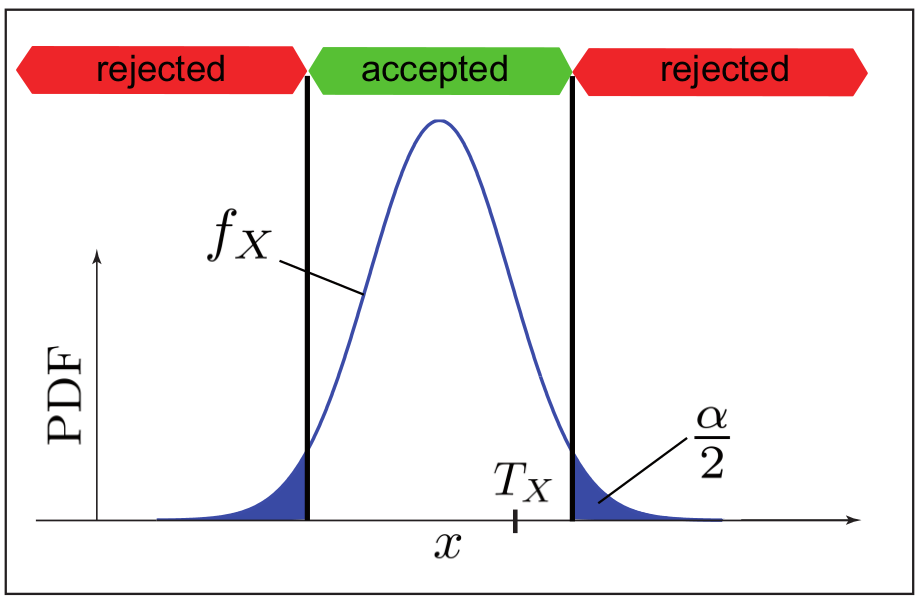
\includegraphics[trim = 0mm 0mm 0mm 2mm, clip, width=0.6\textwidth]{figures/SebastianNotesScreenshots/Screenshot2020-02-21t15-00-11.png}
	\caption{Hypothesis test}
	\label{Fig:HypTest}
\end{figure}

The significance level $\alpha = 1 - \text{Confidence}$, where $\text{Confidence}$ is the confidence value provided by the user, is typically equal to 0.95 or 0.99 (95\% or 99\%). For example, if the user specifies a 99\% confidence level, $\alpha = 0.01$. 

The most common PDF employed in a standard hypothesis test is the classic Gaussian (i.e. normal) distribution, for which regions of acceptance (i.e. $H_0$ is declared true) are:
\begin{itemize}
	\item $\approx \pm 1.96$ for $\alpha = 0.05$ (95\% confidence)
	\item $\approx \pm 2.58$ for $\alpha = 0.01$ (99\% confidence)
	\item $\approx \pm 3.29$ for $\alpha = 0.001$ (99.9\% confidence)
\end{itemize}
Ghilani \cite{ghilani} states ``In practice, authors have reported that a value of 3.29 also works as a criterion for rejection of blunders.'' 

However, the use of the Gaussian distribution is applicable only when the possible values for the standard residuals can extend infinitely in the positive or negative direction. When the a priori variance of unit weight, which describes how the least squares weighting matrix and the inverse of the measurement noise covariance are related (and thus is typically equal to identity), is used in lieu of the APV in equations \ref{eq:TestMetricStdRes} and \ref{eq:StdResVect}, as described in Ghilani \cite{ghilani} and Leick \cite{leick}, the assumption of infinite tails for the standard residual is reasonable. But when the APV is used as described in equations \ref{eq:TestMetricStdRes} and \ref{eq:StdResVect}, a different distribution is needed: the tau distribution, as described in section \ref{sec:TauDist}.

\subsection{Tau distribution} \label{sec:TauDist}

Unlike the standard residual formulations provided in Ghilani \cite{ghilani} and Leick \cite{leick}, a different convention is employed in Vanicek \& Krakiwsky (Chapter 13) \cite{vanicek1982geodesy} and Deakin \cite{deakin2018tau}: the APV is employed in the standard residual, as described in equations \ref{eq:TestMetricStdRes} and \ref{eq:StdResVect}. As a result of employing the APV, the standard residuals have finite limits. To derive these limits, first the standard residual is reformatted:
\begin{equation}\label{eq:StdRes}
\begin{split}
R_{std,i} &= \frac{R_{rel,i}}{\sqrt{\text{APV} \cdot r_i}} \\
&= \frac{R_{rel,i}}{\sqrt{\frac{(\text{RMS}(\textbf{R}_{rel}))^2 N_{\text{obs}}}{N_{\text{DOF}}} \; r_i}} \\
&= \frac{R_{rel,i}}{\sqrt{\frac{(\sum_{j=1}^{m} R_{rel,j}^2/N_{\text{obs}}) N_{\text{obs}}}{N_{\text{DOF}}} \; r_i}} \\
&= \frac{R_{rel,i}}{\sqrt{\sum_{j=1}^{m} R_{rel,j}^2}} \frac{\sqrt{N_{\text{DOF}}}}{\sqrt{r_i}}
\end{split}
\end{equation}
As a particular relative residual $R_{rel,i}$ approaches infinity, the finite limit of the standard residual is revealed:
\begin{equation}\label{eq:StdResLimit}
R_{std,i} \rightarrow \pm \frac{\sqrt{N_{\text{DOF}}}}{\sqrt{r_i}} \;\; \text{as} \;\; R_{rel,i} \rightarrow \pm \infty
\end{equation}

Note that the standard residual formulation in equations \ref{eq:TestMetricStdRes} and \ref{eq:StdResVect} is also referred to as an ``internally studentized residual''. In this formulation, the APV value is computed using all post-fit observation residuals, including any potential outliers. Because any anomalous residuals are included in the computation of the APV, which is in turn used to ``studentize'' or ``standardize'' the residuals, as a particular observation residual approaches infinity, the corresponding standard residual approaches the finite limit shown in equation \ref{eq:StdResLimit}. An alternative formulation is the ``externally studentized residual'', in which the APV does \textbf{not} include potential outliers. This formulation can have infinite limits as a result, but is not widely used.

When a scenario has non-infinite DOF, which is true for any adjustment performed in SALSA, alternatives to the Gaussian distribution are more representative of the relevant PDFs. One commonly used alternative is Student's t-distribution. However, the t-distribution has infinite tails, unlike the standard residual formulation in equations \ref{eq:TestMetricStdRes} and \ref{eq:StdResVect}. Thus a different alternative is employed: the tau distribution, as described in Pope \cite{pope1976statistics}, and Thompson \cite{thompson1935criterion}, and as illustrated in figure \ref{Fig:TauDist}.
\begin{figure} [!htb]
	\centering
	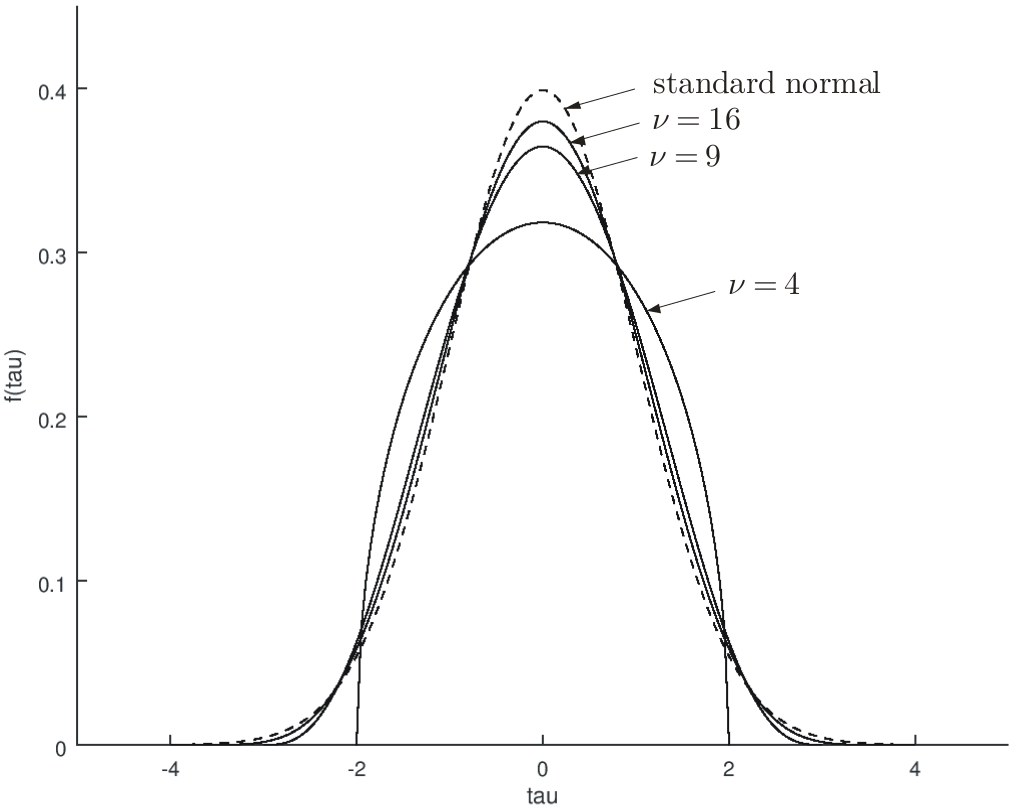
\includegraphics[trim = 0mm 0mm 0mm 0mm, clip, width=0.63\textwidth]{figures/DeakinScreenshots/TauDistributionCurves.png}
	% TwoSidedTest.png
	% Trim option parameter order: left bottom right top
	\caption{Tau distribution for different DOF ($\nu$)}
	\label{Fig:TauDist}
\end{figure}

Note how in figure \ref{Fig:TauDist} the tau distribution with DOF $\nu = 4$ has finite limits of $\pm 2$, and as the number of DOF increases, the tau distribution approaches the normal distribution (like the t-distribution). 

The tau distribution is closely tied to the t-distribution:
\begin{equation}\label{eq:TauEqn}
\tau_{\nu} = \frac{t_{\nu-1} \sqrt{\nu}}{\sqrt{\nu - 1 + t_{\nu-1}^2}}
\end{equation}
where $t_{\nu-1}$ is the t-distribution with $\nu - 1$ DOF.

If the value of $t$ within equation \ref{eq:TauEqn} approaches infinity, the finite limit of the tau distribution is revealed (suppressing subscripts):
\begin{equation}\label{eq:TauLimits}
\lim_{t \to \pm\infty} \tau = \lim_{t \to \pm\infty} \frac{t \sqrt{\nu}}{\sqrt{\nu - 1 + t^2}} = \sqrt{\nu} \lim_{t \to \pm\infty} \frac{t}{\sqrt{\nu - 1 + t^2}} = \pm \sqrt{\nu}
\end{equation}

To summarize, because the standard residual formulation provided in equations \ref{eq:TestMetricStdRes} and \ref{eq:StdResVect} has non-infinite limits, the tau distribution is the most appropriate distribution to use when computing thresholds for hypothesis testing: if the probability of standard residual values beyond those finite limits is zero, the PDF employed should reflect that reality. This reality also implies that if the a priori variance of unit weight (typically identity) is employed rather than the APV when computing standard residuals, a distribution with infinite tails such as the normal or t-distribution is more appropriate. 

Readers may note that the finite limits in equations \ref{eq:StdResLimit} and \ref{eq:TauLimits} are not identical: the standard residuals are bounded by $\pm \frac{\sqrt{\nu}}{\sqrt{r_i}}$, while the tau distribution is bounded by $\pm \sqrt{\nu}$. Section \ref{sec:ComputeThreshold} details how the tau distribution is scaled by $\frac{1}{\sqrt{r_i}}$ to appropriately account for the finite limits of the standard residuals. 

\subsection{Computing Threshold Values For Tau Distribution} \label{sec:ComputeThreshold}

To compute the hypothesis test threshold value using the tau distribution, first a confidence interval value must be specified. The value employed within SALSA is 95\%, or 0.95, which corresponds to a significance level $\alpha = 0.05$. If a larger confidence value is employed, the threshold values become larger, and thus fewer standard residuals will fail the statistical test.

SALSA employs a ``two-sided'' hypothesis test: the 5\% rejection region includes the area under the PDF curve for both sides of the distribution, as depicted in figure \ref{Fig:HypTest}. Because the tau distribution is symmetric, the area under the PDF curve for the right-side tail is $\alpha/2 = 0.025$. And because the shape of the PDF depends on the DOF $\nu$, as depicted in figure \ref{Fig:TauDist}, the x-axis boundaries of the rejection regions depend on the DOF $\nu$. 

The x-axis boundary value for the right-side tail, which is the hypothesis test threshold magnitude value of interest and is also referred to as the ``critical value'', has a CDF of $1-0.025 = 0.975$. (The cumulative distribution function, CDF, is the area under the PDF from negative infinity to a specified critical value.) Thus an ``inverse CDF'' function is needed: given the particular CDF of $0.975$, the inverse CDF function obtains the x-axis value corresponding to that CDF. 

The relationship between the tau distribution and the t-distribution (equation \ref{eq:TauEqn}) allows the use of the GPSTk t-distribution inverse CDF function \textit{invStudentsCDF} to compute the tau distribution threshold:
\begin{equation}\label{eq:InvCDF}
\begin{split}
t_{\nu-1} &= \text{\textit{invStudentsCDF}}(1-\alpha/2,\nu-1) \\
\tau_{\nu} &= t_{\nu-1} \cdot \sqrt{\nu} / \sqrt{\nu-1+t_{\nu-1}^2} \\
\text{Test Threshold} &= \tau_{\nu} / \sqrt{r_i}
\end{split}	
\end{equation}

The method provided in equation \ref{eq:InvCDF} works for all scenarios with DOF equal to 2 or greater. When the DOF equals 0 (exactly determined system with no redundancy) or 1 (only a single degree of freedom for the entire survey), the standard residual threshold is not computed. However, scenarios with DOF equal to 0 or 1 are unlikely to occur for real-world surveys (though they might occur for simple toy problems set up for analysis and troubleshooting).

\section{Internal Reliability}

Internal reliability, also known as the minimum detectable bias for a particular observation, is based on two confidence (probability) threshold values, the measurement uncertainty, and the redundancy (local reliability) metric. The two threshold values are:

\begin{itemize}
	\item $\alpha$ = Probability the observation is considered a blunder, when it is actually not
	\item $\beta$ = Probability the observation is not considered a blunder, when it actually is
\end{itemize}

\begin{figure}[!htb]
	\centering
	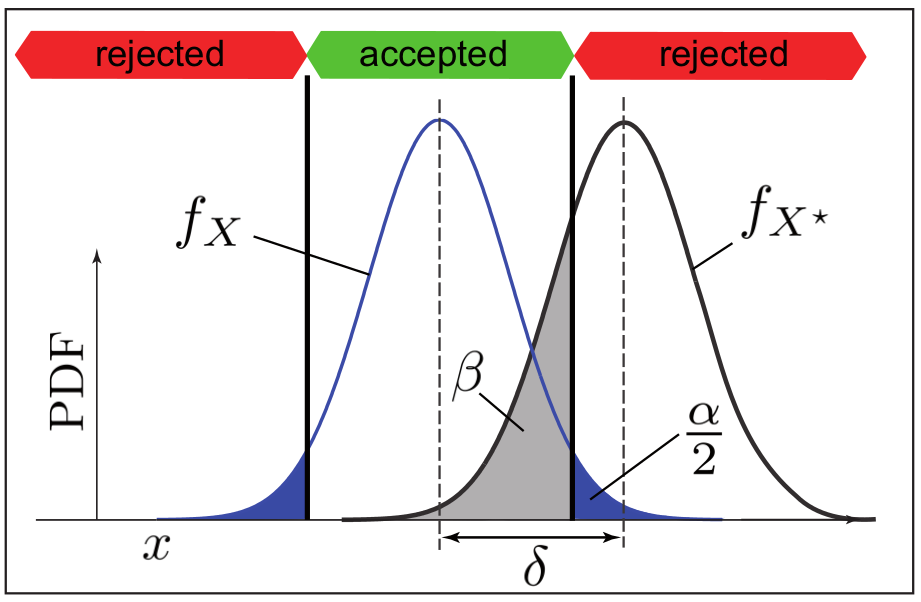
\includegraphics[trim = 0mm 0mm 0mm 2mm, clip, width=0.6\textwidth]{figures/SebastianNotesScreenshots/Screenshot2020-02-21t14-58-49.png} 
	\caption{Relationship between $\alpha$, $\beta$, and $\delta$}
	\label{Fig:AlphaaBetaDelta}
\end{figure}

Common values are $\alpha = 0.01$ and $\beta = 0.05$. Figure B.3 provides a visual representation of the ``no blunder'' (i.e. null) and ``blunder'' hypotheses. Both hypotheses are assumed to have Gaussian (i.e. standard, or normal) distribution, and the blunder hypothesis has a non-zero mean value. That non-zero mean value, also equal to the distance between the center of each distribution, is referred to as the ``non-centrality parameter'' $\delta_0$. For $\alpha = 0.01$ and $\beta = 0.05$, the non-centrality parameter is $\delta_0 = 4.22068$. 

To compute the minimum detectable bias, the minimum gross error $\nabla Y_i$ is set equal to the gross error $\Delta \hat{Y}_i$ which produces a test statistic $T_N$ equal to $\delta_0$:
\begin{equation}\label{eq:MinDetectBlunder1}
T_N = \Delta \hat{Y}_i / \sigma_{\Delta \hat{Y}_i} = \delta_0
\end{equation}

However, instead of setting $\sigma_{\Delta \hat{Y}_i}$ equal to the expression for $\sigma_{\Delta Y_i}$ provided by equation \ref{eq:SigmaY} to derive the final expression for $T_N$, a slightly different expression is used:
\begin{equation}\label{eq:SigmaYv2}
\sigma_{\Delta \hat{Y}_i} = \frac{\text{MCov}_{ii}}{\sqrt{Q_{RR,ii}}}
\end{equation}
where the $\sqrt{\text{APV}}$ term has been removed. Why is $\sqrt{\text{APV}}$ not employed? Leick \cite{leick} provides an explanation: ``Baarda’s (1967) development of the concept of reliability of networks is based on un-Studentized hypothesis tests, which means that the a priori variance of unit weight is assumed to be known. Consequently, the a priori variance of unit weight (not the a posteriori variance of unit weight) is used in this section.'' The a priori variance of unit weight is assumed equal to identity, and thus the expression is simplified to the form in equation \ref{eq:SigmaYv2}. A significant benefit of this revision is that the internal reliability metric (and thus the external reliability metric as defined in section \ref{sec:ExtRel}) for each observation is not dependent on any actual observations collected in the field, and thus can serve as a powerful planning tool prior to the survey.

The minimum detectable bias is then computed as:
\begin{equation}\label{eq:MinDetectBlunder2}
\begin{split}
\nabla \hat{Y_i} &= \delta_0 \; \sigma_{\Delta \hat{Y}_i} \\
&= \delta_0 \; \frac{\text{MCov}_{ii}}{\sqrt{Q_{RR_{ii}}}} \\
&= \delta_0 \; \frac{\text{MCov}_{ii}}{\sqrt{Q_{RR_{ii}}}} \frac{Q_{RR_{ii}}}{\text{MCov}_{ii}} \frac{1}{r_i} \\
&= \delta_0 \; \frac{\sqrt{Q_{RR_{ii}}}}{r_i}\\
&= \delta_0 \; \frac{\sqrt{r_i \; \text{MCov}_{ii}}}{r_i}\\
&= \delta_0 \; \frac{\sqrt{\text{MCov}_{ii}}}{\sqrt{r_i}}
\end{split}
\end{equation}

For a given $\delta_0$ and $\text{MCov}_{ii}$, a larger redundancy number means a smaller minimum detectable bias. In other words, the minimum detectable bias is inversely proportional to the square root of the individual redundancy value. An observation with low redundancy and thus a large minimum detectable bias can potentially significantly derail the estimated state (i.e. adjusted position), as illustrated in section \ref{sec:RelExamples}.

\section{External Reliability} \label{sec:ExtRel}

External reliability is calculated by mapping the minimum detectable blunders for each observation through the state update operation, which provides the impact on the estimated state from that blunder:

\begin{equation}\label{eq:MapMinDetBlunderToState}
\nabla \hat{\textbf{x}}_i = \left( H^T \; \text{MCov}^{-1} \; H \right)^{-1} H^T \; \text{MCov}^{-1} \; \nabla \hat{\textbf{Y}}_i
\end{equation}

where $\nabla \hat{\textbf{Y}}_i$ is a vector of m elements which are all equal to zero except the $i^{\text{th}}$ element, which has value $\nabla \hat{Y}_i$:

\begin{equation}\label{eq:eq:MapMinDetBlunderToState3}
\nabla \hat{\textbf{Y}}_i = \begin{bmatrix}
0 & \ldots & 0 & \nabla \hat{Y}_i & 0 & \ldots & 0
\end{bmatrix}^T
\end{equation}

The result is an array of ``state impact'' vectors, one for each observation. Lower redundancy leads to a larger minimum detectable bias, which in turn leads to larger state impact vectors. 

To visualize these state impact vectors, a ''Reliability Rectangle'' is constructed, as illustrated in figure \ref{Fig:RR}. This rectangle allows the user to quickly grasp the effect that strong or weak redundancy in the observations has on the final state. The result is intuitive and actionable information for the surveyor regarding the susceptibility of any planned or collected observations to blunders or significant outliers.

A reliability rectangle is defined by the following properties:
\begin{itemize}
    \item The rectangle is centered at the estimated state position (or the a priori position if the survey has not yet been conducted)
    \item All external reliability vectors are rotated into the ENU frame, using the above center position as the reference position for that rotation
    \item The rectangle is oriented such that the major axis direction matches the direction of the largest magnitude state vector, and the scaling of the rectangle in that direction matches the magnitude of the largest magnitude state vector
    \item The smaller dimension of the rectangle is scaled to fit all the other external reliability vectors
\end{itemize}

\begin{figure}[!htb]
	\centering
	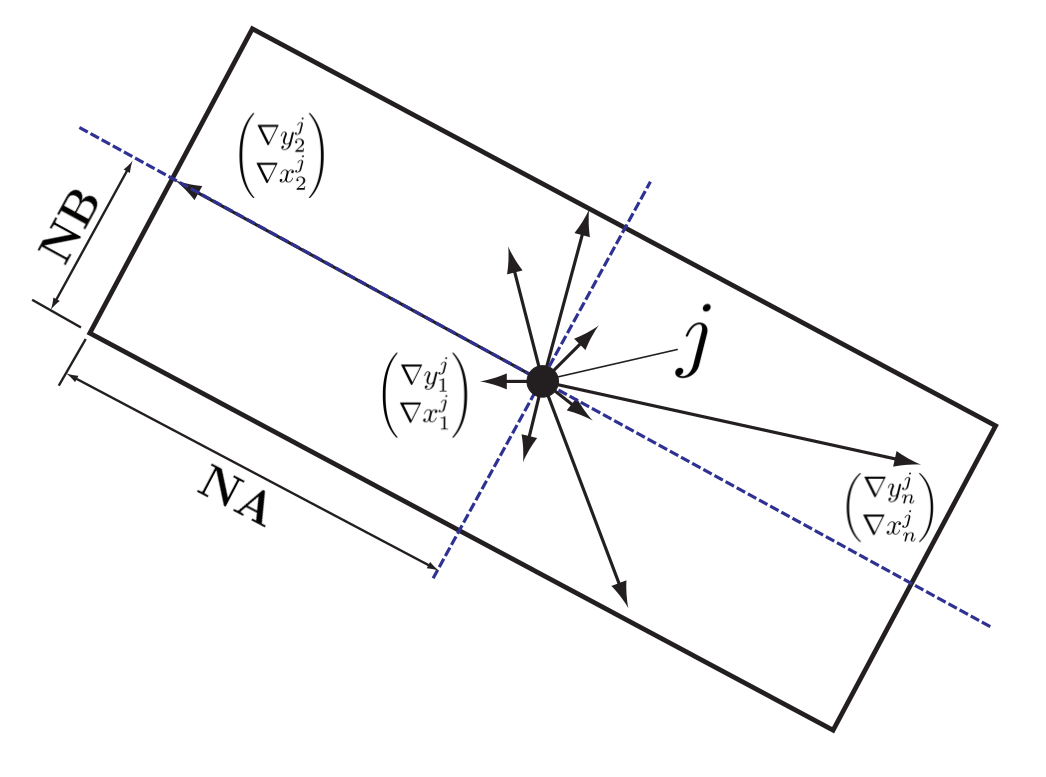
\includegraphics[trim = 0mm 0mm 0mm 2mm, clip, width=0.8\textwidth]{figures/SebastianNotesScreenshots/Screenshot2020-02-24t09-52-28.png} 
	\caption{Example reliability rectangle}
    \label{Fig:RR}
\end{figure}

\newpage

\section{Examples} \label{sec:RelExamples}

Below are two ``toy problems'' that illustrate the utility of the above metrics for surveyors. While a typical survey has many more observations than these simple examples, employing relatively few  observations in these examples hopefully allows the reader to more easily grasp the nature of the reliability metrics and how they are computed for each observation.

\subsection{Range Example}

The first simple example employs range observations from several stations to estimate a desired position, as illustrated by figure \ref{Fig:Ex1Map}. Note that the example contains no specific distance units. The position of interest is located at [0,10], with the true position matching the a priori nominal position to simplify the example. The ranging station positions are fixed at [0,0], [1,0], and [10,10]. Measurement noise of 0.01 1-$\sigma$ is added to the observations, and a measurement uncertainty of 0.01 1-$\sigma$ is employed in the estimation process (and thus all measurements have equal weight).

\newpage

\begin{figure}[!htb] 
	\centering
	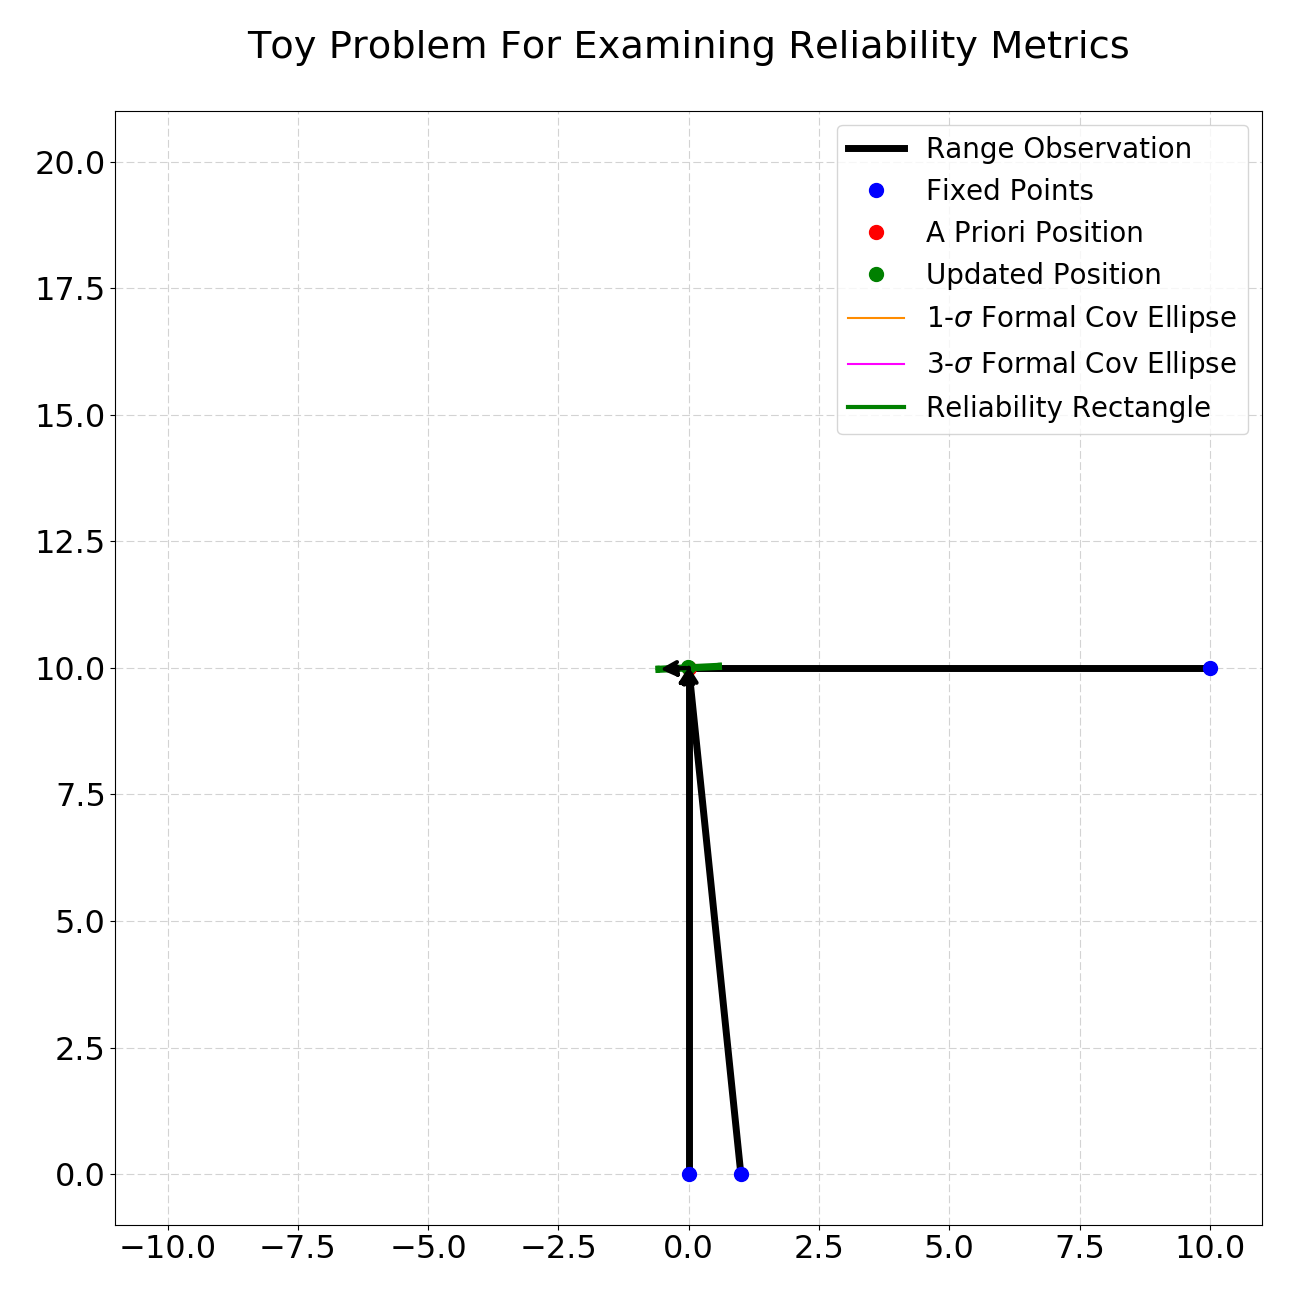
\includegraphics[trim = 0mm 0mm 0mm 5mm, clip, width=0.9\textwidth]{figures/ReliabilityExample/v10/Map.png}
	\caption{Ranging example - map}
    \label{Fig:Ex1Map}
\end{figure}

\newpage

Figure \ref{Fig:Ex1MapZoom} provides a zoomed-in view of the region around the point of interest. The formal uncertainty is visible via the 3-$\sigma$ formal covariance ellipse, which appears reasonably sized in both directions. In contract, the magnitude of the reliability rectangle is large in the East-West direction - far larger than the formal covariance scaling in the East-West direction. The lack of redundancy in the East-West direction from having only one ranging station to the East of the estimated position results in a large reliability rectangle magnitude.

\begin{figure}[!htb]
	\centering
	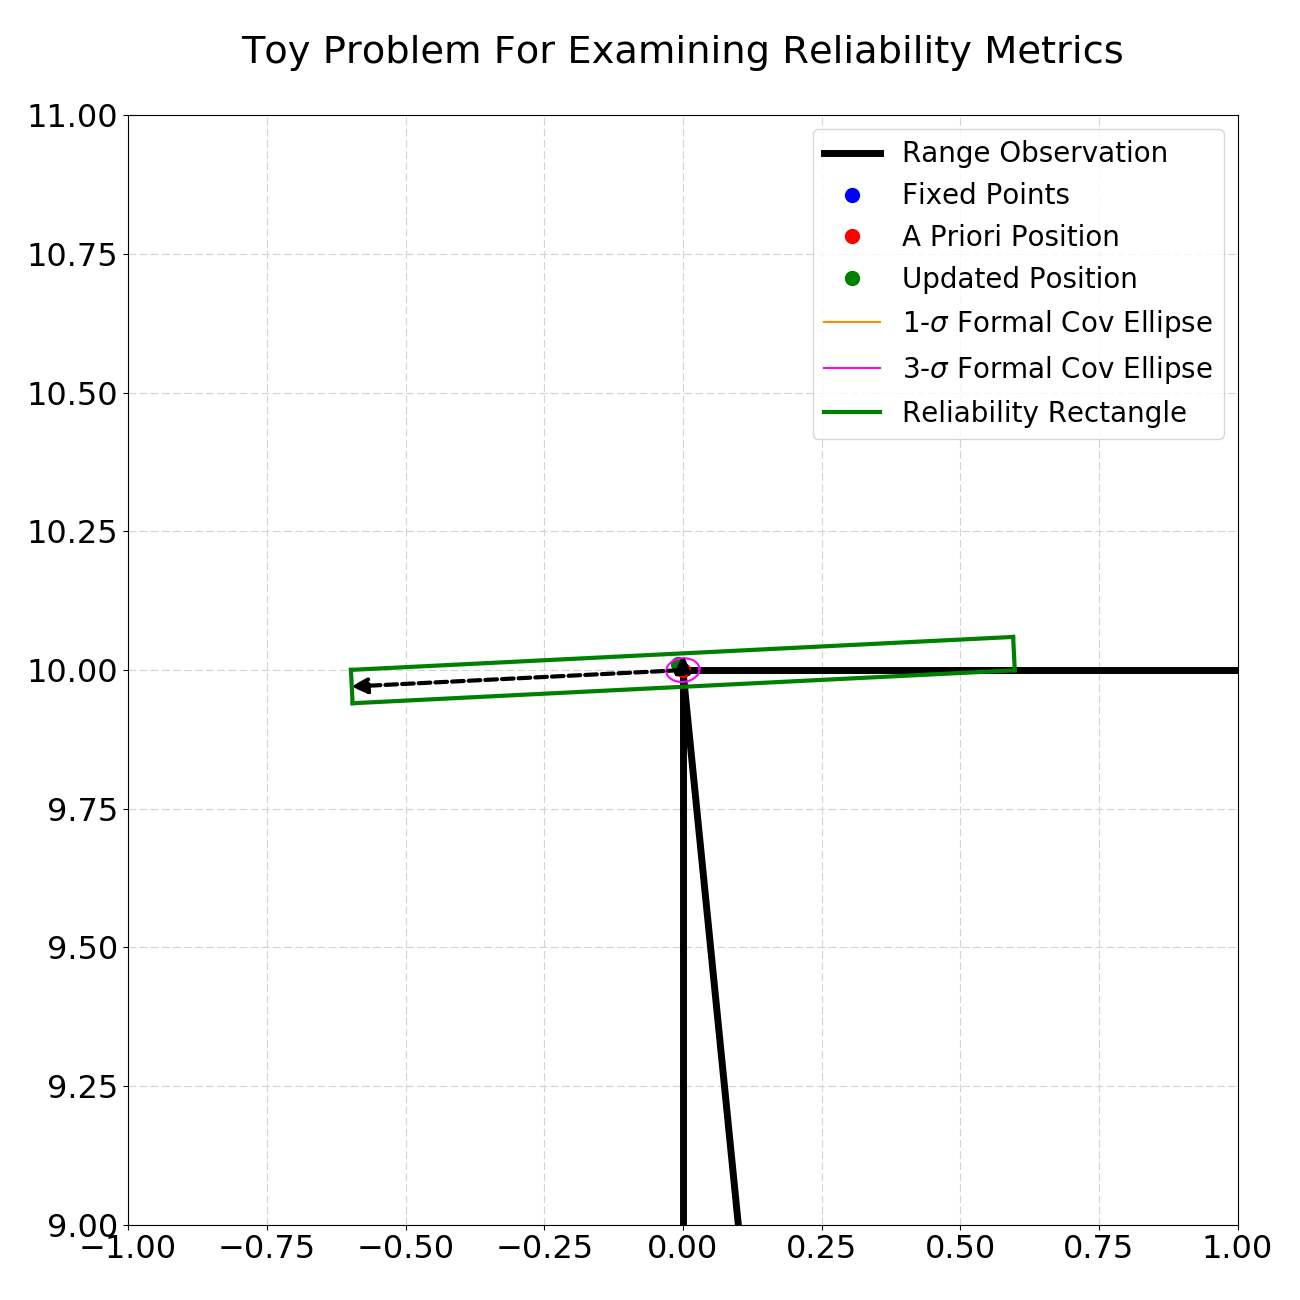
\includegraphics[trim = 0mm 0mm 0mm 5mm, clip, width=0.9\textwidth]{figures/ReliabilityExample/v10/MapZoomed.png}
	\caption{Ranging example - zoomed map}
    \label{Fig:Ex1MapZoom}
\end{figure}

\newpage

To demonstrate what a reliability rectangle illustrates, the minimum detectable bias computed for the East station range observation is added to that observation, as shown in figure \ref{Fig:Ex1MapZoomBlunder}. The result: the estimated position now lies approximately on the western edge of the reliability rectangle. (The estimated position lands exactly on the edge if no measurement noise is added.)

\begin{figure}[!htb]
	\centering
	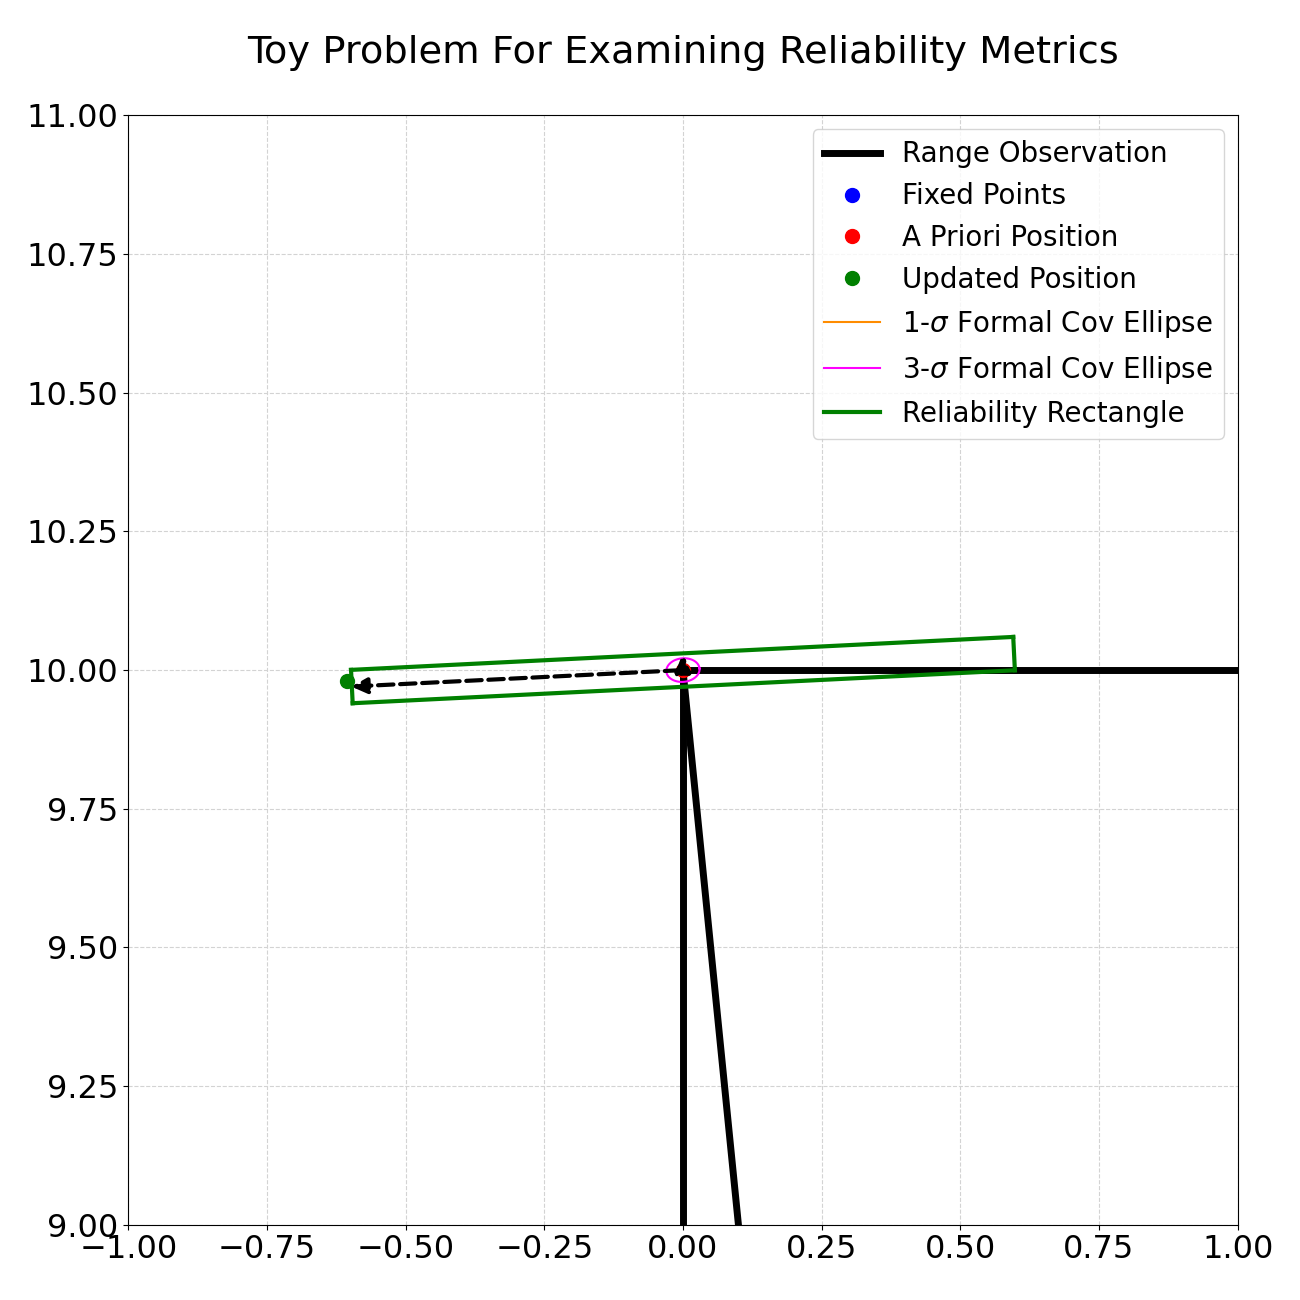
\includegraphics[trim = 0mm 0mm 0mm 5mm, clip, width=0.9\textwidth]{figures/ReliabilityExample/v13/MapZoomed.png}
	\caption{Ranging example - east station blunder}
    \label{Fig:Ex1MapZoomBlunder}
\end{figure}

\newpage

To illustrate how the estimated position is so heavily affected by a blunder in a low redundancy observation, each of the ranging observations can be viewed as a circle with radius equal to the range value, as shown in figure \ref{Fig:Ex1MapObs}:

\begin{figure}[!htb]
    \centering
    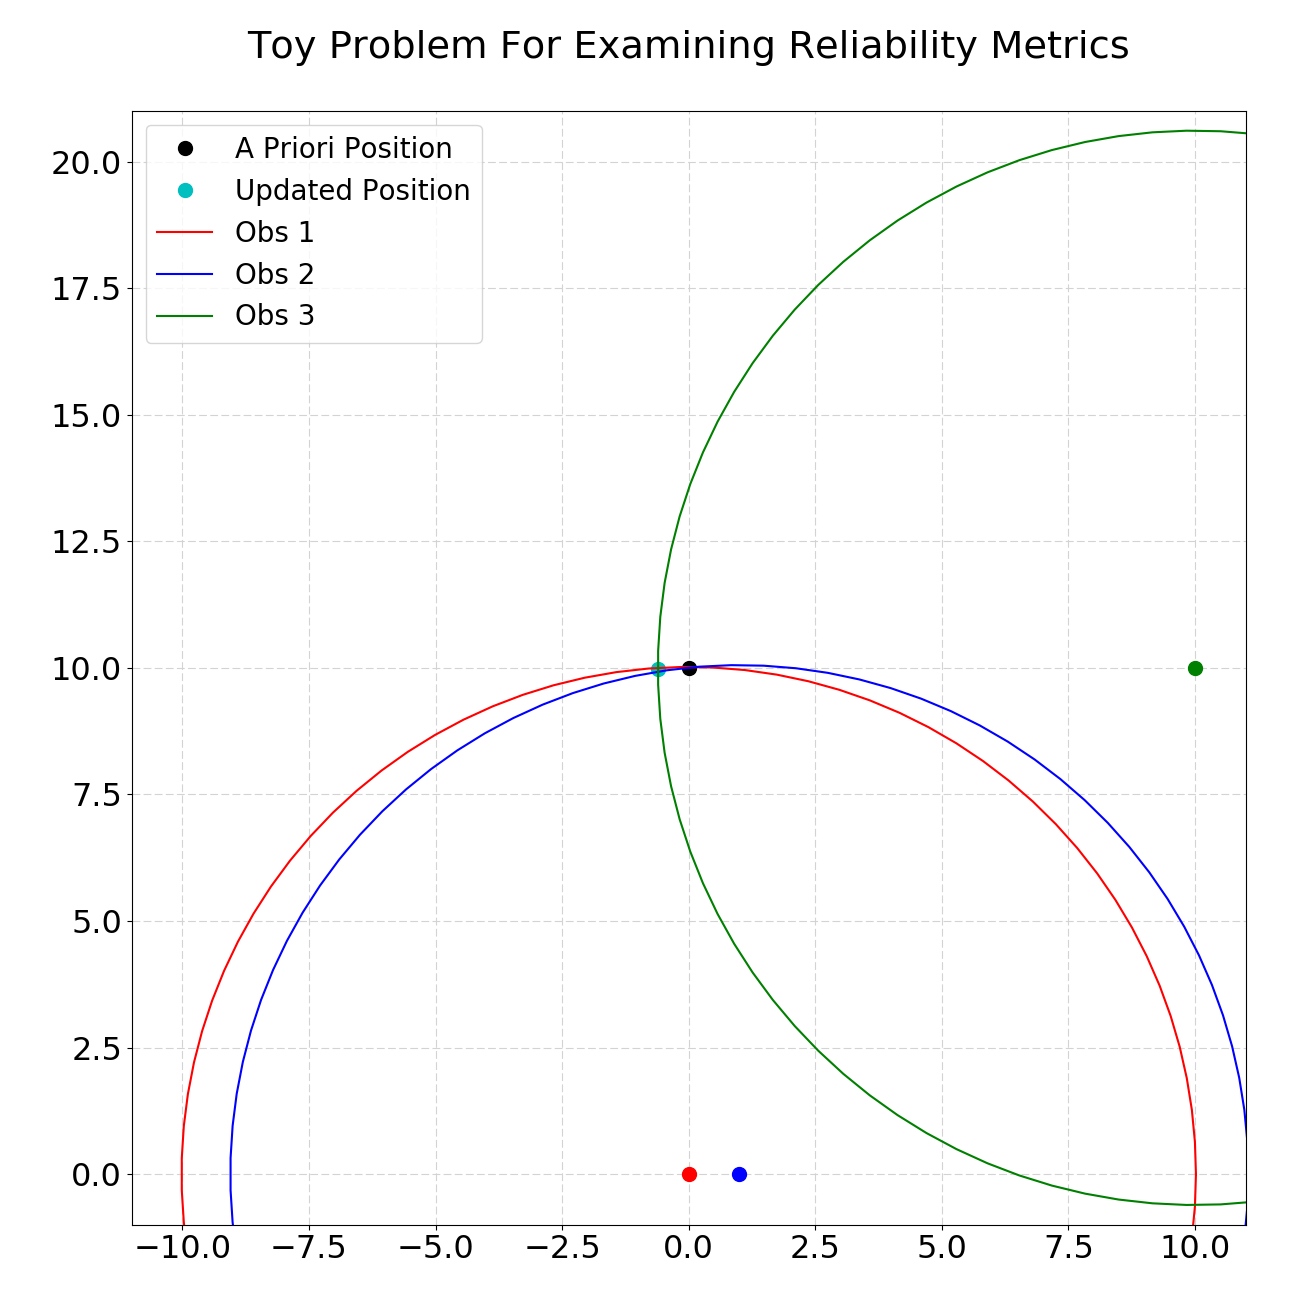
\includegraphics[trim = 0mm 0mm 0mm 0mm, clip, width=1.0\textwidth]{figures/ReliabilityExample/v53/MapObs.png}
    \caption{Ranging example - observations as circles}
    \label{Fig:Ex1MapObs}
\end{figure}


\newpage

Zooming in on the point of interest, figure \ref{Fig:Ex1MapObsZoomed} shows the estimated position is now 0.6 units to the west, just as in figure \ref{Fig:Ex1MapZoomBlunder}. The least squares estimation process identifies the position that minimizes the sum of the squared pre-fit residuals, which means the estimated position lies on the ``Obs 3'' line between the ``Obs 1'' and ``Obs 2'' lines - the best place to minimize those residuals. The low redundancy of the east station observation allows this large blunder to significantly affect the state.

\begin{figure}[!htb]
    \centering
    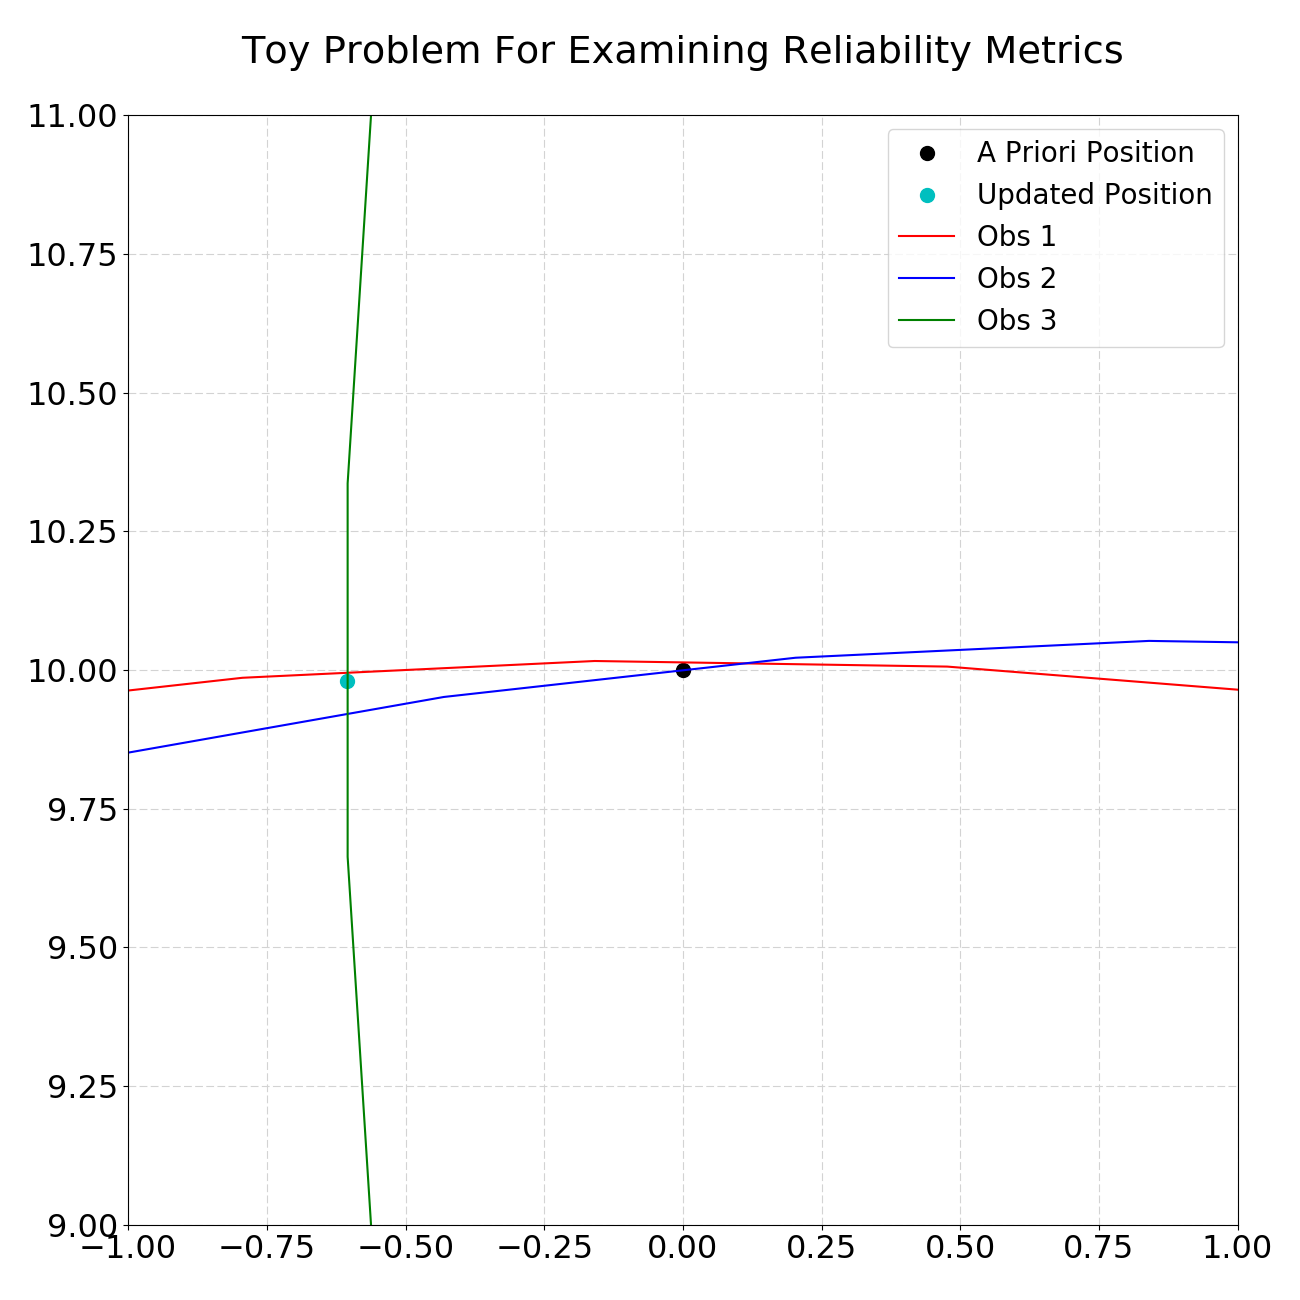
\includegraphics[trim = 0mm 0mm 0mm 0mm, clip, width=1.0\textwidth]{figures/ReliabilityExample/v53/MapObsZoomed.png}
    \caption{Ranging example - observations as circles}
    \label{Fig:Ex1MapObsZoomed}
\end{figure}

%MapObsZoomed.png


 
\newpage

The pre-fit and post-fit observation residuals for the blunder scenario are provided in figures \ref{Fig:Ex1PrefitRes} and \ref{Fig:Ex1PostfitRes}. Note that while the third pre-fit residual (corresponding to the East station range observation) is clearly the largest residual, the third post-fit residual is reasonably close to zero and smaller than the other two residuals. Thus an analysis of the post-fit residuals can easily miss any blunders or outliers in observations that have poor redundancy, and these blunders or outliers can also lead to the rejection of good observations if the surveyor does not address this lack of redundancy (e.g. throwing out observation two in this scenario, as it has the largest magnitude post-fit residual).

%\newpage
\begin{figure}[!htb]
	\centering
	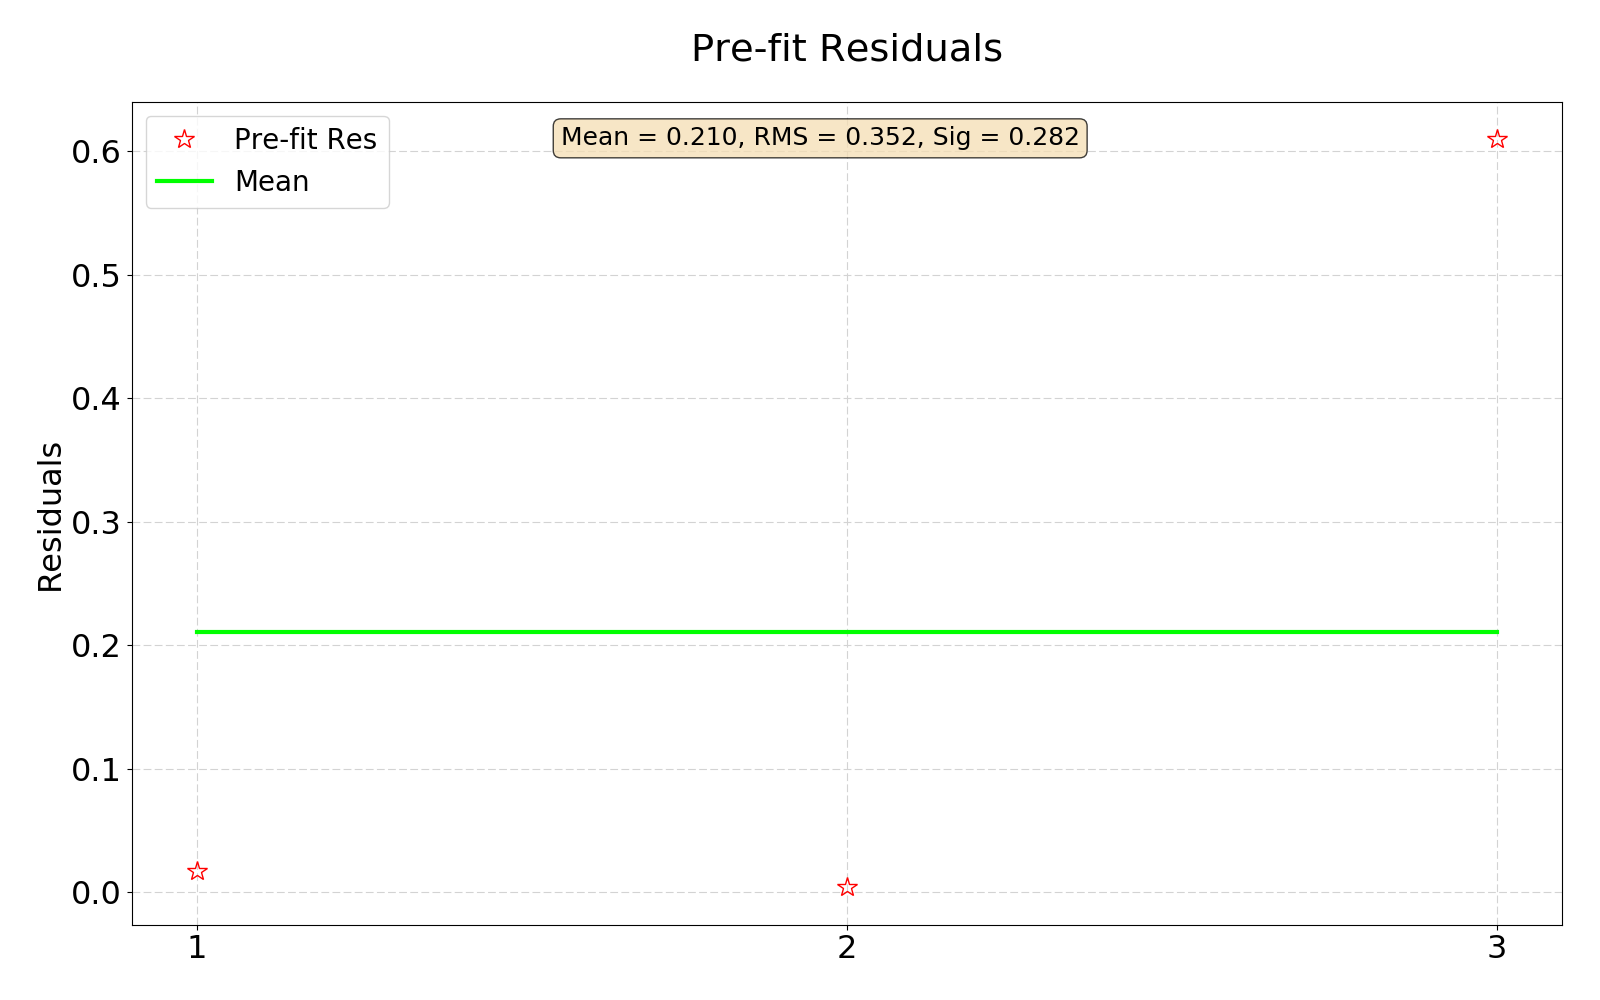
\includegraphics[trim = 0mm 0mm 0mm 0mm, clip, width=1.0\textwidth]{figures/ReliabilityExample/v53/PrefitResiduals.png}
	\caption{Ranging example - east station blunder pre-fit residuals}
    \label{Fig:Ex1PrefitRes}
\end{figure}

\newpage
\begin{figure}[!htb]
	\centering
	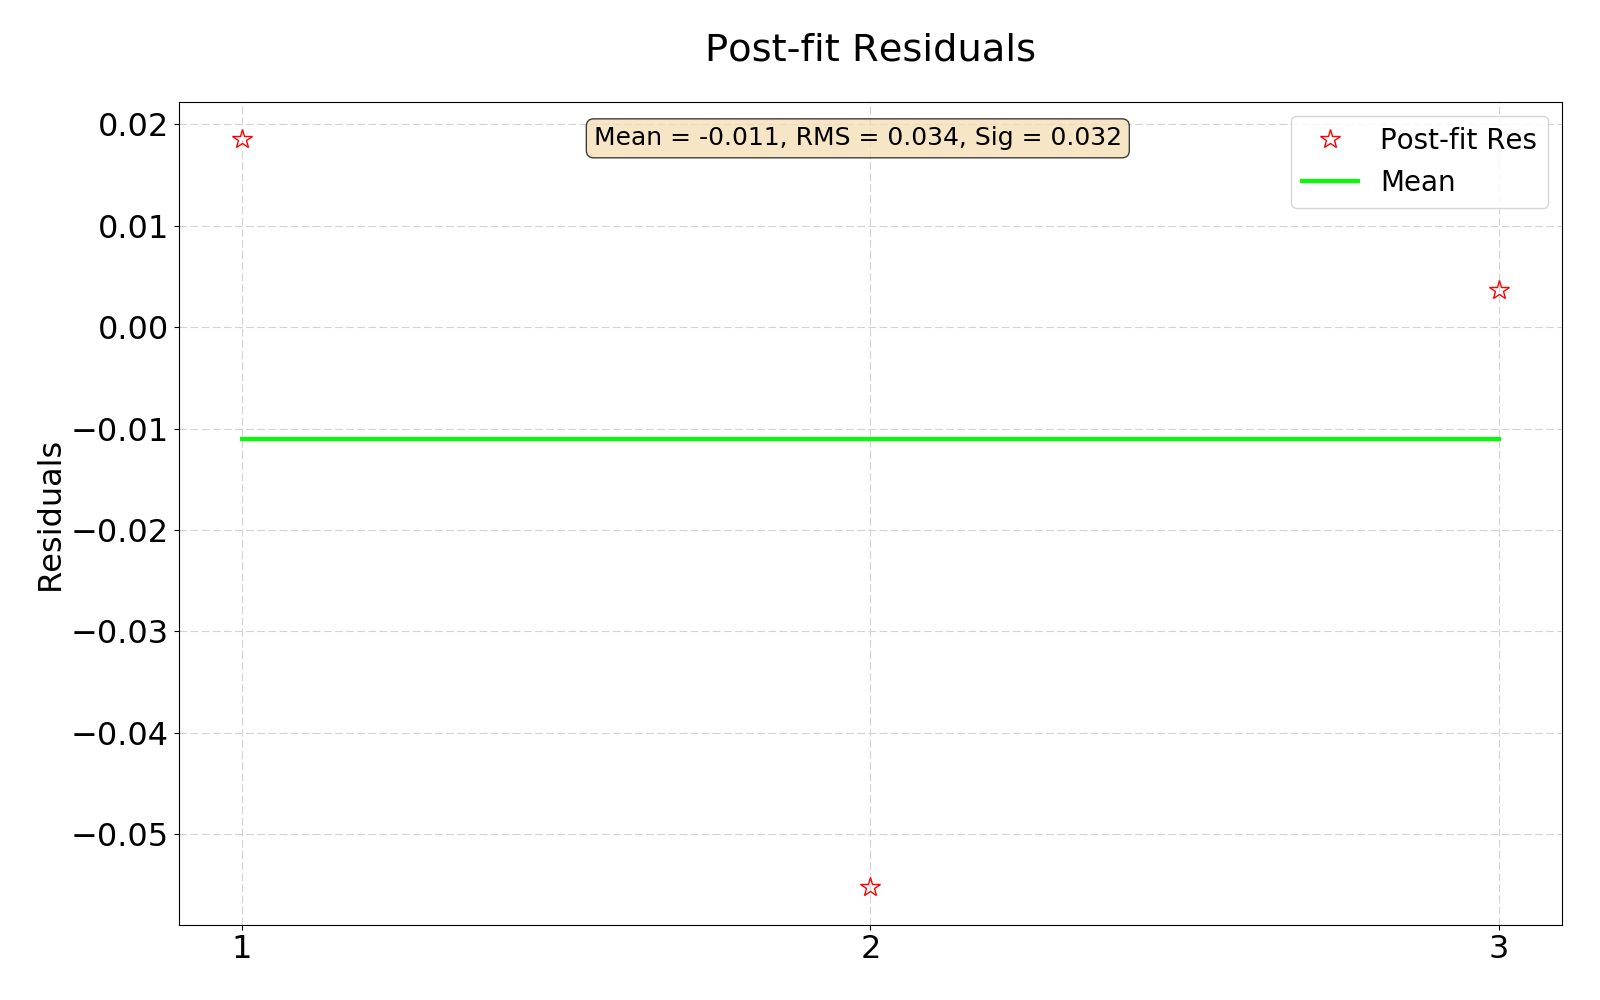
\includegraphics[trim = 0mm 0mm 0mm 0mm, clip, width=1.0\textwidth]{figures/ReliabilityExample/v53/PostfitResiduals.png}
	\caption{Ranging example - east station blunder post-fit residuals}
    \label{Fig:Ex1PostfitRes}
\end{figure}

\newpage

The redundancy values (local reliability) for the three observations highlight how the third observation has almost no redundancy, as shown in figure \ref{Fig:Ex1redundancy}.

\begin{figure}[!htb]
	\centering
	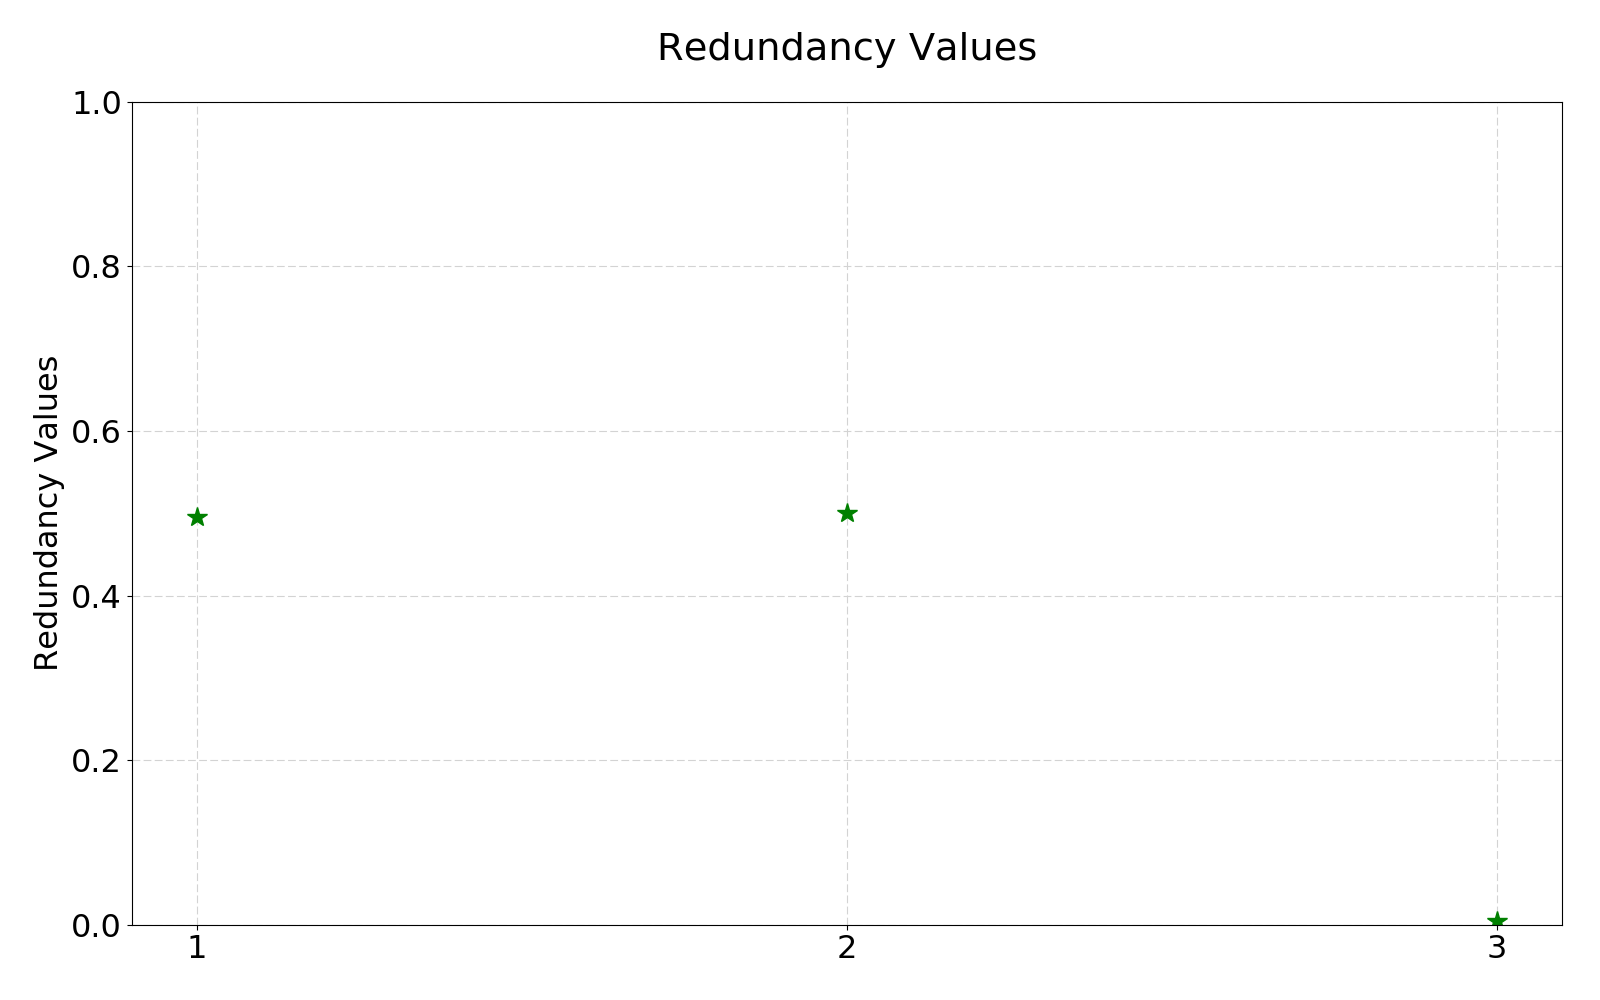
\includegraphics[trim = 0mm 0mm 0mm 0mm, clip, width=1.0\textwidth]{figures/ReliabilityExample/v53/Redundancy.png}
	\caption{Ranging example - redundancy values}
    \label{Fig:Ex1redundancy}
\end{figure}

\newpage

The minimum detectable bias values (internal reliability) for the three observations, as shown in figure \ref{Fig:Ex1minDetBias}, reveals how the third observation has a significantly larger magnitude due to the poor redundancy of that observation:

\begin{figure}[!htb]
	\centering
	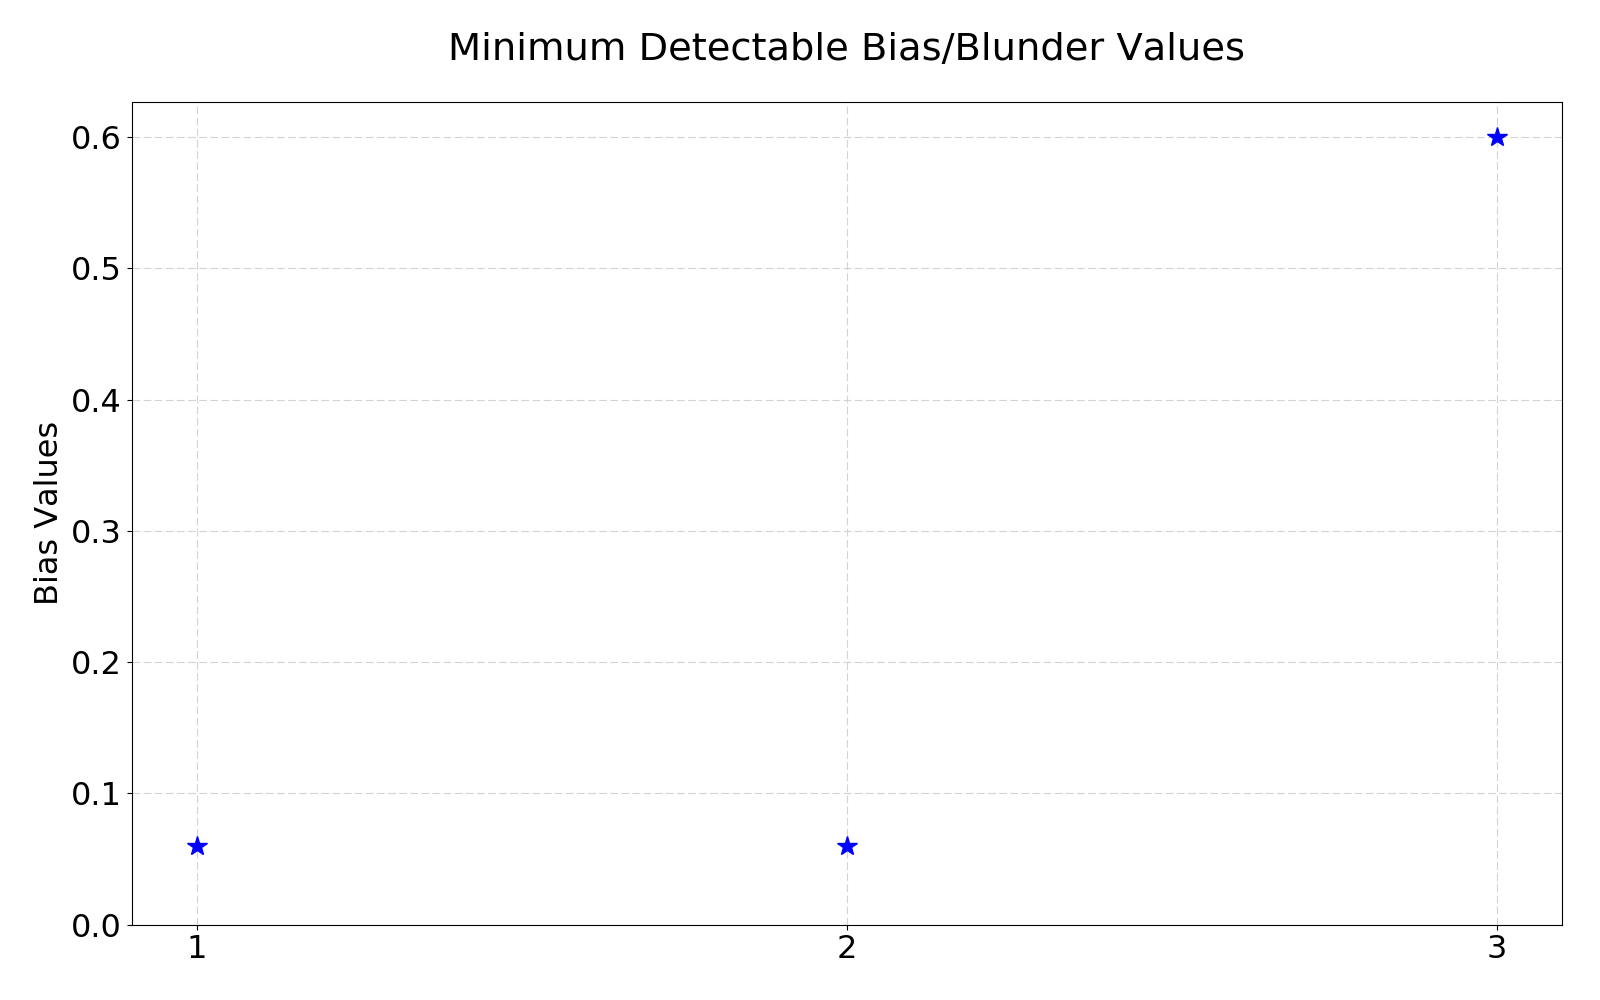
\includegraphics[trim = 0mm 0mm 0mm 0mm, clip, width=1.0\textwidth]{figures/ReliabilityExample/v53/MinDetBias.png}
	\caption{Ranging example - minimum detectable bias values}
    \label{Fig:Ex1minDetBias}
\end{figure}

\newpage

The external reliability vector magnitudes for the three observations, as shown in figure \ref{Fig:Ex1ExtVectMag}, similarly shows the third observation has a much larger magnitude than the other two observations:

\begin{figure}[!htb]
	\centering
	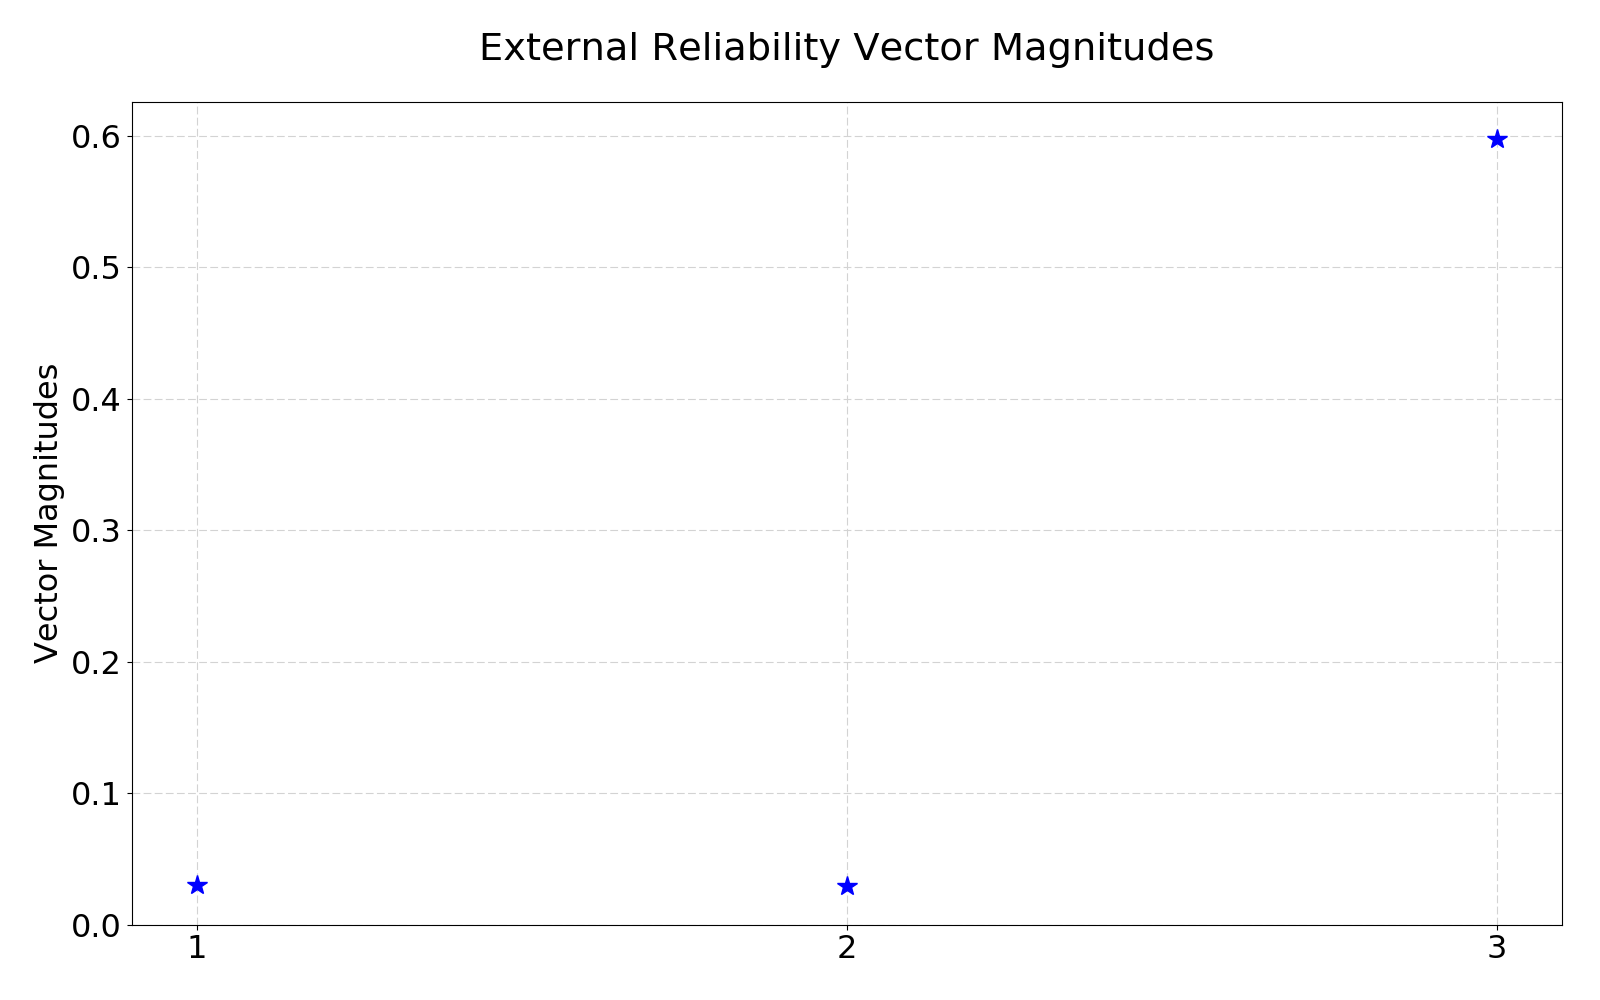
\includegraphics[trim = 0mm 0mm 0mm 0mm, clip, width=1.0\textwidth]{figures/ReliabilityExample/v53/ExtRelVectMags.png}
	\caption{Ranging example - external reliability vector magnitudes}
    \label{Fig:Ex1ExtVectMag}
\end{figure}

\newpage

The post-fit residuals plotted in figure \ref{Fig:Ex1PostfitRes} can be transformed into standard residuals, as described in section \ref{sect:StdRes}. The results are provided in figure \ref{Fig:Ex1StdRes}. Note that even though the observation 3 has the blunder, the largest standard residual magnitude occurs for observation 2. Thus if the surveyor only checks the standard residual magnitudes and ignores the redundancy, internal reliability, and external reliability metrics, a good observation can be excluded and a blunder can remain. In other words, standard residuals can prove unreliable in identifying blunders if sufficient redundancy is not established for all observations.

\begin{figure}[!htb]
	\centering
	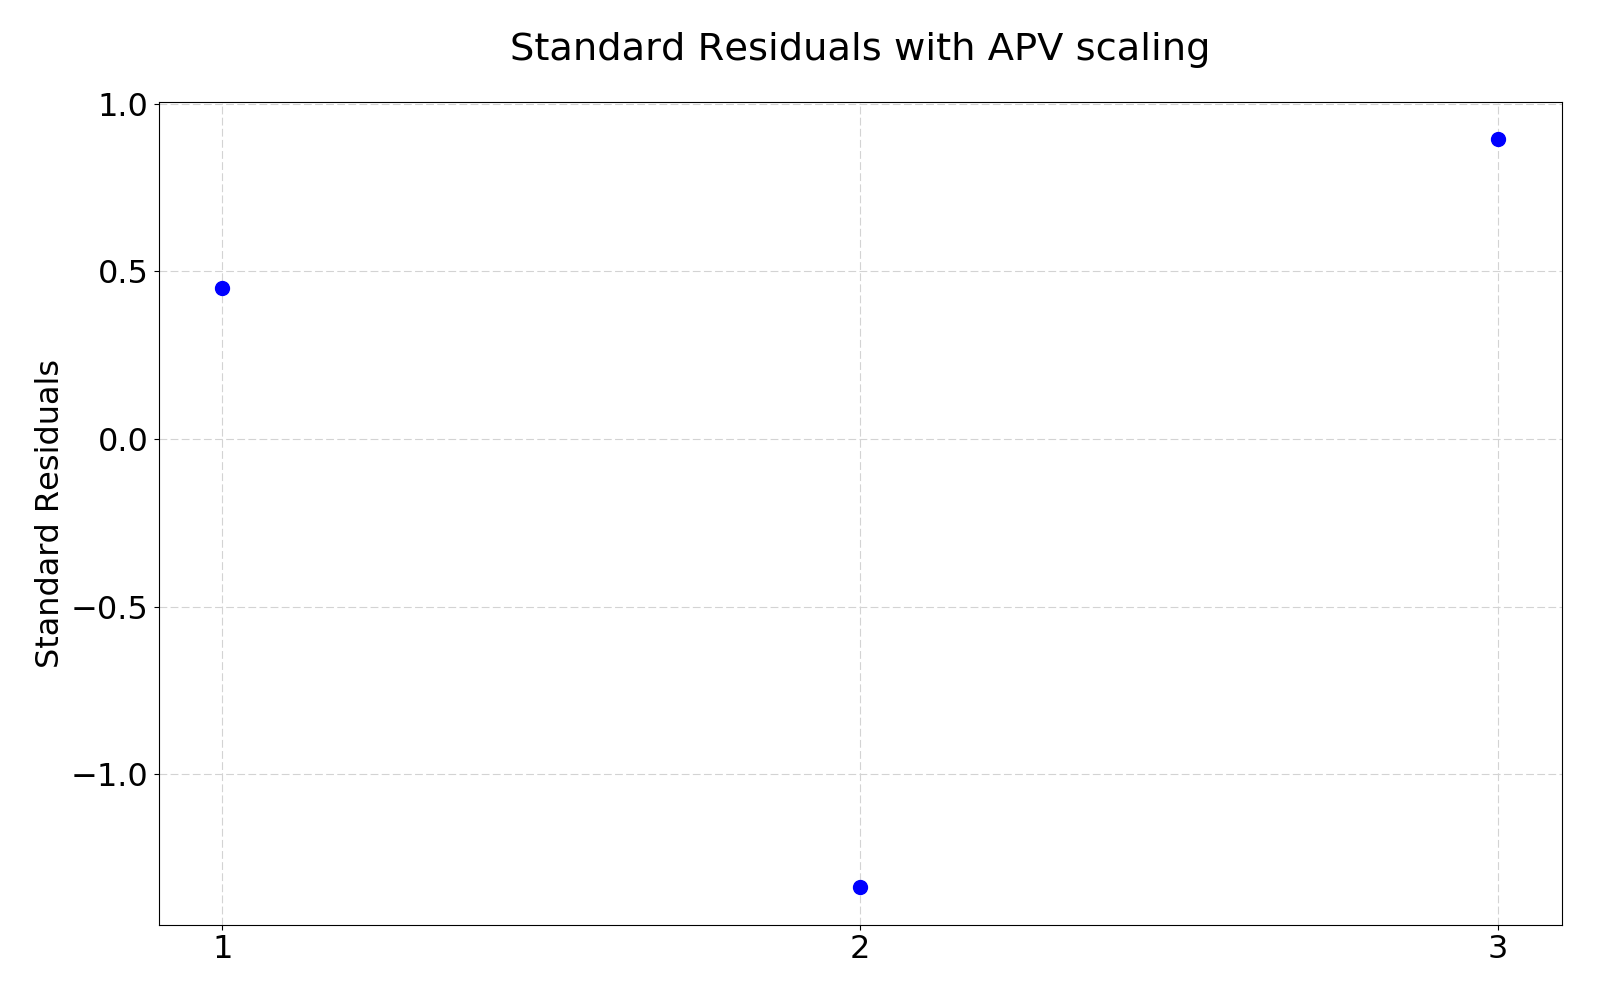
\includegraphics[trim = 0mm 0mm 0mm 0mm, clip, width=1.0\textwidth]{figures/ReliabilityExample/v54/StandardResidualsWithAPV.png}
	\caption{Ranging example - standard residuals with east station blunder}
    \label{Fig:Ex1StdRes}
\end{figure}

\newpage
Given the wide reliability rectangle presented in figure \ref{Fig:Ex1MapZoom}, a good course of action is to add observations that provide redundancy in the east-west direction. Figure \ref{Fig:Ex1AddedObsMap} illustrates the result of adding two ranging stations to the east (neither of which contain blunders, but the blunder for observation 3 remains):

\begin{figure}[!htb]
	\centering
	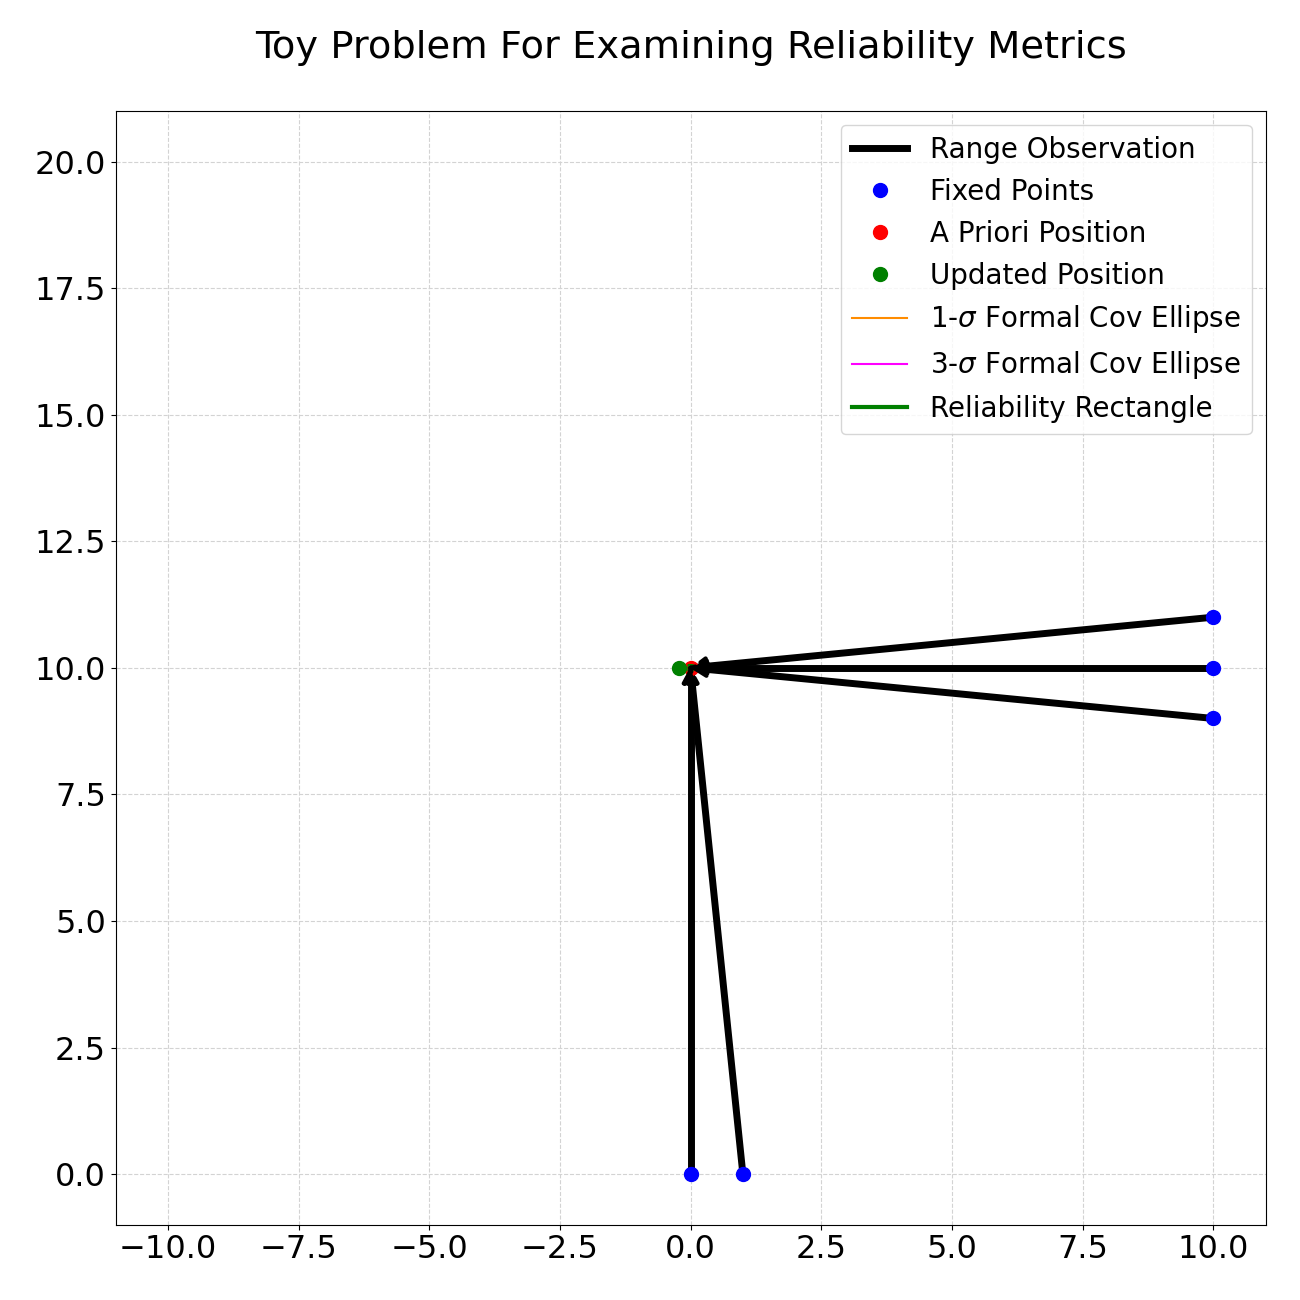
\includegraphics[trim = 0mm 0mm 0mm 5mm, clip, width=0.9\textwidth]{figures/ReliabilityExample/v15/Map.png}
	\caption{Ranging example - adding additional observations}
    \label{Fig:Ex1AddedObsMap}
\end{figure}

\newpage
Zooming in on the point of interest, figure \ref{Fig:Ex1AddedObsMapZoomed} shows the estimated position is approximately 0.2 units to the west, rather than 0.6 as seen in figure \ref{Fig:Ex1MapObsZoomed}. The positive influence of the additional measurements results in a smaller impact on the estimated state from the observation 3 blunder.

\begin{figure}[!htb]
	\centering
	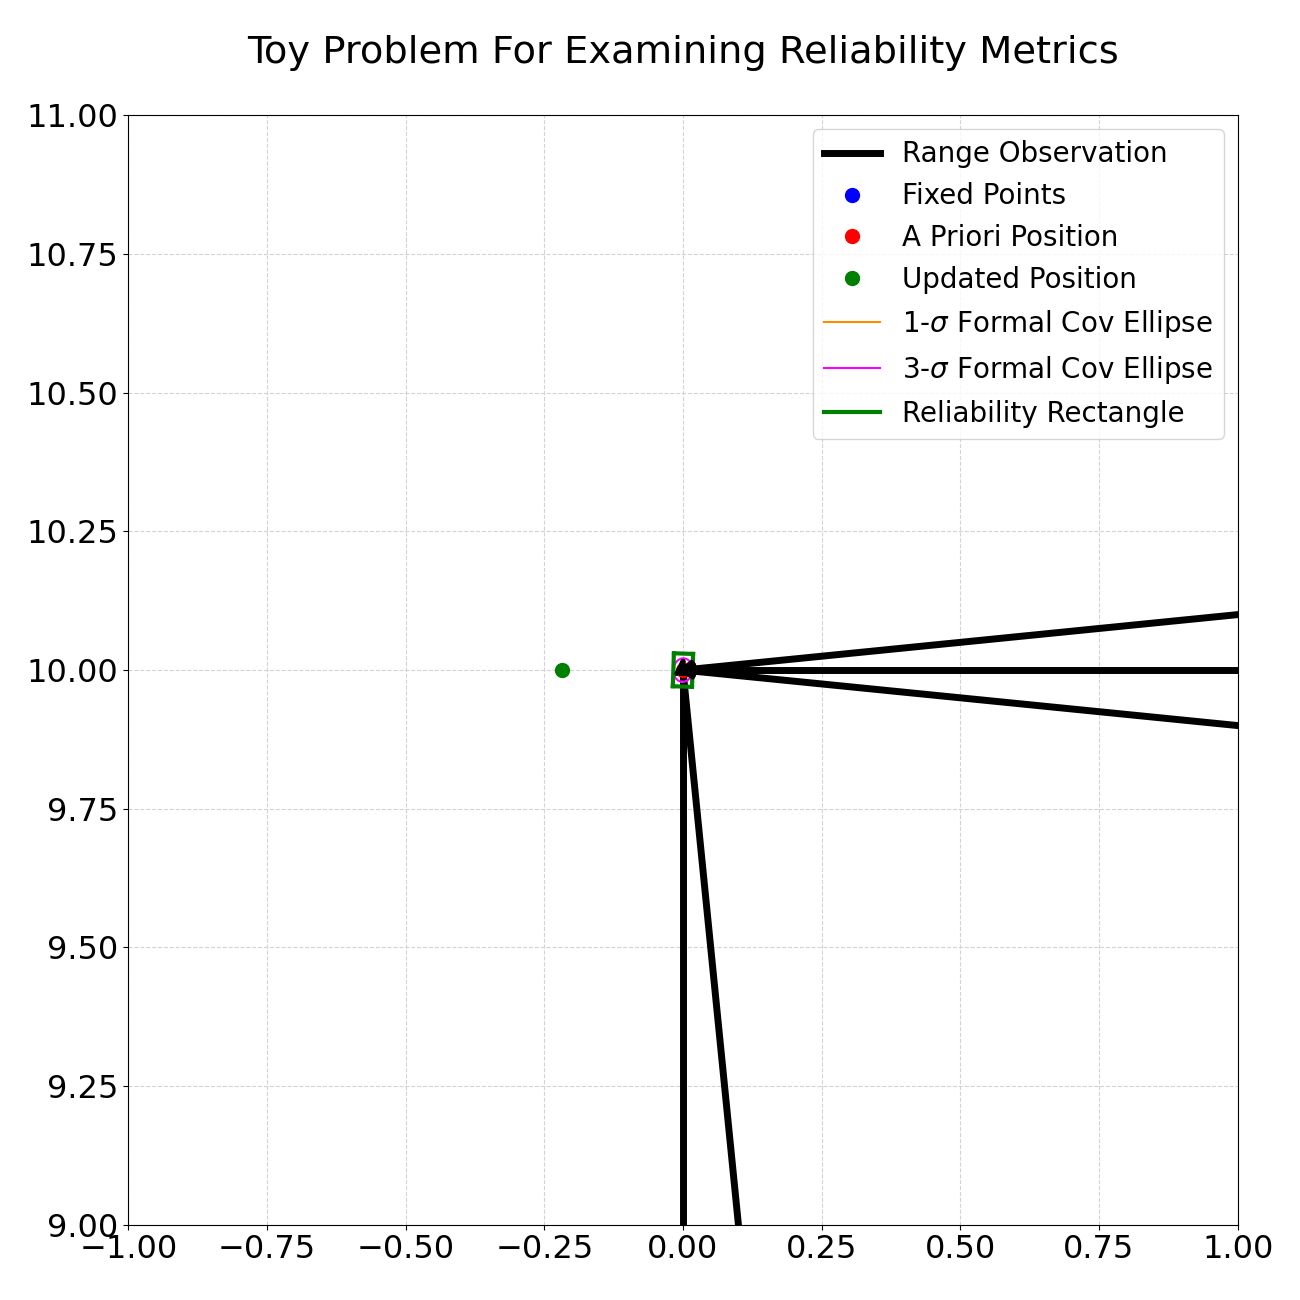
\includegraphics[trim = 0mm 0mm 0mm 5mm, clip, width=0.9\textwidth]{figures/ReliabilityExample/v15/MapZoomed.png}
	\caption{Ranging example - adding additional observations - zoomed}
    \label{Fig:Ex1AddedObsMapZoomed}
\end{figure}

\newpage

Now that all observations have reasonable redundancy, the standard residuals now correctly identify the blunderous observation, as shown in figure \ref{Fig:Ex1AddedObsStdRes}.

\begin{figure}[!htb]
	\centering
	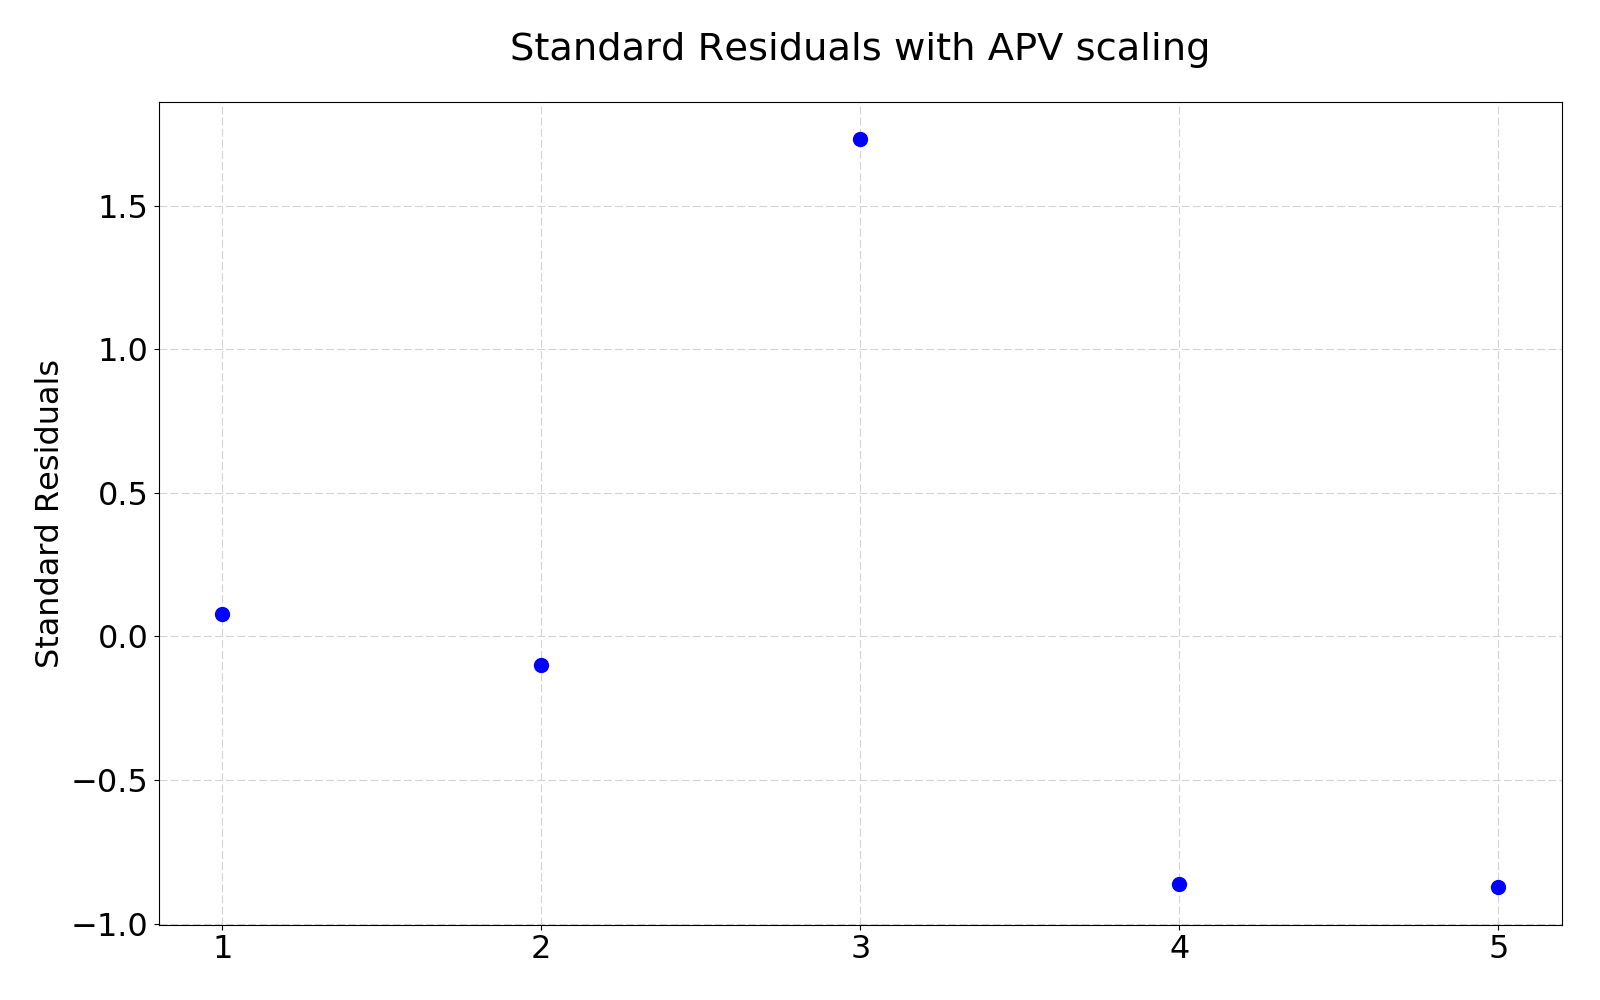
\includegraphics[trim = 0mm 0mm 0mm 0mm, clip, width=1.0\textwidth]{figures/ReliabilityExample/v55/StandardResidualsWithAPV.png}
	\caption{Ranging example - adding additional observations - standard residuals}
    \label{Fig:Ex1AddedObsStdRes}
\end{figure}

\subsection{Angles Example}

An analogous example to the ranges-only example involves only azimuth angle observations, as shown in figure \ref{Fig:Ex2Map}. As in the previous example, the position of interest is located at [0,10], measurement noise of 0.1$^{\circ}$ 1-$\sigma$ is employed, and the measurement uncertainty is also set as 0.1$^{\circ}$ 1-$\sigma$.

\newpage

\begin{figure}[!htb] 
    \centering
    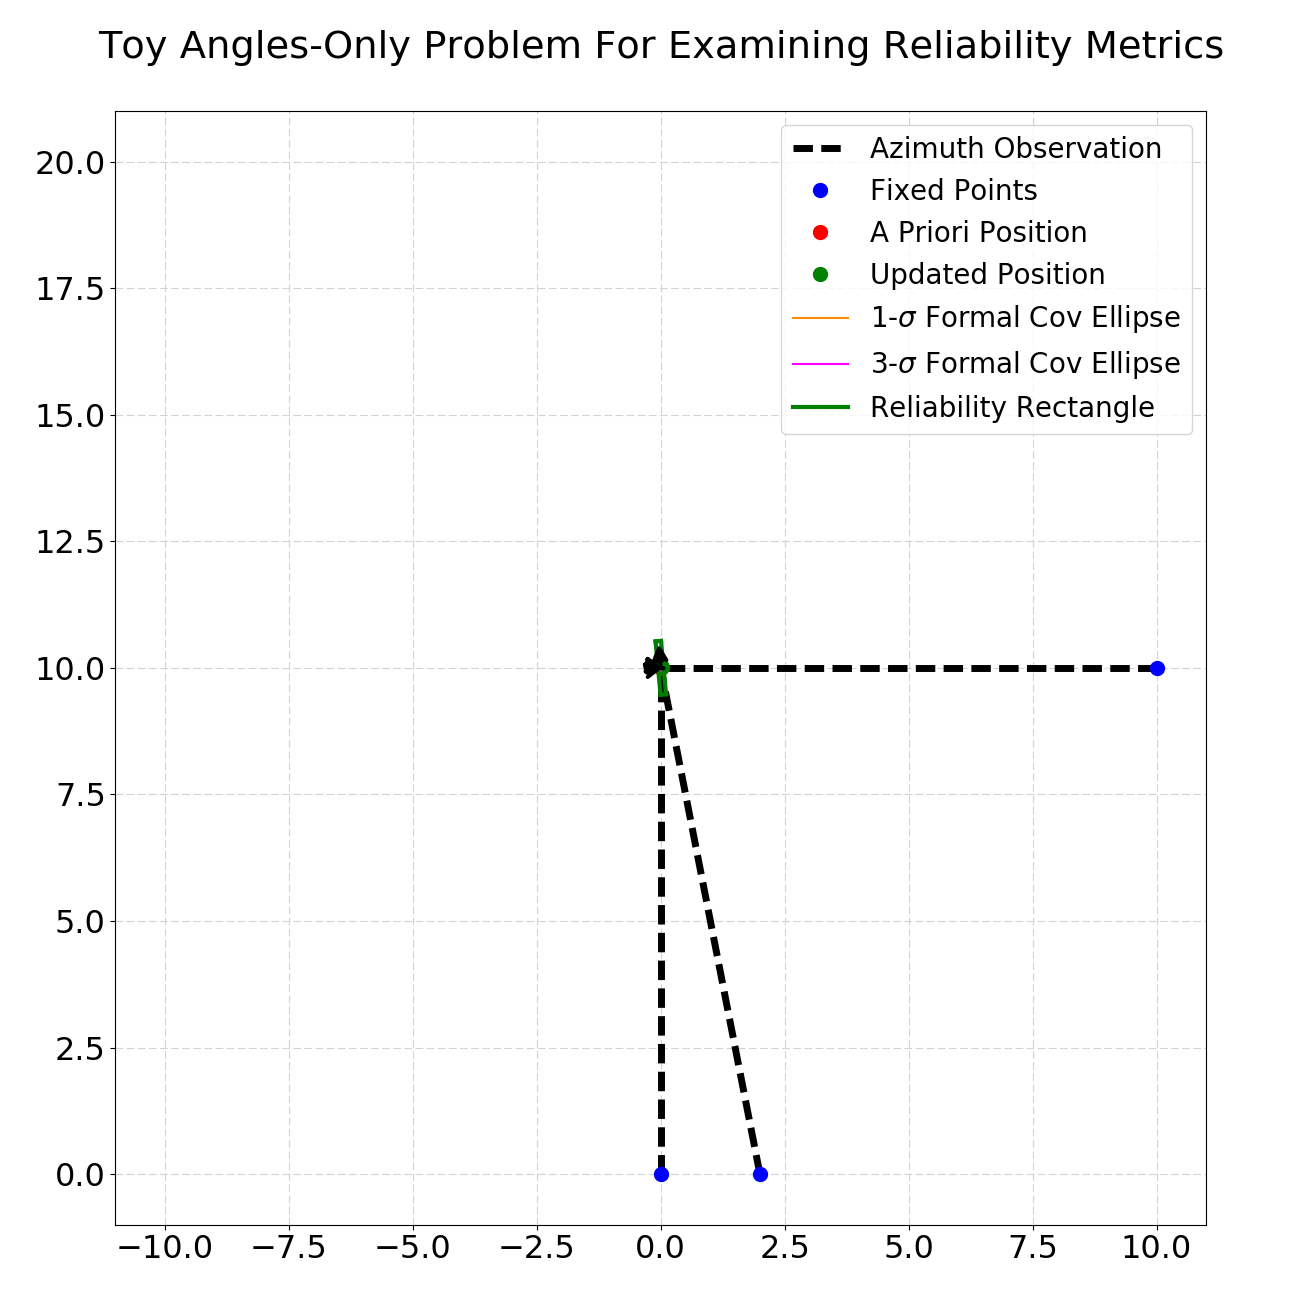
\includegraphics[trim = 0mm 0mm 0mm 5mm, clip, width=0.9\textwidth]{figures/ReliabilityExample/v22/Map.png}
    \caption{Angles example - map}
    \label{Fig:Ex2Map}
\end{figure}

\newpage

Figure \ref{Fig:Ex2MapZoom} provides a zoomed-in view of the region around the point of interest, with the formal uncertainty and reliability rectangle more visible. Unlike in Example 1, the reliability rectangle has large magnitude in the North-South axis due to lack of redundancy in that direction from having only one station to the East providing a direction observation.

\begin{figure}[!htb]
    \centering
    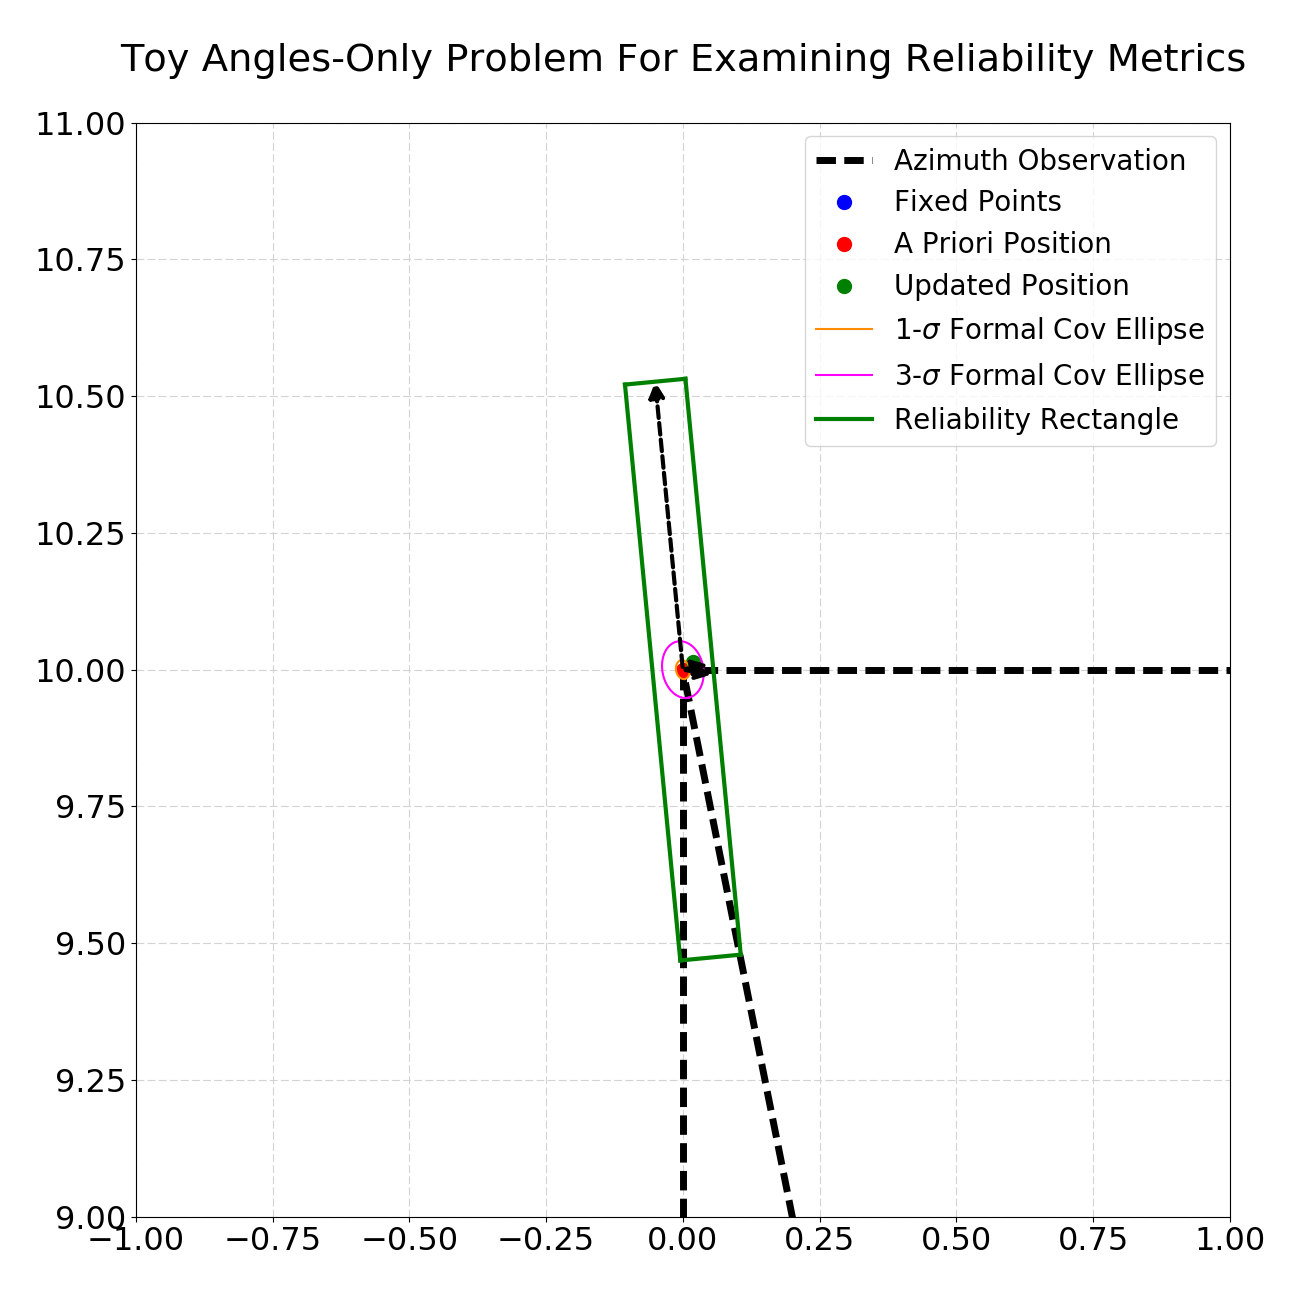
\includegraphics[trim = 0mm 0mm 0mm 5mm, clip, width=0.9\textwidth]{figures/ReliabilityExample/v22/MapZoomed.png}
    \caption{Angles example - zoomed map}
    \label{Fig:Ex2MapZoom}
\end{figure}

\newpage

The redundancy values (local reliability) for the three observations highlight how the third observation has almost no redundancy, as shown in figure \ref{Fig:Ex2redundancy}.

\begin{figure}[!htb]
    \centering
    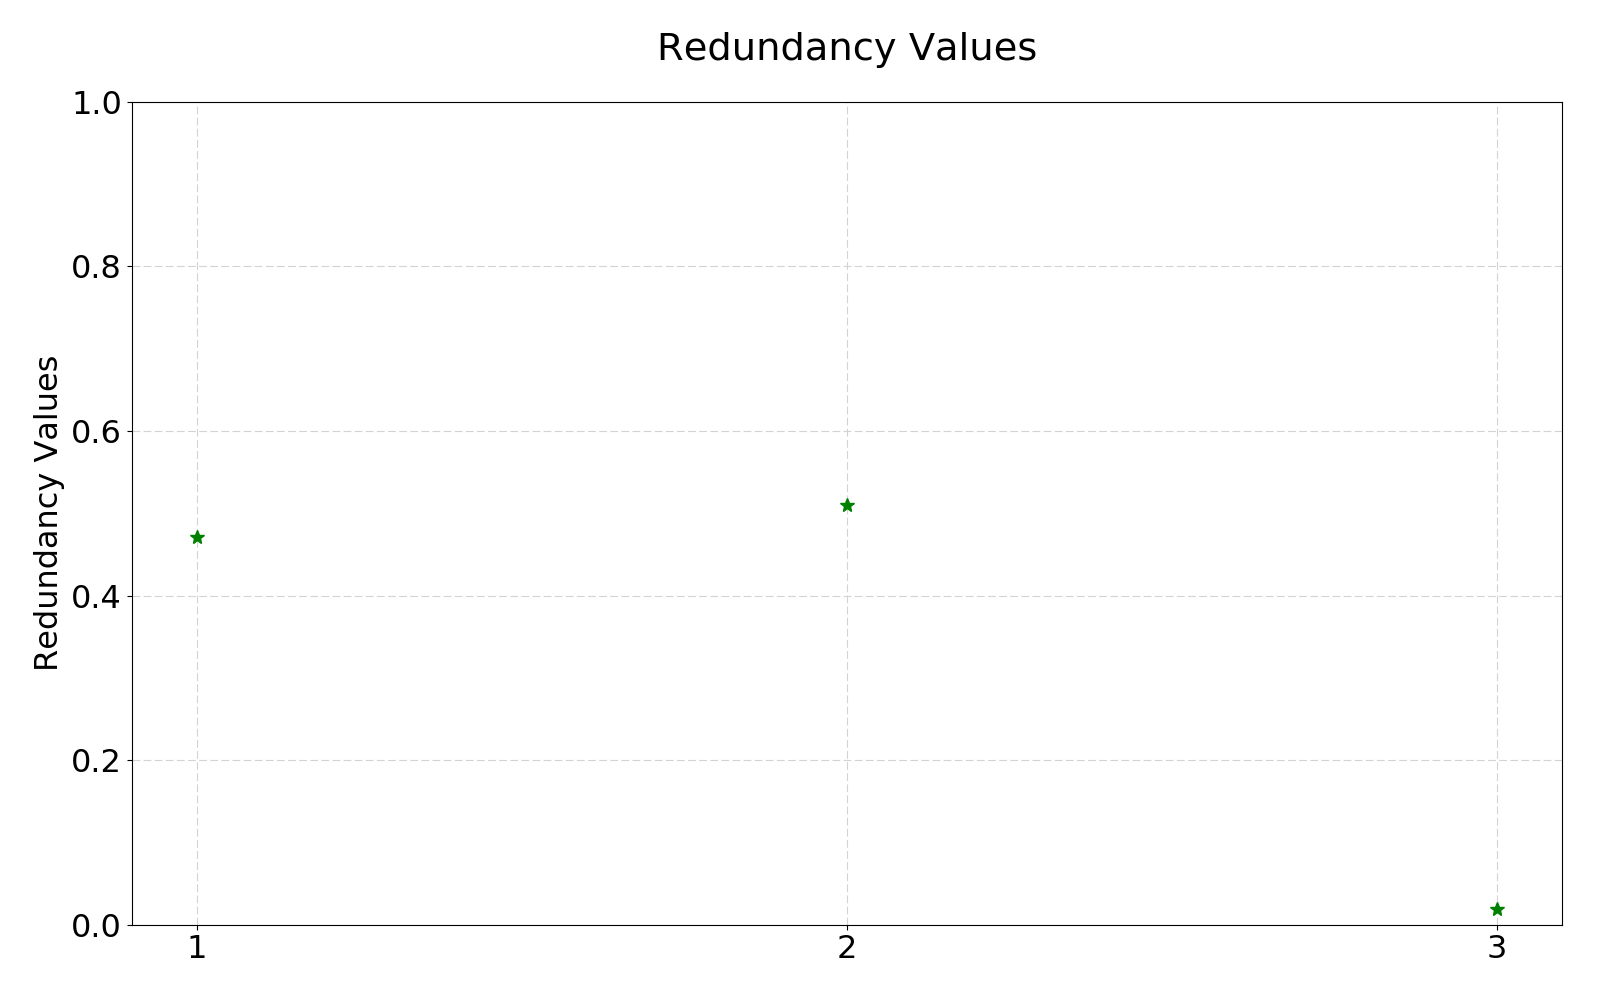
\includegraphics[trim = 0mm 0mm 0mm 0mm, clip, width=1.0\textwidth]{figures/ReliabilityExample/v22/Redundancy.png}
    \caption{Angles example - redundancy values}
    \label{Fig:Ex2redundancy}
\end{figure}

\newpage

The minimum detectable bias values (internal reliability) for the three observations, as shown in figure \ref{Fig:Ex2minDetBias}, reveals how the third observation has a significantly larger magnitude due to the poor redundancy of that observation:

\begin{figure}[!htb]
    \centering
    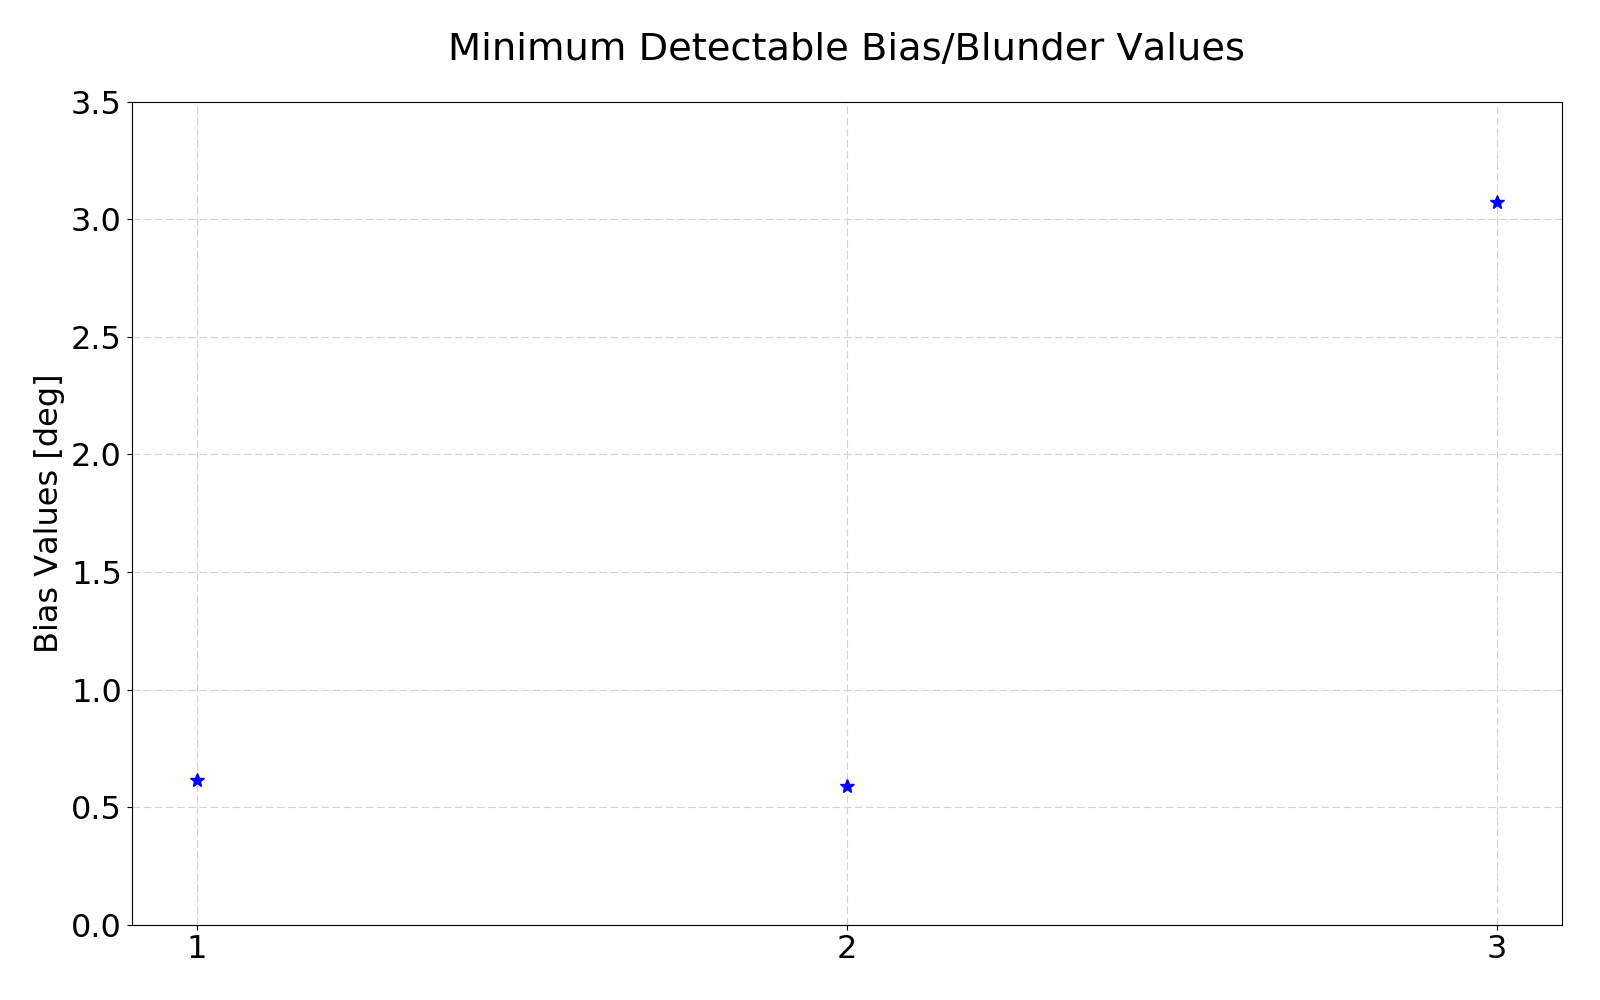
\includegraphics[trim = 0mm 0mm 0mm 0mm, clip, width=1.0\textwidth]{figures/ReliabilityExample/v22/MinDetBias.png}
    \caption{Angles example - minimum detectable bias values}
    \label{Fig:Ex2minDetBias}
\end{figure}

\newpage

The external reliability vector magnitudes for the three observations, as shown in figure \ref{Fig:Ex2ExtVectMag}, similarly shows the third observation has a much larger magnitude than the other two observations:

\begin{figure}[!htb]
    \centering
    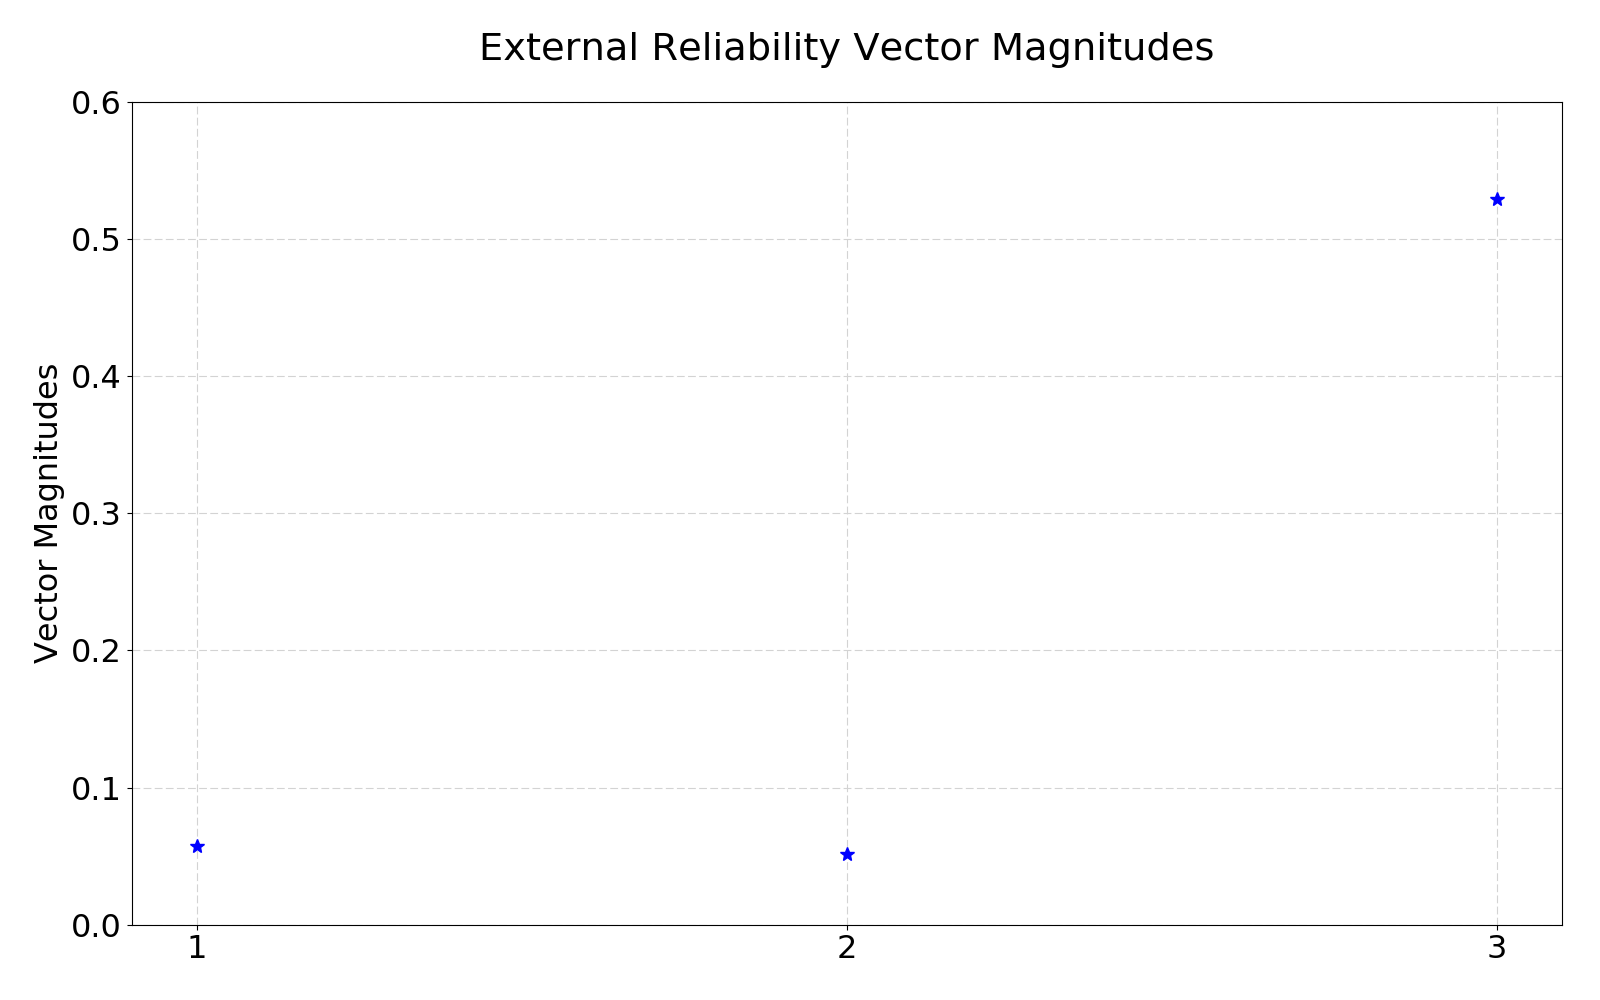
\includegraphics[trim = 0mm 0mm 0mm 0mm, clip, width=1.0\textwidth]{figures/ReliabilityExample/v22/ExtRelVectMags.png}
    \caption{Angles example - external reliability vector magnitudes}
    \label{Fig:Ex2ExtVectMag}
\end{figure}

\newpage

Just as in the ranges example above, the minimum detectable bias computed for the East station range observation is added to that observation, as shown in figure \ref{Fig:Ex2MapZoomBlunder}. The result: the estimated position now lies approximately on the northern edge of the reliability rectangle. (The estimated position lands exactly on the edge if no measurement noise is added.)

\begin{figure}[!htb]
    \centering
    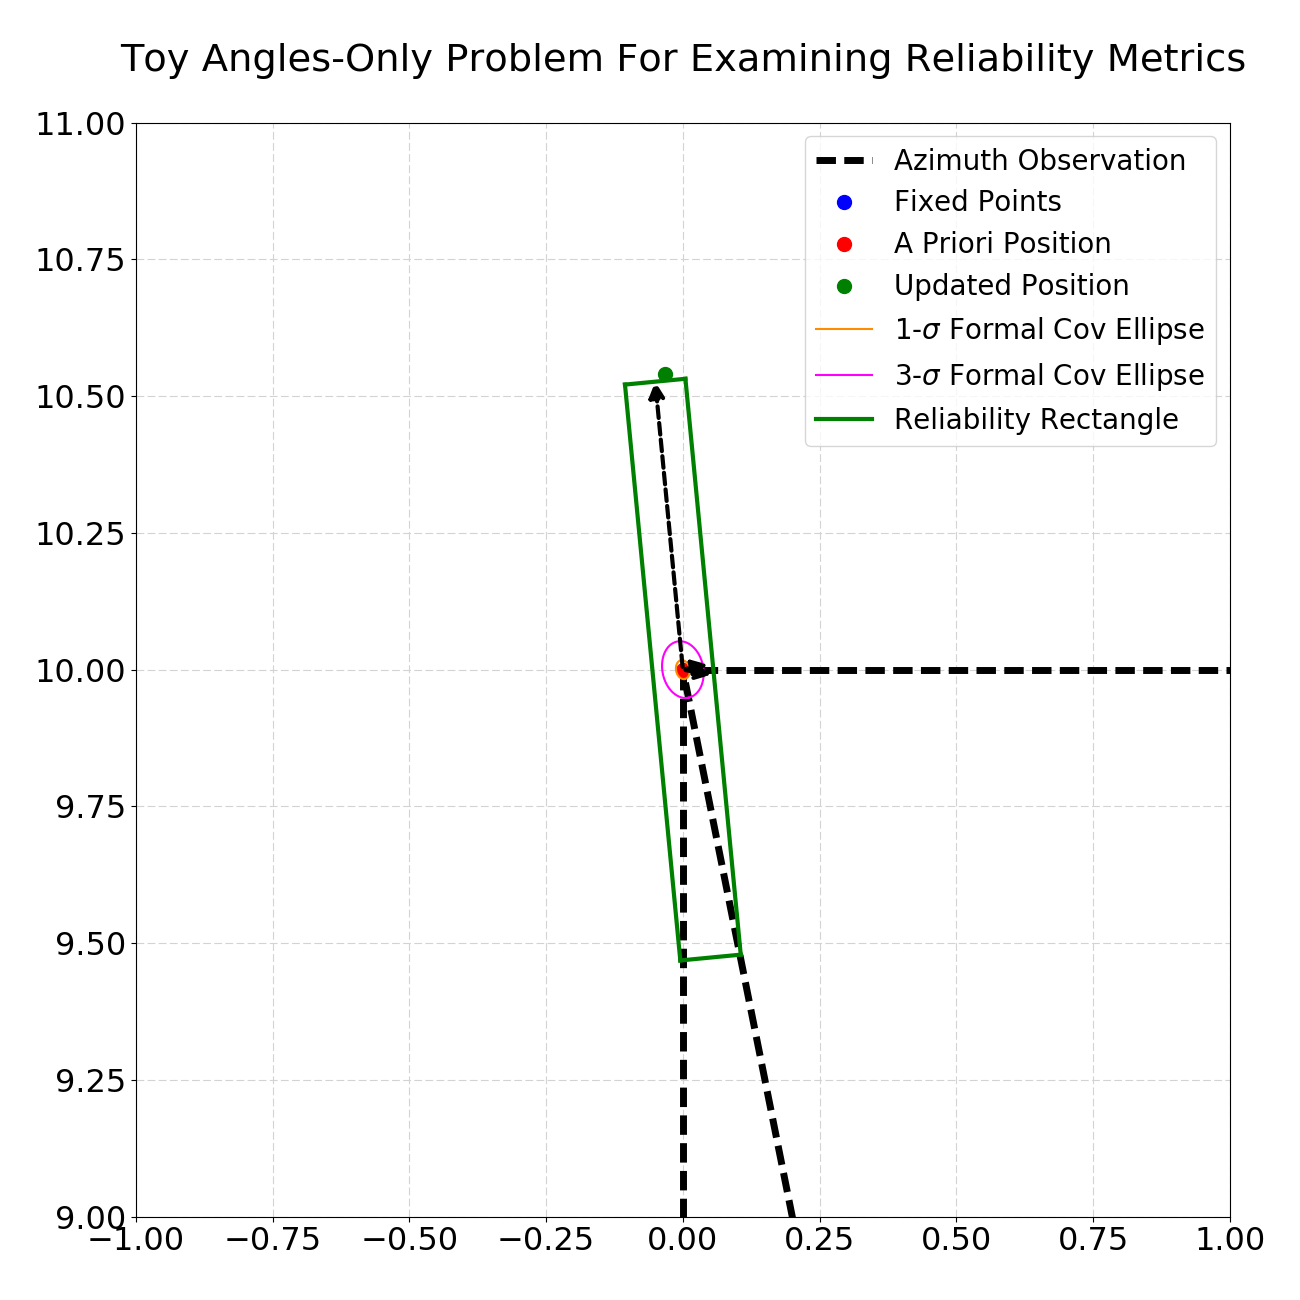
\includegraphics[trim = 0mm 0mm 0mm 5mm, clip, width=0.9\textwidth]{figures/ReliabilityExample/v26/MapZoomed.png}
    \caption{Angles example - east station blunder}
    \label{Fig:Ex2MapZoomBlunder}
\end{figure}

\newpage

Again just as in the ranges example above, the standard residuals do not reveal that the east station observation has a blunder, due to the lack of redundancy for that observation, as shown in figure \ref{Fig:Ex2StdRes}. 

\begin{figure}[!htb]
    \centering
    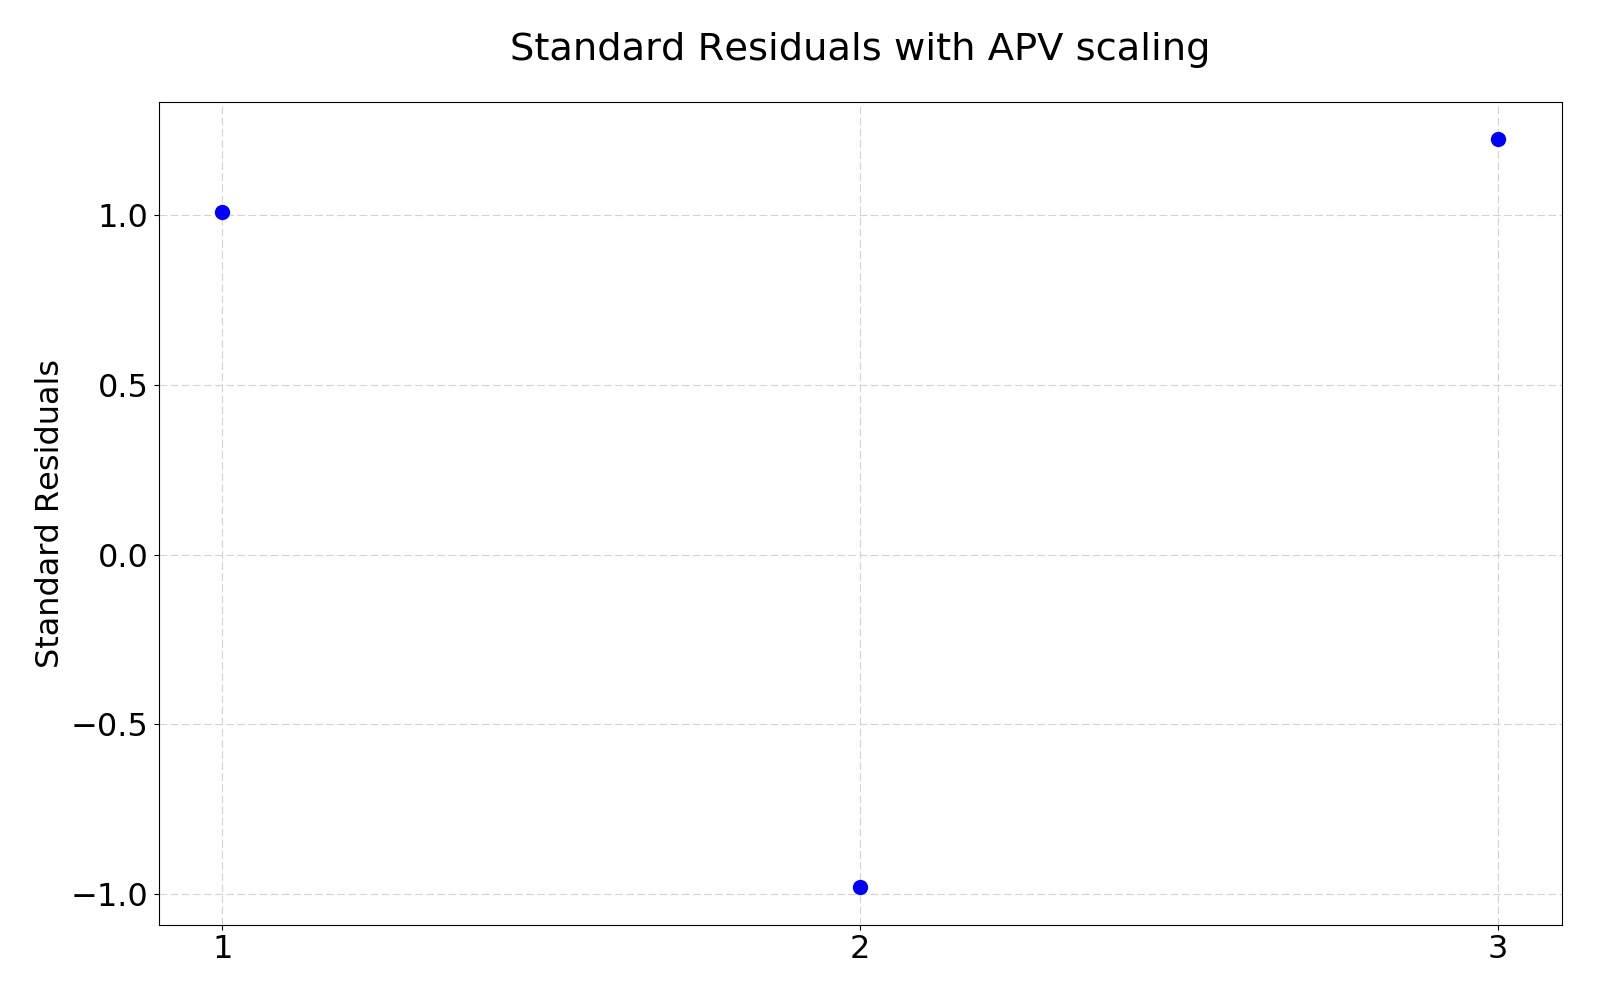
\includegraphics[trim = 0mm 0mm 0mm 0mm, clip, width=1.0\textwidth]{figures/ReliabilityExample/v56/StandardResidualsWithAPV.png}
    \caption{Angles example - standard residuals with east station blunder}
    \label{Fig:Ex2StdRes}
\end{figure}

\newpage

To address the lack of redundancy, another station can be added to the east, as shown in figure \ref{Fig:Ex2AddedObsMap}. 

\begin{figure}[!htb]
    \centering
    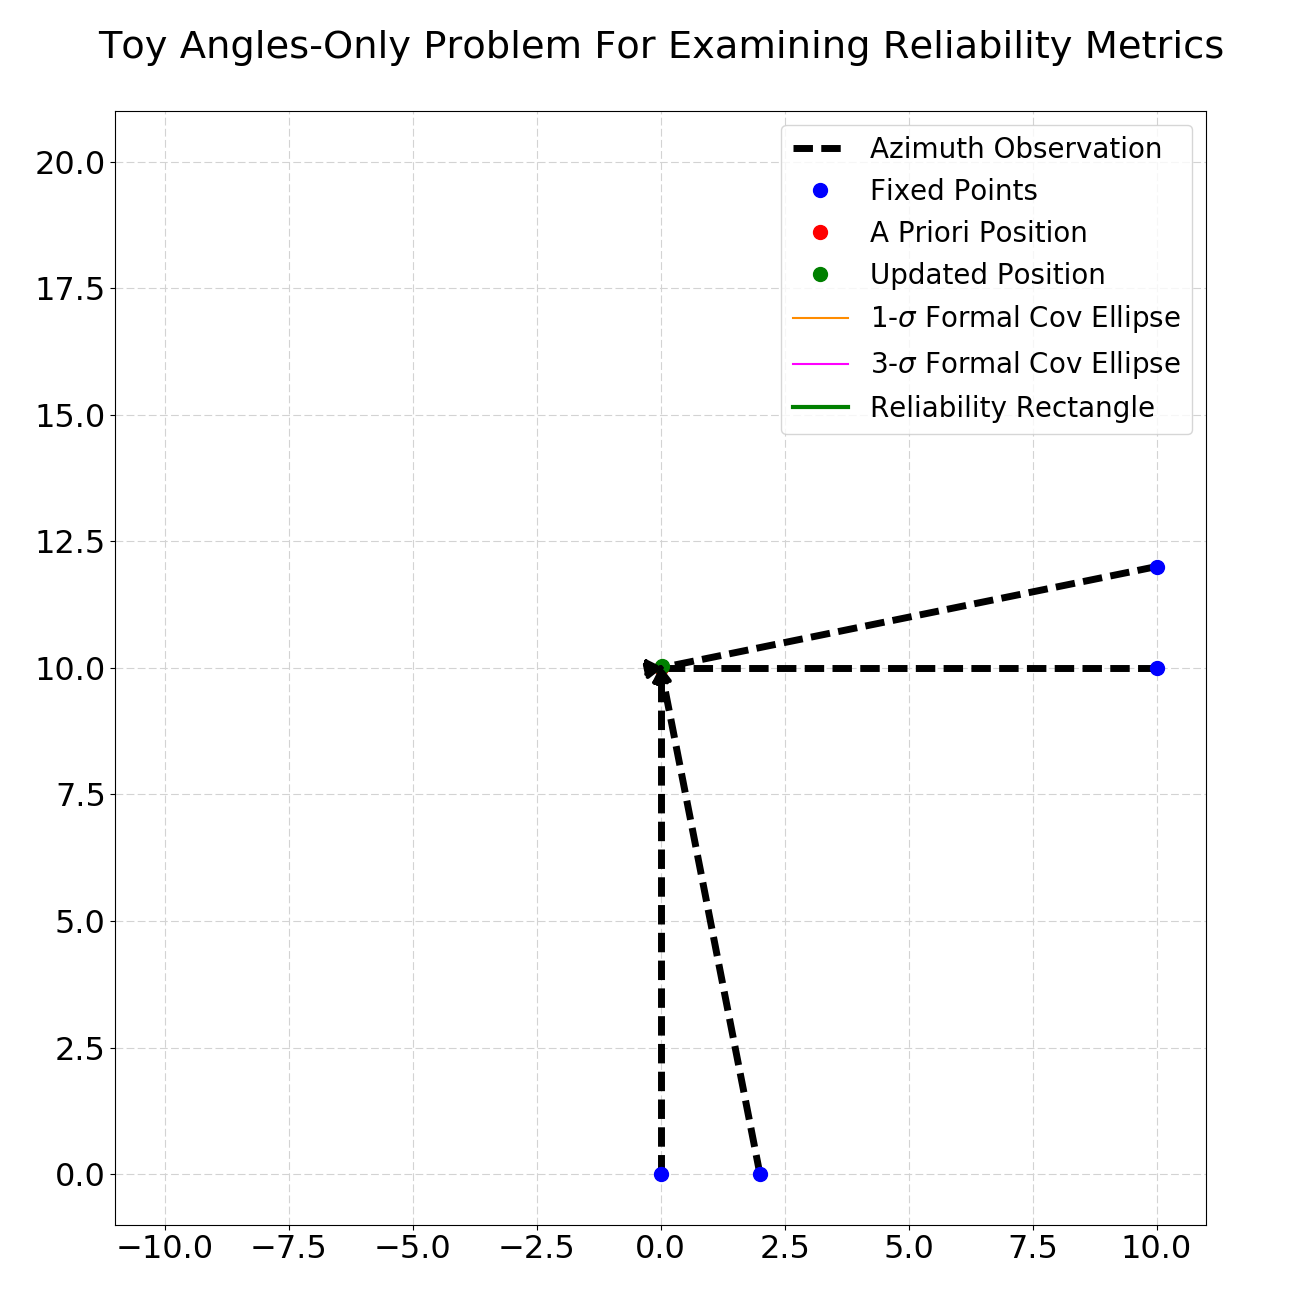
\includegraphics[trim = 0mm 0mm 0mm 5mm, clip, width=0.9\textwidth]{figures/ReliabilityExample/v24/Map.png}
    \caption{Angles example - adding additional observations}
    \label{Fig:Ex2AddedObsMap}
\end{figure}

\newpage

Zooming in on the estimated position reveals the impact of this additional observation on the reliability rectangle, as shown in figure \ref{Fig:Ex2AddedObsMapZoom}:

\begin{figure}[!htb]
    \centering
    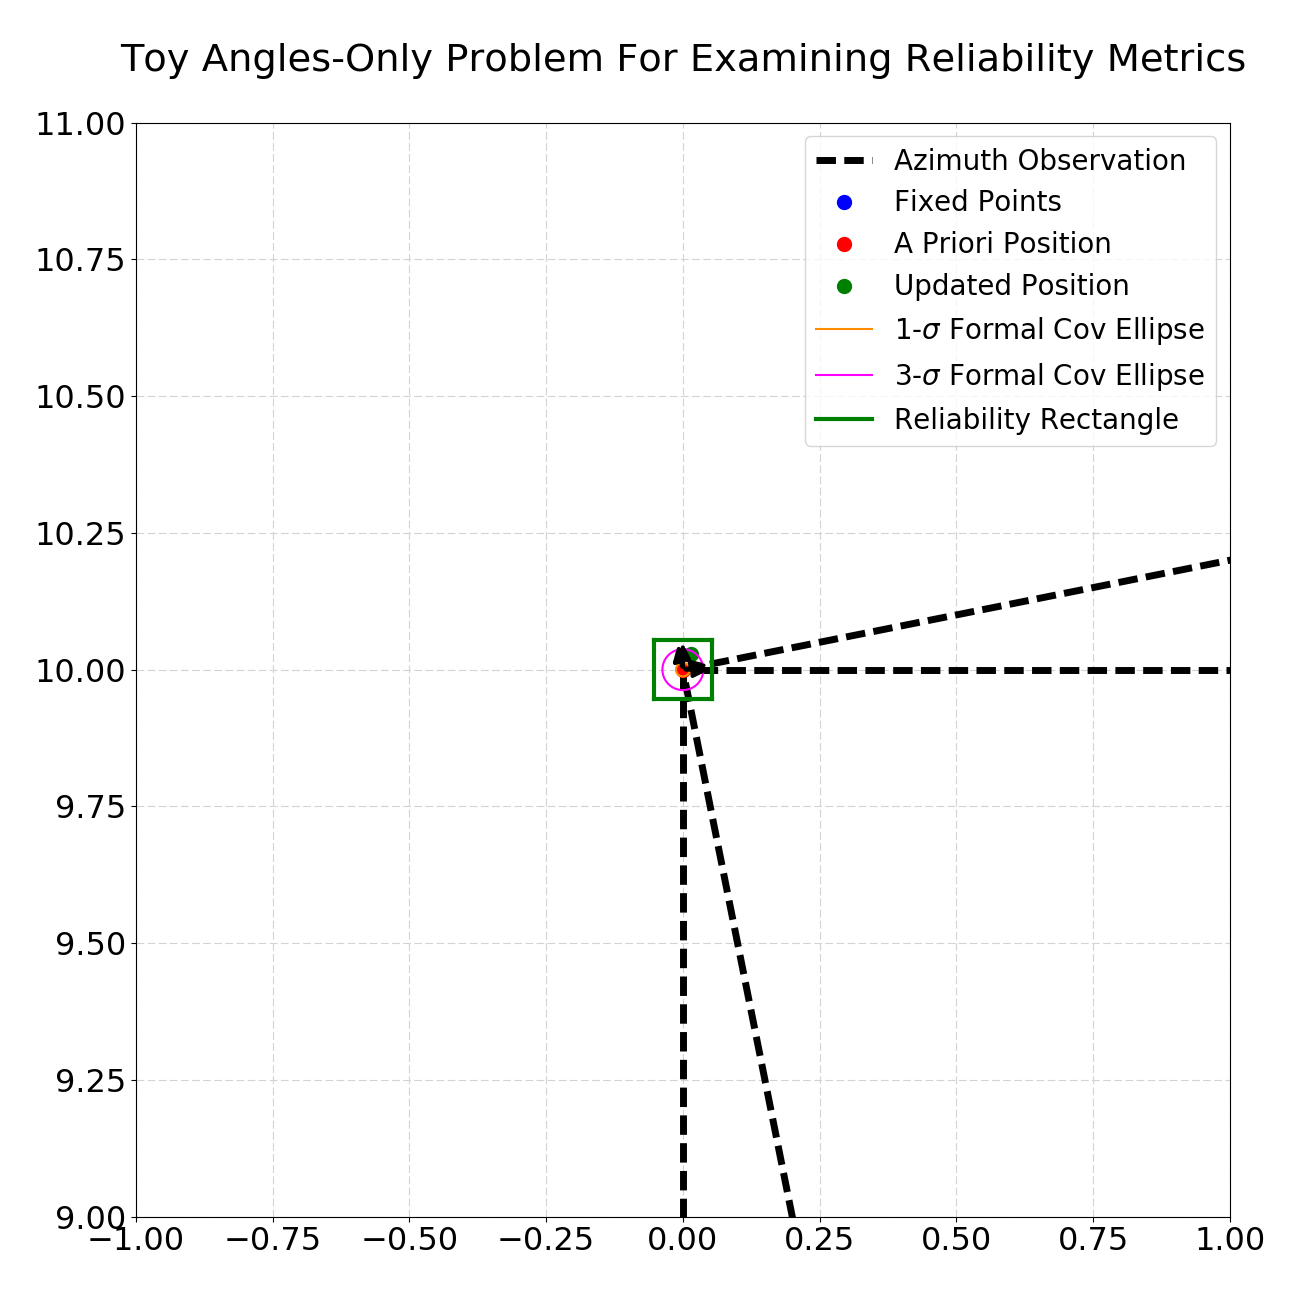
\includegraphics[trim = 0mm 0mm 0mm 5mm, clip, width=0.9\textwidth]{figures/ReliabilityExample/v24/MapZoomed.png}
    \caption{Angles example - adding additional observations}
    \label{Fig:Ex2AddedObsMapZoom}
\end{figure}

\newpage

\section{User Actions}

After an adjustment is processed, the surveyor should first verify that all observations have sufficient redundancy and no estimated points have unacceptably large reliability rectangles. Without good redundancy and reliability for each observation, metrics like standard residuals are not reliable indicators of potential blunders in the system.

Once good redundancy and reliability of all observations has been established, the standard residuals can be evaluated. If the standard residual test metric magnitude computed in equation \ref{eq:TestMetricStdRes} for a particular observation exceeds the threshold computed in equation \ref{eq:InvCDF}, the standard residual value is displayed as red text in the Measurement Residuals table. 

The user may wish to check each of these marked observations for blunders, with a focus on the data and/or sites involved in that measurement. Note that one blunder can affect many other quantities in the adjustment (estimated states and post-fit residuals). Thus the user is strongly encouraged to look for and correct only one blunder at a time, starting with the observation that has the largest standard residual test metric. After fixing that largest blunder, the user should re-run the adjustment and determine via the standard residuals (and other metrics such as the Chi-Squared Test) if more investigation is needed. Note that if the method of ``fixing'' the largest blunder results in poor redundancy/reliability, see above - the standard residuals may not be reliable anymore.

An important note: due to how the standard residual threshold is computed in equation \ref{eq:InvCDF}, if the redundancy value for an observation is low, the threshold value can become quite large. As a result, an observation with a large standard residual and low redundancy can still pass the hypothesis test and not be marked as red. Yet another reason it is vital to ensure all observations have reasonable redundancy. If the user encounters such an observation, we recommend the user collect more observations as needed to address the lack of redundancy in the survey itself if at all possible. If it is not possible, we recommend still investigating the largest residuals, even if they are not marked as failed the hypothesis test.

The user may also encounter smaller standard residuals that fail the hypothesis test and thus are marked as red. These observations likely have strong redundancy and small prescribed measurement uncertainty, and thus the relatively small raw residual is still large enough to fail the standard residuals hypothesis test. GPS vector observations often fall into this category, because GPS vector uncertainties are notoriously optimistic. Thus the user can likely ignore these relatively small standard residuals without significant impact on the final adjustment solution. If the user is feeling ambitious though, he or she can increase the prescribed uncertainty for that observation type, likely making that uncertainty more realistic and changing the standard residuals hypothesis test to passing.

One final note: the user should also keep an eye on the Chi-Squared global fit test to determine if there are any blunders remaining in the observations. If in the unlikely event there are large standard residuals but due to low redundancy values none of those residual fail the hypothesis test, it is like the Chi-Squared test will still fail.

% Maybe there is a smarter way to do this, i.e., one that would alphabetize itself... but here is a quick start.

\chapter{Definitions and Acronyms}

\begin{description}

\item[CG] Conjugate Gradient (least squares solution method)

\item[CLI] Command-Line Interface

\item[DMS] Degrees, Minutes, Seconds

\item[ECEF] Earth-centered Earth-fixed (Cartesian reference frame)

\item[GNSS] Global Navigation Satellite Systems

\item[GPS] Global Positioning System

\item[GUI] Graphical User Interface

\item[HDF] Hierarchical Data Format

\item[SALSA] Surveyor's Applications for Least Squares Adjustment

\item[SOA] Seconds of Arc

\item[SRIF] Square Root Information Filter (least squares solution method)

\item[WGS 84] World Geodetic System 1984

\end{description}

\chapter{Conversion of Instrumentation Output}
\label{chap:converters} % <-- I don't think this reference works since this is an appendix...

\section*{Instrument and File Types Supported}
At time of writing, \textsf{salsa} can import from the following instrument or file types; each of these converters is available under the Import menu:
\begin{itemize}
\item GeoLab format, typically \verb+.iob+
\item Leica Sets of Angles format, typically \verb+.log+ or \verb+.txt+
\item Trimble Data Exchange Format, typically \verb+.asc+
\item grape/merge Precise Point Positioning format, typically \verb+.log+
\item OPUS Precise Point Positioning format, typically \verb+.opus+
\item Leica Levels data, typically \verb+.gsi+. Both GSI-8 and GSI-16 data formats are supported.  Only BF and BFFB line leveling methods are currently supported.
\item Leica Geo Office ASCII exports, typically \verb+.asc+
\end{itemize}

\section*{Metadata}
When converting third-party instrument output files into \textsf{salsa}'s \verb+.lsa+ format, a comment will be placed at the top of the resulting \verb+.lsa+ file that indicates what converter was used to convert the file, what the source file was, and when the conversion took place.

Any information contained in the third-party output files that provides additional background on how that file was generated, such as the instrument type used, the instrument serial number, what version of software generated the output, when the file was generated, etc., will also pass through to the resulting \verb+.lsa+ file as a comment.

\section*{Order Preservation}
To the extent possible, records in the \verb+.lsa+ file will appear in the order that the information appears in the third-party instrument output file.  The order may not be exactly the same because some \verb+.lsa+ records require information that may be scattered throughout the instrument output file.  For instance, a ZANG record contains, in addition to the zenith angle measurement, the name of the From site, the instrument height offset at that site, the name of the To site, and the target height offset at that site.  This information may be scattered throughout the instrument output file, and it isn't until it has all been collected that the ZANG record can be written to the \verb+.lsa+ file.

\section*{Auto-generated Labels}
Some \verb+.lsa+ records are referred to by measurement records by their labels.  Examples of these records are instrument/target height offset records (HGHT), records describing the error model, including the centering errors, for a type of measurement (UNCR), and records that indicate of which set a particular set of directions are part (DGRP).  When created within \textsf{salsa}, using the Record Editor, the user may chose whatever descriptive label they wish for their referent records.  However, when converting from third-party instrument output files, these labels are auto-generated.  The scheme for generating these labels is as follows:

\begin{enumerate}
\item DGRP labels will appear in the \verb+.lsa+ as \emph{DGRP\#1}, \emph{DGRP\#2}, etc., in the order that sets of directions appear in the instrument output file.
\item HGHT labels will appear in the \verb+.lsa+ as \emph{HGHT\#1\_StationName},\\ \emph{HGHT\#1\_DifferentStationName}, \emph{HGHT\#2\_StationName}, etc.  The label will contain the station name, and the number will be incremented in the \verb+.lsa+ file depending upon how many times the instrument/target height offset at that station has been redefined.
\item UNCR labels will appear in the \verb+.lsa+ as \emph{UNCR\#1\_MeasurementType}, including the type of measurement in the label.  These labels are primiarily placeholders for the user to add additional information based upon their understanding of the instrument/target setup or measurement conditions.  As this information is not available during conversion, only one uncertainty record for a given measurement type will appear in each resulting \verb+.lsa+ file.  The default centering error for the At/From/To stations is set at 1 mm.
\end{enumerate}

\section*{Importing Into SALSA}
When inserting instrumentation output files into a \textsf{salsa} project via the Record $\to$ Insert $\to$ Include from... feature, \textsf{salsa} will automatically attempt to make the auto-generated labels unique to avoid duplication of labels throughout the project.  Therefore, if two instrument output files containing a single set of horizontal directions are inserted into a project, the first Include record in the project would contain an uncertainty record with a label of UNCR\#1\_HDIR, and a direction group label of DGRP\#1, while the second Include record in the project would contain an uncertainty record with a label of UNCR\#2\_HDIR, and a direction group label of DGRP\#2.

\section*{Leica Sets of Angles Measurement Uncertainties}
The user can configure the conversion process to assign default measurement uncertainties to the measurements in a \verb+.log+ or \verb+.txt+ file, or to accept the instrument-assigned uncertainties on the measurements (see Section \ref{subsect:convert_config}).  If the user opts to accept the instrument-assigned uncertainties, the following procedure is followed to derive the standard deviations of each measurement.  For a given \verb+Set Results+ section of the file (e.g. \verb+Horizontal Set Results+, \verb+Vertical Set Results+, and \verb+Distance Results+), containing some number of sets, \verb+N+, and some number of points:
\begin{enumerate}
\item The mean value of each measurement, $\overline{M}$, to a point is taken as the \verb+Mean of all Sets+ value for Vertical and Horizontal Sets, and the \verb+Mean Distance Of All Sets+ for Distances.
\item The individual measurements to each point, $M_{i}$, are taken as the \verb+Reduced Mean+ values for \verb+Hz Results Of Single Sets+, the \verb+Mean Of Face I/II+ values for \verb+V Results Of Single Sets+, and the \verb+Mean Of Face I and II+ values for \verb+Distance+ \verb+Results Of Single Sets+.
\item The standard deviation over N sets for measurement M to a point is then $\sigma=\sqrt{\frac{\sum_{i=1}^{N}\left(\overline{M}-M_{i}\right)^2}{N}}$.
\item If the calculated standard deviation for a direction happens to be less than 1 second of arc, then the standard deviation for that direction is set to the \verb+Standard Deviation Of Single Measurement+.  This covers the case when there is only one set, or when the reduced mean of a single set is 0 for all sets (which seems to be the case for the starting direction).
\item If the \verb+Mean Of Face I and II+ value for a distance measurement is zero, it is treated as the mean value when computing the standard deviation.
\end{enumerate}



\chapter{Understanding the Solver output}
\label{chap:solverout}

This Appendix describes, in more detail than the text in Chapter \ref{chap:UnderstandingSolver} ``Understanding the Solver,'' how to interpret parts of the output file of the solver. An example from a real, non-trivial run of the solver is presented and examined.

Consider the section of the solver output called ``Final Solution'' near the bottom of the file. This begins with a table of all the measurement data including measurements and residuals. The table is followed by a list of the three entries in the table with the largest standard residuals. Then comes the summary of statistics that is described in Chapter \ref{chap:UnderstandingSolver}.

[Note that the printed precision of numbers in this table is controlled by the solver options \verb+--linprec+ \verb+--angprecM+ and \verb+--angprecP+. In addition, the solver will also print this table at each iteration if the \verb+--verbose+ option is found (also with standard residuals if \verb+--statsAll+). See the solver command line reference Chapter \ref{chap:datref}.]

\newpage
\begin{landscape}
\fontsize{7.2}{7.2}
\begin{Snippet}
 Data and residuals (Final)
 Label                    Meas(m|DMS) Nomin(m|DMS) Pre-R(m|soa) Post-R(m|soa)   Rel-Res   Std-Res  Redund Int-Rel(m|SOA) Ext-Rel-E(m) Ext-Rel-N(m) Ext-Rel-U(m) Ext-Rel-Mag
 Del.T8(VNDP-OSS_TP1)X     -682.22620   -682.22080     -0.00181      -0.00540  -1.47760  -1.60865  0.5659        0.02058      0.01111      0.00349     -0.00251     0.01191
 Del.T8(VNDP-OSS_TP1)Y     1183.31220   1183.31748     -0.00145      -0.00528  -0.45181  -0.53724  0.4760        0.02615     -0.00888      0.00505     -0.00608     0.01189
 Del.T8(VNDP-OSS_TP1)Z     1215.35160   1215.35195     -0.00275      -0.00035  -0.73950  -0.90598  0.4427        0.01981      0.00122      0.00952      0.00449     0.01060
 Del.T9(5N-OSS_TP1)X      -3333.41390  -3333.42650      0.01619       0.01260   1.90033   1.66670  0.8686        0.03005      0.00313      0.00138     -0.00216     0.00404
 Del.T9(5N-OSS_TP1)Y      -3034.89880  -3034.91172      0.01675       0.01292   1.11493   0.95988  0.8963        0.03529     -0.00167      0.00195     -0.00258     0.00364
 Del.T9(5N-OSS_TP1)Z      -6138.44080  -6138.43635     -0.00685      -0.00445  -0.11113  -0.09554  0.9017        0.03134      0.00006      0.00269      0.00135     0.00301
 Del.T10(VNDP-OSS_TP2)X    -639.20240   -639.19906      0.17191      -0.00334  -0.83647  -0.88349  0.5973        0.02182     -0.00004      0.00472     -0.00173     0.01336
 Del.T10(VNDP-OSS_TP2)Y    1143.13750   1143.14303     -2.17457      -0.00553  -0.89714  -1.18186  0.3823        0.03075     -0.00190     -0.00173     -0.00529     0.01603
 Del.T10(VNDP-OSS_TP2)Z    1195.07860   1195.07789     -1.72257       0.00071  -0.22129  -0.29052  0.3888        0.02230     -0.00403      0.00244      0.00299     0.01318
 Del.T11(5N-OSS_TP2)X     -3290.38760  -3290.40476      0.19241       0.01716   2.39202   2.08804  0.8709        0.03236      0.00005      0.00148     -0.00159     0.00419
 Del.T11(5N-OSS_TP2)Y     -3075.06890  -3075.08617     -2.15177       0.01727   1.22928   1.05730  0.9039        0.03847     -0.00034     -0.00002     -0.00195     0.00375
 Del.T11(5N-OSS_TP2)Z     -6158.71370  -6158.71041     -1.72657      -0.00329   0.15504   0.13371  0.8955        0.03227     -0.00103      0.00047      0.00111     0.00329
 Del.T12(VNDP-OSS_TP3)X    -691.84980   -691.84291     -0.37619      -0.00689  -1.57596  -1.56023  0.6833        0.02238      0.00409     -0.00380     -0.00143     0.01174
 Del.T12(VNDP-OSS_TP3)Y    1158.97540   1158.98088     -2.77565      -0.00548   0.01523   0.01859  0.4480        0.03091     -0.00149      0.00792     -0.00441     0.01408
 Del.T12(VNDP-OSS_TP3)Z    1173.01550   1173.01021      0.04978       0.00529   0.88973   1.07754  0.4563        0.02135      0.00279      0.00257      0.00206     0.01116
 Del.T13(5N-OSS_TP3)X     -3343.03330  -3343.04861     -0.35399       0.01531   1.88901   1.61984  0.9083        0.03591      0.00121     -0.00072     -0.00123     0.00354
 Del.T13(5N-OSS_TP3)Y     -3059.23540  -3059.24832     -2.75725       0.01292   0.53935   0.45882  0.9245        0.04236     -0.00015      0.00161     -0.00165     0.00317
 Del.T13(5N-OSS_TP3)Z     -6180.78090  -6180.77809      0.04168      -0.00281   0.15331   0.13104  0.9171        0.03315      0.00061      0.00048      0.00100     0.00286
 Dis.T7(newPOSG-OSS_TP2)     26.00000     26.00413     -1.72816      -0.00413  -0.01376  -0.01124  0.9993        1.26625     -0.00002      0.00002     -0.00001     0.00007
 Han.T14(OSS_TP2-OSS_TP1)  62 41 38.0   62 41 39.5      -9866.8          -1.5      -0.2      -0.3  0.3036       55.19650      0.00262     -0.00296      0.00008     0.00395
 Han.T15(OSS_TP1-OSS_TP2) 311 46 17.9  311 46 20.7      -2440.1          -2.8      -0.4      -0.6  0.3112       51.56637     -0.00120     -0.00346      0.00002     0.00466
 Han.T16(OSS_TP1-OSS_TP3)  69  4 34.7   69  4 41.2       7421.3          -6.5      -0.5      -0.5  0.6983       66.00486     -0.00138     -0.00014     -0.00002     0.00195
 Zan.T17(OSS_TP1-OSS_TP2)  91  0  8.3   90 59 59.7      -1739.2           8.7       0.9       0.9  0.6543       51.56637     -0.00034     -0.00010      0.00243     0.00309
 Zan.T18(OSS_TP1-OSS_TP3)  93  9 35.9   93  9 35.6      -9234.2           0.4       0.0       0.1  0.3217       70.13019      0.00005     -0.00065      0.00403     0.00648
 Zan.T19(OSS_TP2-OSS_TP1)  89  0  8.7   89  0  2.4       1754.2           6.3       0.6       0.6  0.6543       51.56637      0.00034      0.00010     -0.00243     0.00309
 Zan.T20(OSS_TP2-OSS_TP3)  91 36 16.5   91 36 12.9      -5737.0           3.6       0.4       0.4  0.4995       59.81692      0.00047     -0.00024      0.00001     0.00490

 Largest 3 external reliability vector magnitudes:
 Del.T10(VNDP-OSS_TP2)Y    1143.13750   1143.14303     -2.17457      -0.00553  -0.89714  -1.18186  0.3823        0.03075     -0.00190     -0.00173     -0.00529     0.01603
 Del.T12(VNDP-OSS_TP3)Y    1158.97540   1158.98088     -2.77565      -0.00548   0.01523   0.01859  0.4480        0.03091     -0.00149      0.00792     -0.00441     0.01408
 Del.T10(VNDP-OSS_TP2)X    -639.20240   -639.19906      0.17191      -0.00334  -0.83647  -0.88349  0.5973        0.02182     -0.00004      0.00472     -0.00173     0.01336

 Largest 3 standard residuals (** denotes possible blunder: threshold based on Tau distribution and redundancy for each obs)
 Del.T11(5N-OSS_TP2)X     -3290.38760  -3290.40476      0.19241       0.01716   2.39202   2.08804  0.8709        0.03236      0.00005      0.00148     -0.00159     0.00419
 Del.T9(5N-OSS_TP1)X      -3333.41390  -3333.42650      0.01619       0.01260   1.90033   1.66670  0.8686        0.03005      0.00313      0.00138     -0.00216     0.00404
 Del.T13(5N-OSS_TP3)X     -3343.03330  -3343.04861     -0.35399       0.01531   1.88901   1.61984  0.9083        0.03591      0.00121     -0.00072     -0.00123     0.00354

 RMS post-fit relative residual (Final) = 9.37613e-01
 Degrees of freedom = 17; Std dev of unit weight = 1.22461; APV = 1.49967 (Final)
 RMS post-fit raw residual (angles) (Final) = 2.5e-05 rad = 5.1e+00 soa.
 RMS post-fit raw residual (length) (Final) = 9.11888e-03 m.
 Chi-squared test lower bound (0.050): 0.510 < 1.500 pass
 Chi-squared test upper bound (0.950): 1.500 < 1.623 pass
\end{Snippet}
\normalsize
\end{landscape}

\normalsize
Consider each of the columns of this table in turn (some of the column labels have been shortened in the table above to save space). 

\textbf{Column 1 Label.} This is the label that the solver uses to identify the measurements. It is of the form type.label(From-To)[XYZ], which consists of (a) the 3-letter measurement type from the input file (Dis = distance, Zan = zenith angle, etc.), (b) a unique label, which will be a number unless ``tag=label'' appears with the measurement in the input file, and (c) the labels for the Points involved in the measurement separated by dashes, usually just From-To, although horizontal angles will have From-At-To. Delta measurements (always in groups of 3) will also have a coordinate (X,Y,Z) at the end, since the measurement is a 3-vector.

For example, Del.T6(VNDP-TP1)Y is the Y-component of the delta measurement from Point VNDP to Point TP1; Zan.T16(TP1-TP3) is the zenith angle from Point TP1 to Point TP3.

\textbf{Column 2 Meas(m$\mid$DMS).} This is the measurement as read from the input file. Angles are expressed in DMS and linear measurements in meters.

\textbf{Column 3 Nomin(m$\mid$DMS).} This is the nominal or ``predicted'' value of the measurement, meaning the value computed using the current positions of all the Points.

\textbf{Column 4 Pre-R(m$\mid$soa).} The pre-residual is simply the difference ``Measured minus Nominal,'' using the current value for the Nominal (which is shown in column 3). In the final solution (after the last iteration) this means the Nominal as computed from the final adjusted Points. It is called ``pre'' because it is the data computed before (and passed into) the linear least squares algorithm.

\textbf{Column 5 Post-R(m$\mid$soa).} The post-residual is simply the difference ``Measured minus Nominal,'' using the \emph{a priori} value for the Nominal (not shown in the table); it is the total net residual after (hence ``post'') the adjustment. Thus if the \emph{a priori} position of a Point is not very good (e.g. it had to be computed by the solver), this post-residual may very well be large. 

\textbf{Column 6 Rel-Resid.} The relative residual is the output of the least squares solution algorithm at the latest iteration. Thus it indicates how much the measurement is ``in error'' according to the algorithm. This quantity is dimensionless, because the data given to the algorithm (and thus also its output) has been weighted (multiplied) by the inverse measurement covariance matrix. One can think of it roughly as the measurement residual in physical units divided by the given uncertainty in that measurement. (Of course this is a rough characterization because the division is actually a full matrix operation.)

\textbf{Column 7 Std-Resid.} The standard residual, actually a statistical test metric, is defined in appendix \ref{appendices:RedStdResComp}. This test metric is compared to a threshold computed using a 95\% confidence level. Standard residual values exceeding their respective thresholds are marked with ``**'' for the user, indicating a possible blunder within the survey adjustment network (so not necessarily within that measurement). The above table does not have any standard residuals exceeding their respective thresholds.

The three largest magnitude standard residual measurements are repeated in a subsequent table, prior to the statistical summary. Note that the standard residual is undefined for measurements with zero redundancy (which is very undesirable for any measurement in any survey), resulting in two dashes for the standard residual column value. 

\textbf{Column 8 Redund.} Redundancy is a number between 0 and 1 that is a measure of the immunity of the estimation to errors in the subject measurement. This column is the portion of the redundancy of the problem that belongs to this measurement; the sum of all the redundancies is equal to the degrees of freedom of the problem. Thus a large degree of freedom implies geometric strength in the estimation, and the geometry of the network and placement of the measurements are combined to ``divide up'' the total redundancy among the measurements.

It helps to think of redundancy in the two extreme cases. First, consider the case of zero redundancy. Suppose a DXYZ (GNSS vector) involves one fixed Point A and another unknown Point B; then if \emph{no} other measurements involve B, then the adjustment determines B simply by adding the DXYZ to A, and there is no more information pertaining to, and so no freedom to adjust, the measurement to Point B. The redundancy of the DXYZ will be zero (so will the pre-residual and relative residual, the standard residual is undefined).

Second, consider the case of high redundancy. Suppose one measurement involves two Points that also are involved in many other measurements. If you imagine perturbing that measurement, then the algorithm would respond by adjusting many other Points and measurements. The measurement is ``tied'' to many others through a strong network design. Conversely, all the other measurements to which it is tied will serve to improve the determination of the measurement's residual; redundancy in the network is necessary to identify the measurement as discrepant. Ghilani \cite{ghilani} has more discussion, including the derivation of redundancy.

\textbf{Column 9 Int-Rel.} Internal reliability, also known as the minimum detectable bias, is a quantity derived from redundancy. This is the minimum error value for a particular measurement which can be detected on the basis of elevated standard residuals.

\textbf{Column 10-12 Ext-Rel-*(m).} External reliability is calculated by mapping the internal reliability to state-space. Columns 10-12 represent the three components (East-North-Up) of the external reliability vector. 
 
\textbf{Column 13 Ext-Rel-Mag(m).} External reliability magnitude is the magnitude of the measurement's external reliability vector.  It is the Euclidean norm of the East, North, and Up components listed in the preceding columns.

%\section*{Record Types}
%The GeoLab user documentation\cite{geolab} lists the many record types supported by that application.  Many of those record types are not applicable in \textsf{salsa} or are otherwise not supported.  When a GeoLab \verb+.iob+ file is imported in \textsf{salsa}, the command-line application \textsf{iob2lsa} reads the \verb+.iob+ file(s) and generates corresponding \verb+.lsa+ files.  In doing so, the following record types are supported.  GeoLab record types not shown in this table are not supported in \textsf{iob2lsa}; warnings for unsupported record types will be shown in \textsf{salsa}'s status window.

\chapter{Inverse Configuration Parsing}
\label{chap:invConPar}

This chapter is meant to serve as an addendum to Chapter \ref{chap:StatInvDat} and provide the user with a more detailed explanation of how Salsa parses the \verb+*Inverses.cfg+ input configuration file. Some examples will also be provided to give the user some additional context into how the parsing works. The input configuration file is a plain text document which has one inverse station pair per file line. The station labels are delimited by space characters. Note that white space at the beginning and end of the lines are not important. If the user wishes to have spaces in the labels themselves they must encase the label string in double quotation marks ("). A table with some example input configuration lines and how they would appear in the Station Data Dialog box table can be seen below (note that \emph{blank} is used to reference an empty string)

\begin{table}[htb]
\caption{Sample Line Parse Results}
\label{tab:conParEx}
\begin{center}
\begin{tabular}{llp{2.5 in}}
\hline
\textbf{Sample Line} & \textbf{Table Output} & \textbf{Notes} \\
\hline
oneSite twoSite & [oneSite, twoSite] & \\
"one Site" "two Site" & [one Site, two Site] & Use of quotations preserves text \\
oneSite two Site & [oneSite, two] & Not enclosing two Site with parentheses leads to Site getting cut \\
oneSite twoSite threeSite ... & [oneSite, twoSite] & Everything after second space is ignored \\
oneSite \emph{blank} & [oneSite, \emph{blank}] & If string data is not provided on a line, empty string will be inserted \\
\emph{blank} \emph{blank} & [\emph{blank}, \emph{blank}] & \\
\hline
\end{tabular}
\end{center}
\end{table}

\chapter{Troubleshooting}

\section*{Bad Allocation}

\begin{figure}[!htbp]
\begin{center}
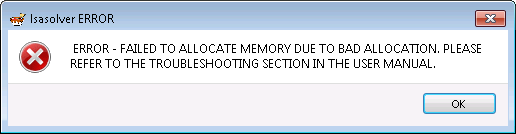
\includegraphics[width=0.5\textwidth]{badalloc_longmessage}
\end{center}
\caption{Error message for bad allocation.}
\label{fig:badalloc}
\end{figure}


A failure to allocate enough memory occurs in cases where \textsf{lsasolver} is unable to load the measurement data into RAM for processing.
This generally occurs when the project is large and the machine has limited physical RAM or if the machine has already allocated much of its available RAM for other tasks.
In some cases, it is possible to circumvent a memory limitation by increasing the amount of virtual memory available.
The amount of virtual memory needed will of course depend on the size of the least squares project.  In the developers' experience to date, projects with up to several thousand degrees of freedom usually run fine on typical desktop systems with a few GB of RAM, whereas projects with tens of thousands of degrees of freedom may require something on the order of 10 GB of additional virtual memory or more.  If 10 GB proves insufficient, additional virtual memory can be added so long as hard drive space permits.

\begin{figure}[!htbp]
\begin{center}
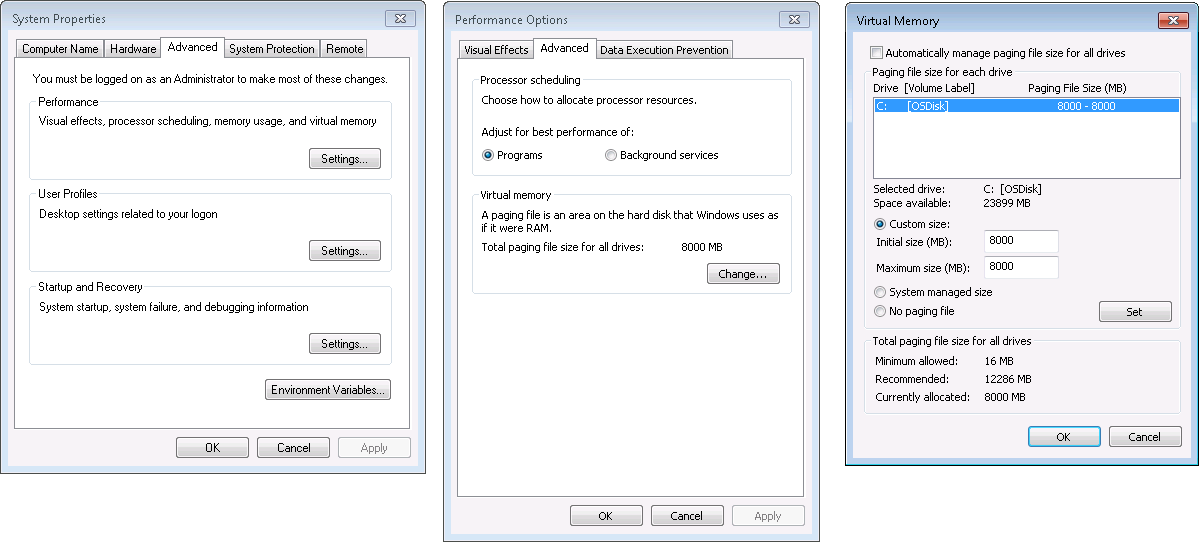
\includegraphics[width=1\textwidth]{vramsettings}
\end{center}
\caption{Dialog windows for setting virtual memory}
\label{fig:pagefilesettings}
\end{figure}

On Windows systems, the virtual memory is maintained in 
what is known as a \emph{paging file}.  A user with administrative privileges on a Windows 10 machine should be able to adjust the virtual memory by performing the following actions:

\begin{enumerate}
    \item Open Control Panel
    \item Go to \emph{System}
    \item Click on \emph{Advanced system settings} on the left pane
    \item Click on the \emph{Advanced} tab on the dialog
    \item Click on the \emph{Settings} button in the \emph{Performance} section
    \item Click on the \emph{Advanced} tab on the dialog
    \item Click on the \emph{Change} button
    \item Specify a custom size for the paging file
    \item Click on \emph{OK} in all dialogs to save settings and close
\end{enumerate}

\section*{Included file not found}

\begin{figure}[!htbp]
	\begin{center}
		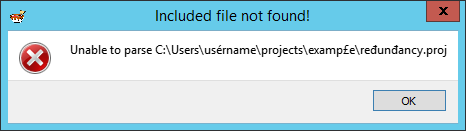
\includegraphics[width=0.6\textwidth]{unsupportedFilepath}
	\end{center}
	\caption{Error message from a bad filepath}
	\label{fig:badpath}
\end{figure}

A user may see a message (similar to figure H.3) indicating a failure to open/include a file due to one or more potential reasons. First, the file may not exist.  Open up a file explorer and navigate to the directory containing the file in question, to ensure it does indeed exist. Second, if that file does indeed exist, the failure may be due to the existence of special characters in the file path.  SALSA does not support special characters (e.g. £, é, ß) when opening files, and it is suggested that such files be renamed or moved to a directory containing ASCII only characters.

\section*{Solver Outputs and Points Files}

After calculating an adjustment for the first time, the user may have trouble viewing the .csv/.pts files via actions in the View menu. If the SALSA installation is on a Windows machine which has never had to open a .csv or .pts file, the OS may not have an executable associated with these file types. To resolve this, try to:
\begin{enumerate}
    \item Navigate to the project directory with the File Explorer
    \item Right click on the .pts/.csv file
    \item Select \emph{Open with...}
    \item A Windows menu (see \ref{fig:file_assoc}) should appear. Choose Notepad
\end{enumerate}

Following the above steps, any subsequent action to view the .pts file or Solver Output through the View menu should automatically open the file by launching Notepad. Notepad comes installed with the Windows OS and should be sufficient. Note that .csv files are more commonly opened with applications such as Microsoft Excel, which can be chosen instead of Notepad if installed on the user's machine.

\begin{figure}[!htbp]
\begin{center}
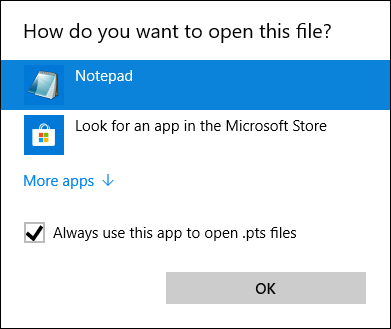
\includegraphics[width=0.5\textwidth]{file_assoc}
\end{center}
\caption{Windows file association dialog}
\label{fig:file_assoc}
\end{figure}

%\end{description}

\chapter{Third Party Software and Libraries}

\section*{Eigen}
The SALSA suite uses the Eigen math library \cite{eigenweb} version 3.4.0, licensed under the Mozilla Public License (MPL) version 2.0 \cite{MPL2}.  A copy of the MPL2 license is available alongside this User Manual, in the SALSA documentation folder.  The Eigen source code may be obtained from the Eigen web site, \url{http://eigen.tuxfamily.org/}.

\section*{GNSSTk}
The SALSA suite employs the GNSS Toolkit (GNSSTk) version 3.18 for geodetic transformations and many other functions.  The GNSSTk is licensed under the GNU Lesser General Public License version 3.0 \cite{LGPL}.  A copy of the GNSSTk license, including the LGPL and the GNU Public License that it references, is available alongside this User Manual, in the SALSA documentation folder.  The GNSSTk source code may be obtained from the project web site, \url{https://github.com/SGL-UT/GNSSTk}.

\section*{HDF5}
The SALSA suite makes use of the Hierarchical Data Format 5 (HDF5) software library \cite{hdf5}, developed by The HDF Group and by the National Center for Supercomputing Applications at the University of Illinois at Urbana-Champaign. The HDF5 copyright notice and license are available alongside this User Manual, in the SALSA documentation folder.

\section*{Marble}
The SALSA suite uses the Marble virtual globe and mapping library \cite{Marble} version 23.04, licensed under the GNU Lesser General Public License version 2.1 or later \cite{LGPL21}.  A copy of the Marble license is available alongside this User Manual, in the SALSA documentation folder. The Marble source code may be obtained from the Marble web site, \url{https://quickgit.kde.org/?p=marble.git}.

\section*{OpenSSL}
SALSA includes software developed by the OpenSSL Project for use in the OpenSSL Toolkit (http://www.openssl.org/).

\section*{Python}
SALSA is distributed with Python version 3.9 and numerous Python modules.  A copy of the Python Software Foundation License is available alongside this User Manual, in the SALSA documentation folder.  Individual modules' copyright and license texts are retained in or alongside the modules' source files.

\section*{QuaZIP}
The SALSA suite uses the QuaZIP library version 1.4 to interface with ZIP archives.  QuaZIP is licensed under the GNU Lesser General Public License version 2.1 \cite{LGPL21}.  A copy of the QuaZIP license is available alongside this User Manual, in the SALSA documentation folder. The QuaZIP source code may be obtained from the QuaZIP project page, \url{https://github.com/stachenov/quazip}.

\section*{Qt}
The SALSA suite uses the Qt application framework \cite{Qt} version 5.18.8, licensed under the GNU Lesser General Public License version 3.0 \cite{LGPL}.  A copy of the Qt license, including the LGPL and the GNU Public License that it references, is available alongside this User Manual, in the SALSA documentation folder. The Qt source code may be obtained from the Qt web site, \url{https://www.qt.io/}.

\section*{Qwt}
The SALSA suite leverages the Qwt project (\url{http://qwt.sf.net}) for 2D plotting features. Qwt is licensed under the GNU Lesser General Public License version 2.1 \cite{LGPL21} with exceptions to several of the conditions normally imposed by that license.  A copy of the Qwt license is available alongside this User Manual, in the SALSA documentation folder.

\end{appendices}

\end{document}
